%% LLT: Turn off some annoying warnings...
\RequirePackage{silence}
\WarningFilter{titlesec}{Non standard sectioning command}
\WarningFilter{scrreprt}{Usage of package}
\WarningFilter{scrreprt}{Activating an ugly workaround}

% **************************************************
% Document Class Definition
% **************************************************
\documentclass[%
	paper=A4,						% paper size
	twoside=true,					% onesite or twoside printing
	openright,						% doublepage cleaning ends up right side
	parskip=full,					% spacing value / method for paragraphs
	chapterprefix=true,				% prefix for chapter marks
	11pt,							% font size
	headings=normal,				% size of headings
	bibliography=totoc,				% include bib in toc
	listof=totoc,					% include listof entries in toc
	titlepage=on,					% own page for each title page
	captions=tableabove,			% display table captions above the float env
	draft=false,					% value for draft version
]{scrreprt}%

% **************************************************
% Debug LaTeX Information
% **************************************************
%\listfiles

% **************************************************
% Information and Commands for Reuse
% **************************************************
\newcommand{\thesisTitle}{Content and frequency of dream reports. Psychological and neurophysiological correlates.}
\newcommand{\thesisName}{Raphael Vallat}
\newcommand{\thesisSubject}{Neuroscience}
\newcommand{\thesisDate}{December 8, 2017}
\newcommand{\thesisVersion}{Draft}

\newcommand{\thesisUniversity}{\protect{Lyon 1 University}}
\newcommand{\thesisUniversityDepartment}{Department of Biology}
\newcommand{\thesisUniversityInstitute}{Lyon Neuroscience Research Center}
\newcommand{\thesisUniversityGroup}{Brain Dynamics and Cognition}
\newcommand{\thesisUniversityCity}{Lyon}
\newcommand{\thesisUniversityStreetAddress}{43 Boulevard du 11 Novembre 1918}
\newcommand{\thesisUniversityPostalCode}{69100 Villeurbanne}

\newcommand{\q}[1]{\textit{``#1''}} 	% Quote
\newcommand\fnurl[2]{\href{#2}{#1}\footnote{\url{#2}}} % Footnotes hyperlink

% **************************************************
% Load and Configure Packages
% **************************************************
\usepackage[utf8]{inputenc}
\usepackage{booktabs}
\usepackage{tabularx}
\usepackage{rotating}
\usepackage{ltxtable}
\usepackage{placeins}
\usepackage{multicol}
\usepackage[english]{babel} 	% babel system, adjust the language of the content
\usepackage{pdfpages}
\usepackage[					% clean thesis style
	figuresep=colon,
	sansserif=false,
	hangfigurecaption=true,
	hangsection=true,
	hangsubsection=true,
	colorize=reduced,
	colortheme=bluemagenta,
	% LLT: Use biber if using UTF8 encoding
	% bibsys=biber,
	bibsys=bibtex,
	bibfile=bib-refs,
	bibstyle=authoryear,
]{cleanthesis}

\hypersetup{							% setup the hyperref-package options
	pdftitle={\thesisTitle},			% 	- title (PDF meta)
	pdfsubject={\thesisSubject},		% 	- subject (PDF meta)
	pdfauthor={\thesisName},			% 	- author (PDF meta)
	plainpages=false,					% 	-
	colorlinks=false,					% 	- colorize links?
	pdfborder={0 0 0},					% 	-
	breaklinks=true,					% 	- allow line break inside links
	bookmarksnumbered=true,				%
	bookmarksopen=true					%
}

\urlstyle{same}

% Increase padding within table
\renewcommand{\arraystretch}{1.2}

% **************************************************
% Document CONTENT
% **************************************************
\begin{document}

% --------------------------
% rename document parts
% --------------------------
\renewcaptionname{english}{\figurename}{Fig.}

% --------------------------
% Front matter
% --------------------------
\pagenumbering{roman}						% roman page numbing (invisible for empty page style)
\pagestyle{empty}							% no header or footers

% \begin{titlepage}

  \setlength{\parindent}{0pt}
  \thispagestyle{empty}

  \begin{center}
  
\includegraphics[height=3cm]{content/logo}
  \end{center}

  \bigskip

  \begin{center}
  \fontsize{14pt}{16pt}\selectfont
  \textbf{THÈSE DE DOCTORAT DE L'UNIVERSITÉ DE LYON}\\

  \bigskip

  \fontsize{12pt}{14pt}\selectfont
  \textbf{Opérée au sein de}\\ \medskip
  l'Université Claude Bernard Lyon 1

  \textbf{École doctorale}\\ \medskip
  Neurosciences et Cognition (ED476)

  \textbf{Spécialité de doctorat}\\ \medskip
  Neurosciences

  Soutenue publiquement le 8 décembre 2017 par\\ \medskip
  \fontsize{14pt}{16pt}\selectfont
  \textbf{\thesisName}

  \rule{\textwidth}{0.5pt}

  \fontsize{16pt}{20pt}\selectfont
  \textbf{FRÉQUENCE ET CONTENU DU RAPPORT DE RÊVE:\\ \medskip
  Approches Comportementales et Neurophysiologiques.}
  \rule{\textwidth}{0.5pt}

  \end{center}

  \fontsize{12pt}{14pt}\selectfont
  \textbf{Devant le jury composé de:}

  \newcommand\textline[4][t]{%
      \par\noindent\parbox[#1]{.333\textwidth}{\raggedright#2}%
      \parbox[#1]{.333\textwidth}{\centering#3}%
      \parbox[#1]{.333\textwidth}{\raggedleft#4}\par
  }

  \textline[t]{Pr. Sophie SCHARTZ}{Université de Genève}{Rapporteure}
  \textline[t]{Pr. Michael SCHREDL}{CIMH}{Rapporteur}
  \textline[t]{Pr. Yves ROSSETTI}{Université de Lyon}{Examinateur}
  \textline[t]{Pr. Perrine RUBY }{Université de Lyon}{Directrice de thèse}

\end{titlepage}

\cleardoublepage
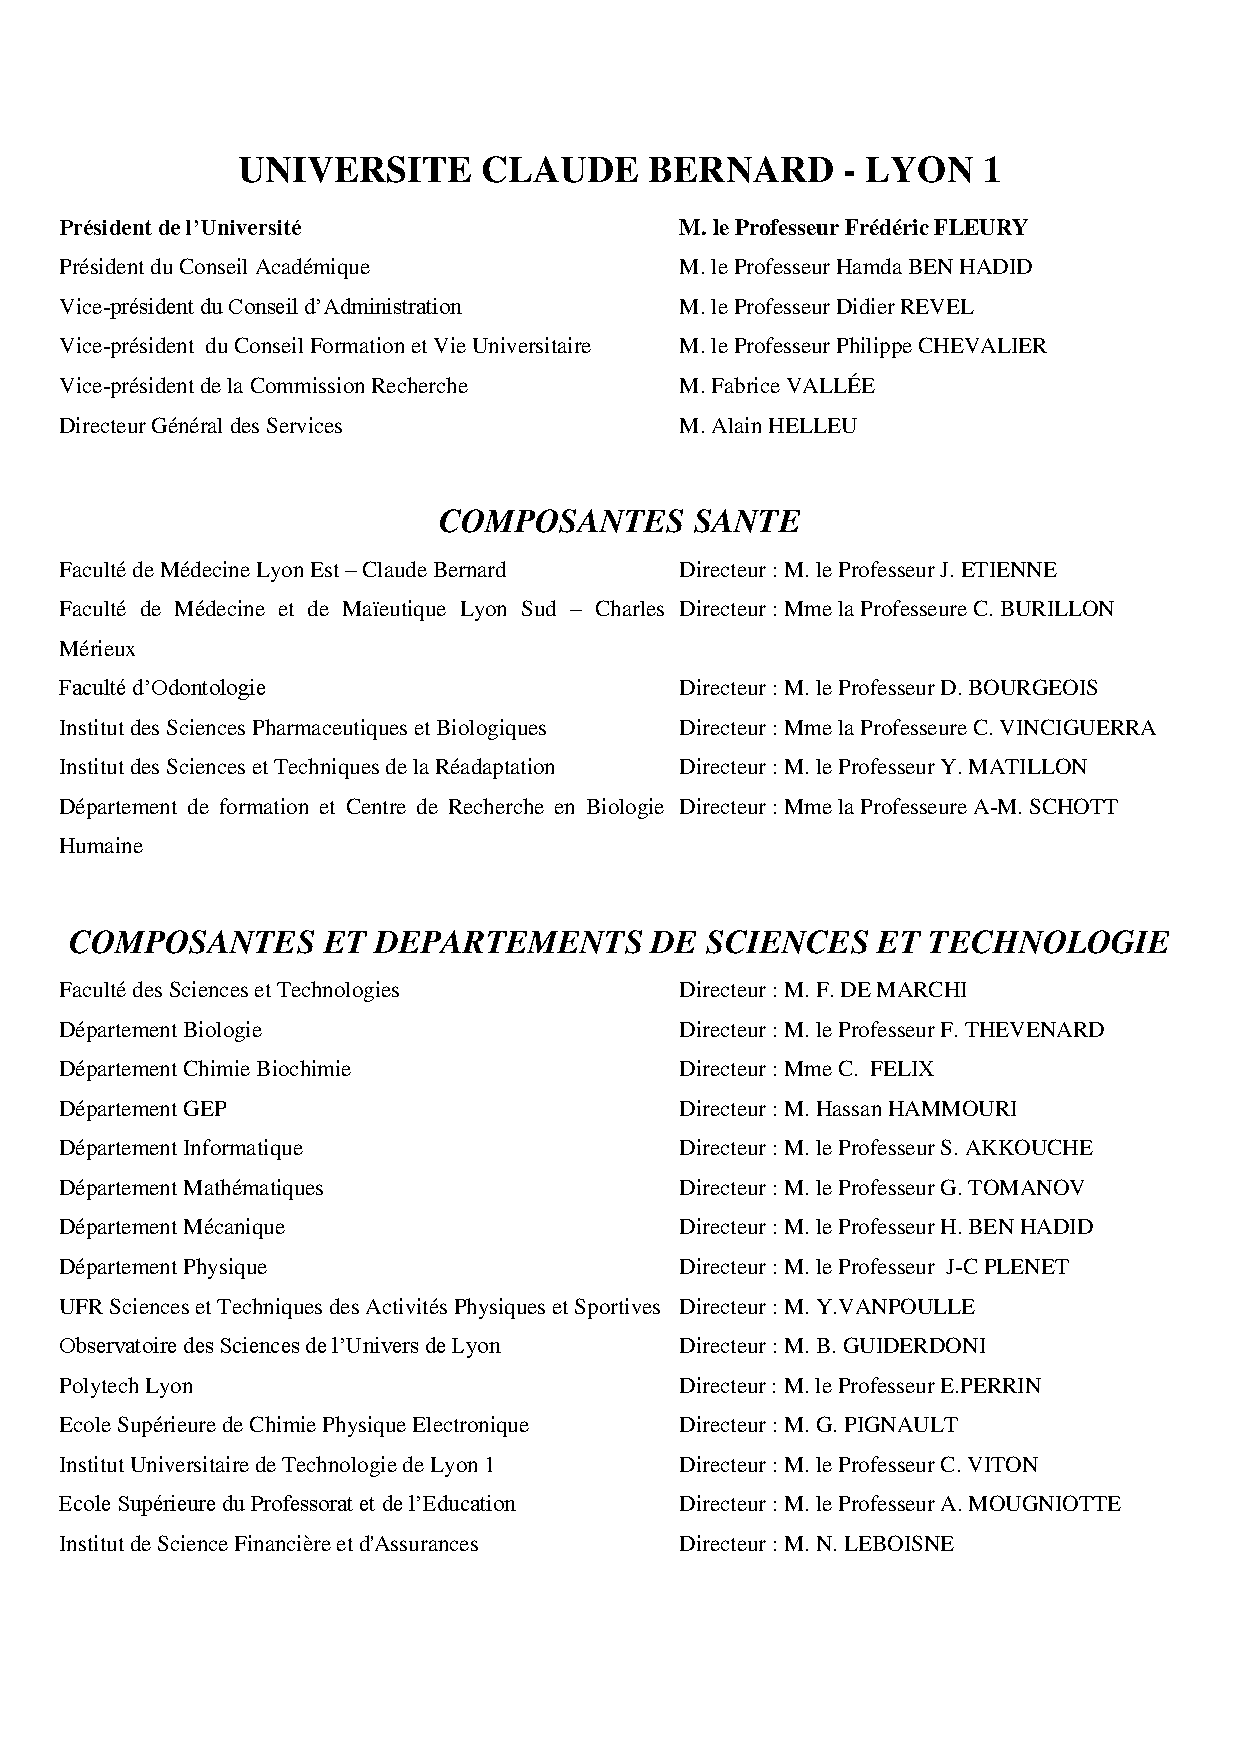
\includepdf[pages=-, fitpaper=true]{content/composante_lyon1.pdf}
			% Page de garde français + composante
% \cleardoublepage

% \begin{titlepage}

  \setlength{\parindent}{0pt}
  \thispagestyle{empty}

  \begin{center}
  
\includegraphics[height=3cm]{content/logo}
  \end{center}

  \bigskip

  \begin{center}
  \fontsize{14pt}{16pt}\selectfont
  \textbf{\uppercase{DOCTORAL THESIS OF LYON UNIVERSITY}} \\

  \bigskip

  \fontsize{12pt}{14pt}\selectfont
  \textbf{Delivered by}\\ \medskip
  \thesisUniversity

  \textbf{Doctoral School}\\ \medskip
  Neurosciences and Cognitive Sciences (ED476)

  \textbf{PhD specialty}\\ \medskip
  Neuroscience

  Publicly defended on the \thesisDate, by \\ \medskip
  \fontsize{14pt}{16pt}\selectfont
  \textbf{\thesisName}

  \rule{\textwidth}{0.5pt}

  \fontsize{16pt}{20pt}\selectfont
  CONTENT AND FREQUENCY OF DREAM REPORTS.\\ \medskip
  Psychological and Neurophysiological Correlates.
  \rule{\textwidth}{0.5pt}

  \end{center}

  \fontsize{12pt}{14pt}\selectfont
  \textbf{Jury:}

  Pr. Sophie Schwartz  	\hfill Reviewer\\
  Pr. Michael Schredl 	\hfill Reviewer\\
  Pr. Yves Rossetti 	\hfill Examiner\\
  Dr. Perrine Ruby 		\hfill PhD director\\

  \vfill

\end{titlepage}
			% Title page english
% \cleardoublepage
%
% \begin{figure}[htb]
    \captionsetup{labelformat=empty, skip=25pt, justification=raggedleft, boxcolor=white}
	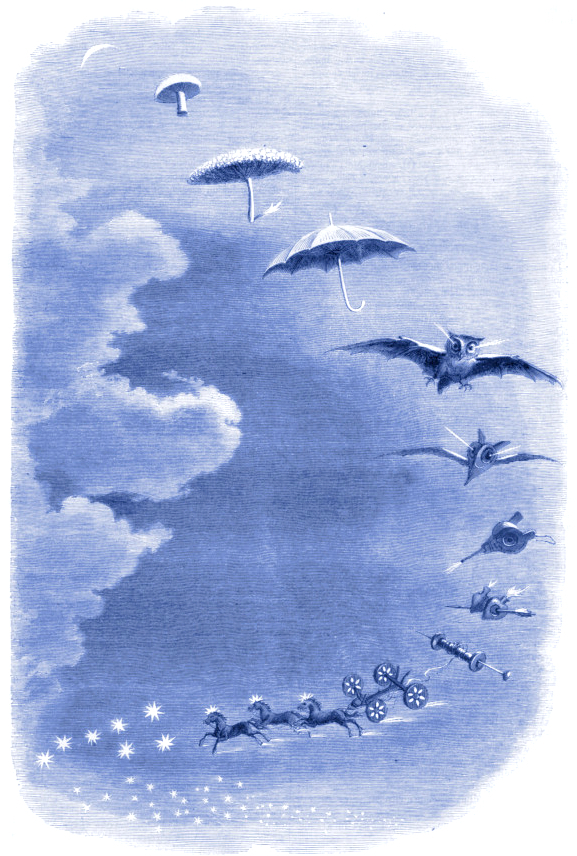
\includegraphics[width=\textwidth]{Artworks/Grandville_promenade.jpeg}
	\caption[]{
    --- \textbf{Jean-Jacques Grandville}\par
    Second rêve: une promenade dans le ciel. 1847
    }
\end{figure}

\cleardoublepage

%
% \pagestyle{plain}							% display just page numbers
%
% \addchap{Abstract}
\label{sec:abstract}
\vspace*{-10mm}

Since the dawn of time, humans have sought to understand the nature and meaning of their dreams. However, despite millennia of philosophical speculation and more than a century of scientific exploration, several questions regarding dreams remain pending.

One question that constitutes the core problematic of this thesis relates to why there are such individual differences in the frequency of dream recall, or in other words, why some people remember up to several dreams per morning (High-recallers, HR) while some hardly ever recall one (Low-recallers, LR). To characterize the cerebral and behavioral correlates of this variability, we compared the sleep microstructure (Study 1), as well as the brain functional connectivity in the minutes following awakening from sleep, a period marked by sleep inertia (Study 2). Among other results, we have shown that just after awakening, HR demonstrated a greater functional connectivity within regions involved in memory processes (default mode network). We proposed that this reflect a differential neurophysiological profile, which could facilitate in HR the retrieval of dream content upon awakening. Second, the numerous answers to the recruitment questionnaire of this study allowed us to conduct an epidemiological survey to characterize the sleep and dream habits of a large sample of French college students from Lyon 1 University (Study 3).

In another study, we focused on the relationships between waking-life and dream content (Study 4). Our results enhanced and refined our comprehension of the factors influencing the likelihood of incorporation of waking-life elements into dreams, and provided support for the hypothesis of an active role of dreaming in emotional regulation.

Lastly, we designed a free and open-source software dedicated to the visualization and analysis of polysomnographic recordings (Study 5), which aims at providing an intuitive and portable graphical interface to students and researchers working on sleep.

\textbf{Keywords}: Dream, sleep, awakening, memory, magnetic resonance imaging, electroencephalography, brain networks, software development

\cleardoublepage

\addchap{Résumé}
\label{sec:résumé}
\vspace*{-10mm}

Objet de nombreuses spéculations religieuses ou philosophiques, le rêve reste encore l'une des grandes terra incognita de la cognition humaine.

Une des questions récurrentes sur le rêve porte sur la grande variabilité de fréquence de rappel de rêve. En effet, alors que certaines personnes se souviennent de leurs rêves quotidiennement (« Rêveurs »), d’autres ne s’en souviennent que très rarement (« Non-rêveurs »). Le principal objectif de notre travail de thèse a été de caractériser les corrélats cérébraux et comportementaux de cette variabilité interindividuelle, en comparant entre ces deux groupes la structure du sommeil (Étude 1), mais aussi l’activité cérébrale pendant les minutes qui suivent le réveil (Étude 2). Nous avons entre autres montré que les « Rêveurs » faisaient preuve d’une plus grande connectivité fonctionnelle au sein du réseau par défaut et de régions impliquées dans des processus mnésiques dans les minutes suivant l’éveil, ce qui pourrait faciliter chez ces personnes le rappel et/ou la consolidation du rêve. Cette étude nous a également permis, grâce à l’analyse des nombreuses réponses obtenues au questionnaire de recrutement, de mesurer les habitudes de sommeil et de rêve chez un échantillon large d’étudiants de l’Université de Lyon 1 (Étude 3).

Dans une quatrième étude comportementale, nous nous sommes intéressés au lien existant entre la vie éveillée et le contenu du rêve. Nos résultats ont permis de mieux caractériser les facteurs influençant la probabilité d’incorporation des évènements de la vie éveillée dans le rêve, et ont mis en évidence l’importance du rêve dans des processus de régulation émotionnelle.

Finalement, en parallèle de ces travaux, nous nous sommes attachés au développement d’un logiciel gratuit de visualisation et d’analyse de tracés de polysomnographie, dont l’objectif est de fournir une interface intuitive et portable aux étudiants et chercheurs travaillant sur le sommeil.

\textbf{Mots-clés}: Rêve, sommeil, éveil, mémoire, imagerie par résonance magnétique, électroencéphalographie, réseaux cérébraux, développement logiciel
			% INCLUDE: the abstracts (english and french)
% \cleardoublepage
%
% \addchap{Acknowledgement}
\label{sec:acknowledgement}
\vspace*{-10mm}

Je tiens avant toute chose à remercier Perrine Ruby, ma directrice de thèse, dont la confiance et le soutien ont rendu possible ce travail. Tu sais, je l'espère, toute la considération et l'amitié que j'ai pour toi, et je ne te remercierai jamais assez de m'avoir toujours poussé vers l'avant, par exemple en me permettant de faire de nombreux congrès (et cela avant même de commencer ma thèse !). Ta rigueur et ton honnêteté scientifique, ainsi que ton engagement constant et indéfectible pour tes étudiants, sont tout autant de qualités que je souhaiterai avoir s'il m'est permis un jour d'encadrer des étudiants.

Ma pensée se tourne ensuite vers tous les membres du laboratoire DYCOG avec qui j’ai vécu et partagé des moments inoubliables tout au long de ces quatre dernières années. Sans pouvoir citer, par soucis écologique, toutes les personnes avec qui j’ai échangé, je tiens tout de même à évoquer mes collègues et amis du bureau d’en haut, Laurie-Anne, Kony, Etienne, Enrico, Stefano, dont la présence au Vinatier ne relève sans doute pas d’un hasard total ; les copains du café de 7 h et du saucisson de 19 h, Florian, Benoit, Thibault ; l’équipe des méditants Croix-roussien, Kristien, Antoine, Jelle, Oussama, pour ces moments de rire au milieu des fameux bouchons Lyonnais ; et bien sûr tous les autres doctorants, étudiants, ingénieurs, chercheurs, et personnels administratifs de ce laboratoire pour leur expertise scientifique et, surtout, leur bonne humeur qui rend la vie si agréable dans ce laboratoire.

Toute ma gratitude se porte également aux participants de nos expériences, d’imagerie ou de comportement, qui sont de fait la composante essentielle de ce travail. Ils nous ont prêté leurs rêves et leurs cerveaux, tout en gardant une motivation sans faille et un sourire constant.

Je pense ensuite à mes amis proches, Ylane, Caroline, Olivier, Géraud, Alex, Matthieu, Bertrand, qui ont su égayer ma vie durant toutes ces années, à coup de rires, de délires et de musique.

Le meilleur pour la fin dit-on - je remercie du fond du cœur mes parents, Isabelle et Alain ainsi que ma sœur Amélie et sa petite famille grandissante, sans qui tout cela n'aurait jamais été possible. Ma pensée finale se tournera vers Alisé, qui en plus d’être un sujet idéal pour étudier le sommeil au quotidien, est la personne avec qui je souhaite construire mes rêves.
 	% INCLUDE: acknowledgement
% \cleardoublepage
%
% \addchap{List of acronyms}
\label{sec:acronyms}
\vspace*{-10mm}

\begin{multicols}{2}

\textbf{DMN}: Default mode network

\textbf{DRF}: Dream recall frequency

\textbf{EEG}: Electroencephalography

\textbf{EMG}: Electromyography

\textbf{EOG}: Electrooculography

\textbf{fMRI}: Functional magnetic resonance imaging

\textbf{HR}: High-(dream)-recaller

\textbf{LR}: Low-(dream)-recaller

\textbf{MPFC}: Medial prefrontal cortex

\textbf{PET}: Positron emission tomography

\textbf{PSG}: Polysomnography

\textbf{TPJ}: Temporo-parietal junction


\end{multicols}

\textit{NB: These acronyms are always first defined in the text before being used as abbreviations.}
 			% INCLUDE: acronyms
% \cleardoublepage
%
% \addchap{Curriculum vitæ}
\label{sec:cv}
\vspace*{-10mm}

\textbf{Education and diploma}

2009: Scientific baccalaureate, \textit{cum laude}

2012: Bachelor degree of Cognitive Sciences, \textit{ranked 1st}, Lyon 2 University

2014: Master degree in Neurosciences, \textit{cum laude}, Lyon 1 University

2014–17: PhD program in Neurosciences, Lyon Neuroscience Research Center (CRNL)

2014–17: Teacher in Neurosciences (200h), Lyon 1 University

\textbf{Fellowship and awards}

2012: Two-year merit scholarship, from the French Ministry of Education

2014: Three-year PhD fellowship, from the French Ministry of Higher Education and Research

\textbf{Teaching activities}

Neurobiology \& Neuroanatomy, 1st and 2nd year of Bachelor Degree

Social science, 1st year of Medicine

Neuro-imaging, Master degree in Neuroscience

Supervision of two master students

Elected representative of the non-permanent members in CRNL council
 				% INCLUDE: short CV
% \cleardoublepage
%
% \addchap{List of publications}
\label{sec:publications}
\vspace*{-10mm}

\textbf{Peer-reviewed publications}

\underline{Vallat R.}, Lajnef T., Eichenlaub J.-B., Berthomier C., Jerbi K., Morlet D., and Ruby P. (2017). Increased Evoked Potentials to Arousing Auditory Stimuli during Sleep: Implication for the Understanding of Dream Recall. \href{https://doi.org/10.3389/fnhum.2017.00132}{Frontiers in Human Neuroscience}, 11.

\underline{Vallat R.*}, Combrisson E.*, Eichenlaub J-B., O'Reilly C., Lajnef T., Guillot A., Jerbi K. and Ruby P. (2017). Sleep: an open-source python software for visualization, analysis and staging of sleep data. \href{https://doi.org/10.3389/fninf.2017.00060}{Frontiers in Neuroinformatics}, 11. - \emph{* Co-first authors}

\underline{Vallat R.}, Chatard B., Blagrove M. and Ruby P. (2017) Characteristics of the memory sources of dreams: a new version
of the content-matching paradigm to take mundane and remote memories into account. \href{https://doi.org/10.1371/journal.pone.0185262}{Plos One}, 12. 

\textbf{Under review}

\underline{Vallat R.}, Meunier D., Nicolas A. and Ruby P. Reduced default mode network connectivity and anti-correlation in the minutes following awakening from N2 and N3 sleep: an EEG-fMRI study.

\underline{Vallat R.}, Eskinazi M., Nicolas A. and Ruby P. Sleep habits and dream recall frequency in a representative sample
of French students.

\textbf{In preparation}

\underline{Vallat R.}, Nicolas A. and Ruby P. Brain functional connectivity upon awakening from sleep predicts between-subject differences in dream recall frequency.

Combrisson E., \underline{Vallat R.}, O'Reilly C., Pascarella A., Saive A-L., Thiery T., Meunier D., Althukov D., Lajnef T., Ruby P., Guillot A. and Jerbi K. Visbrain: A multi-purpose GPU-accelerated open-source suite for brain data visualization.

Ruby P., Chatard B., \underline{Vallat R.}, Hoyer R. and Bidet-Caulet A. Top-down and bottom-up attentional processes in high and low dream recallers: an EEG study.

Plailly J., Villalba M., \underline{Vallat R.}, Nicolas A. and Ruby P. Recalling a dream related to a recent experience: does it help episodic memory consolidation?
 		% INCLUDE: publications
% \cleardoublepage
%
\makeatletter
\let\@cftmaketoctitle\relax
\let\@cftmakeloftitle\relax
\let\@cftmakelottitle\relax
\makeatother

% Table of contents
\setcounter{tocdepth}{1}		% define depth of toc
\addchap{Table of contents}
\vspace*{-10mm}
\tableofcontents
\cleardoublepage

% List of figures
\addchap{List of figures}
\vspace*{-10mm}
\listoffigures
\cleardoublepage

% List of tables
% \addchap{List of tables}
% \vspace*{-10mm}
% \listoftables
% \cleardoublepage

% --------------------------
% Body matter
% --------------------------
\pagenumbering{arabic}						% Arabic page numbering
\setcounter{page}{1}						% set page counter
\pagestyle{maincontentstyle} 				% fancy header and footer

% \part{GENERAL INTRODUCTION}
% !TEX root = ../thesis-example.tex
%
\chapter{Methods and problems in dream research}
\label{sec:dream-research}

\cleanchapterquote{Dream science holds an intermediate position between history and biology. It is a science of observation, because observation is an essential part of it, but it is also an historical science in the sense that the elapsed dream can never be reenacted and is therefore investigated, not directly, but through memory.}{Yves Delage}{Le rêve. Etude psychologique, philosophique et littéraire. 1920}

\section{Dreams}
\label{sec:dream-research:dreams}

\subsection{Definition}
\label{sec:dream-research:dreams:definition}

According to the Cambridge Dictionary, a dream is a \q{series of events or images that happen in the mind when one is sleeping}. This vague definition illustrates quite clearly how little we know about dreams, despite more than a century of experimental research and millennia of religious and philosophical speculation on their nature and meaning. The main reason for this lack of a clear and consensual definition (\cite{pagel_definitions_2001}) is that dreaming is \q{a phenomenon that we can solely observe during its absence} (Paul Valery, Analecta, 1926).  Indeed, we still do not know precisely when dreaming occurs during sleep, and the dreamer alone is witness to his or her dream. For that reason, the scientific study of dreaming relies critically on the introspective recall of the dreamer, or \q{retrospection} \citep{schwartz_dreaming:_2005}.

\subsection{Scientific perspective}
\label{sec:dream-research:dreams:science}

Therefore, a more scientific definition of dreaming was proposed by \citet{guenole_a_2009} who wrote that \q{dreaming is a mental experience during sleep, which can be remembered and reported at wake}. He further distinguished three successive and intertwined forms of the dreaming phenomenon. The primordial state is the dream-experience that happens during sleep, and of which very little is known because the dreamer has no means to communicate in real-time his or her oneiric experiences to the external world. With the notable exception of lucid dreaming, the dream-experience is unobservable to the waking consciousness, be it that of an external observer, but also that of the dreamer him- or herself. The second form is the memory of the dream-experience as we recall it after awakening. Importantly, the dream recall occur in a consciousness state different from the one in which the dream was experienced. As a memory object, dream recall is therefore likely to be influenced by several mechanisms such as forgetting, reconstruction, verbal description difficulties and censorships (\cite{schwartz_sleep_2002, schwartz_dreaming:_2005}). The third and last form is the dream report, obtained after transcription of the dream recall using words or pictures. The dream report is the only one that can actually be communicated to others and therefore the only one eligible to empirical investigation. As a consequence, most of the dream research has focused on dream reports.

\begin{figure}[htb]
	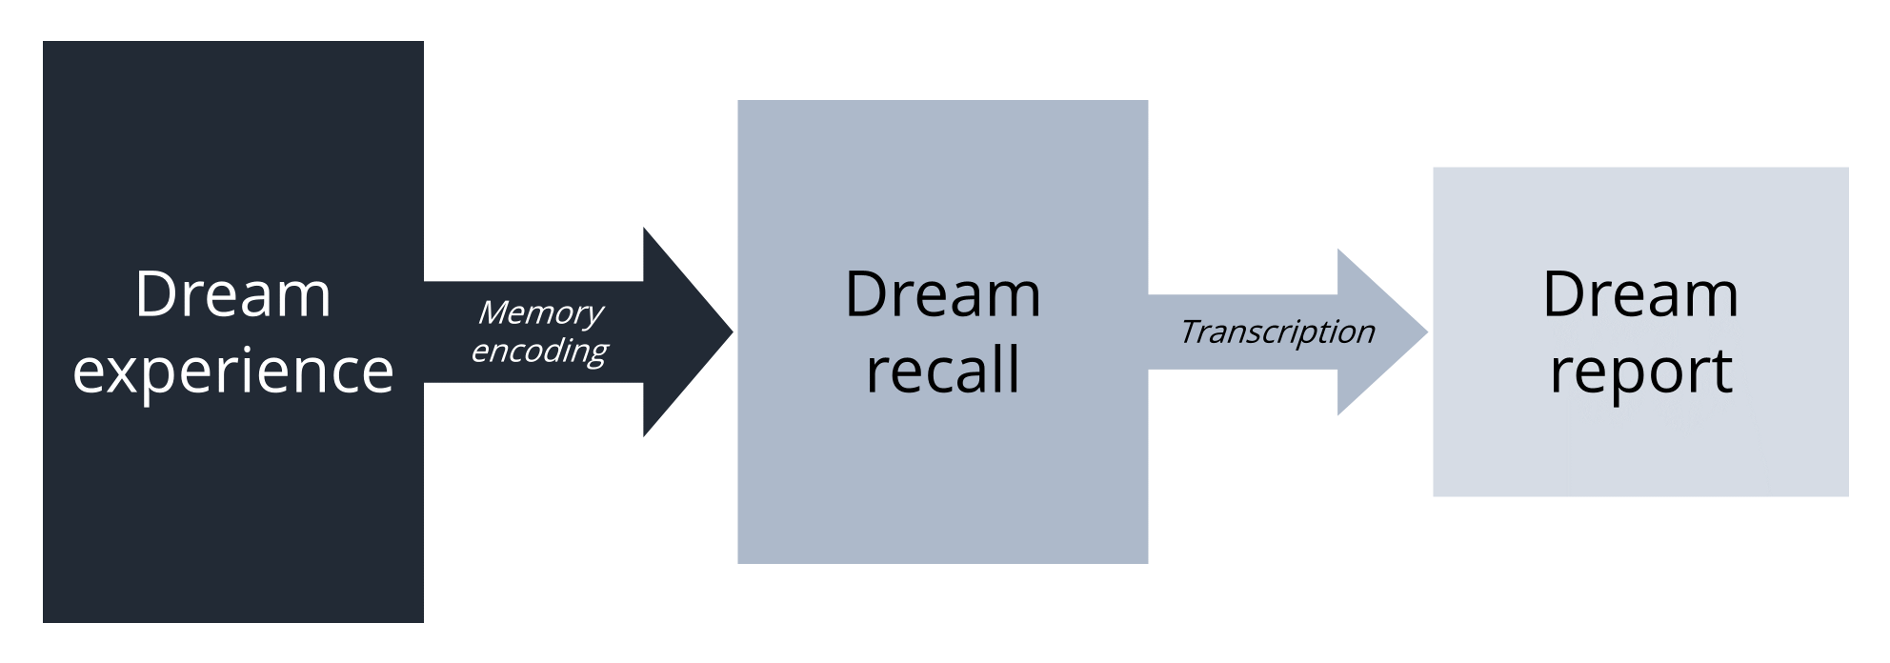
\includegraphics[width=\textwidth]{Fig/Intro/Intro_Guenole/Intro_Guenole.png}
	\caption[Guénolé's model of dreaming]{Guénolé's model of dreaming}
	\label{fig:intro:guenole}
\end{figure}

Because of this elusiveness of dreams and the constraints inherent to the scientific study of dreaming, it still remains one of the great mystery of the human cognition. Several questions on its nature and meaning are still not answered: do we dream every night? For how long? Why do we sometimes recall our dreams and sometimes not? Do dream reports obtained after awakening accurately convey subjective sleep experiences? What is, or what are, the function(s) of dreaming? What are the neurophysiological correlates of dreaming? The aim of the present thesis is to offer a modest contribution to the ongoing effort to solve these questions.

\section{Sleep}
\label{sec:dream-research:sleep}

As Schopenhauer rightly noticed, \q{the characteristic of dream is the condition of sleep peculiar to it}. Therefore, we cannot go any further in our study of dreaming without first defining the sleeping state and its physiology. Sleep is a normal physiological and periodic state characterized by vigilance suspension, which generally occurs during night time in humans. Sleep is a vital need that allows restoration of the immune, nervous, skeletal and muscular systems, leading some authors to postulate that \q{sleep is the price we pay for being alive} \citep{tononi_sleep_2014}. Long regarded as an idle state, it is becoming increasingly evident that sleep is \q{first and foremost a brain process} \citep{hirshkowitz_normal_2004} in which the brain is \q{hard at work and helps makes something of the world}, to borrow the words of Heraclitus’s famous aphorism (for an exhaustive review of the cognitive processes occurring during sleep, \citealt[see][]{andrillon_sleeping_2016}).

\subsection{Sleep stages}
\label{sec:dream-research:sleep:stages}

The invention of electro-encephalography (EEG) by Hans Berger in 1928 has paved the way for the scientific study of sleep. It was indeed soon after that discovery that Alfred Loomis first described a global slowing down of the brain rhythm during sleep, associated with the apparition of several grapho-elements such as K-complexes. Since then, sleep researchers have used EEG to monitor brain waves, electrooculography (EOG) to monitor eye movements and electromyography (EMG) to measure skeletal muscle activity. The simultaneous collection of these measurements is called polysomnography (PSG) and provides sufficient information to identify sleep stages according to standard international established guidelines. PSG is the gold standard in modern sleep science and is used in both clinical and research settings.

A first set of rules were published by Rechtschaffen and Kales (R\&K) in \citeyear{kales_manual_1968} and proposed to divide sleep into 5 stages with distinct electrophysiological properties, named rapid-eye movement (REM) and non-REM (NREM) stages 1, 2, 3, 4. This nomenclature was updated in 2007 by the American Academy of Sleep Medicine \citep{iber_aasm_2007} and sleep stage 3 and 4 have been merged into stage N3. Below are summarized EEG-EOG-EMG characteristics for wakefulness and the different sleep stages (see also Figure \ref{fig:intro:sleep_stage}).

\paragraph{Wakefulness}
Before diving into sleep, we first need to define the state of wakefulness. Eyes-closed quiet wakefulness is accompanied by an EEG rhythm predominantly in the alpha range (8-12 Hz). Opening the eyes or engaging in a significant mental task (for example mental calculation) reduces or blocks the alpha activity. Fairly high muscle activity can be present and slow or rapid eye movements may occur.

\paragraph{N1 sleep}
Stage N1 corresponds to the transitional period between wakefulness and sleep. The brain rhythm progressively decreases from alpha to theta (5 – 7 Hz), and the EOG is characterized by slow, rolling eye movements. N1 sleep represents approximatively 5\% of a normal night of sleep.

\paragraph{N2 sleep}
Each night, we spend more than half the night’s sleep in N2 sleep. The EEG activity during this stage is characterized by a predominance of theta waves, recurrently interrupted by two grapho-elements, the spindles and K-complexes, which are the landmarks of this sleep stage. K-complexes are defined as sharp negative waves followed by a positive component, prominent over frontal scalp electrodes and lasting more than 0.5 seconds. Spindles refer to burst of 12 to 14 Hz waves predominant over central scalp electrodes and lasting between 0.5 and 2 seconds. Beyond that, N2 sleep is characterized by an absence of eye movements as well as decreased muscle tone and brain metabolism.

\paragraph{N3 sleep}
N3 sleep, also referred to as deep sleep or slow-wave sleep, is the deepest sleep stage. It is characterized by a predominance (> 20\% of the epoch) of high amplitude (> 75 µV) delta waves (0.5 – 4 Hz). Eye motility, muscle tone and brain metabolism are even more decreased than in N2 sleep. N3 sleep represents approximatively 20\% of a normal night of sleep.

\paragraph{REM sleep}
As its name suggests, rapid eye movements (REM) sleep is characterized by rapid eye movements easily observable on the EOG channels. They consist of conjugate, irregular and sharply peaked eye movements, similar to some extent to those exhibited during wakefulness. Another fundamental aspect of REM sleep is its muscle atonia, as revealed by a low EMG activity. However, some transient muscle activity or muscle twitching (MTs) can also be observed. These short irregular bursts of EMG activity are superimposed on the background of low EMG activity. Brain metabolism is similar to that of wakefulness, and the EEG is marked by mixed low-amplitude waves predominantly in the theta band (saw-tooth waves), as well as a complete absence of delta rhythms. Other physiologic activities accompany REM sleep including middle ear muscle activity, periorbital integrated potentials, and sleep-related erections. REM sleep constitutes approximatively 20\% of a normal night of sleep.

\begin{figure}[htb]
	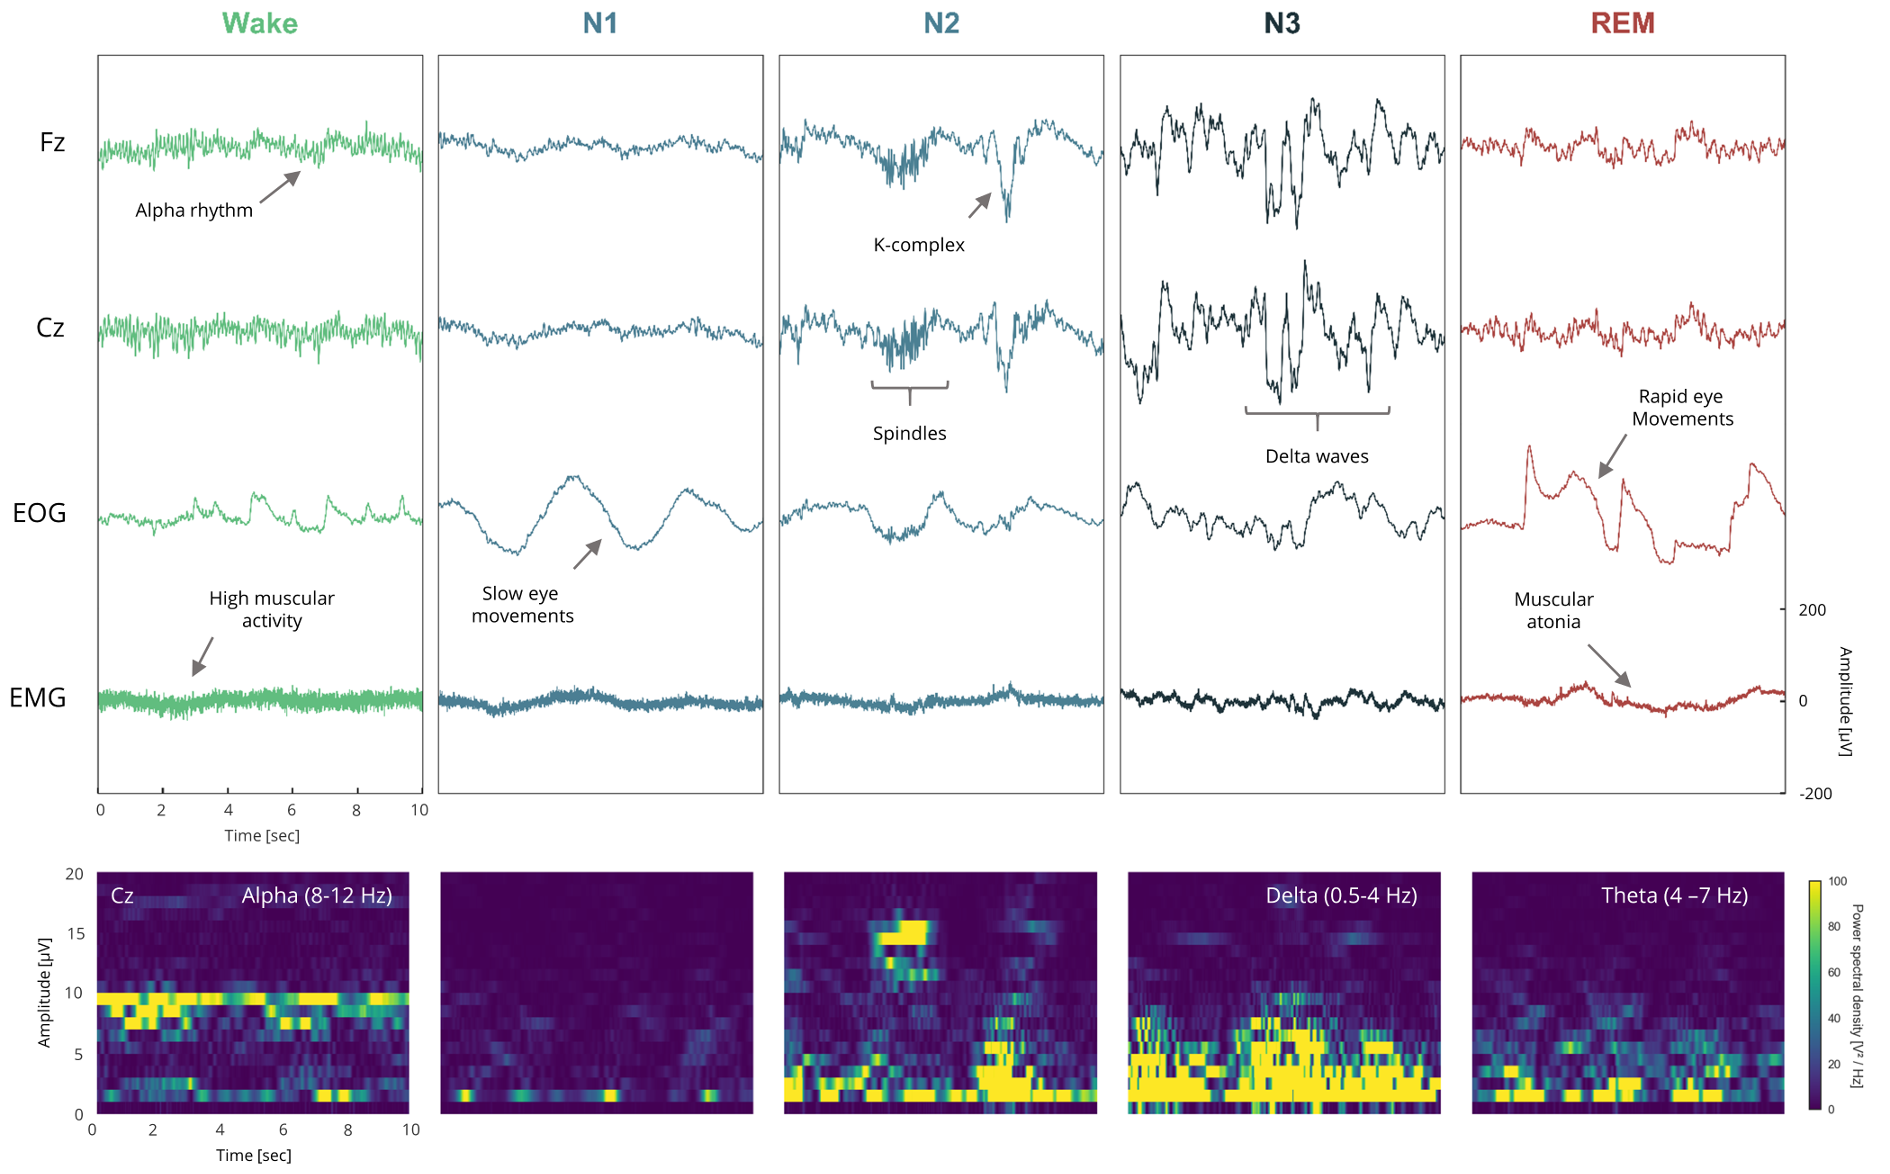
\includegraphics[width=\textwidth]{Fig/Intro/Intro_Sleep_Stages_PSD/Fig_Intro_Sleep_Stages_PSD_final_150517.png}
	\caption[Polysomnographic recordings across sleep and wakefulness]{Polysomnographic recordings across sleep and wakefulness. Top: Scalp EEG, EOG and EMG performed in one healthy young adult during wakefulness, N1, N2, N3 and REM sleep. The main features of each vigilance state are described. Bottom: Spectral properties of each stage obtained by computing the spectrogram of the Cz EEG signal atop.}
	\label{fig:intro:sleep_stage}
\end{figure}

\subsection{Sleep architecture}
\label{sec:dream-research:sleep:architecture}

Modern research has revealed that sleep is not a unitary, single block, but rather a cyclical succession of different brain states, which are all associated with specific functional roles. A normal night of sleep consists of a repetition of four or five 90 to 110 minutes long cycles in which sleep stages tend to follow each other in a particular order. The sleep cycle properties evolve with each cycle reoccurrence. Sleep staging is generally done visually by inspecting consecutive polysomnographic segments of 30 seconds. It results in a hypnogram which represents the succession of sleep stages across time (Figure 3). In his overview of the human sleep, Hirshkowitz described five generalizations about normal sleep architecture \citep{hirshkowitz_normal_2004}:

\begin{my_list_num}
    \item Sleep is entered through non-REM sleep
    \item Non-REM and REM sleep alternate approximately every 90 to 120 minutes
	\item N3 sleep predominates in the first third of the night
	\item REM sleep predominates in the last half of the night
	\item REM sleep occurs in four to six discrete episodes each night with episodes generally lengthening as sleep period progresses
\end{my_list_num}

\begin{figure}[htb]
	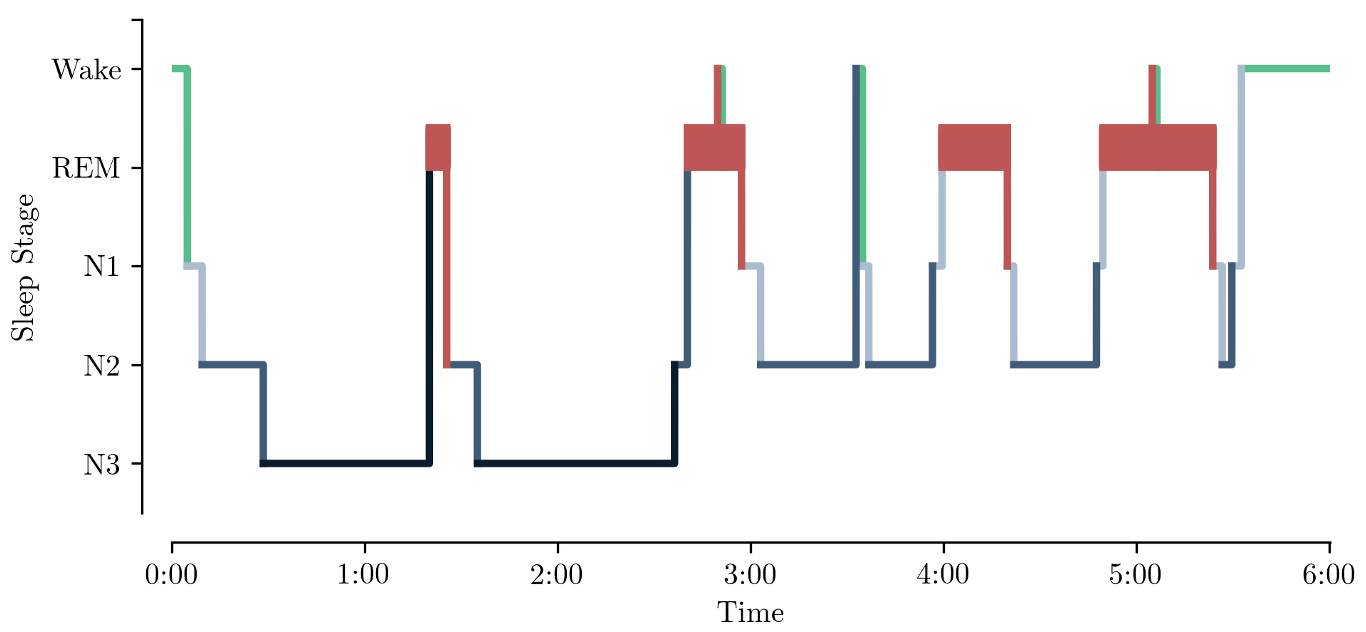
\includegraphics[width=\textwidth]{Fig/Intro/Intro_Hypnogram/Intro_Hypnogram.png}
	\caption[Example hypnogram of a healthy adult]{Example hypnogram of a healthy adult. The hypnogram is a graph which represents the stages of sleep as a function of time.One can easily recognize the succession of sleep cycles and especially the alternance of NREM (blue gradient) and REM sleep (red). Note that the hypnogram graph was generated directly as it is from the sleep software presented in the experimental results section.}
	\label{fig:intro:hypno}
\end{figure}

\section{Link between dreaming and sleep stages}
\label{sec:dream-research:link}

\subsection{The REM sleep hypothesis of dreaming}
\label{sec:dream-research:link:rem-sleep}

In the early fifties, Nathaniel Kleitman and his doctoral student Eugene Aserinsky, discovered in humans the existence of periods of sleep with an EEG similar to wakefulness (low voltage and fast frequencies), rapid eye movements and neurovegetative responses \citep{aserinsky_regularly_1953}. This discovery had a strong and persistent impact on dream and sleep research. The authors have indeed proposed that the rapid eye movements corresponded to the scanning of dream images. They reached this conclusion by comparing the proportion of dream reports obtained upon awakening in periods of eye motility and outside these periods, respectively 75\% and 11\% in their 1953’s study, and 80\% and 7\% in their 1957's study \citep{dement_relation_1957}. They concluded that their newly-discovered REM sleep stage was the neurophysiological basis of dreaming. A few years later, the French neurophysiologist Michel Jouvet, who had started working on sleep in cats, found that REM sleep was associated with muscular atonia \citep{jouvet_sur_1959}, a finding that was soon after replicated in humans \citep{berger_tonus_1961}. Pursuing his research on REM sleep, or \q{paradoxical sleep} as he named it, Jouvet had the idea to suppress the muscular atonia by injuring the brain stem of cats. To his astonishment, he found that the injured cats were performing, only during REM sleep, complex motor sequences, that he named \q{oneiric behavior} \citep{sastre_comportement_1979}. For him and the scientific community at the time, it was clear that these motors sequences were directly related to the cat's dreams, and this experiment provided a significant evidence in favor of the REM sleep hypothesis of dreaming.

However, even though equating dreaming with REM sleep provided a useful way to scientifically explore dreaming, it soon became apparent that dreaming was in fact not exclusively present during REM sleep but also during all the other sleep stages. Few years after the initial discovery of REM sleep, several researchers reported a much higher proportion of dream report in non-REM sleep than what was expected based on the findings of the Kleitman’s team \citep{goodenough_comparison_1959, foulkes_dream_1962}. Comparing the recall rate of people who never remembered their dreams with people who frequently recalled them, Goodenough and colleagues found respectively 34\% and 54\% of dream reports outside of REM sleep. The recall rate went up to 54\% in Foulkes’s study which comprised 200 awakenings. Since then, numerous studies have replicated the finding of mentation outside of REM sleep \citep{nielsen_review_2000}, even in the periods of non-REM sleep located before the first nocturnal episode of REM sleep \citep{noreika_early-night_2009}. As a counterpoint, it has become apparent that a significant proportion (~15\%) of REM sleep awakenings were not followed by a dream report. It results that dreaming is not specific of REM sleep.

Despite the REM sleep hypothesis of dreaming is still present in the public mind, the occurrence of dream mentation in all sleep stages is increasingly accepted in the scientific community. As Schwartz and colleagues aptly pointed out, \q{REM sleep is not a necessary, but a facilitating condition for dreaming to occur. Conversely, there is little doubt that dreaming was a necessary condition for REM sleep to become famous} \citep{schwartz_dreaming:_2005}.

\subsection{The fore-brain hypothesis of dreaming}
\label{sec:dream-research:link:solms}

Equating dreaming with REM sleep, Hobson argued that dreaming depends on the brainstem REM sleep generator \citep{hobson_dream_1998}. This was the dominant theory for several decades until a firm opponent of the REM sleep hypothesis of dreaming, Mark Solms, refuted it using neuropsychological evidences. He examined 361 neurological patients and asked them in detail about their dreaming \cite{solms_neuropsychology_1997}. He found that out of 26 case reports of REM sleep loss or alteration following a lesion in the brainstem (Pons area), 25 were not associated with subsequent alterations in dream reporting. By contrast, he reported that in most cases global cessation of dreaming (a condition referred to as the Charcot-Wilbrand syndrome) followed lesions in or near the temporo-parietal junction (TPJ) and the medial prefrontal cortex (MPFC; see Figure \ref{fig:intro:lesions}). Importantly, damage in these two regions were rarely associated with REM sleep disturbances. This double dissociation provides a clear argument that not only dreaming can occur outside of REM sleep, but it is also not dependent of the brainstem generators of REM sleep. This led Solms to put forward the fore-brain hypothesis of dreaming, which proposes that dreaming is controlled through forebrain mechanisms involving at least TPJ and MPFC.

\begin{figure}[htb]
	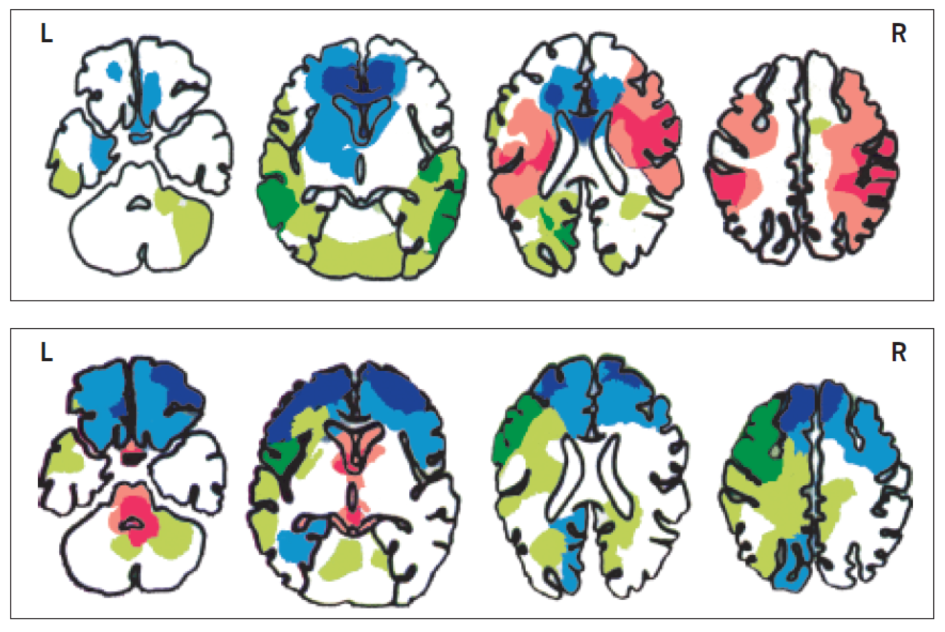
\includegraphics[width=\textwidth]{Fig/Intro/Intro_Lesions/Intro_Lesions.png}
	\caption[Lesion maps associated with cessation vs preservation of dreaming]{Lesion maps associated with cessation vs preservation of dreaming. Top: Global cessation of dreaming was found following parietal lobe lesions (6 cases, inferior lobule and supramarginal gyrus; red), medial frontal lesions (9 cases; blue), and posterior lesions (8 cases; green). Bottom: Preserved dreaming was found following left hemispheric and frontal convexity lesions (15 cases; green), bifrontal lesions (14 cases; blue), and brainstem lesions (17 cases; red). Reproduced from \citet{schwartz_dreaming:_2005}}
	\label{fig:intro:lesions}
\end{figure}

\subsection{A continuum of mentation during sleep}
\label{sec:dream-research:link:continuum}

Based on Solms’s findings, some authors have postulated that instead of relying on REM sleep mechanisms, dreaming might be best described along a \q{continuum} of mentation during sleep, ranging from the hypnagogic reveries typical of sleep onset to florid and vivid dreamlike experiences typical during REM sleep \citep{schwartz_dreaming:_2005}. A brief description of this continuum of mental activities during sleep is reported in Table \ref{tab:intro:continuum}.

% Please add the following required packages to your document preamble:

\begin{table}[htb]
\caption[A continuum of sleep mentation]{A brief description of sleep mentation in their typical order of placement during the sleep cycle. Modified from \citet{de_koninck_sleep_2012}}
\label{tab:intro:continuum}
\resizebox{\textwidth}{!}{%
\begin{tabularx}{\textwidth}{XXX}
\toprule
\textbf{Name}                                                         & \textbf{Description}                                                                          & \textbf{Sleep stage}                         \\ \midrule
Hypnagogic reverie                                                    & Simple images                                                                                 & Sleep onset mentation (N1 or early N2 sleep) \\
Reflections                                                           & Thoughts with no hallucinatory content                                                        & N2 sleep                                     \\
Vivid dreams                                                          & Vivid imagery and sequences, presence of characters, interactions and emotions                & REM and NREM sleep                           \\
Lucid dreams                                                          & The dreamer is conscious of dreaming and can sometimes controls the dream scenario            & REM sleep                                    \\
Nightmares and bad dreams 	  										  & Unpleasant and highly anxiogenic dream. The content of nightmare actually awakens the dreamer & REM sleep                                    \\
Hypnopompic reverie                                                   & Characterized by elaborate imagery                                                            & Sleep offset mentation (REM or NREM sleep)   \\ \bottomrule
\end{tabularx}%
}
\end{table}


\section{Attempts to study the cerebral correlates of dreaming}
\label{sec:dream-research:attempts}

Thanks to the recent advances in neuroimaging techniques, we have the means to measure, with unprecedented spatial and temporal accuracy, what is happening in the brain at a specific moment in time (see Methods section). Yet, since it is now well-accepted that dreaming can occur in all sleep stages, and because dream consciousness is only accessible via report rather than direct observation, it is therefore impossible to be sure that dreaming is happening at a specific time point during sleep. This conceptual issue has not prevented sleep and dream researchers to attempt to identify the cerebral correlates of dreaming. The main methods and findings are summarized in the following paragraphs.

\subsection{Brain activity during REM sleep}
\label{sec:dream-research:attempts:ba-rem}

On the basis of the REM sleep hypothesis of dreaming, which was predominant during the nineties, researchers used functional neuroimaging techniques such as positron emission tomography (PET) to investigate the brain activity during REM sleep. They reported that, despite strong similarities between the wake and REM sleep electrophysiological scalp signals, the brain metabolism in these two vigilance states was disparate \citep{maquet_functional_1996, braun_regional_1997}. Among the most notable findings, the regional cerebral blood flow (rCBF) was decreased in several brain regions including the dorsolateral prefrontal cortex (DLPFC), and was increased in other regions (occipital, temporal, and superior parietal cortices, hippocampal formation, anterior cingulate and the pons). Following these works, researchers postulated that these changes in the brain functional organization could explain the phenomenological characteristics of dream reports \citep{hobson_dreaming_2000, nir_dreaming_2010}. For instance, increased occipital cortex activity during REM sleep could explain the clear predominance of visual modality in dream reports, a phenomenon that Vincent van Gogh had already noticed when he wrote: \q{I often think that the night is more alive and more richly colored than the day} (Vincent van Gogh, 1888). Second, the increased activity during REM sleep in the hippocampal formation, a region well-known for its role in memory encoding and retrieval, could account for the presence of known images and characters in dreams. Finally, the decreased activity in the dorsolateral prefrontal cortex, a region involved in executive function, cognitive control and working memory, could account for the lack of consistency, voluntary control and logical reasoning over the dream story. This is consistent with studies on lucid dreaming which showed a partial reactivation of this area in lucid dreams compared to non-lucid dreams. We will return to these correspondences between the phenomenology of dreams and brain activity in the chapter on the default mode network.

\subsection{Brain activity during lucid dreaming}
\label{sec:dream-research:attempts:ba-lucid}

Long considered as a fantasy, lucid dreaming - the ability to become self-aware of dreaming during a dream, and in some cases, to control the dream scenario – has recently gained considerable interest among researchers and the public. The scientific study of lucid dreaming started in the nineteenth century when Hervey de Saint Denys, a learned oneirologist, published his landmark book \q{Dreams and the Ways to Direct Them: Practical Observations}, in which he described his own lucid dream experiences. More than a century later, more objective methods such as EEG and functional magnetic resonance imaging (fMRI) have become the technique of choice for understanding lucid dreams. Using a pre-determined ocular signal, Dresler was remarkably able to measure, in real-time, the brain activity during lucid REM sleep and non-lucid REM sleep (though only one subject out of four had lucid dreams of sufficient length; \citet{dresler_neural_2012}). Lucid REM sleep was associated with a reactivation of areas that are normally deactivated during REM sleep, such as bilateral precuneous, parietal lobules and prefrontal and occipito-temporal cortices. Phenomenologically, these regions are either involved in self-awareness and executive functions, and their reactivation during lucid dreaming could account for the resurgence of a certain level of self-awareness and voluntary control. Even more recently, Voss was able to induce self-reflective awareness during dream using fronto-temporal transcranial alternating current stimulation \citep{voss_induction_2014}. They reported that lucid dreams were most prominent during stimulation in the lower gamma band (58\% of lucid dreams following a stimulation at 25 Hz and 77\% of lucid dreams following a stimulation at 40 Hz). However, the lucidity was not assessed directly by the dreamer but assumed a posteriori if the subjects reported elevated ratings on a lucidity scale. In conclusion, lucid dreaming provides an appealing and elegant way to study, in real time, the cerebral correlates of dreaming. Yet, the inherent problem with this method lies precisely in the fact that lucid dreams are, by nature, different from non-lucid dreams. As exciting as the results are, it would be however difficult to generalize them to the research on non-lucid dreams.

\subsection{Brain activity in the minutes preceding a dream report}
\label{sec:dream-research:attempts:ba-pre}

Another line of research consists in comparing the EEG power in various frequency bands in the minutes preceding a morning awakening associated, or not, with a dream recall. This paradigm has been used in several studies over the last decades, the findings of which are summarized as follows.

\citet{esposito_reduced_2004} reported that in both REM and N2 sleep, dream recall was associated with a lower alpha and delta power in the 3 minutes preceding awakening. According to the authors, the alpha effect may reflect increased cognitive elaboration and visual imagery as well as increased attention and memory processes. A few years later, \citet{marzano_recalling_2011} found that dream recall after morning awakening from REM sleep was associated with a higher frontal 5–7 Hz (theta) activity in the 5 minutes preceding awakening. In N2 sleep, dream recall was associated with a decrease in alpha power, an observation consistent with Esposito’s results. The same year, another study reported a lower delta power for the dream recall condition following awakening from N2 sleep, and a higher alpha and beta power in occipital derivations for REM sleep \citep{chellappa_cortical_2011}. Finally, a recent study, inaccurately entitled \q{the cerebral correlates of dreaming}, reported that in both N2 and REM sleep, reports of dream experience were associated with local decreases in delta power in posterior cortical regions in the 2 minutes preceding awakening \citep{siclari_neural_2017}. The authors were able to predict whether an individual reported dreaming or the absence of dream experiences after awakening from N2 sleep by monitoring this posterior ‘hot zone’ in real time.
The results from these studies are heterogeneous and sometimes contradictory. Moreover, despite this paradigm may seem attractive at first, the problem still remains that we can never be sure whether the dream actually took place in the minutes just before awakening or several tens of minutes before.

\subsection{Dreaming as a subsystem of the default mode network}
\label{sec:dream-research:attempts:dmn}

The past few years have witnessed the emergence of a new conceptual framework of dreaming, centered on the idea that dreaming is a unique form of mind-wandering, which cerebral correlates are a subsystem of the default mode network (DMN; see Methods section; \citealp{maquet_human_2005, domhoff_neural_2011, domhoff_dreaming_2015, christoff_mind-wandering_2016}). Based on the fact that dreaming and waking spontaneous thought share many features (i.e. predominance of the audiovisual modalities, centered on one’s current goals and concerns, draw heavily on semantic and episodic memory in constructing simulations and future plans, presence of a wide range of affect), some authors have postulated that dreaming is a \q{type of spontaneous thought that is highly unconstrained, hyper-associative and highly immersive} \citep{christoff_mind-wandering_2016}. Using the results of lesion and REM sleep neuroimaging studies, they argued that dreaming should be accompanied, at the neural level, by a strong recruitment of the default mode network medial temporal lobe (MTL)-centered subsystem and strong deactivations in frontoparietal control network regions (such as the DLPFC). Activation of the former areas could be related to the generation of spontaneous thoughts, during both wake and sleep, while the deactivation of the latter areas could explain the high volatility and variability of dream content over time.

\cleardoublepage

\chapter{Dream recall frequency}
\label{sec:dream-recall}

\cleanchapterquote{We must also inquire what the dream is, and from what cause sleepers sometimes dream, and sometimes do not; or whether the truth is that sleepers always dream but do not always remember (their dream); and if this occurs, what its explanation is.}{Aristotle}{On dreams. 350 B.C.}

\section{Measuring dream recall frequency}
\label{sec:dream-recall:method}

As Aristotle had rightly pointed out, we do not always remember our dreams. More than two thousand years after, modern research has confirmed that the dream recall frequency (DRF) – i.e. the number of dream reports over a given period of time - is indeed highly variable both within individuals over the life course, but also between individuals \citep{schredl_factors_2003, ruby_experimental_2011}.

There is no gold standard for measuring DRF, and each method has its pros and cons. In research settings, three methods are commonly applied: questionnaire scales, dream diaries, and laboratory awakenings \citep{schredl_dream_1999}. The former consists in asking the participants to estimate their dream recall frequency over the last few weeks or months. This method has the advantage of being fast, inexpensive, and unaffected by the measurement, however, the DRF could be over- or under-estimated due to erroneous or incomplete recollection. Regarding dream diaries, the participants are asked to report each morning whether they have recalled a dream or not. This method minimizes the bias of retrospective estimation, but has the disadvantages of potentially increasing drastically the dream recall frequency, especially in persons who usually almost never recall their dreams \citep{schredl_questionnaires_2002}. Finally, laboratory awakenings consist in awakening the participants in the sleep lab and asking them whether they recall a dream or not. While this method has the clear advantage that the experimenters can measure physiological parameters (EEG, EOG, ECG, respiration and heart rate) prior, during and after the awakening, it is also time-consuming and expensive. Moreover, as for dream diaries, laboratory awakenings are associated with a dramatic increase in DRF, especially for low dream recallers.

\section{DRF in the general population}
\label{sec:dream-recall:pop}

\subsection{Average DRF}
\label{sec:dream-recall:pop:avg}

Measured by questionnaire, the average weekly DRF was 2.58 ± 2.03 in 444 German students \citep{schredl_factors_2003} and 0.83 ± 1.57 in a representative German sample of 931 participants \citep{schredl_dream_2008}. Using dream diaries, the average weekly DRF was 3.1 ± 1.5 in 70 Finnish children \citep{valli_threat_2005} and 3.9 ± 2.5 in a sample of 196 German student \citep{schredl_reliability_2005}. In lights of these results, we can conclude that the average weekly DRF in the general population lies between 1 and 3 dream reports per week.

\subsection{Intra-individuals variability}
\label{sec:dream-recall:pop:intra}

Daily experience suggest that our ability to recall dream fluctuate over time. Investigating this issue using the diary technique in 169 participants, \citet{schredl_reliability_2005} reported that the stability of DRF was very high over a period of one month. Similarly, he reported high DRF stability coefficients in a sample of older adults who had been interviewed weekly about their dream life over a period of 26 weeks \citep{schredl_reliability_2001}. However, to our knowledge, there are no studies evaluating the stability of DRF in the same individuals over an extended period of time.

\subsection{Inter-individuals variability}
\label{sec:dream-recall:pop:inter}

DRF varies drastically between individuals: some persons almost never recall a dream, whereas others can recall one or several dreams every morning. In an Austrian sample of 1000 persons, \citet{stepansky_austrian_1998} found that 31\% of the participants reported 10 dreams or more per month, 37\% reported between one and nine dreams per month, and 32\% reported less than one dream per month. In a sample of 285 German students, \citet{schredl_questionnaires_2002} found that 44\% reported dreams four or more times per weeks, 44\% reported a dream one time per week and 12\% reported a dream less than one time per month. This variability allows to differentiate behavioral profiles of DRF: high dream recallers (HR), who can recall a dream almost every morning (e.g. more than 5 mornings a week, \citealp{schredl_reliability_2005}) and low dream recallers (LR), who almost never recall a dream (e.g. less than one dream per month, \citealp{goodenough_comparison_1959}). Importantly, the frequency of HR is higher in the general population, and even more in young and/or student sample \citep{schredl_reliability_2005}.

\section{Parameters correlated with DRF}
\label{sec:dream-recall:param}

\subsection{Physiological and psychological factors}
\label{sec:dream-recall:param:psych}

First, increased professional or personal stress is positively associated with DRF \citep{schredl_dream_1999}. Similarly, an interest in dreams, or a positive attitude towards dreams is positively associated with DRF, as is frequent day-dreaming and rich fantasy life \citep{schredl_factors_2003}. DRF decreases with age and is slightly higher in women, who are also typically more interested in dreams \citep{schredl_dream_2008, schredl_gender_2008}. Regarding personality dimensions, studies have found positive correlations between DRF and thin boundaries, anxiety, and openness to experience \citep{hartmann_boundaries_1989, schredl_factors_2003,schredl_dream_2003}. However, most of the correlations between DRF and personality traits are low and explain only a small percentage of the total variance.

\subsection{Cognitive factors}
\label{sec:dream-recall:param:cogn}

Regarding cognitive abilities, a simple explanation of why individuals differ in their ability to remember dreams could be because they differ in some more general memory abilities (verbal, visual, short and long term). However, the literature yielded contradictory results, with some support for a positive association between DRF and visual memory, but also evidence against it for verbal and visual material and short-or long-term story narrative recall \citep{ruby_experimental_2011, blagrove_trait_2010}. On another note, several studies have consistently reported that DRF is positively correlated with creativity \citep{fitch_variations_1989, schredl_creativity_1995, schredl_factors_2003} and intelligence scales (multiple-choice vocabulary test, \citealp{schonbar_manifest_1959}, Shipley-Hartford intelligence scale, \citealp{connor_reported_1970}).

\subsection{Sleep parameters}
\label{sec:dream-recall:param:sleep}

First, DRF varies according to the sleep stage preceding awakening (see \citealp{nielsen_review_2000} for a review). More dream reports are obtained after an awakening during REM sleep than after an awakening during NREM sleep. These results inspired the REM sleep hypothesis of dreaming discussed earlier in section \ref{sec:dream-research:link:rem-sleep}. However, when a dream is not reported on awakening, there is no method of establishing whether it did not happen or was forgotten. This idea was rightly pointed out by \citet{conduit_poor_2004}: \q{An ongoing assumption made by sleep scientists is that since dreams are more often recalled on awakening from REM sleep, dreams must occur more often during this sleep stage. An alternative hypothesis is that cognition occurs throughout sleep, but the recall of mentation differs on awakenings}.

This idea that DRF variability is not a matter of dream production during sleep, but of dream recall during awakening, is the core of several models of dream recall (detailed later in section \ref{sec:dream-recall:theories}), among which the arousal-retrieval model is one of the most significant. In its simplest form, it claims that a period of wakefulness must occur just after dreaming so that the dream content can be transferred from short term to long term memory \citep{koulack_dream_1976}
Several studies support this model. First, using retrospective evaluation, \citet{schredl_factors_2003} found a positive correlation between the number of nocturnal awakenings and DRF. Second, \citet{de_gennaro_recovery_2010} reported that recovery sleep following a full night of sleep deprivation was characterized by an almost complete abolition of dream recall, paralleled with a lower number of nocturnal awakenings, which could, according to them, have \q{reduced the contents available in memory as possible cues for retrieval of dream experiences at morning}. Finally, these results were recently reinforced by a full-night PSG study in 36 subjects (18 HR and 18 LR; \citealp{eichenlaub_brain_2014}; Figure \ref{fig:intro:jbe-sleep}). HR showed in average longer intra-sleep wakefulness than LR (30 min vs 15 on average). The number of awakenings (the number of phases composed of consecutive pages of awakening) was not significantly different between the 2 groups, but the mean duration of the awakenings was (HR, 1.90 ± 0.91 min; LR, 0.95 ± 0.40 min).

\begin{figure}[htb]
	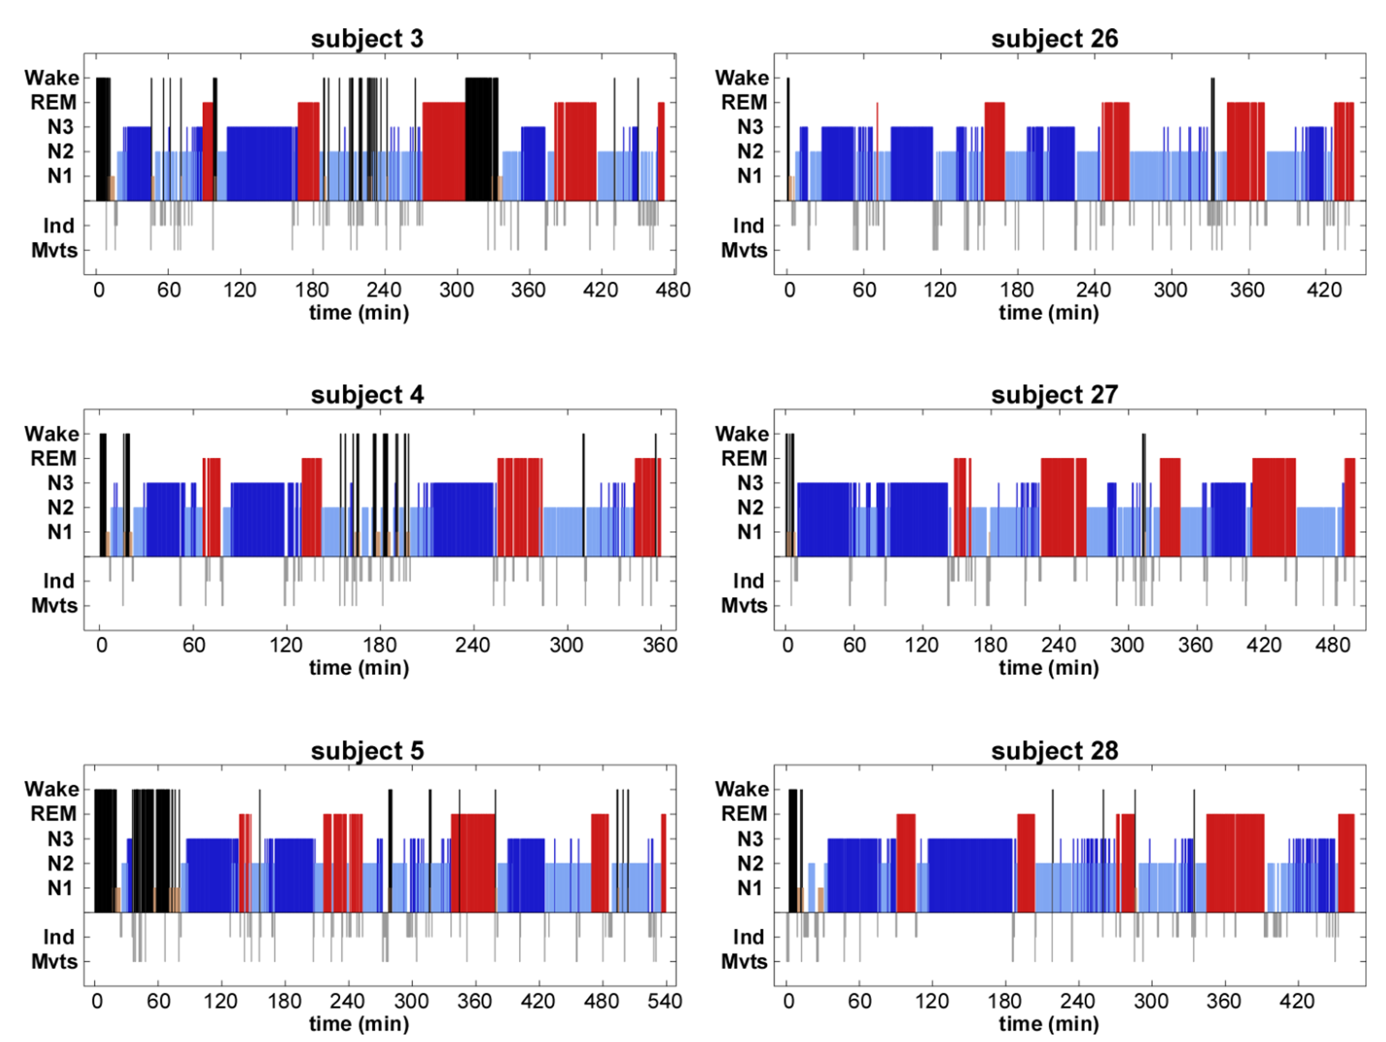
\includegraphics[width=\textwidth]{Fig/Intro/Intro_JBE_sleep/Intro_JBE_sleep.png}
	\caption[Hypnograms of typical high and low dream recallers]{\textbf{Hypnograms of three representative HR (left) and three representative LR (right).} Full night PSG recordings were acquired in the sleep lab in 18 HRs and 18 LRs. Wake: wakefulness (black); N1, N2, and N3: sleep stages N1 (very light gray), N2 (light gray), and N3 (dark gray), respectively; REM: REM sleep (medium gray); Ind: pages for which the dominant sleep stage could not be determined; Mvts: movements. From these 6 examples, it can be observed that the wakefulness periods during the sleep period time are longer in HR than in LR. Adapted from \citet{eichenlaub_brain_2014}}
	\label{fig:intro:jbe-sleep}
\end{figure}

\subsection{Neurophysiological parameters}
\label{sec:dream-recall:param:neuro}

The neurophysiological parameters that covary with DRF had never been investigated until the doctoral work of Jean-Baptiste Eichenlaub, conducted with Perrine Ruby a few years ago. They compared the brain activity of HR and LR during both sleep and wakefulness and using several neuroimaging techniques such as auditory evoked potentials (AEP) and positron emission tomography (PET). The main findings from Eichenlaub’s doctoral thesis are summarized in Figure \ref{fig:intro:jbe-summary}.
First, they conducted a sleep lab study in which they compared the brain reactivity (AEP) of 18 HRs (DRF = 4.4 ± 1.0 dream reports per week) and 18 LRs (0.25 ± 0.1) during sleep and wakefulness \citep{ruby_alpha_2013, eichenlaub_brain_2014}. During data acquisition, the subjects were presented with sounds to be ignored (first names randomly presented among pure tones) while they were watching a silent movie or sleeping. They found that brain responses to first names dramatically differed between the 2 groups during both sleep and wakefulness (Figure \ref{fig:intro:jbe-summary}A). During wakefulness, the attention-orienting brain response (P3a) and a late parietal response were larger in HR than in LR. During sleep, there were between-group differences at the latency of the P3a during N2 sleep and at later latencies during all sleep stages.
Second, they used PET to compare the resting state cerebral blood flow of 21 HRs (DRF = 5.2 ± 1.4 dream reports per week) and 20 LRs (DRF = 0.5 ± 0.3 dream reports per week) during sleep and wakefulness \citep{eichenlaub_resting_2014}. Compared with LRs, HRs showed higher rCBF in the TPJ during REM sleep, N3, and wakefulness, and in the MPFC during REM sleep and wakefulness (Figure \ref{fig:intro:jbe-summary}B).
Altogether, these findings show that HR and LR have different neurophysiological traits: spontaneous and evoked brain activity of HR and LR differ during wakefulness and sleep. They argued that HR’s neurophysiological profile could promote mental imagery during sleep and the encoding or retrieval of the dream memory during wakefulness. Notably, increased attention-orienting responses during sleep in HR could promote intra-sleep awakenings, which in turn would facilitate the encoding of dreams according to the arousal-retrieval model, and finally result in a higher likelihood of dream recall in the morning after awakening.

\begin{figure}[!htb]
	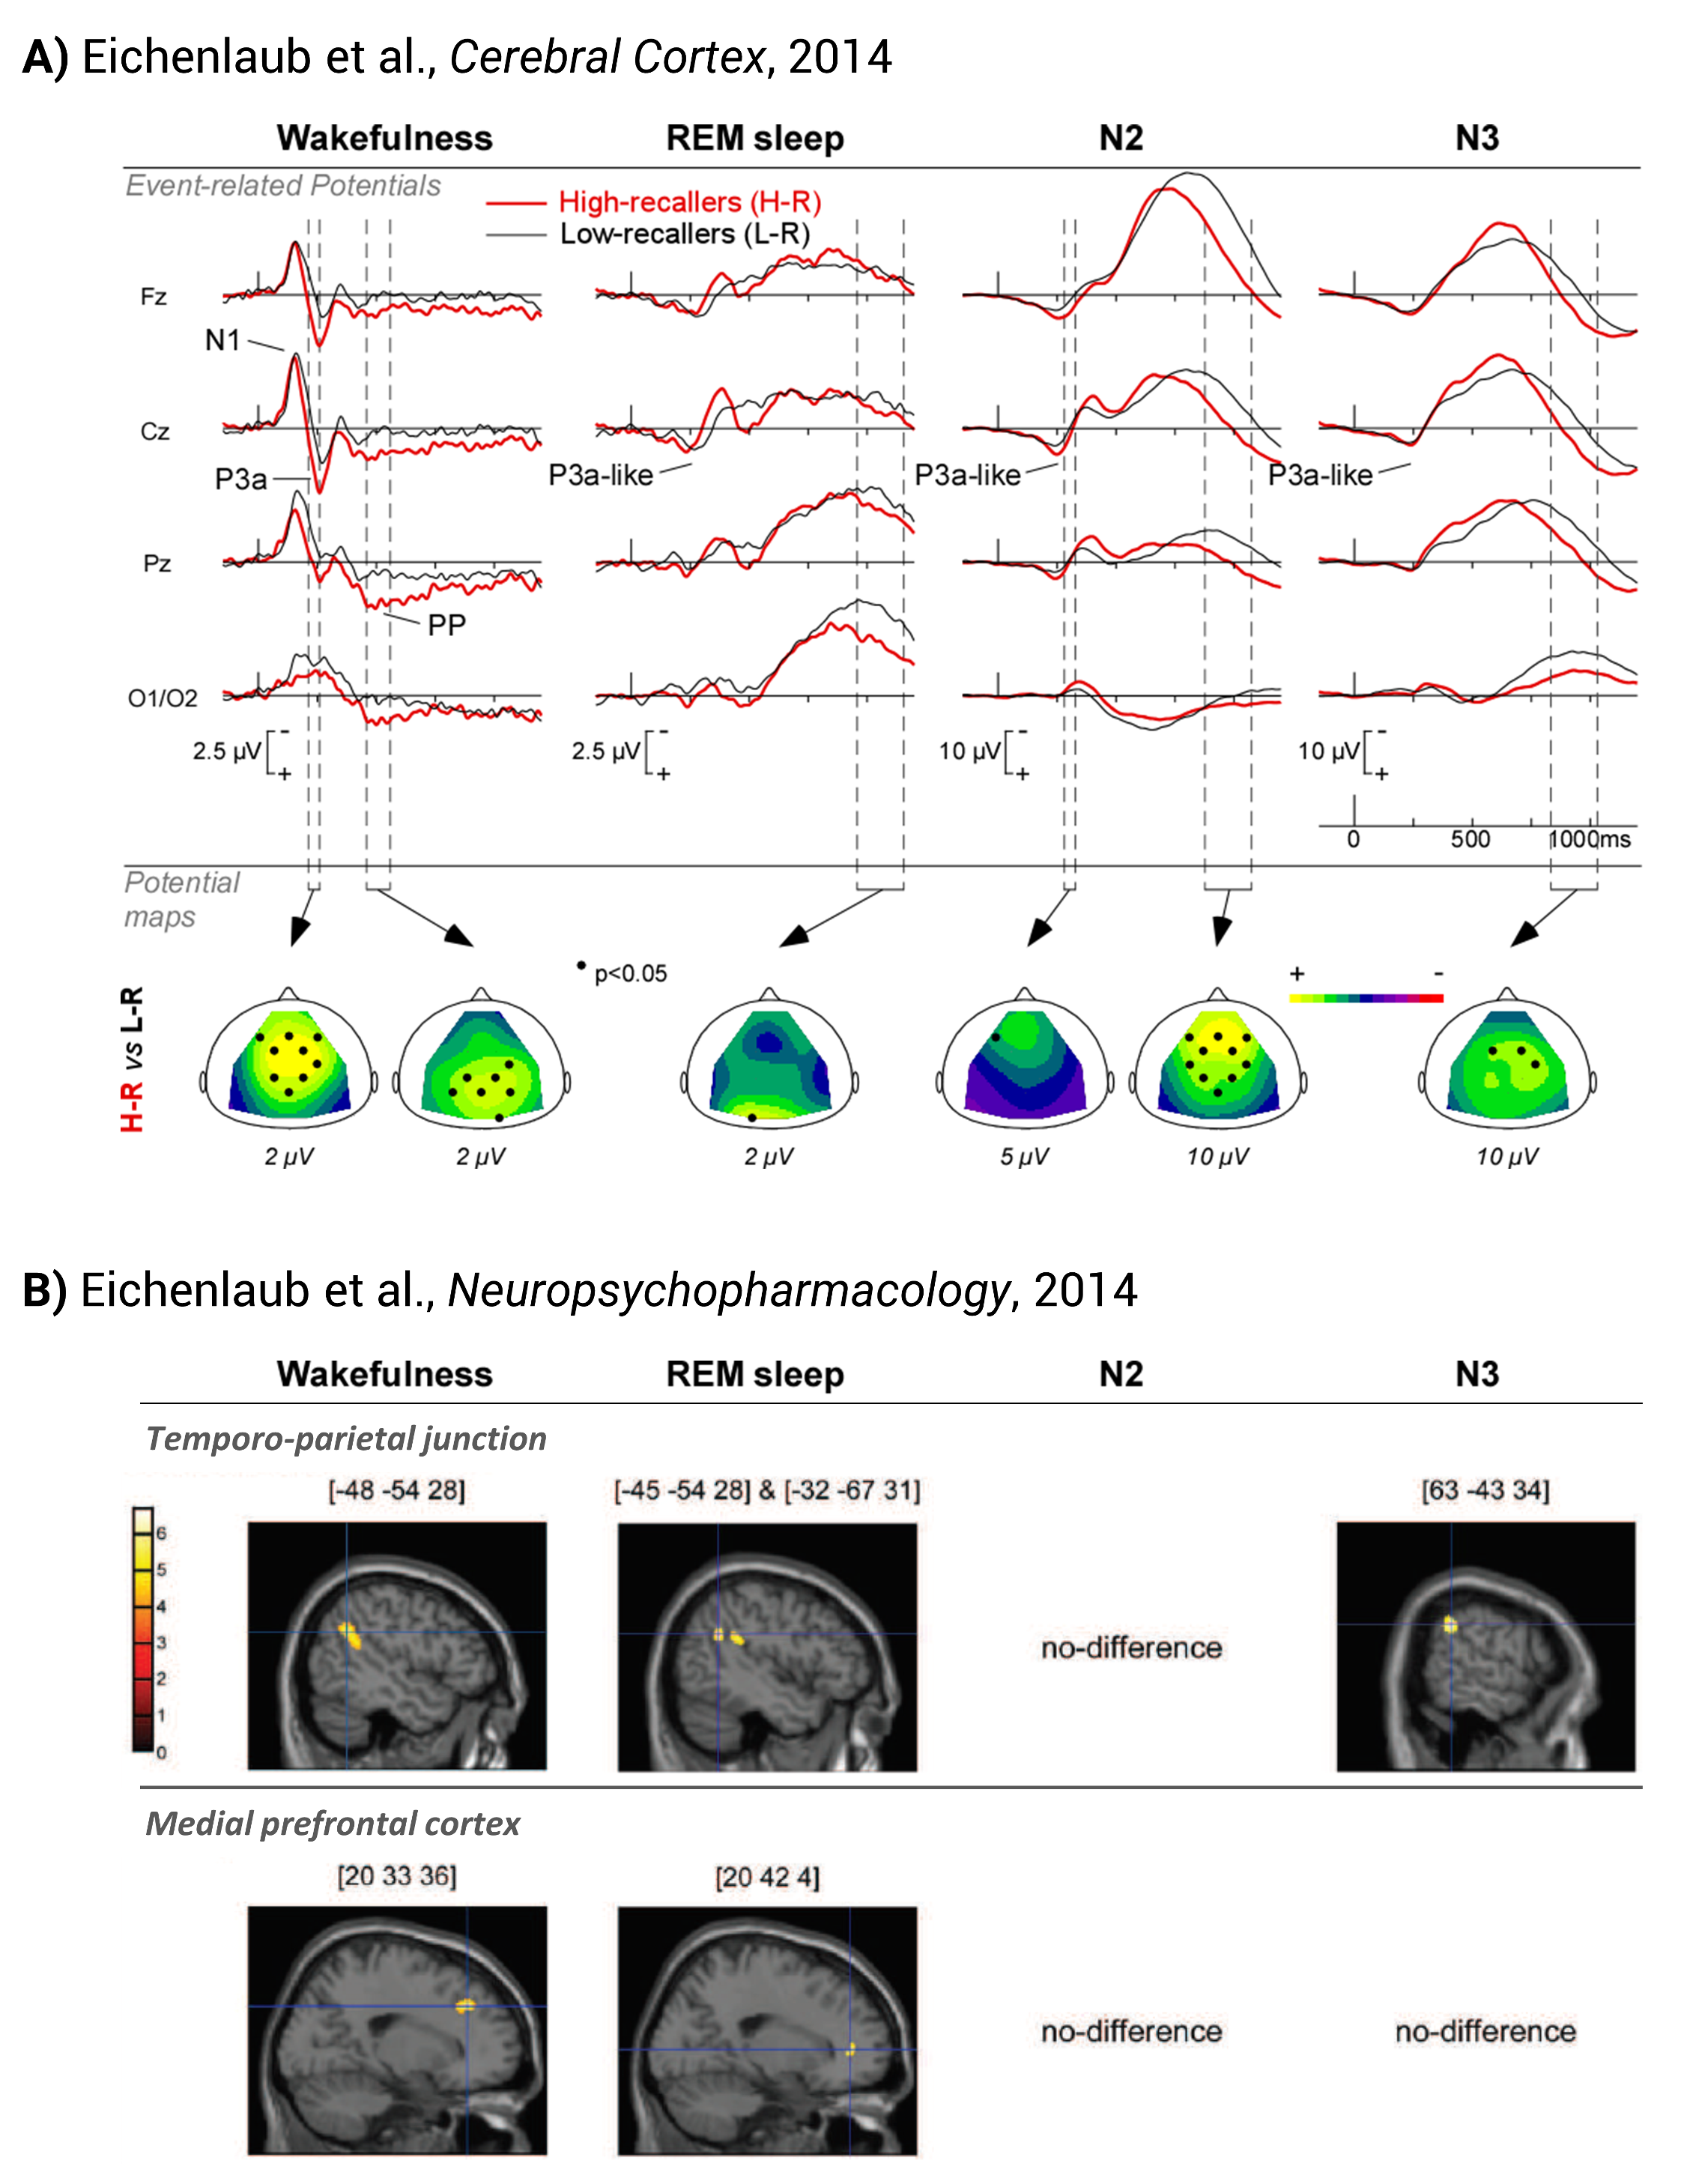
\includegraphics[width=\textwidth]{Fig/Intro/Intro_JBE_summary/Intro_JBE_summary.png}
	\caption[Summary of the results obtained in Eichenlaub's PhD thesis]{\textbf{Summary of the results obtained in Eichenlaub's PhD thesis.} \emph{Top}. EEG study. Compared to LR, HR showed larger brain responses to auditory stimuli (first names) during wakefulness, REM sleep, N2 sleep and N3 sleep. \emph{Bottom}. PET study. Compared to LR, HR showed increased spontaneous rCBF in the TPJ during wakefulness, REM sleep and N3 sleep, and in the MPFC during wakefulness and REM sleep. Altogether, these findings show spontaneous and evoked brain activity of HR and LR differ during both wakefulness and sleep, thus suggesting that DRF is associated with a specific brain functional organization.}
	\label{fig:intro:jbe-summary}
\end{figure}

\subsection{Link between neurophysiological and psychological traits}
\label{sec:dream-recall:param:link}

In conclusion, we have seen that many parameters covary with DRF. The ability to recall dreams seems to be associated with psychological and personality factors on one hand, and neurophysiological trait factors on the other hand. These results should be regarded as complementary. For instance, the fact that HRs demonstrate higher rCBF during sleep and wakefulness in the TPJ and MPFC, two regions of the DMN, is consistent with the DMN hypothesis of dreaming, and is well in line with the finding that HRs are more often absorbed in their inner worlds (i.e. day-dreaming, fantasy) and more anxious. Indeed, studies have reported a positive correlation between the activity of the MPFC during wakefulness and scores of openness to experience \citep{sutin_sex_2009} and neuroticism \citep{zald_brain_2002}.

\section{Theories on dream recall}
\label{sec:dream-recall:theories}

This section summarizes the main theories to explain variability in DRF (see also \citealp{schredl_dream_1996}).

\subsection{Freud’s repression hypothesis}
\label{sec:dream-recall:theories:freud}

Freud believed that the function of dreams is to preserve sleep by representing as fulfilled wishes that would otherwise awaken the dreamer. According to him, \q{the forgetting of the dream is in a large measure the work of the resistance} \citep{freud_interpretation_1900}, which means that dreams that are not sufficiently disguised to pass the censor will be entirely repressed and therefore forgotten. However, as highlighted by \citet{schredl_dream_1999}, it is currently impossible to test this hypothesis because we cannot access the non-recalled dreams in order to compare them to the recalled ones.

\subsection{Life-style hypothesis}
\label{sec:dream-recall:theories:life-style}

Schonbar was one of the first to investigate the psychological correlates of differential DRF. She proposed that DRF can be better explained as part of a general life-style and personality traits \citep{schonbar_differential_1965}. According to her work, high dream recallers are characterized by an ‘inner-acceptant’ life-style, which involves higher creativity, introspection, fantasy proneness and openness to experience. This hypothesis has been corroborated by several experimental studies that reported a positive association between DRF on one hand and openness to experience, absorption and creativity on the other hand (see section \ref{sec:dream-recall:param:link}).

\subsection{Salience hypothesis}
\label{sec:dream-recall:theories:salience}

Based on the idea that the principles of waking memory apply to dream recall, Cohen developed in the seventies the interference hypothesis \citep{cohen_dream_1973} followed by the salience hypothesis \citep{cohen_test_1974}. The interference hypothesis postulates that the dream memory trace remains so long as there is no distraction or interference. Otherwise, dreams are forgotten in order to maximize the memory capacity for the day ahead. This echoes French philosopher Roger Caillois’s idea on dream forgetting: \q{Dreams are quickly forgotten because they have no consequences on waking life and there is only benefits in forgetting them} \citep{caillois_incertitude_1956}. In more practical terms, the central idea of this theory is that the dreamer must voluntary pay attention to the dream immediately after awakening. In this respect, it overlaps the life-style hypothesis since high dream recallers are expected to be more interested in their dreams and therefore put more attention on them upon awakening.
Cohen further extended his model in the salience hypothesis, which states that the more salient a dream (e.g. a vivid, bizarre, and highly emotional dream content), and the less interferences there are during the recall process, the more likely the dream is to be recalled. Several findings are in favor of this hypothesis. For example, it has been shown that bizarreness \citep{cipolli_bizarreness_1993} and emotionality \citep{schredl_emotions_1998} enhance recall of dream content (an observation that was however not replicated when taking the effect of dream length into account; \citealp{schredl_relationship_2000}). More recently, \citet{parke_re-examination_2009} have studied the combined effect of interference and salience processes on dream recall. The findings suggest that a link is present, as the more interference experienced has tended to reduce the length of the dream recall in turn reducing the reported salience.

\subsection{Arousal-retrieval model}
\label{sec:dream-recall:theories:arousal}

\citet{koulack_dream_1976} proposed in their so-called arousal-retrieval model that a short period of wakefulness (arousal\footnote{\citet{koulack_dream_1976} used the word \emph{arousal} to describe a short period of wakefulness, without explicitly mentioning a minimum and maximum duration. To avoid ambiguity, it should be noted that the word \emph{arousal}, as it is used in the present thesis, refers to short events (typically 3 to 15 seconds) that are scored independently of the sleep stages and are therefore different from full (> 15 sec) awakenings; for more details see \ref{sec:problematic:arousals}}) must occur immediately after dreaming in order to transfer the dream content from short-term memory to long term memory. Furthermore, they drew on Cohen’s work to propose that the salience of dream content and lack of interferences during the recall process were critical for a successful recall of the stored dream (retrieval). The arousal-retrieval model is one of the most comprehensive model of dream recall and has received great support from the literature, reviewed earlier in section \ref{sec:dream-recall:param:sleep}.

\subsection{State-shift hypothesis}
\label{sec:dream-recall:theories:state}

Extending these arousal-based ideas, \citet{koukkou_dreaming:_1983} proposed the state-shift hypothesis which emphasizes the state dependent effects of dream recall rather than short-term memory effects. According to them, \q{forgetting of dreams is a function of the magnitude of the difference between states during encoding and recall} \citep{koukkou_dreaming:_1983}. Consequently, the closer two functional states are, the better is the transference of information. Thus, according to them, dreams are better recalled when the awake functional state
is similar to the sleeping functional state. It was argued that such compatibility occurs between wakefulness and REM sleep, enabling better recall of REM dreams. By contrast, the slow EEG frequencies of NREM sleep (and especially N3 sleep) are functionally very different from wakefulness, and this could account for the poorer NREM dream recall.

\subsection{Sleep inertia}
\label{sec:dream-recall:theories:inertia}

\citet{conduit_poor_2004} demonstrated that the cognitive performance during or shortly after awakening is of importance for the process of dream recall. The design of their study is as follows. Participants were instructed to produce an eye movement signal whenever they heard a tone, presented at increasing volume during N2 and REM sleep until an eye movement signal verification was observed.  Ninety seconds after signal verification, participants were awakened and asked if they remembered hearing the tone or responding with the EM signal. Such recollection of signal verified tone presentations was significantly less after Stage 2 sleep (65\%) compared to REM sleep (100\%) presentations. Furthermore, signal verified tone recall was significantly correlated with reported dream recall frequency. They concluded that \q{quite possibly, brain functioning underlying the reporting and non-reporting of dreams does not exist within the pre-sleeping period at all, but within the period just after awakening, when cognitive resources are in demand to recall and/or consolidate events which have just occurred within the previous sleeping period} \citep{conduit_poor_2004}.
Echoing these findings, \citet{schredl_factors_2003} noted that cognitive functioning in the period just after awakening is often severely impaired (an effect referred to as sleep inertia; \citealp{tassi_sleep_2000, trotti_waking_2016}), and that it would be in consequence \q{promising to correlate inter-individual differences regarding the sleep inertia with DRF}. This issue will form a large part of the doctoral work hereby presented and we will return to this in section \ref{sec:problematic:inertia}.

\subsection{Towards a unifying theory of dream recall}
\label{sec:dream-recall:theories:unifying}

This brief overview leads to the observation that there is a broad spectrum of dream recall theories, ranging from relating to the content of the dream (Freud’s repression and Cohen’s salience hypotheses) to accounting for the psychological (life-style hypothesis), cognitive and physiological processes (arousal-retrieval,  state-shift hypothesis, sleep inertia; see Figure \ref{fig:intro:dream-recall-models}). The empirical data seems hitherto to fit best into the arousal-retrieval model (which integrates elements of both the Salience and Interference hypotheses) and the life-style hypothesis. A comprehensive, unified theory of dream recall should combine these two models, for example using the arousal-retrieval model to account for day-to-day variability in DRF (state factors), and the life-style hypothesis to account for the large inter-individual DRF variability (traits factors). Moreover, there is a currently a lack of evidence for the state-shift hypothesis (due to the difficulty of deriving valid quantitative measures for the closeness of functional states; \citealp{schredl_dream_1999}) and the sleep inertia theory, which both insist on brain functioning within the period just after awakening.

\begin{figure}[!htb]
	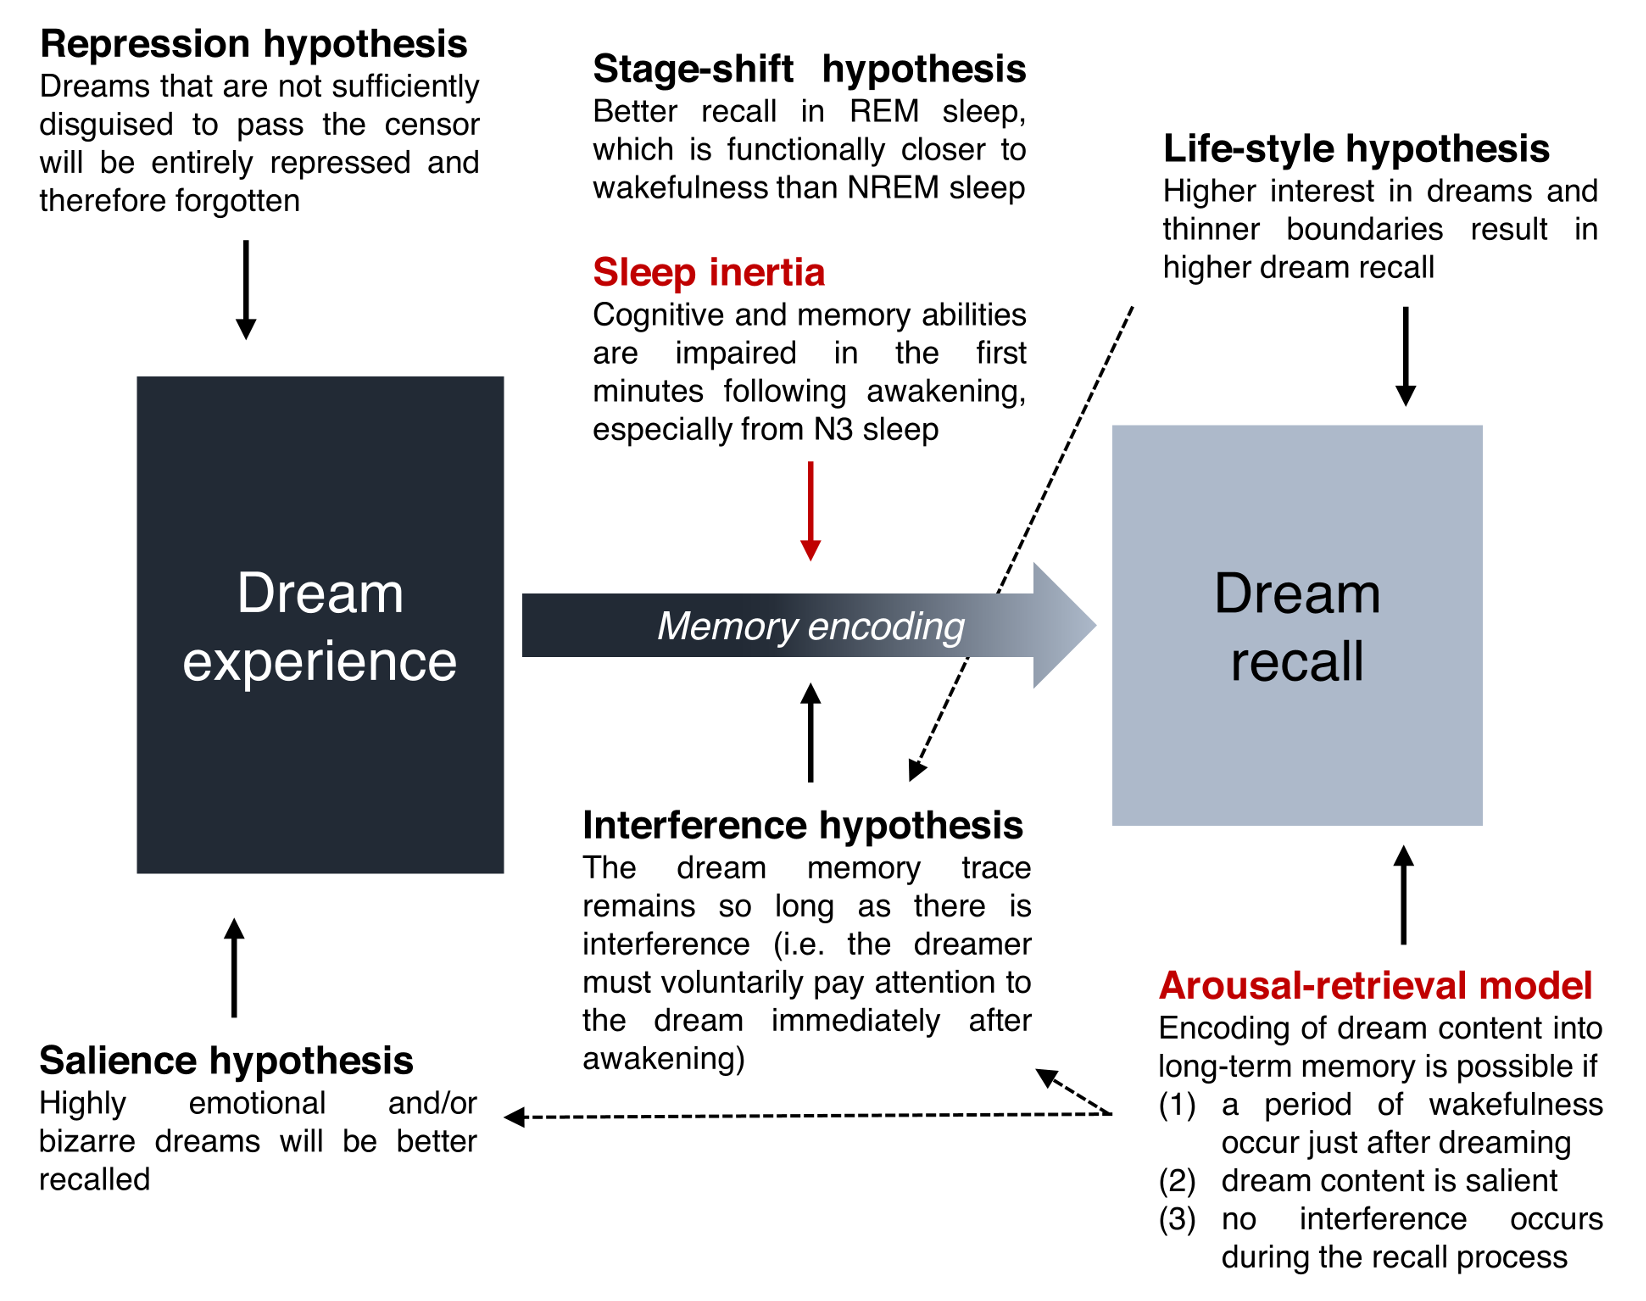
\includegraphics[width=\textwidth]{Fig/Intro/Intro_DRF_model/Intro_DRF_model.png}
	\caption[Dream recall theories]{\textbf{Dream recall theories.} The arousal-retrieval model provides so far the most comprehensive theory on dream recall and is firmly grounded in empirical evidence. At its simplest, it states that a short period of wakefulness must occur just after dreaming (arousal) in order to transfer the dream content from short to long term memory, which is otherwise impossible during sleep. In addition, it postulates that the dream content must be salient (Salience hypothesis, e.g. highly emotional, vivid and/or bizarre) and that the dreamer must voluntarily pay attention to the dream content (Interference hypothesis). Notably, it is very probable that the individuals with the greatest interest in dreams (Life-style hypothesis) are also the ones which focus the more on their dreams immediately after awakening, thus reducing encoding interferences. This would provide a link between the Life-style hypothesis and the arousal-retrieval model. Finally, sleep inertia could be a important explanatory factor with regards to DRF. It is possible that low dream recallers experience more acute sleep inertia upon awakening, whatever the sleep stage before awakening. More impaired memory and cognitive abilities upon awakening would in turn prevent the encoding of dreams to long term-memory. However, this hypothesis remains to be tested empirically.}
	\label{fig:intro:dream-recall-models}
\end{figure}

\cleardoublepage

\chapter{Dream content}
\label{sec:dream-content}

\cleanchapterquote{Prétendre donner les rêves comme de simples jeux de la pensée, de simples images de l’imagination, c’est témoigner d’un manque de réflexion ou de loyauté ; car de toute évidence ils en diffèrent spécifiquement. Les images de l’imagination sont faibles, languissantes, incomplètes, partielles et si fugitives qu’on peut à peine fixer dans sa mémoire pendant quelques secondes les traits d’un absent, et que même le jeu le plus vif de l’imagination ne peut nullement entrer en comparaison avec la réalité palpable que le rêve met sous nos yeux.}{Schopenhauer}{Parerga und Paralipomena, 1851}

\section{Basic principles of dream content analysis}
\label{sec:dream-content:method}

Empirical investigation on dreaming started in the nineteenth century when amateur researchers started to quantify aspects of their dream content. One notable example is the pioneering paper of Mary Calkins \citeyearpar{calkins_statistics_1893}, entitled \q{Statistics of dreams}, in which she reported, inter alia, statistics concerning dream length and vividness, dream characters and dream- and waking-life associations. Since then, a considerable numbers of scales and rating systems for dream content analysis have been developed \citep{schredl_dream_2010}. Most of them are based on automatic analysis of the lexical content of dream reports, a method which has the advantages of minimizing the experimenter bias and being replicable by other research groups. Perhaps the most famous is the Hall \& Van de Castle system, which have provided a global profile of dream content dimensions in young adult \citep{hall_content_1966}. It remains today the major reference since it has proven stable over at least one generation \citep{hall_dreams_1982}.

\section{Quantitative results}
\label{sec:dream-content:quant}

Results from several decades of dream content studies \citep{hall_content_1966, schwartz_exploration_1999, schredl_characteristics_2010} indicate that: dreams tend to be negative on many dimensions and aggressions are more frequent than friendly interactions, visual imagery occurs more frequently in dreams than imagery of other senses (audition, olfaction, touch, and taste); the dream drama is mostly lived by the dreamer from a first-person perspective; some elements of real-life events previously experienced by the dreamer often contribute to the scene of the dream; most often, the dream sequence is not within the dreamer’s voluntary control (i.e., the dreamer may be convinced during the dream that the dream’s story is really happening); temporal and spatial incoherencies can occur in the dream story; the dream report is often full of people interacting with each other (e.g., discussions, fights, pursuit, sexuality); and finally, the dream report often contains strong emotions.
Gender differences in dream content have been consistently reported. For example, men report more often physical aggression and sex than women \citep{nielsen_typical_2003, schredl_typical_2004}.
Finally, many aspects of the subject’s daily life influence dream content (reviewed in \citealp{ruby_experimental_2011}), including news event, musical practice, current concerns and religious beliefs, chronic pain, mood or living in a violent environment.

\section{The sources of dream content}
\label{sec:dream-content:sources}

Based on these experimental findings, \citet{de_koninck_sleep_2012} has reviewed in his book entitled \q{Sleep, dreams and dreaming} the sources that mediate dream construction, as well as their relative contribution to the dream content. He proposed that the different sources of dreams are best represented in a pyramidal manner, from low, more biological levels, predominant in shaping the dream content, to higher, more cognitive levels, that carry much less influence to the dream content (Figure \ref{fig:intro:koninck}).

\begin{figure}[htb]
	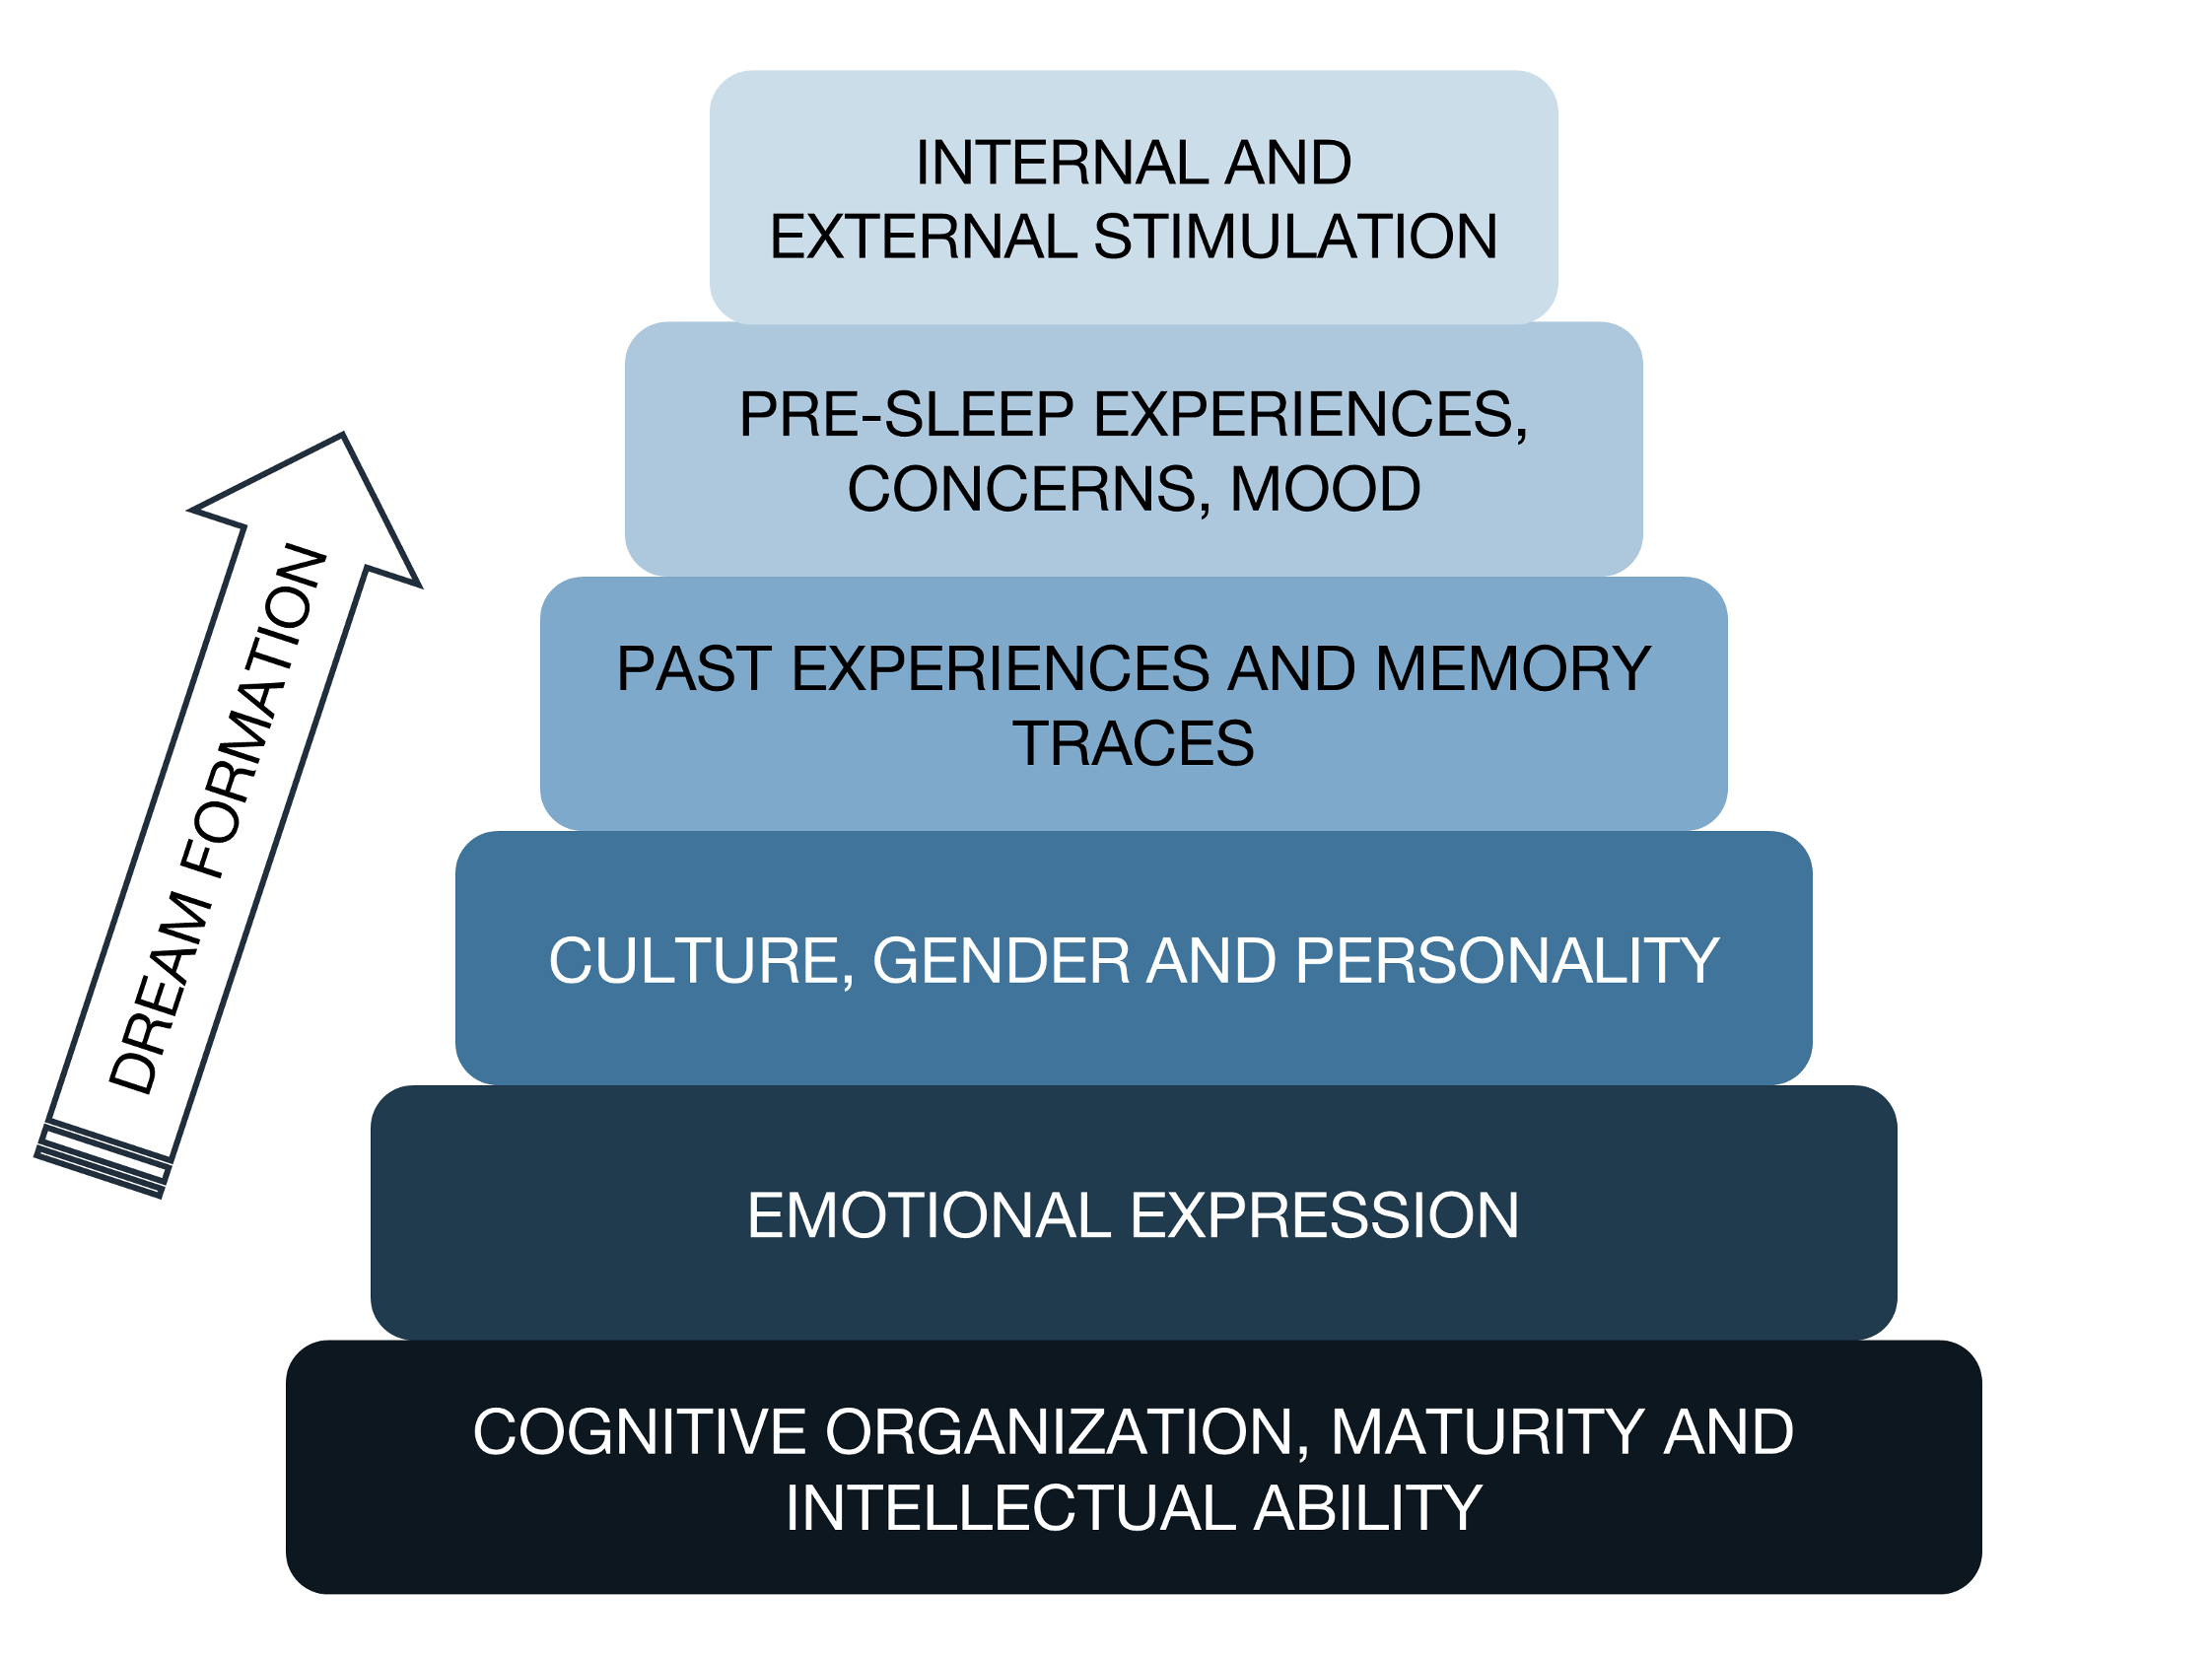
\includegraphics[width=\textwidth]{Fig/Intro/Intro_Pyramid_dream_construction/Intro_pyramid_dream.png}
	\caption[Layers in the construction of dreams]{Layers in the construction of dreams \citep{de_koninck_sleep_2012}. The various factors in the elaboration of dreaming are illustrated as a pyramid suggesting their order and importance.}
	\label{fig:intro:koninck}
\end{figure}

\subsection{The memory sources of dream content}
\label{sec:dream-content:sources:memory}

As we mentioned earlier, there is ample evidence that waking experience finds its way into dreams. However, the characteristics and time course of the waking memory sources integrated into dreams are still unclear. For instance, it is now clear that dream content very rarely replays an episodic memory as it is remembered \citep{fosse_dreaming_2003, nielsen_what_2005}, although it is often related to some elements of the waking life of the dreamer \citep{schredl_characteristics_2010, blagrove_trait_2010, ruby_experimental_2011}. This observation has led to the so-called \q{continuity hypothesis of dreaming} which simply states that dreams reflect waking life experiences \citep{schredl_continuity_2003}.

Several factors have been positively associated with the likelihood of a waking life experience to be incorporated into dreams \citep{schredl_characteristics_2010}. These factors are reviewed in the following lines. First, there seems to be a linear decrease in temporal references identified in dreams, with recent experiences being more incorporated into dreams than older ones \citep{botman_dream_1990, strauch_dem_2004, grenier_temporal_2005}. This finding supports the notion of continuity between waking and dreaming memory processes. Furthermore, several studies \citep{botman_dream_1990, nielsen_day-residue_1992, marquardt_empirical_1996} have confirmed that a significant proportion of dreams contain elements that refer to experiences of the preceding day, a phenomenon known as day-residues and mentioned by Freud who considered them as \q{a necessary ingredient in dream formation} \citep{freud_interpretation_1900}. Another interesting finding is that contrary to what would be expected according to memory decay with time, some studies reported an overrepresentation in dreams of waking experiences that happened approximately one week before the dream \citep{nielsen_day-residue_1992, marquardt_empirical_1996}, however this effect was found only for REM dreams and not N2 or N3 dreams \citep{blagrove_assessing_2011, van_rijn_dream-lag_2015}. Second, there is a preferential incorporation of emotional waking-life experiences into dreams \citep{malinowski_evidence_2014, schredl_factors_2006}. Interestingly, emotional intensity, but not emotional tone seems to affect the incorporation into subsequent dreams. Third, all waking life activities are not represented in the same proportion in dreams \citep{hartmann_we_1996, schredl_continuity_2000}. Focused thinking activity (such as using a computer, reading) are rarely reported in dreams, an effect that may be explained by the generally low emotional intensity of these types of activities. Fourth, the magnitude of the continuity between waking and dreaming is related to some extent to the personality traits of the dreamer \citep{schredl_dreaming_1996}. Finally, chronobiological factors, such as sleep cycles and time of the night, influence dream content. For example, dream reports from the first part of the night comprise more elements of the previous day than dream reports from the second part of the night \citep{roffwarg_effects_1978}.

\cleardoublepage

\chapter{Dream function}
\label{sec:dream-function}

\cleanchapterquote{J’ai rêvé tant et plus, mais je n’y entends note}{François Rabelais}{Pantagruel, 1532}

\section{Historical perspective}
\label{sec:dream-func:history}

\subsection{Ancient and classical history}
\label{sec:dream-func:history:ancient}

Since the dawn of times, humans have tried to assign meaning to their dreams. In many ancient civilizations, dreams were considered as omens or messages from deities, and needed therefore to be correctly interpreted. Numerous examples of dreams sent by Gods can be found in Mesopotamian, Egyptian and Greek mythological narratives, as well as in the sacred books of the three main monotheistic religions (see \citealp{de_koninck_sleep_2012}). Greek philosophers, however were the first to consider dreaming as a natural phenomenon. They provided different explanations of the nature and meaning of dreams, some of which are well in tune with modern dream research. For example, anticipating the notion of continuity between waking and dreaming, Cicero and Herodotus believed that dreams are produced by thoughts, concerns and conversations a dreamer had during the preceding days. Plato on the contrary viewed dreams as the expression of hidden desires and intolerable behaviors, an idea consistent with Freud’s repression hypothesis. Finally, Aristotle thought that dreams were caused by external and internal bodily sensations, an idea consistent with Hobson’s stochastic theory of dream generation.

\subsection{The royal road to the unconscious}
\label{sec:dream-func:history:psychanalysis}

The father of psychanalysis viewed dreams as the \q{royal road to the unconscious} \citep{freud_interpretation_1900}. He defined the unconscious as a part of our mind made up of thoughts, desires, emotions, and knowledge that we are unaware of, but that nevertheless profoundly influence and guide our behaviors. Freud believed that the ego’s defenses are lowered during dreaming, which allows the unconscious mind and the repressed material (i.e. hidden desires) it conveys to come through awareness, albeit in a distorted form. For him, the dream is formed of the manifest content (i.e. the dream as the dreamer recalls it), which is often based on mundane and insignificant day-residues, and the latent content (i.e. symbolic meaning of the dream). The latent content of the dream can be translated into manifest content (a process referred to as dream work) in order to unravel the underlying wish and hidden desires present within the dream. Therefore, in Freud’s model, the dream need to be explicitly remembered and interpreted to possess an adaptive value. It is noteworthy that his hypothesis \q{has rarely been considered by neuroscientists who often consider Freud’s work and theory unscientific} \citep{ruby_experimental_2011}.

\subsection{Psychological individualism}
\label{sec:dream-func:history:jouvet}

Michel Jouvet, one of the pioneers of sleep research, co-discoverer of REM sleep, was also greatly interested in dreams. He kept a dream diary for years, which he used to describe several quantitative measures on dream content. For instance, he was one of the first to report high residue frequencies in dreams approximatively one week days the waking experience (i.e. the dream-lag effect; \citealp{jouvet_memoire_1979}). Regarding the function of dreams, which he equated at the time to the function of REM sleep, he proposed that it is a kind of iterative neurological programming which aims at preserving the expression of the genetic program that codes for psychological characteristics. According to him, this process would ensure the stability of personality across time \citep{jouvet_sommeil_1991}.

\section{Modern theories}
\label{sec:dream-func:modern}

\subsection{An epiphenomenom of REM sleep}
\label{sec:dream-func:modern:nofunc}

Based on the neurophysiological properties of REM sleep, which he equated with dreaming, Alan Hobson proposed that dreaming is an epiphenomenon of REM sleep \citep{hobson_dream_1998}. According to him, the dream imagery is the result of cortical centers trying to create meaning from brainstem-driven signals generated during REM sleep (the so-called activation-synthesis model). In this theory, the dream content is therefore stochastic and is very unlikely to represent an adaptive advantage. It should be noted, however, as noticed by \citet{windt_dreaming:_2015}, that \q{Hobson does not deny that dreams can have meaning and can reflect the personality and concerns of the dreamer. He just thinks that their meaning is transparent and immediately obvious to the dreamer, rather than requiring an elaborate process of interpretation.}

\subsection{Threat / Social simulation theory}
\label{sec:dream-func:modern:revonsuo}

\citet{revonsuo_reinterpretation_2000} proposed that dreaming is a virtual reality in which the dreamer can simulate threatening events and therefore be better prepared to face upcoming dangers in waking life (the so-called threat simulation theory, TST). According to him, \q{dream consciousness is essentially an ancient biological defense mechanism, evolutionarily selected for its capacity to repeatedly simulate threatening events} \citep{valli_threat_2005}. As such, dream content is more consistent with the original evolutionary environment of the human species (e.g. high level of violence and intergroup aggression between males) rather than the present one, and this could for example explain that the most frequent type of social interaction found in dreams, especially in males, is aggression \citep{hall_content_1966}. \citet{valli_threat_2005} further tested this hypothesis by analyzing the content of dream reports from severely traumatized and non-traumatized children. As expected by the theory, the dreams of severely traumatized children reported included a higher number of threatening events, which were also more severe in nature than the threats of non-traumatized children.
The same team has recently proposed that, more than a simulation of threats, dreaming is a platform for simulating social perception and interactions (the so-called social simulation theory, SST; \citealp{revonsuo_avatars_2015}), which are, from an evolutionary standpoint, as relevant as threats (it is now well accepted that the social environment has afflicted strong selection pressures on human cognition).

\subsection{Memory consolidation}
\label{sec:dream-func:modern:memory}

There is converging evidences from both animal and human research that sleep optimizes the consolidation of newly acquired information in memory \citep{rasch_odor_2007, diekelmann_memory_2010}. Based on this, a current hypothesis in dream research is that dreaming per se is related to sleep-dependent memory consolidation (review in \citealp{schredl_is_2017}).
This proposal was tested in \citet{wamsley_dreaming_2010} in a study where 50 subjects were trained on a  virtual navigation task before taking a 45 min nap. Remarkably, subjects who dreamed about the task had better post-nap performances than subjects who did not dream. However, as only 4 out of 50 subjects actually dreamed about the task (among which two reports just included hearing the music presented during the training session), the statistical power of this study is very low and it would seem premature to draw conclusions from this single finding. The same year, \citet{schredl_is_2010} investigated whether dream characteristics are related to the over-night improvement of a mirror tracing task (i.e. the participants must trace different figures they only saw in a mirror). They were unable to find an effect of direct incorporations of the mirror tracing task into the dream on over-night improvement. It should be noted however that, again, the rate of direct incorporation of the task was very low, which consequently results in a low statistical power. Another methodological bias is that these studies focused only, and for obvious reason, on recalled dreams and thus omit a large fraction of non-recalled dreams. The role of the different sleep stages in the putative role of dreaming in memory consolidation needs to be further investigated. To sum up, these results are hitherto inconclusive on the role of dreaming in memory consolidation.

\subsection{Emotional regulation}
\label{sec:dream-func:modern:emotion}

Cartwright proposed that dreaming is involved in emotional regulation \citep{cartwright_role_1998, cartwright_role_1998-1}. She reached this conclusion after observing that, in healthy subjects, the depression level before sleep was significantly with affect in the first REM report. On the same study, she also observed that low scorers on the depression scale displayed a flat distribution of positive and negative affect in dreams, whereas those with a depressed mood before sleep showed a pattern of decreasing negative and increasing positive affect in dreams reported from successive REM periods. Secondly, she observed that among individuals who were depressed following a divorce, those who reported more negative dreams early in the night and fewer at late-night were more likely to be in remission one year later, compared to subjects in which this pattern was inverted. From these two works, she proposed that dreaming may actively moderate mood overnight in healthy individuals, with the decreasing rate of negative dreams across the night reflecting a within-sleep emotional regulation process.
Linking emotional regulation and memory consolidation processes, \citet{perogamvros_roles_2012} recently proposed the Reward Activation Model according to which emotionally relevant experiences (including threat-related information) have a higher probability of being activated during sleep and have a preferential access to sleep-related memory consolidation processes. According to them, one of the main functions of dreaming is \q{to expose the sleeper to rewarding or aversive stimuli, in order to maintain and improve offline memory consolidation processes and performance in real life situations, while also contributing to emotion regulation processes} \citep{meerlo_sleep_2013}.

\subsection{Summary}
\label{sec:dream-func:modern:summary}

Despite several decades of scientific research on dream content, there is still no consensus on whether dreaming serves a function or not. To move forward on this issue, researchers should try to experimentally test, if possible, the predictions beyond all those hypothesis.
On another note, several fundamental questions arise from these works, as noticed by \citet{de_koninck_sleep_2012}. If dreams do have a function, do they need to reach consciousness and be remembered in order to be functional? Or do they need to be worked, or interpreted as believed by Freud and in many ancient civilizations?

\cleardoublepage

\chapter{Hypothesis and objectives}
\label{sec:problematic}

\cleanchapterquote{Le fait de rêver est sans doute une des données, plus nombreuses qu'on ne le pense, qui, mieux encore que le soleil ou la pluie, placent les hommes de tout climat, de toute époque et de toute condition devant des problèmes identiques.\endnote{Free translation to English: \q{Dreaming is undoubtedly one of the phenomenon, which, better than the sun or the rain, places men of any climate, of any time and any condition in front of identical problems} ---Roger Caillois. L'incertitude qui vient du rêve. 1956}}{Roger Caillois}{L'incertitude qui vient du rêve. 1956}

\section{Unresolved issues}
\label{sec:problematic:unresolved}

From this review of the scientific literature on dreaming, it appears that many questions on the nature, function, and neurophysiological correlates of dreaming remain open, some of which are reported below.

\textbf{Phenomenology of dreaming}
\begin{my_list_item}
    \item Do we dream during the whole night? If not, when do we dream during the night and for how long?
	\item Which factors influence the (dis-)continuity between waking and dreaming?
	% \item Why is there a preferential incorporation of certain waking experiences into dreams?
	\item What are the neurophysiological correlates of dream content? And can we explain the phenomenological content of dream content based on these correlates ?
	\item To what extent lucid dreaming resemble or differ from non-lucid dreaming?
	\item To what extent dreaming resemble or differ from other forms of spontaneous thoughts such as mind-wandering and daydreaming?
\end{my_list_item}

\textbf{Dream recall}
\begin{my_list_item}
	\item Why are there such intra- and inter-individual differences in dream recall frequency?
	\item What are the neurophysiological correlates of dream recall?
    \item Why more dream reports follow awakening from REM sleep than from NREM sleep? Does that mean that the actual \emph{production} of dreams is higher during REM sleep than NREM sleep, or rather than the \emph{recall} of dreams is better following REM sleep?
	\item More broadly, does failure to recall dream upon awakening mean that the sleeper was not dreaming before awakening? Or does this reflect a failure to encode dream content into memory, for example caused by sleep inertia or interference mechanisms?
\end{my_list_item}

\textbf{Function of dreaming}
\begin{my_list_item}
	\item Do dreaming serves an adaptive function \emph{per se}? If so, do they need to reach consciousness and be remembered in order to be functional? Or do they need to be worked, or interpreted as believed by many?
\end{my_list_item}

The present thesis aims at contributing to the ongoing effort to solve these questions, by addressing, in parallel and with different paradigms, several aspects of dreaming. First, we investigated the mechanisms of dream recall by comparing the cerebral and behavioral functioning of high and low dream recallers (HR and LR, respectively). In Study 1 (section \ref{sec:problematic:arousals}), we used EEG recordings to compare the sleep macro- and micro-structure of HR and LR, as well as their brain responses to stimuli during sleep. In Study 2 (section \ref{sec:problematic:inertia}), we compared the cognitive performances and brain functional connectivity of HR and LR during sleep inertia using an EEG-fMRI paradigm. In addition with studying the mechanisms of dream recall (sub-study 1), this study was one of the very first to measure, in healthy subject, the brain functional connectivity alterations during sleep inertia (sub-study 2). In Study 3 (section \ref{sec:problematic:dmn-crea}), we further analyzed the data of this EEG-fMRI study to specifically compare the global default mode network functional connectivity in HR and LR, regardless of the effect of sleep inertia. At the same time, we measured, and compared between HR and LR, several cognitive and personality variables. In Study 4 (section \ref{sec:problematic:survey}), we took advantage of the considerable number of responses obtained in the online recruitment survey of this EEG-fMRI study to collect epidemiological data on dream and sleep habits of a large sample of French college students. In Study 5 (section \ref{sec:problematic:wle}), we used dream questionnaires to improve our understanding of the filter that dreaming applies to the waking life memories, and at the same time try to decipher the possible functions of dreaming. Finally, in Study 6 (section \ref{sec:problematic:software}), we leveraged our expertise in sleep analysis to develop a free and open-source software dedicated to the reading, scoring and analysis of sleep data.

\section{Study 1. DRF and intra-sleep awakening: brain mechanisms and functional properties}
\label{sec:problematic:arousals}

We have seen in section \ref{sec:dream-recall:param} that HR tend to have longer awakenings than LR during sleep (2 vs 1 min on average), and consequently a longer duration of intra-sleep wakefulness (30 vs 15 min on average in a full night of polysomnographic-recorded sleep), without any other differences in the duration and proportion of sleep stages \citep{eichenlaub_brain_2014}. These findings support the arousal-retrieval model which states that nocturnal awakenings are necessary to encode dreams into long-term memory. However, if awakenings are crucial for dream recall as these findings seems to suggest, one may ask if there is a minimum duration of awakenings to allow for the successful encoding of dreams into long-term memory, and if so, if this duration varies depending on the pre-awakening sleep stage. This issue was not directly addressed by \citet{koulack_dream_1976}, who merely stated that arousal have to be of \q{sufficient duration to permit consolidation of the dream experience in a form that is accessible in the waking state}.

Consequently, we decided to experimentally test this issue by re-analyzing the data of \citet{eichenlaub_brain_2014} (see section \ref{sec:dream-recall:param:neuro}) in order to score arousals. Arousals correspond to short and physiological awakenings lasting typically between 3 and 15 seconds, and scored independently of the sleep stages \citep{american_sleep_disorders_association_eeg_1992, de_gennaro_eeg_2001, bonnet_scoring_2007, bonnet_eeg_2007}. In addition with the scoring of arousals, we performed a close comparison of sleep microstructure of HR and LR, in order to extent our knowledge of the influence of sleep parameters on DRF. This analysis included spindles, K-complexes, rapid eye movements and muscle twitches, which were scored either visually or automatically using dedicated algorithms. We also re-examined the data to see whether the longer awakening duration found in HR was limited to a specific sleep stages (e.g. longer nocturnal awakenings following periods of REM sleep), or was present in all sleep stages.

Second, we took the opportunity of the arousals scoring to address another issue, which is related to the finding of differential brain reactivity to auditory stimuli in high and low dream recallers (see section \ref{sec:dream-recall:param:neuro}). As a reminder, \citet{eichenlaub_brain_2014} found that the amplitude of the attention-orienting brain response (P3a) to first names was higher in HR than in LR during both sleep and wakefulness (Fig \ref{fig:intro:jbe-summary}A). These findings, along with the longer intra-sleep wakefulness in high recallers, suggest that there might be a causal link between neurophysiological responses to auditory stimuli and intra-sleep wakefulness during sleep. For instance, the amplitude of brain responses to auditory stimuli could be predictive of subsequent awakening or arousal reactions. Consequently, HR, who have larger brain responses to auditory stimuli, would have in turn more or longer awakenings during sleep and therefore more opportunities to encode their dreams into long term memory. One way to test this hypothesis would be to show that the amplitude of brain responses to auditory stimuli inducing an awakening or an arousal reaction is significantly higher than the amplitude of brain responses to stimuli that does not induce such reactions. Remarkably, this effect has already been reported for painful stimuli by \citet{bastuji_laser_2008}, who found that \q{a late positive component (450–650 ms) was recorded in both stage 2 and paradoxical sleep, the amplitude of which was significantly enhanced in trials that were followed by an arousal}. According to the authors, this brain response, which appeared functionally related to the P3 wave, might be associated to conscious perception and memory encoding. At the time of the original study, \citet{eichenlaub_brain_2014} were however not able to test this hypothesis given that they did not have the arousals scoring and that only too few auditory stimuli induced awakening reactions. The scoring of arousals, which are physiologically far more numerous than awakenings, made it possible to compare the auditory evoked potentials to arousing and non arousing stimuli.

Our predictions were the following ones. First, we expected no differences in the sleep microstructure of HR and LR, including the number and density of arousals, rapid-eye movements, spindles and K-complexes. Our hypothesis was that intra-sleep awakening, and not sleep microstructure, is the critical factor to explain variability in DRF. In line with this, we predicted that the duration of intra-sleep awakenings should be higher, in HR as compared to LR, whatever the sleep stages prior to awakening is. Third, consistent with previously reported with painful stimuli, we expected that the amplitude of brain responses to arousing auditory stimuli will be significantly higher than the one of non-arousing stimuli, i.e. that larger brain responses predict subsequent awakening or arousal reactions. If this is the case, this result would provide a strong argument in favor of a causal link between brain responses during sleep, nocturnal awakenings, and dream recall frequency.

\section{Study 2. The awakening brain: sleep inertia and its relationship to DRF}
\label{sec:problematic:inertia}

\subsection{Sub-study 1: Sleep inertia in high and low dream recallers}
\label{sec:problematic:inertia:drf}

To reiterate an earlier quotation (section \ref{sec:dream-recall:theories:inertia}), \q{quite possibly, brain functioning underlying the reporting and non-reporting of dreams does not exist within the pre-sleeping period at all, but within the period just after awakening, when cognitive resources are in demand to recall and/or consolidate events which have just occurred within the previous sleeping period} \citep{conduit_poor_2004}. This is particularly interesting given that the \q{period just after awakening} is characterized by reduced vigilance, sleepiness and impaired performances, a state often referred to as sleep inertia. Although its duration is not consensual and varies depending on the outcome measure used, it is generally admitted that most of the behavioral effects of sleep inertia dissipate progressively in the first 30 minutes post awakening. Severity of sleep inertia has been positively associated to several factors such as prior sleep deprivation, awakening near the circadian trough of body temperature and awakening in N3 sleep (see \citealp{tassi_sleep_2000} for a review).

With regards to dream recall, the impaired cognitive functioning in the minutes following awakening could be indeed detrimental to recall and/or encoding of dreams \citep{conduit_poor_2004}. As pointed out by \citet{schredl_factors_2003}, it would be in consequence \q{promising to correlate inter-individual differences regarding the sleep inertia with DRF}. One could expect that low dream recallers would suffer from more acute sleep inertia upon awakening and that stronger impairment of cognitive functioning would prevent the short term memory of dreams from surviving the sleep-wake transition. By contrast, high dream recallers would suffer from less sleep inertia and would consequently have less difficulty to recall and/or encode dreams.

Very little attention has hitherto been devoted to this hypothesis, and no experimental studies have either supported or refuted it. In order to fill this gap, we designed a combined EEG-fMRI study to investigate sleep inertia in high and low dream recallers in the minutes following awakening from a 45 minutes mid-afternoon nap (see Fig \ref{fig:intro:problematics-fmri-paradigm}). Resting-state scans were acquired before the nap, 5 min and 25 min after awakening to investigate the brain functional connectivity during sleep inertia in the two groups, and each scan was associated with a mental calculation task to measure the cognitive impairments associated with sleep inertia. We predicted that high dream recallers would show (1) more frequent dream recall upon awakening (2) a higher functional connectivity within the default mode network (see section \ref{sec:dream-research:attempts:dmn} and \ref{sec:dream-recall:param:neuro}) (3) less cognitive performance impairments, suggesting a faster recovery from sleep of regions involved in executive and memory processes. In other words, we hypothesized that the brain functional organization during sleep inertia would differ between high and low dream recallers and would reflect between group differences in dream recall.

\begin{figure}[!htbp]
	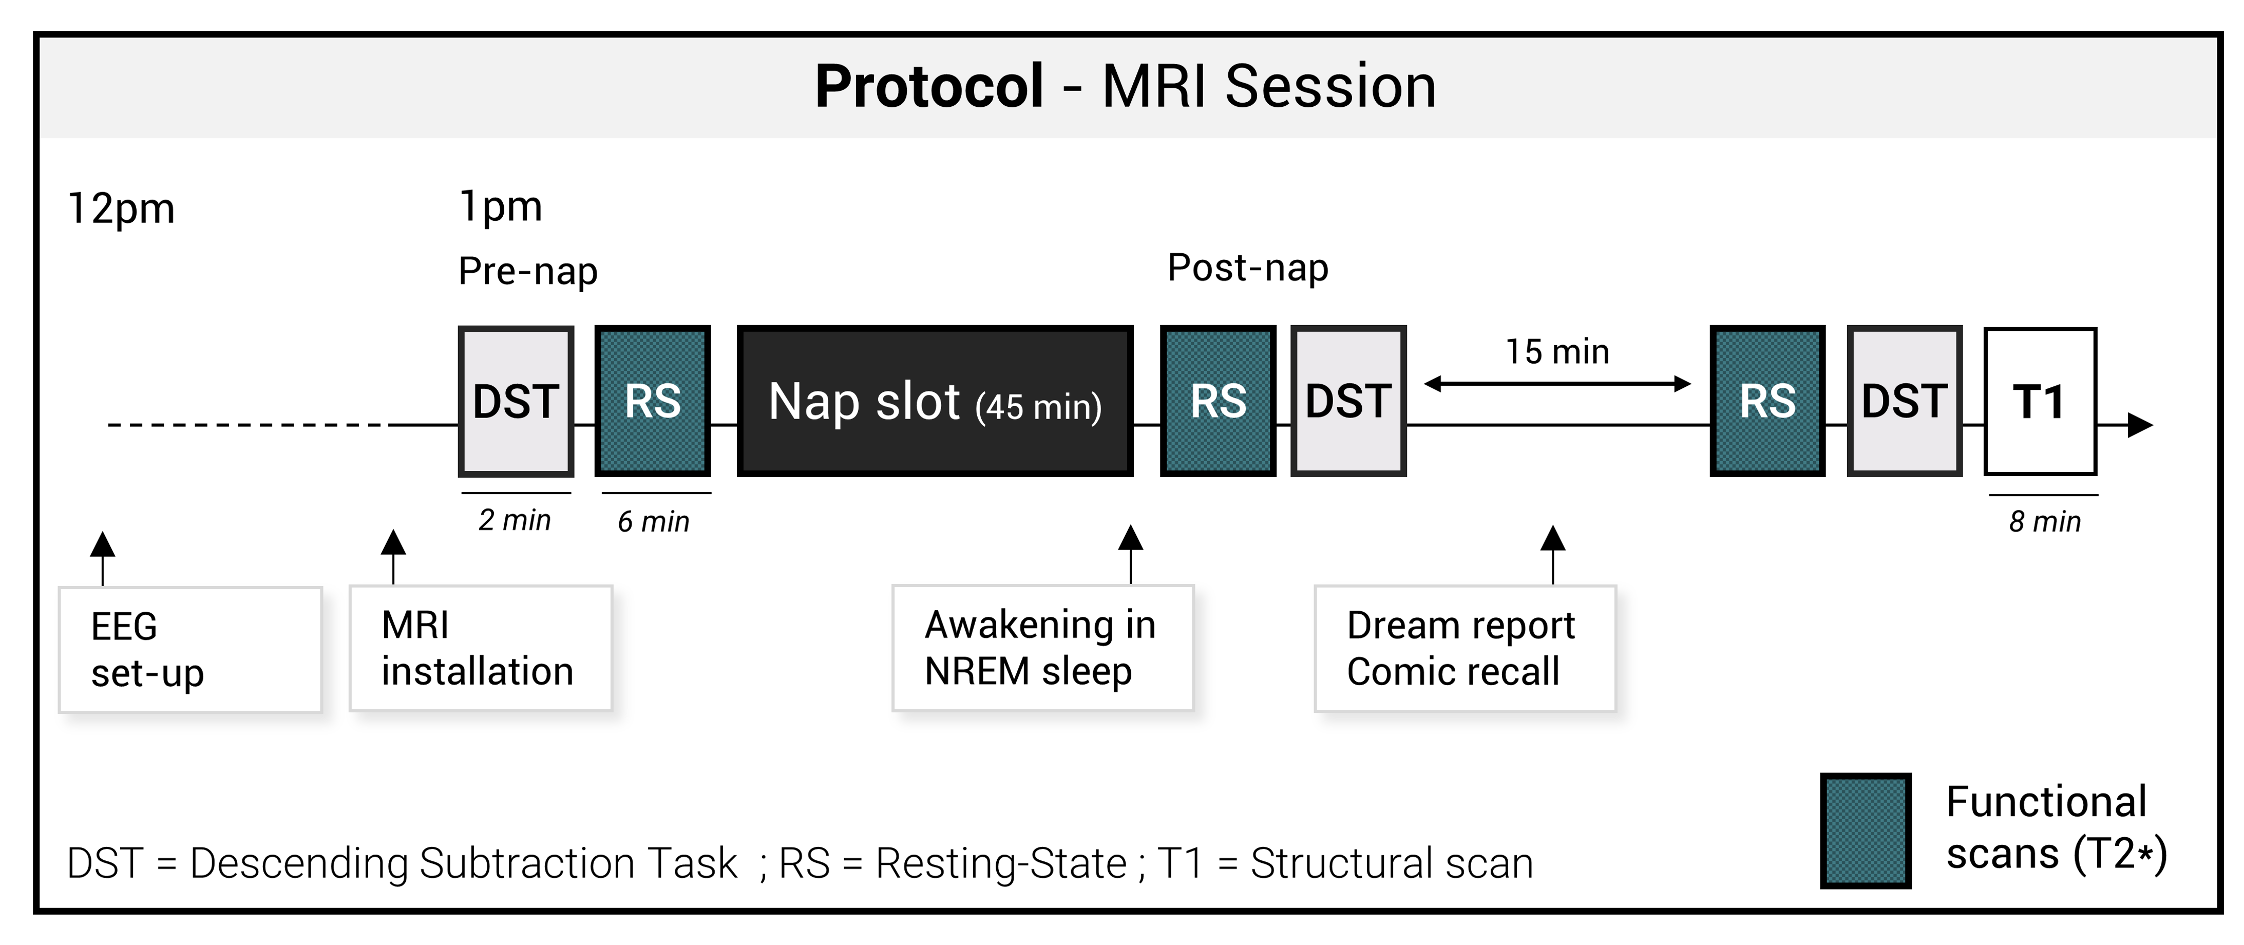
\includegraphics[width=\textwidth]{Fig/Intro/Intro_paradigm_fMRI/Intro_paradigm_fMRI.png}
	\caption[Experimental design of the fMRI study]{\textbf{Experimental design of the sleep inertia fMRI study}. \\
    \emph{Participants}. Participants were selected if they reported and subsequently confirmed during a phone interview having a high or low DRF (DRF superior to 5 dream recalls per week and inferior to 2 dream recalls per month respectively) and having no sleep disturbances. \\
    \emph{Evening and night}. Participants arrived in the sleep unit of the hospital Le Vinatier (Lyon, France) at 8 pm on the evening prior to the experimental day. From 8 pm to 10 pm, they underwent several personality and cognitive tests administered by R.V. They were then instructed to stay awake until 5 am, at which point they were allowed to sleep for 3 hours until 8 am in a bed in the sleep unit. \\
    \emph{Day}. After lunch, participants were conducted to the neuroimaging center (CERMEP). During the first half hour, experimenters installed on the participant’s head a MRI compatible EEG cap. Participants were then installed in the MRI scanner. They read a 5 min comic during the calibration of the eye-tracking camera, and then performed a mental calculation task (descending subtraction task, DST) for 2 minutes. The first resting-state scan was then acquired, with the instructions to remain awake and look at a central fixation cross on the screen. At the end of the scan, participants were informed that they could sleep during the next 45 min. During the nap, the experimenter used the EEG recordings to visually monitor, in real-time, the sleep stages. At the end of the nap slot, participants were awakened, if they were sleeping, by calling their first name and the 2nd resting state scan was acquired. At the end of the scan, the 2nd DST was performed. During the following 10 minutes, subjects were asked about their dream(s) and the comic they had read earlier. Then the 3rd resting state scan and DST were performed (about 25 min after awakening). Finally, an 8-min T1 anatomical scan was acquired.}
	\label{fig:intro:problematics-fmri-paradigm}
\end{figure}

\subsection{Sub-study 2: Brain networks dynamics during sleep inertia}
\label{sec:problematic:inertia:overview}

In addition with comparing the differential brain functional organization of high and low dream recallers during sleep inertia, this study offers the possibility to investigate thoroughly - by pooling the two groups - the brain networks changes across the sleep inertia period. Indeed, while the behavioral aspects of sleep inertia are well documented, only a limited amount of studies investigated its cerebral correlates until now. Our paradigm offers an unique opportunity to study the brain and cognitive alterations during sleep inertia. For instance, one can observe the alterations in functional connectivity that are specific to sleep inertia by contrasting the 5 min post-awakening fMRI scan (RS2, see Fig \ref{fig:intro:problematics-fmri-paradigm}) to the pre-sleep fMRI scan (RS1). Similarly, the evolution of the cerebral alterations of sleep inertia can be evaluated by contrasting the 25 min post-awakening fMRI scan (RS3) to the 5 min post-awakening scan (RS2). In sum, by assessing simultaneously the brain and behavioral changes associated with sleep inertia, our paradigm provides an ideal starting point to study, as wished by \citet{trotti_waking_2016} in her recent review, \q{the which and how functional brain networks are altered in the minutes following awakening}. It should also be noted that participants were partially sleep deprived on the night before, and awakened from a 45 minutes mid-afternoon nap if possible in N3 sleep. Both sleep deprivation and awakening in N3 sleep have been associated with increased sleep inertia \citep{tassi_sleep_2000}. Therefore, in addition with being ecological (short nights compensated by a daytime nap being common in young adults \citep{faraut_napping:_2016}, this paradigm will allow us to study sleep inertia in its most intensified form.

% Using EEG, some studies have found a persistence of slow wave activity in the minutes following awakening, specifically in posterior areas, a phenomenon which has been suggested to represent the electro-physiological signature of sleep inertia \citep{ogilvie_falling_1992, ferrara_electroencephalographic_2006, marzano_recalling_2011, gorgoni_eeg_2015}. Using PET, \citet{balkin_process_2002} reported that the brain areas whose regional cerebral blood flow (rCBF) was increasing between 5 to 20 min post awakening were primarily anterior heteromodal areas (e.g. lateral prefrontal cortices, and anterior insula). They also reported shifts in the relative levels of rCBF between pairs of brain regions (orbitofrontal cortex and ventromedial caudate nucleus, dorsolateral prefrontal cortex and mesencephalic reticular formation) between 5 and 20 min post awakening, leading them to propose that recovery from sleep inertia could hinge on a resumption of normal levels of both rCBF and functional connectivity between brain areas. The latter hypothesis has been tested in two recent resting-state functional magnetic resonance imaging (fMRI) studies which investigated the variations in brain connectivity between pre-sleep wakefulness, nocturnal sleep (without previous sleep deprivation) and post-sleep wakefulness \citep{wu_variations_2012, tsai_local_2014}. Using paired comparisons between pre- and post-sleep wakefulness, they found a decreased connectivity within the sensory-motor network at awakening but no alterations in the default mode network. This altered connectivity within the sensory-motor network is coherent with the poor motor performances observed at awakening but does not explain the impairments observed in other domains (e.g. cognitive tasks such as mental calculation, \citealp{tassi_sleep_2000, trotti_waking_2016}). Yet, some modifications of the default mode network connectivity could be expected at awakening since several neuroimaging studies showed consistent alterations of the default mode network connectivity during sleep, fatigue and/or falling asleep (see \citealp{picchioni_sleep_2013} for a review).

\section{Study 3. DRF, cognitive abilities, and default network functional connectivity}
\label{sec:problematic:dmn-crea}

As we have seen earlier, there is ample evidence that DRF is positively correlated with psychological factors such as creativity or some personality traits (e.g. openness to experience, see section \ref{sec:dream-recall:param:psych} and \ref{sec:dream-recall:param:psych}). On the other hand, recent findings indicate that DRF is also positively associated with distinct neurophysiological traits during both sleep and wakefulness, such as a higher regional cerebral blood flow within core regions of the default mode network. These two observations are remarkably consistent with the emerging view that dreaming and creative-thinking pertain to the same family of spontaneous mental processes, which could be underpinned by a strong recruitment of the default mode network (DMN, \citealp{christoff_mind-wandering_2016}, see section \ref{sec:dream-research:attempts:dmn}) To better delineate the relationship between DRF and the DMN, we re-analyzed the fMRI data of Study 2 to compare, between HR and LR, the functional connectivity of the default mode network, independently of sleep inertia. To this aim, we concatenated the three resting-state scans acquired for each subject, and subsequently compared the global DMN functional connectivity of HR and LR.

Furthermore, we analyzed in this study the numerous cognitive and personality tests that were administered between 8pm and 10pm, on the evening prior to the partial sleep deprivation. Examples of these include the Guildford's Alternate Uses Task \citep{guildford_alternate_1978}, which measures creativity, the Wechsler Memory Scale \citep{wechsler_mem-iii:_2001} to measure memory abilities, and the Big Five Inventory \citep{john_big_1999} which measures an individual on the big five personality dimensions. Regarding the results, we expected that HR would exhibit a higher DMN functional connectivity, specifically between the TPJ and MPFC (see section \ref{sec:dream-recall:param:neuro}), as well as higher scores of creativity and higher scores on certain personality dimensions such as openness to experience. In view of the literature, we did not expect HR to show higher memory abilities than LR.

\FloatBarrier

\section{Study 4. Sleep and dream habits in a sample of French students}
\label{sec:problematic:survey}

Epidemiological investigations in healthy subjects combining questions on both sleep and dreaming are relatively rare. Such measures are yet necessary to establish and keep up to date sleep and dream norms in the general population. Of particular interest is the college population, which is more at risk of suffering from sleep difficulties than the general population \citep{buboltz_sleep_2001, curcio_sleep_2006, forquer_sleep_2008, lund_sleep_2010}.

In order to recruit participants for our above-mentioned fMRI sleep study (section \ref{sec:problematic:inertia}), we have sent an announcement to several mailing lists of students from Lyon University. The announcement comprised a link to an online questionnaire about sleep and dream habits that participants had to fill out. The analysis of the responses provided up-to-date data on sleep and dream habits of a large sample of French college students, pertaining to different academic fields (i.e. humanities, science, medicine). Because our survey included relatively rare questions (e.g. frequency of recurrent and lucid dreams, sleepwalking, sleep-talking, sleep agitation), and thanks to a large sample of students including much more males than in previous studies (i.e. more than one third), we believe that this study will make a significant contribution to the limited number of previous epidemiological studies. Among our main points of interests were (1) to evaluate the sleep patterns of French college students (2) to find whether we could replicate previously reported gender differences in sleep and dream patterns (3) to find whether we could observe some inter academic fields differences.

\section{Study 5. The relationship between waking life and dream content}
\label{sec:problematic:wle}

As we mentioned earlier, there are numerous results showing that waking-life experience (WLE) finds its way into dreams (which led to the so-called continuity hypothesis, \citealp{schredl_continuity_2003}). However, the selection rule and time course of the WLE integration into dreams are still unclear. For instance, few studies have so far investigated the incorporation of WLE from the distant past as well as the incorporation of trivial, mundane, WLE. This is partly due to the classic method used in experimental studies so far, i.e. the content matching paradigm. It requires the participants to rate a posteriori (i.e. at the end of several days of experiment), similarities between a day diary and a dream diary completed for 14 days (e.g. \citealp{schredl_factors_2006, malinowski_evidence_2014}). Such a method has the advantage of controlling for retrospective availability of memories for elements when participants relate dream content to WLEs, but it may have the drawback of missing numerous mundane WLE that are not recorded in the day diary (typically insignificant day-residues), and at the same time overestimating the proportion of emotionally intense WLE. As a consequence, previous studies could not fully assess whether mundane WLEs and/or WLEs from the distant past were incorporated into dreams.

% This is the case for instance regarding the temporal distance between the WLE and its incorporation into dreams on one hand, and the emotional intensity of the WLE on the other hand. Indeed, it is generally admitted that there is a preferential incorporation of recent and emotional WLE into dreams \citep{botman_dream_1990, strauch_dem_2004, grenier_temporal_2005, schredl_factors_2006, malinowski_evidence_2014}. However, some characteristics of dream content do not fit with this modeling of the data. Firstly, some body injuries - be it congenital or acquired - such as amputation, paraplegia and deafness, are less incorporated into dream reports than this model would predict considering how highly emotional and central to the person’s life they are \citep{voss_waking_2011, saurat_walking_2011, bekrater-bodmann_post-amputation_2015}. Secondly, as noticed by \citet{freud_interpretation_1900} more than one century ago, dream content seems to integrate a non-negligible proportion of non-emotional and mundane day residues (i.e. WLEs from the day before the dream).

To address this problem, we designed a study which aimed at investigating in further details the characteristics of the WLEs incorporated into dreams, notably by assessing their remoteness on a life-time scale and by taking mundane WLEs into account. To do so, instead of asking dreamers to keep a day diary, we asked participants to report and characterize the WLEs related to their dreams immediately upon awakening. This strategy presents several advantages regarding previous methods. Firstly, any remembered WLE at any timescale can be considered. This method offers then the possibility of investigating the incorporation of WLEs across the whole life span, which has been rarely attempted until now \citep{grenier_temporal_2005, marquardt_empirical_1996}. Secondly, as the reported memory sources of a dream are dependent on the delay between the dream and the task to report memory sources, the sooner the task after the dream, the more chances we have to identify the true memory sources of the dream \citep{cavallero_dream_1987}. Thirdly, as the connections between elements of waking life and dream content are assessed when the memories of the preceding days are still fresh, this method enables the recall of trivial WLEs from at least the few days before the dream. Using this new approach, we were able to test whether emotional WLEs are still preferentially incorporated into dream reports when trivial WLEs are taken into account and to investigate the emotionality and significance of WLEs incorporated into dreams as a function of their remoteness.

We predicted that this methodology would enable us to observe that a large proportion of the WLEs incorporated into dreams are mundane. Regarding the temporal remoteness of the WLEs incorporated into dreams, we expected to find not only a large contribution of the day before the dream \citep{marquardt_empirical_1996} but also a significant contribution of remote WLEs \citep{verdone_temporal_1965, grenier_temporal_2005, llewellyn_such_2013}. Finally, given previous results showing a tendency for dreams to incorporate preferentially emotional WLEs \citep{schredl_factors_2006, malinowski_evidence_2014}, and the claim that day residues are predominantly mundane \citep{freud_interpretation_1900}, we predicted an interaction between remoteness and emotionality for WLEs incorporated into dreams. Specifically, we expected that day residues would be scored as less important and less emotionally intense than would be more remote WLEs incorporated into dreams.

\section{Study 6. An open-source software for sleep reading and analysis}
\label{sec:problematic:software}

During my PhD thesis, I have been working extensively on polysomnographic sleep recordings, notably to score sleep microstructural events (e.g. arousals, rapid eye movements; see section \ref{sec:problematic:arousals}) and sleep stages (see section \ref{sec:problematic:inertia}). While the detection of sleep microstructural events is usually done with automatic algorithms, the identification of sleep stages is traditionally done visually by an expert. For both visual sleep staging and automatic microstructural analysis, sleep researchers use either commercial or in-house softwares. In many cases, these softwares come with their own data and hypnogram file formats, and this heterogeneity can represent a substantial obstacle for sharing of algorithms and sleep data across laboratories.

% Some of the very few free and open-sources alternatives allowing scoring and to some extent analysis of sleep data are \fnurl{Phypno}{https://pypi.python.org/pypi/phypno} and \fnurl{SpiSOP}{http://www.spisop.org/}, yet they do not include graphical integration of automatic detection and are largely based on command-line options, which are hardly accessible for users with little or no programming knowledge.

% Traditionally, the scoring of sleep micro- and macro-structure is done visually and requires therefore a considerable investment of time and effort, in addition with being subject to both inter and intra-rater variability. Sleep scoring can also be done using automatic methods which have the advantage of being fast, reproducible and with generally good agreement with visual scoring \citep{berthomier_automatic_2007, lajnef_learning_2015}. Yet automatic scoring is far from being widespread and most sleep laboratories still rely on visual scoring, using either commercial softwares or in-house packages. In many cases, these softwares come with their own data and hypnogram file formats, and this heterogeneity can represent a substantial obstacle for sharing of algorithms and sleep data across laboratories or clinics. Some of the very few existing and up-to-date open sources alternatives allowing reading and scoring of sleep data are \fnurl{Phypno}{https://pypi.python.org/pypi/phypno} and \fnurl{SpiSOP}{http://www.spisop.org/}, yet they do not include graphical integration of automatic detection and are largely based on command-line options, which are hardly accessible for users with little or no programming knowledge.

In view of this, I developed, during my PhD thesis, a free and open-source software capable of reading numerous file formats, and integrating several signal processing tools and automatic detection of sleep microstructure. At first intended for my personal use, it soon extended into a fully developed and comprehensive software, thanks to a collaboration with my fellow PhD student \fnurl{Etienne Combrisson}{https://etiennecmb.github.io/}. This software was integrated into a broader neuroscientific suite named \fnurl{Visbrain}{http://visbrain.org/}, and the specific sleep module was named \textit{SLEEP}. The primary aim of \textit{SLEEP} is to provide a fast and intuitive graphical user interface (GUI) to visualize and score polysomnographic sleep recordings. In order to be widely disseminated, the software must support a large range of data file formats, both proprietary (e.g. BrainVision) and public (e.g. European Data Format). It should also be able to handle the great heterogeneity in hypnogram formats (e.g. sampling rate of the hypnogram, values assigned to each sleep stage). Finally, to provide a significant scoring aid, the software should include several automatic detection algorithms (e.g. spindles, K-complexes, slow-waves) and several signal processing tools (e.g. filtering, referencing). Altogether, we believe that this software could represent a major methodological development in the field of sleep research.

\section{Summary}
\label{sec:problematic:summary}

\begin{figure}[htb]
	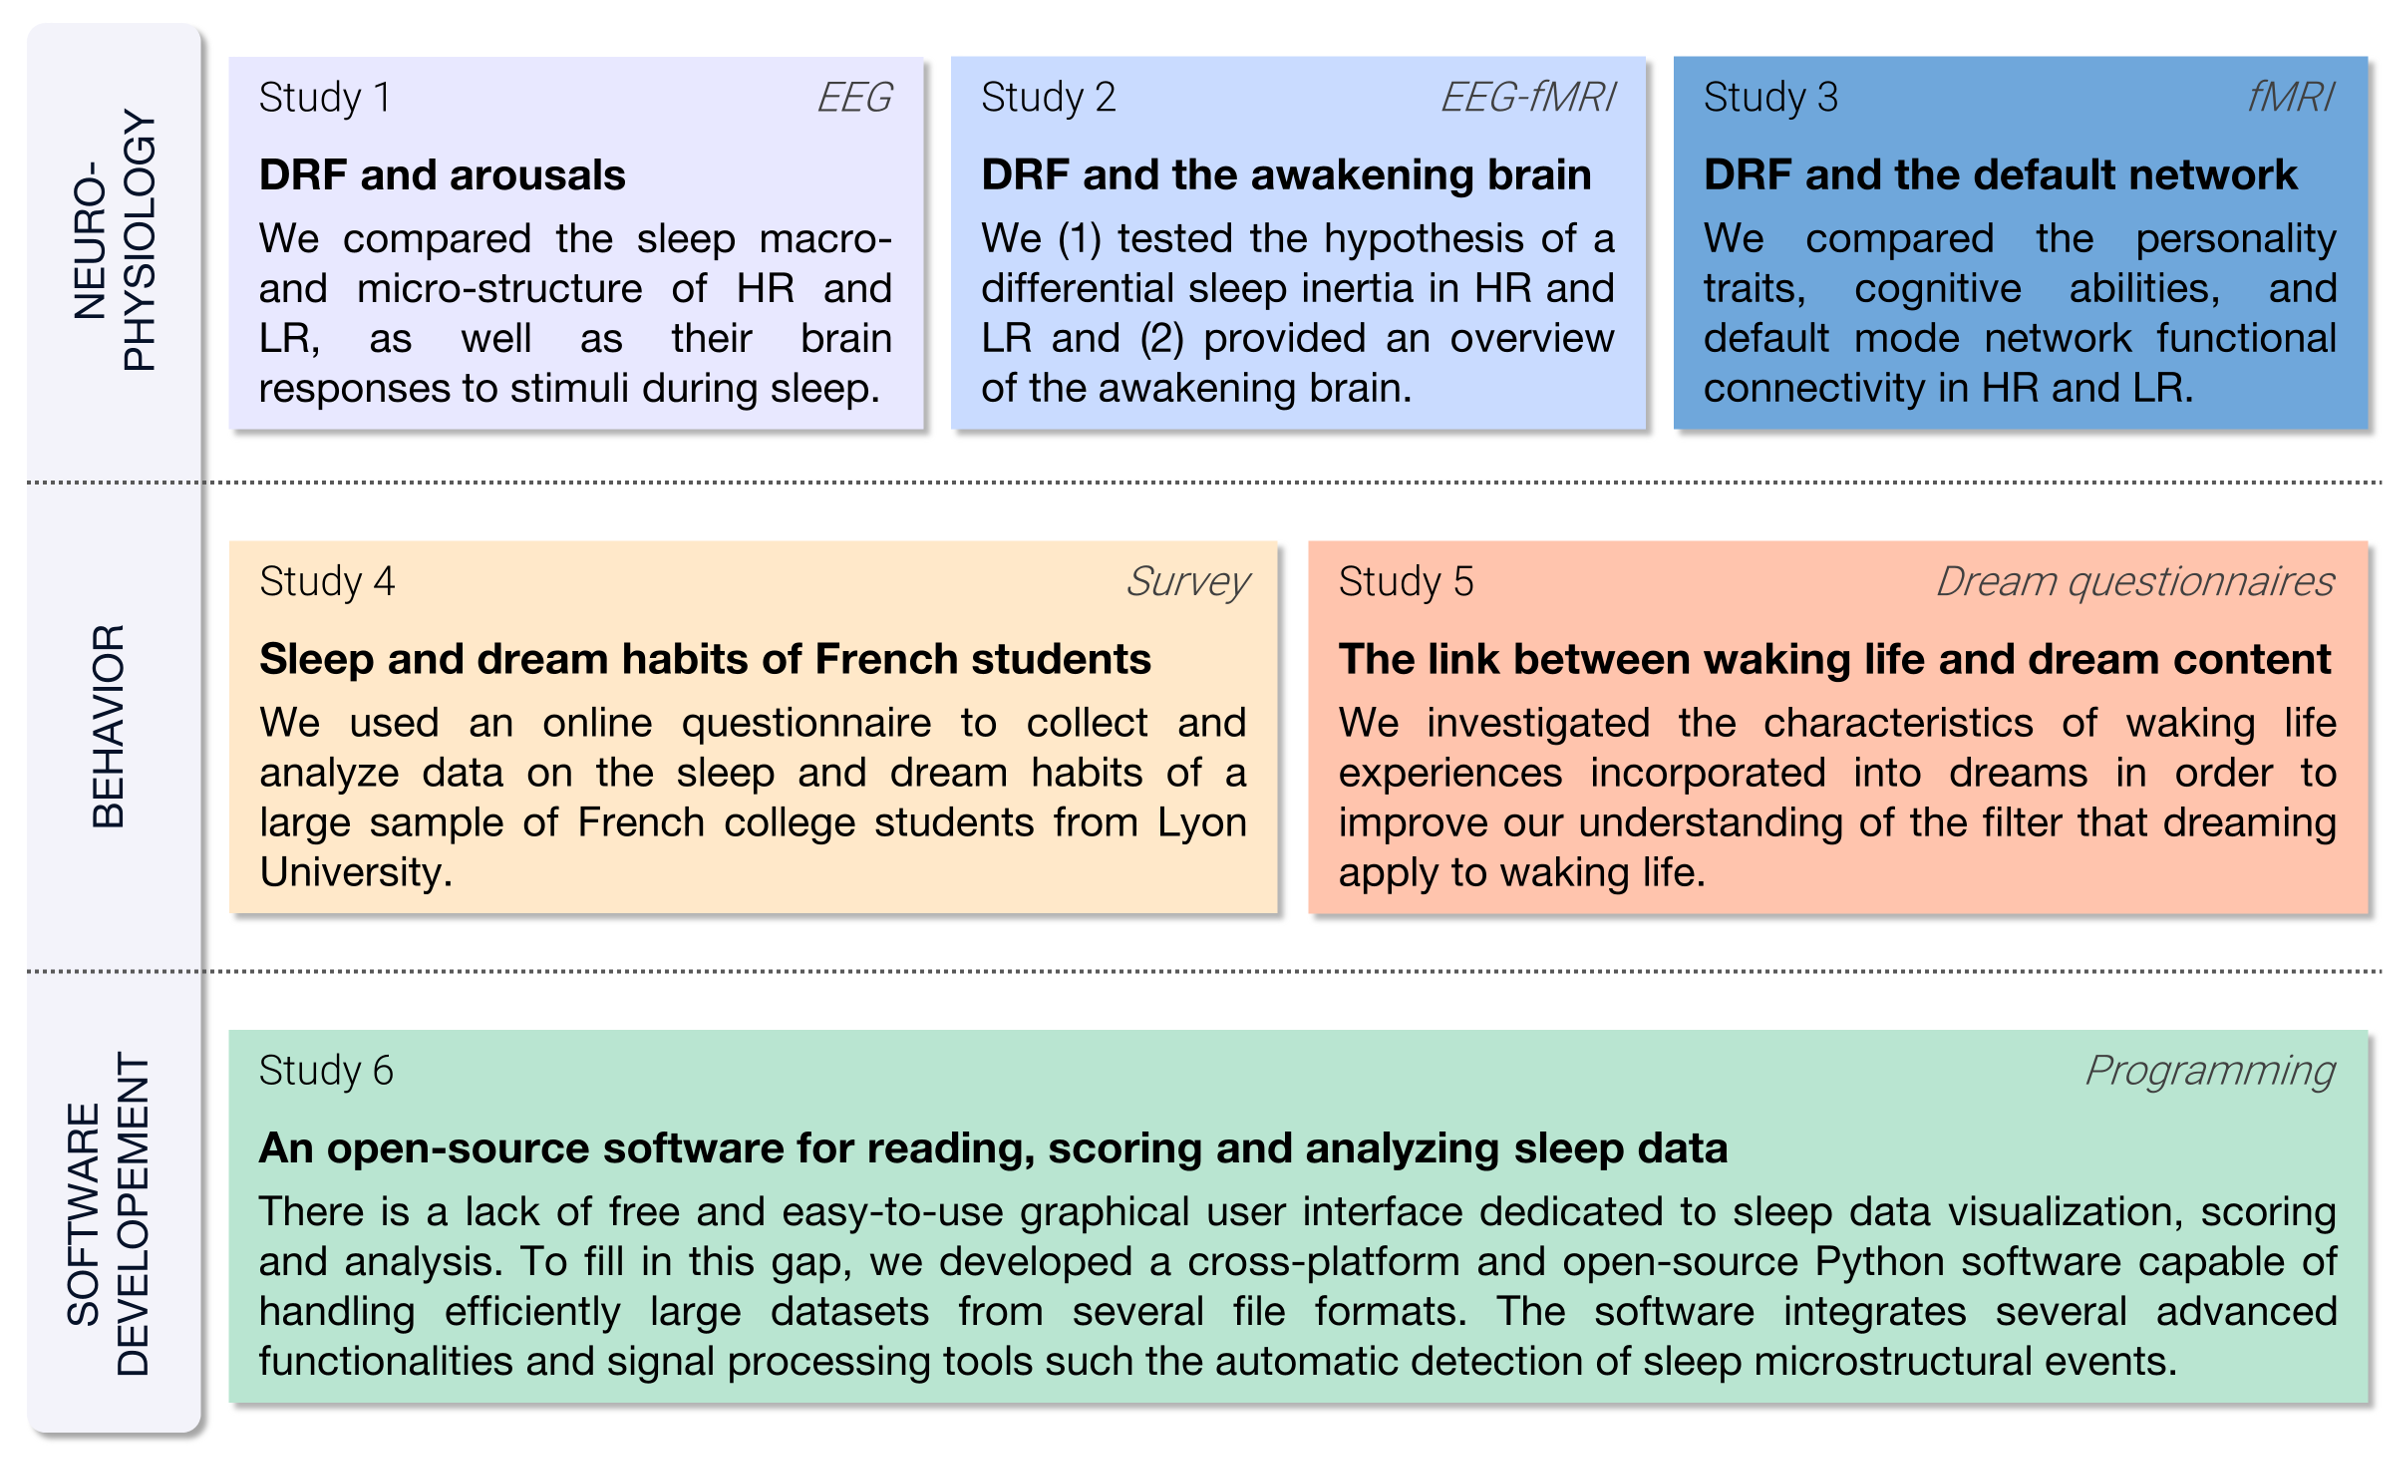
\includegraphics[width=\textwidth]{Fig/Intro/Intro_Problematics/Intro_Problematics.png}
	\caption[Summary of the studies conducted during my PhD thesis]{\textbf{Summary of the studies conducted during my PhD thesis}. In Studies 1, 2 and 3, we investigated the neurophysiological correlates of dream recall frequency (DRF), by comparing the sleep parameters, cognitive abilities and brain functional connectivity of high and low dream recallers (HR and LR respectively). Second, we used behavioral methods to collect data on the sleep and dream habits of college students (Study 4), as well as the relationship between waking life and dream content (Study 5). Finally, Study 6 relates to the ongoing development of an open-source software dedicated to sleep data.}
	\label{fig:intro:problematics-summary}
\end{figure}


\part{METHODS}
\cleardoublepage

\chapter{EEG and event-related potentials}
\label{sec:eeg}

\section{Electro-encephalography (EEG)}
\label{sec:eeg:eeg}

The first recording of the electric field of the human brain was made by the German psychiatrist Hans Berger in 1924. He named this recording electroencephalogram (EEG; \citealp{berger_uber_1929}). Since then, EEG and event-related potentials (ERP; see next section) have become one of the most prominent technique in research (e.g. neuroscience, psychology) and medical settings (e.g. epilepsy, sleep disorders). EEG records voltage fluctuations resulting from ionic current within large assemblies of neurons in the brain. The brain electrical activity is measured with electrodes that are placed either along the scalp or, in rarer circumstances, directly on the exposed surface of the brain (electro-corticography or intra-cranial EEG). Through the current thesis, we will focus solely on the former and non-invasive, scalp EEG method, which is also one of the three essential electrophysiological measurements of polysomnography, along with EOG and EMG (see section \ref{sec:dream-research:sleep:stages}).

\subsection{International 10-20 system}
\label{sec:eeg:eeg:10-20}

EEG is generally recorded from multiple electrodes distributed across the scalp. To allow reproducibility both within and between individuals, the placement of these electrodes is defined in the internationally standardized 10-20 system, which relies on the relationship between the location of an electrode and the underlying area of cerebral cortex (Figure \ref{fig:methods:10-20}). Electrode location are determined using two standard anatomical landmarks, the nasion and inion, respectively located between the eyes and at the back of the skull. From these points, the skull perimeters are measured in the transverse and median planes and electrode locations are determined by dividing these perimeters into 10\% and 20\% distance intervals. Electrodes names refer to their locations on the cerebral cortex. Thus, the first letter refers to the brain lobe on which they are located (F = frontal, C = central, P = parietal, O = occipital), while the number corresponds to the hemispheres (3 = left, 4 = right). For example, F3 is located on the left hemisphere of the frontal lobe, while P4 lies on the right hemisphere of the parietal lobe.

\begin{figure}[htb]
	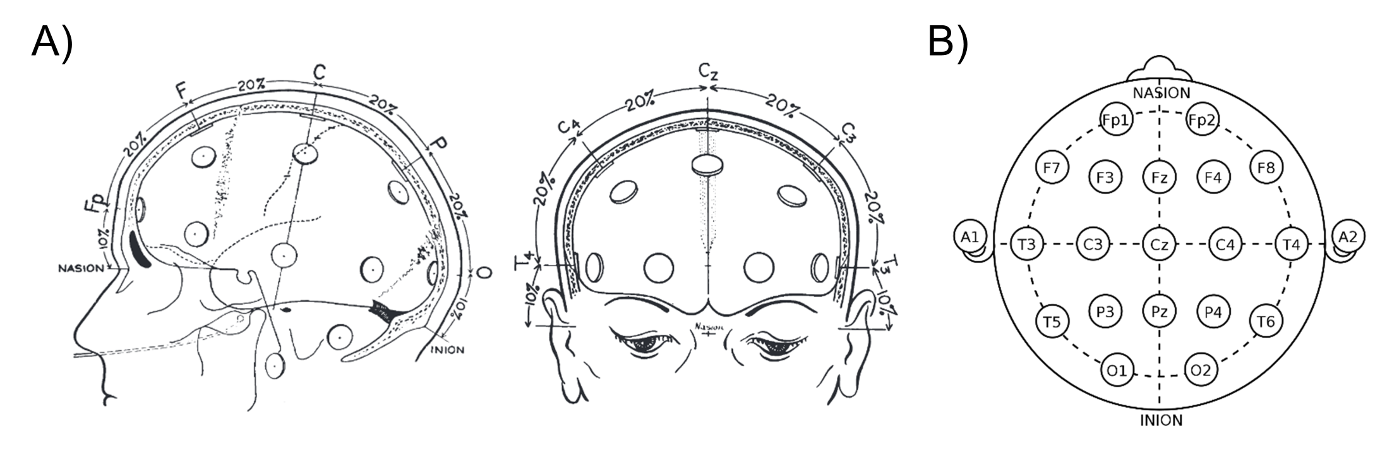
\includegraphics[width=\textwidth]{Fig/Methods/EEG_10-20/EEG_10-20.png}
	\caption[Electrode locations of International 10-20 system for EEG recording]{Electrode locations of International 10-20 system for EEG recording. (A) Lateral and frontal views of the skull showing the methods of measurement for electrode placement (adapted from \citealp{klem_ten-twenty_1999}). (B) Single plane projection of the head showing all standard positions and names of electrodes according to the 10-20 system. }
	\label{fig:methods:10-20}
\end{figure}

\subsection{Amplification, filtering and montage}
\label{sec:eeg:eeg:ampli}

The brain electrical activity is quite small (usually under 100 µV). For that reason, the EEG signal recorded on the scalp must be first amplified by several thousand times. In modern, digital EEG, the signal from each channel is then turned into a series of discrete digital values, with a sampling frequency generally comprised between 200 to 5000 Hz. The signal is then filtered and displayed on a computer screen using dedicated softwares such as Elan \citep{aguera_elan:_2011} or EEGLAB \citep{delorme_eeglab:_2004}. Typical filters include high-pass (<0.1 Hz), low-pass (35-70 Hz), and notch (50 or 60 Hz) to remove very slow artefacts, high-frequency artefacts (such as electromyographic activity) and electrical noise, respectively.
Since the EEG is measured as the voltage (i.e. potential for electrical charges to move between two locations) between two electrodes, the display of EEG may be set up in several ways, referred to as montage. In the standard, referential montage, a single reference electrode, located at a site thought to be electrically neutral, such as the earlobe or the mastoid, is typically used for all the active scalp electrodes. By contrast, in the average reference montage, the averaged signal across all electrodes is used as the common reference for each channel.

\subsection{Neural oscillations}
\label{sec:eeg:eeg:neural}

The spontaneous brain electrical activity is characterized by rhythmic oscillations, which are sometimes referred to as neural oscillations or, more popularly, as \q{brain waves}. These oscillations are generated by the summation of synchronous activity of thousands or millions or neurons (mainly cortical pyramidal neurons). They have characteristic frequency ranges, spatial distributions and are associated with different states of brain functioning (e.g. waking and the various sleep stages; see Figure \ref{fig:methods:neural}).

\begin{figure}[htb]
	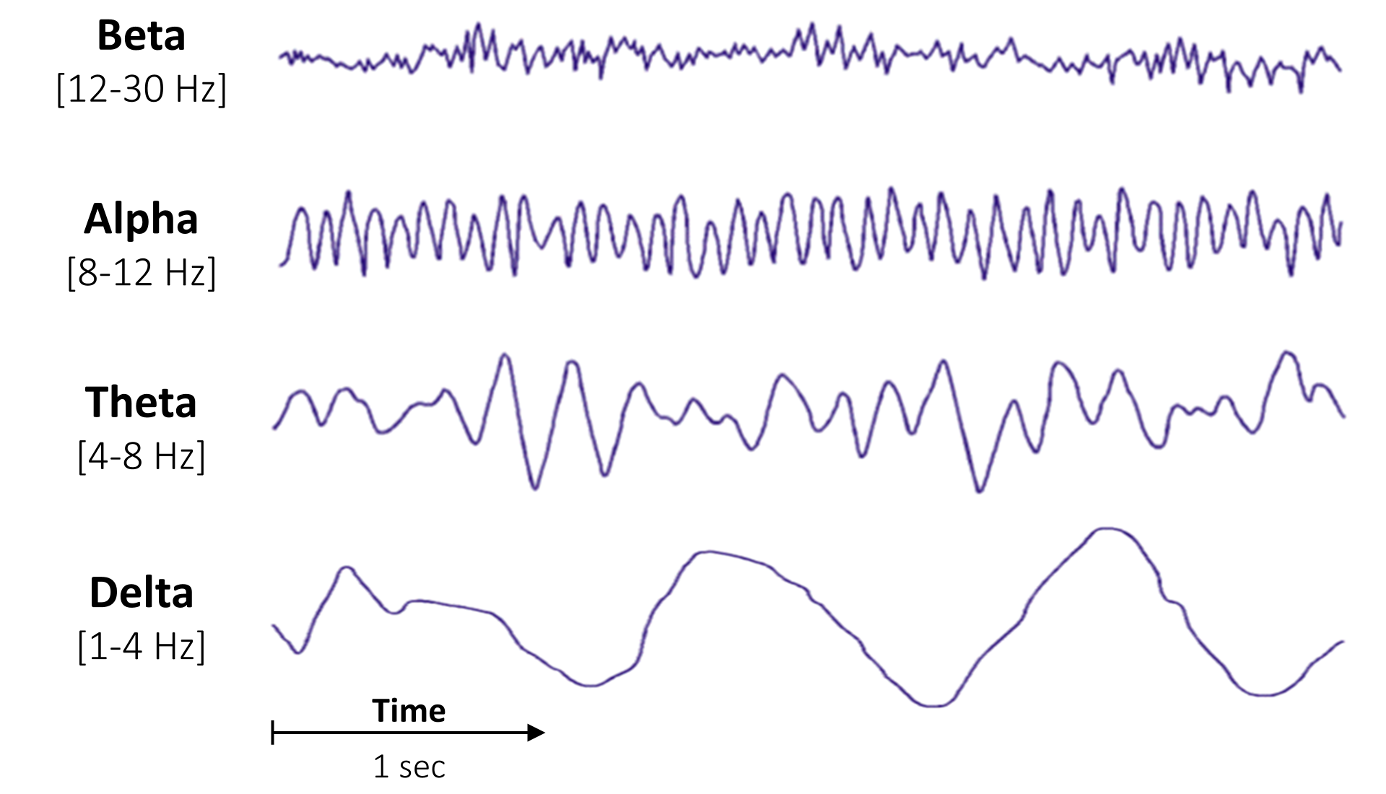
\includegraphics[width=\textwidth]{Fig/Methods/EEG_BrainWaves/EEG_Brain_Waves.png}
	\caption[Brain rhythms]{Brain rhythms. Beta waves are prominent over occipital and parietal areas during normal waking wakefulness. Alpha waves are prominent in occipital regions during eyes-closed wakefulness. Theta waves are detectable during N2 sleep and REM sleep. Delta waves are visible during N3 sleep (also called slow-wave sleep or deep sleep) and have a large amplitude (>75 µV) due to a high level of neural synchronization.}
	\label{fig:methods:neural}
\end{figure}

\section{Event-related potentials (ERP)}
\label{sec:eeg:erp}

\subsection{Definition and methods}
\label{sec:eeg:erp:def}

Event-related potentials (ERPs) are \q{electrical potentials generated by the brain that are related to specific internal or external events such as stimuli, responses or decisions} \citep{luck_introduction_2014}. A single ERP, usually recorded by means of scalp EEG, has an amplitude ranging from 0.5 to 15 µV, and is therefore much lower than the spontaneous background EEG (100 µV). As a consequence, a single ERP is not visible to the naked eye in the EEG signal. In order to disentangle and reveal the specific relevant ERP from the irrelevant background EEG, ERP technique relies on the mathematical principle of summation. It consists of averaging hundreds of time-locked repetitions of the same experimental condition in order to attenuate activities that are unrelated to the specific internal or external event.
The resulting waveform contains a series of positive and negative peaks (components) that are thought to reflect activity (i.e. postsynaptic potentials) in underlying generators within the brain. These components are usually referred to with acronyms (e.g. contingent negative variation, CNV) or by a letter indicating polarity (N = negative, P = positive), followed by a number indicating the latency in milliseconds from stimulus onset (e.g. N100 is a negative peak arising approximatively 100 ms after stimulus). Early components, which arise approximatively less than 80 ms after the stimulus, are thought to reflect sensory processes and are therefore intrinsically linked to the physical characteristics of the stimulus. By contrast, late components (>100ms) are thought to reflect more cognitive processes such as attention, memory and response preparation. They differ from the former in the sense that they are not systematically elicited but rather require the participant to be involved in some stimulus-related task (e.g. a detection task). While some potentials are easily obtain by repetition of stimuli (e.g. the N100 potential, elicited by perception of auditory stimuli), others potentials are elicited by more complex paradigm. One of the most famous is probably the oddball-paradigm, in which low-probability target (or \textit{deviant}) items are mixed with high-probability non-target (or \textit{standard}) items. Target items elicit a late positive component, the P300, though to reflect brain processes involved in stimulus evaluation or categorization.

\begin{figure}[htb]
	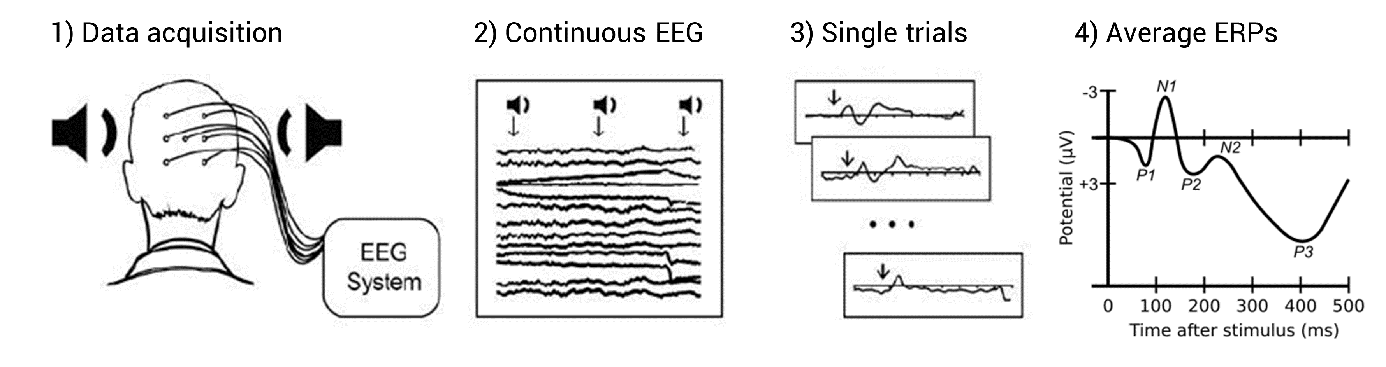
\includegraphics[width=\textwidth]{Fig/Methods/ERP/ERP.png}
	\caption[Schematic representation of ERP acquisition]{Schematic representation of ERP acquisition. (1) Scalp electrodes record electrical brain activity while auditory stimuli are presented repeatedly through headphones or speakers. (2) Stimulus onset/offset markers are recorded along with the continuous EEG signal. (3) Individual segments locked to stimulus onset are extracted from the continuous EEG and include a brief pre-stimulus baseline in addition to post-stimulus period of interest. (4) Averaged ERP waveform showing several components (including the N100 and P300) reflecting time- and phase-locked neural activity associated with stimulus processing. Note that the ERP is plotted with negative voltages upward, a common, but not universal, practice in ERP research. Adapted from \citet{key_human_2016}}
	\label{fig:methods:erp}
\end{figure}

\subsection{The use of ERP in sleep research}
\label{sec:eeg:erp:erp}

ERP is a method of choice for the investigation of the normal and pathological human sleep \citep{bastuji_evoked_1999, colrain_use_2007}. One reason for this is that it allows to study objectively information processing during sleep, limited otherwise by the lack of the ability of subjects to make verbal or motor responses to stimuli. It provides a powerful, objective and non-invasive means to study for example the extent of sensory integration during sleep, or the neurological abnormalities related to sleep disorders, or sleep inertia upon waking \citep{bastuji_event-related_2003}.
ERP studies greatly improved our understanding of sleep, from the classical view that sleep is a “little death” (illustrated by the fraternal link between Hypnos, God of Sleep, and Thanatos, God of Death, in the Greek mythology; see \citealp{mazza_asleep_2014}), to the emerging idea that sleep is a dynamic process in which complex cognitive processing occur \citep{andrillon_sleeping_2016}. For example, a P300 component has been observed during REM sleep in response to target stimuli presented within an oddball paradigm \citep{bastuji_brain_1995}. Similarly, there is a persistence of the brain’s ability to detect semantic incongruity during REM sleep  (N400; \citealp{perrin_detection_2002}).
It should however be noted that considerable differences exist between waking, NREM and REM sleep ERP components \citep{bastuji_evoked_1999, colrain_use_2007}. Specifically, while early sensory components (i.e. peripheral and brainstem responses) remain unaffected by the sleep cycle, early cortical responses are drastically modified, in part because the thalamus stops relaying sensory information to the brain. Finally, late cortical responses displays profound changes during NREM sleep, which revert in REM sleep.

\cleardoublepage

\chapter{fMRI and functional connectivity }
\label{sec:fmri}

\section{Structural and functional magnetic resonance imaging}
\label{sec:fmri:fmri}

\subsection{Magnetic resonance imaging (MRI)}
\label{sec:fmri:fmri:mri}

Magnetic resonance imaging (MRI) is probably the \q{most important imaging advance since the introduction of X-rays by Conrad Röntgen in 1895} \citep{logothetis_what_2008}. It is undoubtedly true that the emergence of MRI has indeed marked the beginning of a new era in diagnostic medicine and basic research. MRI is based upon nuclear magnetic resonance, the physical phenomenon by which nuclei placed in an external magnetic field absorb and re-emit radio-frequency energy. MRI is the technique of choice for imaging brain structure, in part because magnetic properties of hydrogen nuclei vary with the biological tissue in which they are. Consequently, the rate of spin relaxation (i.e. how quickly spins \emph{forget} the direction in which they are oriented) is not the same between gray and white matter, which thus makes it possible to construct detailed images of the brain at any location and orientation with sub-millimeter resolution.

\subsection{Functional MRI (fMRI)}
\label{sec:fmri:fmri:fmri}

Functional MRI (fMRI), built on the earlier concept of MRI, is a technique for measuring hemodynamic changes (i.e. blood flow dynamic) in the brain due to changing neural activity. Compared to structural MRI, the brain is scanned at lower spatial resolution (2-3 mm) but at a higher temporal resolution (typically a few seconds). Specifically, fMRI relies on the fact that hemoglobin in blood slightly distorts the magnetic resonance properties of hydrogen nuclei in its vicinity, and the amount of magnetic distortion changes depending on whether the hemoglobin has oxygen bound to it. For example, when neurons of a specific brain area become active, local blood flow to this region increase, and oxygen-rich (oxygenated) blood displaces oxygen-depleted (deoxygenated) blood around 2 seconds later (a phenomenon known as the hemodynamic response). These changes in the concentration of oxygen and blood flow lead to localized blood oxygenation level-dependent (BOLD) changes in the magnetic resonance signal. It is generally accepted that, in most brain regions, the fMRI signal is coupled to the level of excitatory and inhibitory synaptic transmission and therefore reflect the level of information processing \citep{logothetis_what_2008}.

\subsection{Task-based and resting-state paradigms}
\label{sec:fmri:fmri:paradigm}

Traditionally, fMRI has been used to produce maps of task-dependent brain function using block or event-related designs, which are based on the subtraction paradigm. In such designs, one infers the level of activation of certain brain areas by looking at the relative changes from baseline (resting or control condition) in the BOLD signal during the performance of a task or in response to a stimulus. During these designs, participants are instructed to perform specific tasks, which are generally designed to target a single brain function such as vision, attention, memory, emotion recognition and so on. These paradigms have allowed brain science to take giant strides, in particular on the issue of linking brain areas with specific functions (which was in the past only possible by studying cerebral lesions).

More recently, there has been a growing interest in the application of resting-state fMRI (RS-fMRI). Indeed, soon after the development of fMRI, some researchers observed that the resting brain was not silent but contained information about its functional organization \citep{biswal_functional_1995}. Specifically, they reported that, during rest, time courses of low frequency fluctuations (<0.1 Hz) in somatomotor brain areas, showed a high degree of temporal correlation. They argued that this correlation, which may arise from fluctuations in blood oxygenation or flow, is a manifestation of functional connectivity of the brain. Although at the time Biswal’s seminal observation was mostly disregarded, it laid the basis for the now widely-used resting-state fMRI paradigm, which measures how different regions of the brain communicate while participants are not performing any active task. Although both resting-state and task-related designs measures BOLD signal, there are several major differences between the two, which are reported in Table \ref{tab:method:fMRI-paradigm}.

\begin{table}[htb]
    \centering
    \caption[Key differences between task-based fMRI and resting-state fMRI]{\textbf{Key differences between task-based fMRI and resting-state fMRI}. Modified from \citet{smitha_resting_2017}}
    \label{tab:method:fMRI-paradigm}
    \begin{tabularx}{\textwidth}{lXX}
    \toprule
                          & Task-based fMRI                                                                                                 & Resting-state fMRI                                                                   \\ \midrule
    Design                & Analyses of the relative changes from baseline in the BOLD signal during a task or in response to a stimulus    & Analyses of the spontaneous BOLD signal in the absence of any explicit task or input \\
    Energy consumption    & Task-specific increase in neuronal metabolism are less than 5\%                                                 & 60–80\% of brain’s energy is consumed during resting state                           \\
    Brain areas           & The focus is only on a very small fraction of the brain’s overall activity                                      & The focus is on large-scale brain networks                                           \\
    Signal-to-noise ratio & Low since 80\% of the BOLD modulation is discarded as noise                                                     & Good since it takes the overall spontaneous low frequency fluctuations               \\
    Patient cooperation   & Patient cooperation is essential                                                                                & Pediatric, psychiatric and comatose patients can do it                               \\
    Duration              & Requires a large number of repetitions                                                                          & Usually 6 to 10 minutes                                                              \\ \bottomrule
    \end{tabularx}%
\end{table}

\section{Functional connectivity}
\label{sec:fmri:fc}

\subsection{Overview}
\label{sec:fmri:fc:overview}

Functional connectivity can be defined as \q{the temporal dependence of neuronal activity patterns of anatomically separated brain regions} \citep{van_den_heuvel_exploring_2010}. It can be measured as long-range synchronization of the EEG, magneto-encephalography (MEG), or other dynamic brain signals. Applied to fMRI, functional connectivity reflects the temporal correlation of low frequency (<1 Hz) BOLD spontaneous fluctuations in spatially distinct brain regions (Fig \ref{fig:methods:fcmri}). Although the true neuronal basis of these slow BOLD fluctuations is not yet fully understood, there is converging evidence that they result from co-activation in the underlying spontaneous neuronal activation patterns. As a consequence, they are thought to reflect functional communication between brain areas. There are also several evidences that spontaneous BOLD fluctuations are partly constrained by anatomic connectivity \citep{van_dijk_intrinsic_2010}.

In more practical terms, these intrinsic BOLD fluctuations are nearly always measured at rest in order to minimize task-evoked effect. Resting-state fMRI has also the advantage of being quite simple to implement. For that reason, functional connectivity resting-state MRI has become the technique of choice to study the intrinsic functional organization of the brain in healthy individuals across a variety of vigilance states (such as sleep) but also in patients (e.g. comatose and psychiatric patients).

\begin{figure}[htb]
	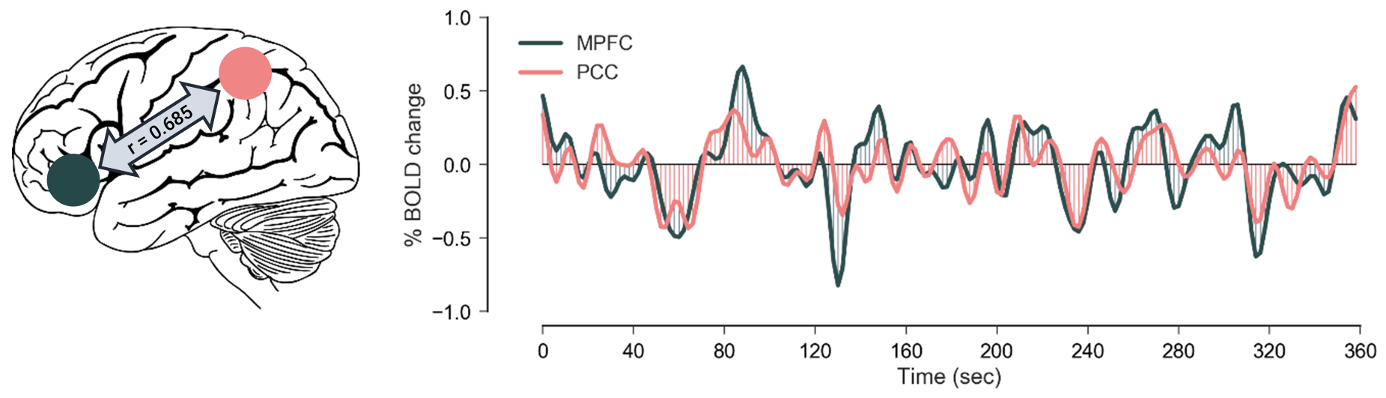
\includegraphics[width=\textwidth]{Fig/Methods/fMRI_temporal_correlation/fMRI_temporal_correlation.png}
	\caption[The basic strategy of functional connectivity MRI]{\textbf{The basic strategy of functional connectivity MRI}. The basis of functional connectivity is that spontaneous BOLD fluctuations measured at rest are correlated between spatially distinct brain regions. In this example, spontaneous BOLD fluctuations in the medial prefrontal cortex (MPFC) and posterior cingulate cortex (PCC) are correlated (Pearson r = 0.685). These data come from a 6-min resting state scan acquired in a single individual on a 3-tesla MRI scanner.}
	\label{fig:methods:fcmri}
\end{figure}

\subsection{Large-scale brain networks}
\label{sec:fmri:fc:network}

A decade of resting-state fMRI research has revealed that the human brain is organized into several large-scale functionally-correlated brain networks, which are consistently found in healthy subjects, different stages of consciousness and across species \citep{fox_spontaneous_2007, yeo_organization_2011}. Because they are preferentially identified during resting-state fMRI, these networks are often referred to as resting-state networks. They are comprised of different brain regions that each have their own task and function, but which are continuously exchanging information with each other. Remarkably, they closely match the topographies of functional responses obtained by task-related fMRI using typical sensory, motor, and cognitive paradigms.
The main functional networks of the human brain are depicted in Fig \ref{fig:methods:networks}. The visual and somatomotor networks include regions of the primary and secondary visual and sensory-motor cortex respectively. These two sensory networks are characterized by a clear coupling between anatomic and functional connectivity \citep{van_dijk_intrinsic_2010}. Next, come the so-called task-positive networks, namely the frontoparietal (FP; sometimes referred to as executive, or control) network, the dorsal attention network (DAN), and the salience network. They are all involved in attentional processes. For instance, the DAN is thought to support selective attention to sensory features of the environment, while the salience network is involved in monitoring the salience of external inputs and internal brain events. There is emerging evidence that the FP network, originally thought to be involved in the selection of sensory contents by attention, may also orchestrate the interactions between other networks \citep{christoff_mind-wandering_2016}.

\begin{figure}[htb]
    \centering
	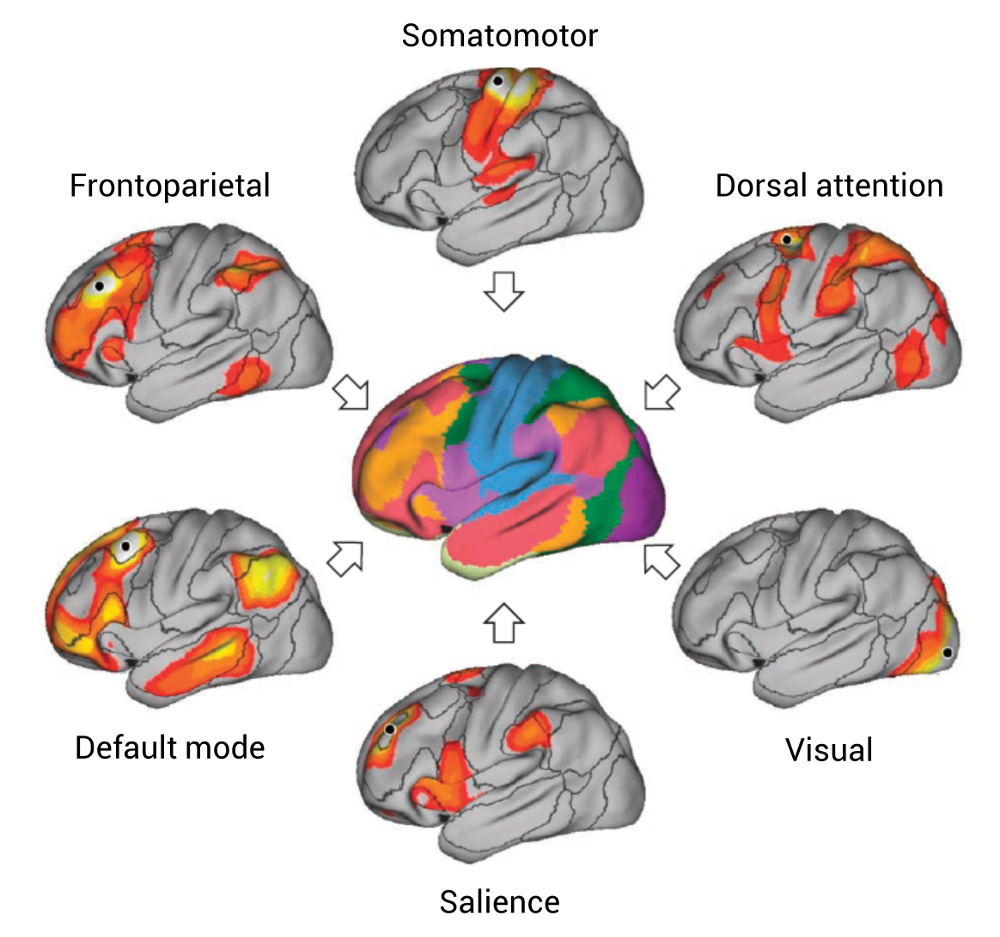
\includegraphics[width=0.9\textwidth]{Fig/Methods/fMRI_Networks/fMRI_Networks.png}
	\caption[Large-scale brain networks]{\textbf{Large-scale brain networks identified with resting-state functional connectivity fMRI}. Outer maps show the functional connectivity maps for a single seed region (black circle) placed in a different cortical region, obtained using resting-state fMRI data in 1000 subjects. Center map shows a composite estimate of the networks using an analytical approach to parcellate cortical regions into their most dominant network. Originally published in \citet{buckner_opportunities_2013}}
	\label{fig:methods:networks}
\end{figure}

Finally, the last and perhaps most investigated brain network is the default mode network (DMN, sometimes referred to as task-negative network), which was originally identified as a set of brain areas consistently deactivated across a range of externally oriented tasks \citep{raichle_default_2001}. It has been linked to internal mental processes, such as introspection, mind-wandering but also episodic memory retrieval and autobiographical future thinking. The DMN includes several subsystems which are supposedly involved in different functional roles  (Fig \ref{fig:methods:dmn}; \citealp{andrews-hanna_functional-anatomic_2010}). The DMN is probably one of the more robust brain network, and it has been identified across several vigilance states, including NREM and REM sleep \citep{horovitz_decoupling_2009, larson-prior_cortical_2009, larson-prior_modulation_2011, wu_variations_2012}. Recently, some authors have postulated that the DMN might be involved in the production and/or encoding of dreams (see section \ref{sec:dream-research:attempts:dmn}).

\begin{figure}[htb]
    \centering
	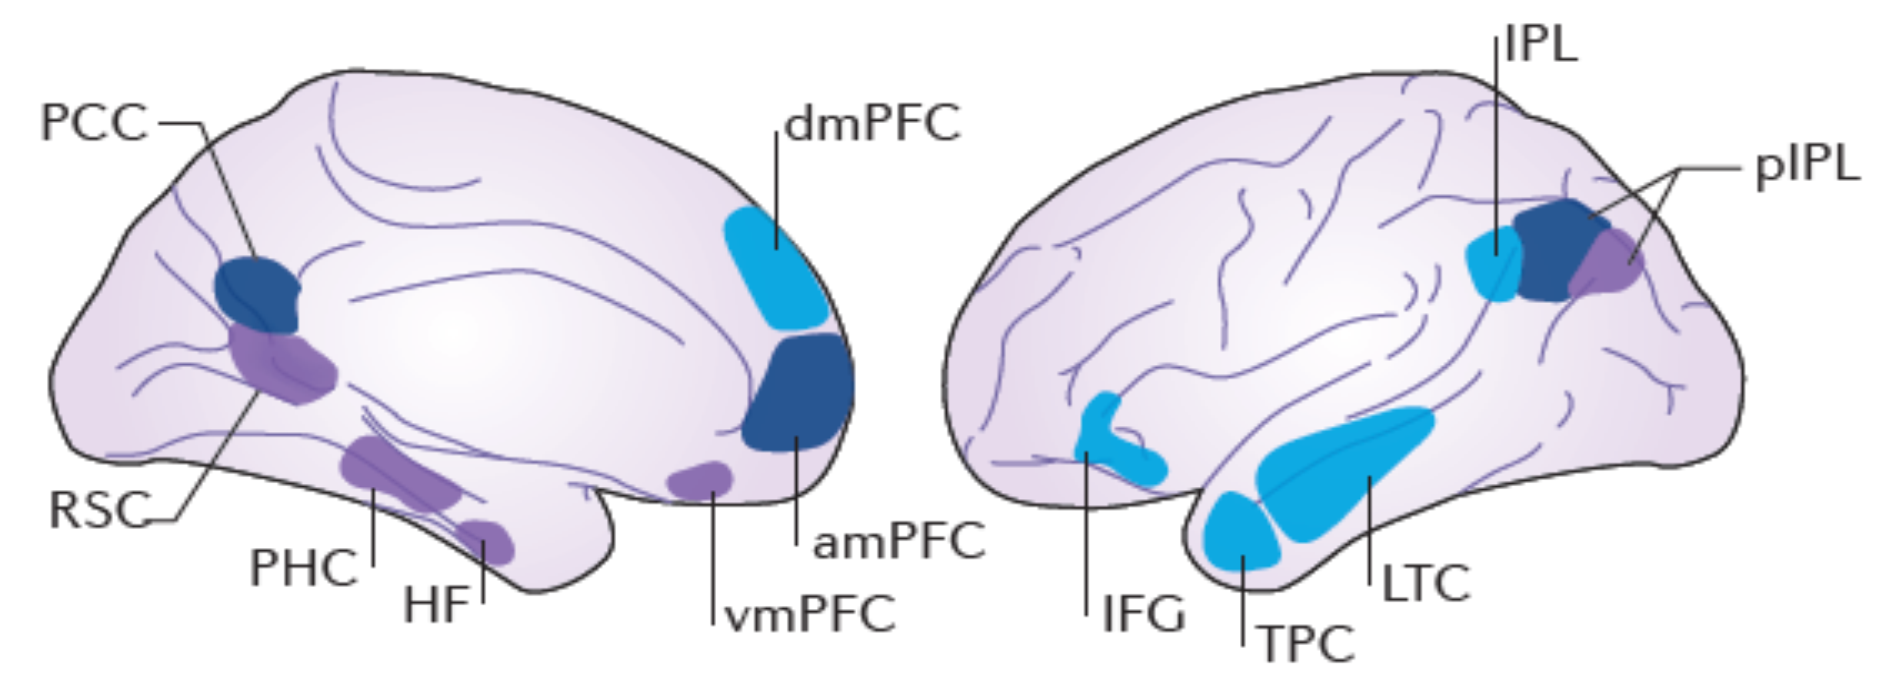
\includegraphics[width=0.9\textwidth]{Fig/Methods/fMRI_DMN/Intro_DMN.png}
	\caption[The default mode network and its subcomponents]{\textbf{The default mode network and its subcomponents}. The DMN is centered on the medial prefrontal cortex (MPFC), the medial parietal cortex and the lateral parietal cortex, and extends into the temporal lobe and lateral prefrontal cortex. Three subcomponents within the DMN have been identified. The first, the core DMN subsystem (deep blue) includes the MPFC, posterior cingulate cortex (PCC) and posterior inferior parietal lobule (pIPL). It is characterized by its hub-like properties and its contributions to internally oriented cognition. The second subcomponent (purple), which is known for its roles in memory and mental simulation, is centered on the medial temporal lobe (MTL), and includes as well the hippocampal formation (HF) and parahippocampal cortex (PHC). The third subcomponent (cyan) extends more dorsally and includes the dorsomedial prefrontal cortex (dmPFC), the lateral temporal cortex (LTC), the temporopolar cortex (TPC) and parts of the inferior frontal gyrus (IFG). It seems to be linked to a wide range of functions, including mentalizing, conceptual processing and emotional processing. Originally published in \citet{christoff_mind-wandering_2016}.}
	\label{fig:methods:dmn}
\end{figure}

\subsection{Anti-correlations between networks}
\label{sec:fmri:fc:anti-correl}

\citet{fox_human_2005} reported that the DMN is negatively coupled (anti-correlated) to brain networks involved in focused external visual attention (i.e. mainly the DAN). In other words, when the spontaneous BOLD fluctuations increase in the DMN, they decrease in the DAN. This dynamic interplay between two large, spatially distributed networks representing a priori opposing components of our mental lives (the DMN is involved in internal mental processes, while the DAN is involved in external attention) may \q{mark a fundamental feature of brain organization that had not been appreciated by earlier techniques} \citep{buckner_opportunities_2013}. Remarkably, a decrease anti-correlation between the DMN and the DAN has been consistently reported in a variety of altered vigilance states such as during NREM sleep (review in \citealp{picchioni_sleep_2013}) and after total sleep deprivation \citep{de_havas_sleep_2012}. This suggests that anti-correlation between these networks is an essential part of the brain normal functional organization.

\section{Resting-state fMRI data analysis}
\label{sec:fmri:rs}

The aim of this section is to provide a brief overview of the numerous processing steps that must be performed to go from the raw structural and functional MRI images to the group-level statistical analysis. These steps are summarized in Fig \ref{fig:methods:fmri-pipeline}.

\subsection{Preprocessing}
\label{sec:fmri:rs:preproc}

Steps in the spatial preprocessing of task-related and resting state fMRI data are similar. The first step is usually slice-timing correction, which aims at correcting temporal offset between slices within a repetition time by applying a temporal data interpolation to each voxel of the brain. Indeed, an fMRI scanner typically requires 2 seconds (i.e. repetition time or TR) to construct a full 3D brain volume by slicing the brain into multiple 2D layers (acquired either in ascending or interleaved order). Consequently, the BOLD signal (hemodynamic response) acquired in the last slice (late in the TR) peaks earlier than those in the slices acquired early in TR, even though the underlying activity is identical. Slice-timing correction applies a temporal data interpolation to each voxel of the brain in order to reconstruct a signal as if all the slices within a TR were acquired at the same exact time point.
The second main step is the coregistration which refers to the alignment of functional and structural images from the same subject to map functional information into anatomical space. In layman’s term, this step ensures that the brain images acquired from a single individual are always in the same position and space. This step is particularly important in resting-state fMRI due to the global effect of head movements on spontaneous BOLD fluctuations.
Next comes normalization, which refers to the spatial transformation of individual brains into a common space (typically Montreal Neurological Institute (MNI) space), a step crucial in order to make brain volumes acquired in different subject with different brain morphologies comparable to each other. A temporal filtering is sometimes applied to remove or attenuate frequencies within the raw signal that are not of interest. For instance, as functional connectivity fMRI studies the spontaneous low-frequency BOLD fluctuations, a bandpass filter on frequencies between 0.01 Hz - 0.1 Hz is usually applied. Finally, the last preprocessing step is generally the spatial smoothing, which aims at further increasing the signal-to-noise ratio by filtering out high frequency regions. Smoothing is a prerequisite to parametric statistical analysis (such as the Gaussian random fields) which assume that data are well-modeled by a normal distribution, however, there is a controversy as to the role of smoothing in resting-state fMRI (and notably graph analysis) in which increased spatial dependency introduced by smoothing might confound local connectivity strength \citep{hayasaka_comparison_2010}.

\begin{figure}[!htb]
	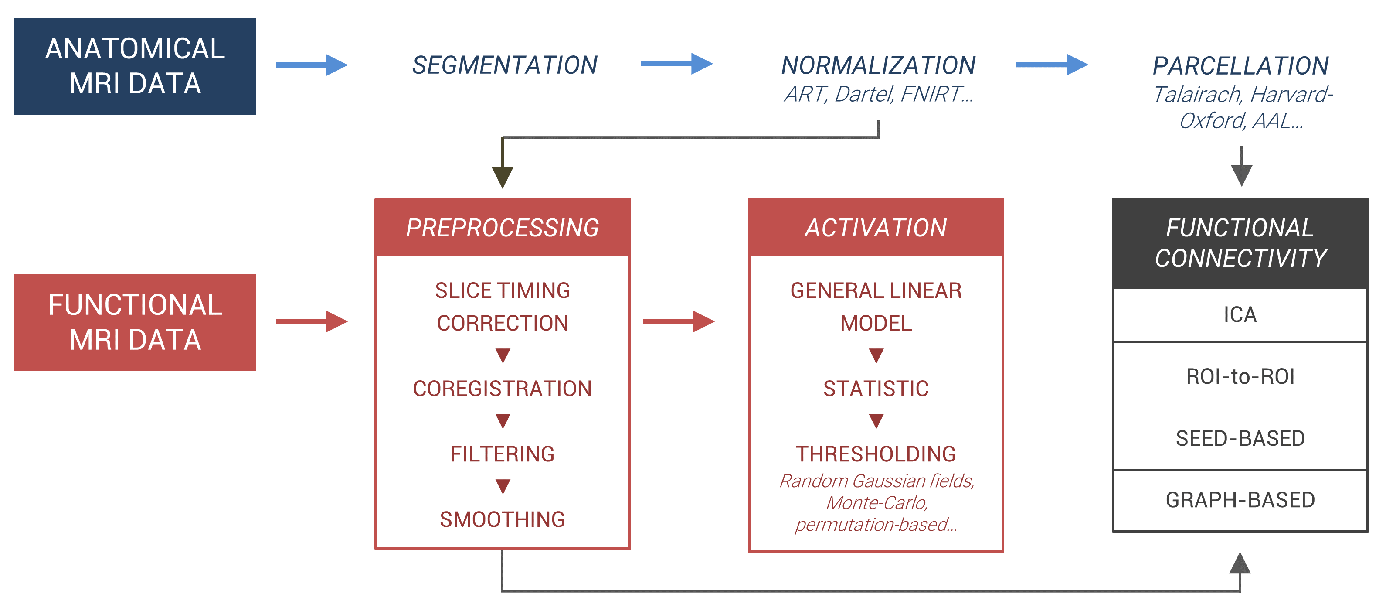
\includegraphics[width=\textwidth]{Fig/Methods/fMRI_pipeline/fMRI_pipeline_perso.png}
	\caption[Overview of the fMRI processing pipeline]{\textbf{Overview of the fMRI processing pipeline}. ICA = independent component analysis, ROI = regions of interests. Adapted from an original idea of Oussama Abdoun.}
	\label{fig:methods:fmri-pipeline}
\end{figure}

\subsection{Functional connectivity analysis}
\label{sec:fmri:rs:analysis}

There are three prominent methods to analyze preprocessed resting-state fMRI data (Fig \ref{fig:methods:ana-methods}). The first one is independent component analysis (ICA), which is a statistical method for separating a multivariate signal into additive subcomponents. Applied to brain functional connectivity data, it allows for example to separate distinct brain networks, without making any kind of initial assumptions \citep{beckmann_investigations_2005}. Because it requires no a priori defined regions of interests (ROIs), it can be quite easily implemented to identify brain networks or to remove noisy components of the signal (e.g. physiological noise, scanner drift). The second approach is based on a priori defined cluster of voxels (referred to as seeds, or ROIs). In this case, the signal from a specific seed is correlated either with all the other voxels of the brain (voxel-to-voxel approach) or others ROI (ROI-to-ROI approach). The ROI-to-ROI method is particularly well-suited to analyze within and between networks interactions, provided that the ROIs are defined a priori (for example using an ICA or a brain atlas). Finally, an emerging method in resting-state fMRI analysis is graph theory, which studies the spatio-temporal properties of brain networks using mathematical tools \citep{bullmore_complex_2009}.

\begin{figure}[htb]
	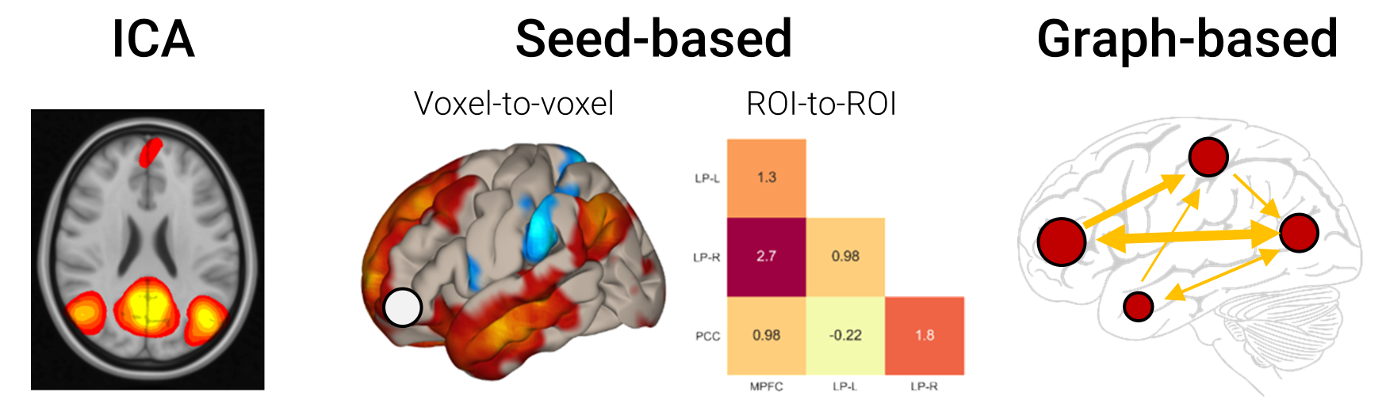
\includegraphics[width=\textwidth]{Fig/Methods/fMRI_seed_graph_ica/fMRI_seed_graph_ica.png}
	\caption[The three main methods of resting-state fMRI data analysis]{\textbf{The three main methods of resting-state fMRI data analysis}. (1) ICA is a highly data-driven method which is typically used to identify brain networks (in this example, the core regions of the DMN) or remove noisy components. (2) Seed-based connectivity requires one or several regions of interests (ROIs) to be a priori defined in order to compute the correlations between the seed regions and all the others voxels in the brain (voxel-to-voxel) or between specific ROIs (ROI-to-ROI). In this example, a symmetric correlation matrix was obtained by computing all the pairwise correlations within the DMN. (3) Graph-based connectivity studies the topological features of brain networks, which are defined in this context as a set of nodes (ROIs) linked by connections (edges). Using mathematical tools, several parameters can be computed such as the global efficiency and the level of modularity / clustering.}
	\label{fig:methods:ana-methods}
\end{figure}

\subsection{Combined EEG-fMRI recordings}
\label{sec:fmri:rs:eeg-fmri}

Simultaneous recording of EEG and MRI allow researchers to benefit from the excellent temporal resolution of EEG combined with the high spatial accuracy of fMRI. Applied to sleep, it allows for example to perform correlation between sleep features (detected using classic EEG-based criteria), and BOLD-fMRI signal \citep{duyn_eeg-fmri_2012}. The EEG can also be used to detect online the different sleep stages, thus allowing the experimenter to decide when to launch an fMRI scan. Simultaneous EEG-fMRI is therefore a valuable tool for investigating brain function across the spectrum of vigilance states.
However, there are a number of technical challenges that need to be overcome in order to improve EEG-fMRI data acquisition. Most importantly, EEG signals acquired during simultaneous fMRI are affected by several artefacts, namely the gradient artefact (caused by the changing magnetic fields gradients required for fMRI) and the cardio-ballistic artefact (linked to cardiac pulsations). Fortunately, these artefacts can be almost entirely removed, a posteriori but also in real-time, using dedicated softwares or algorithms.


\cleardoublepage
\part{EXPERIMENTAL RESULTS}
% !TEX root = ../thesis-example.tex
%
\chapter{The role of arousals on DRF variability}
\label{res:arousal}

\cleardoublepage

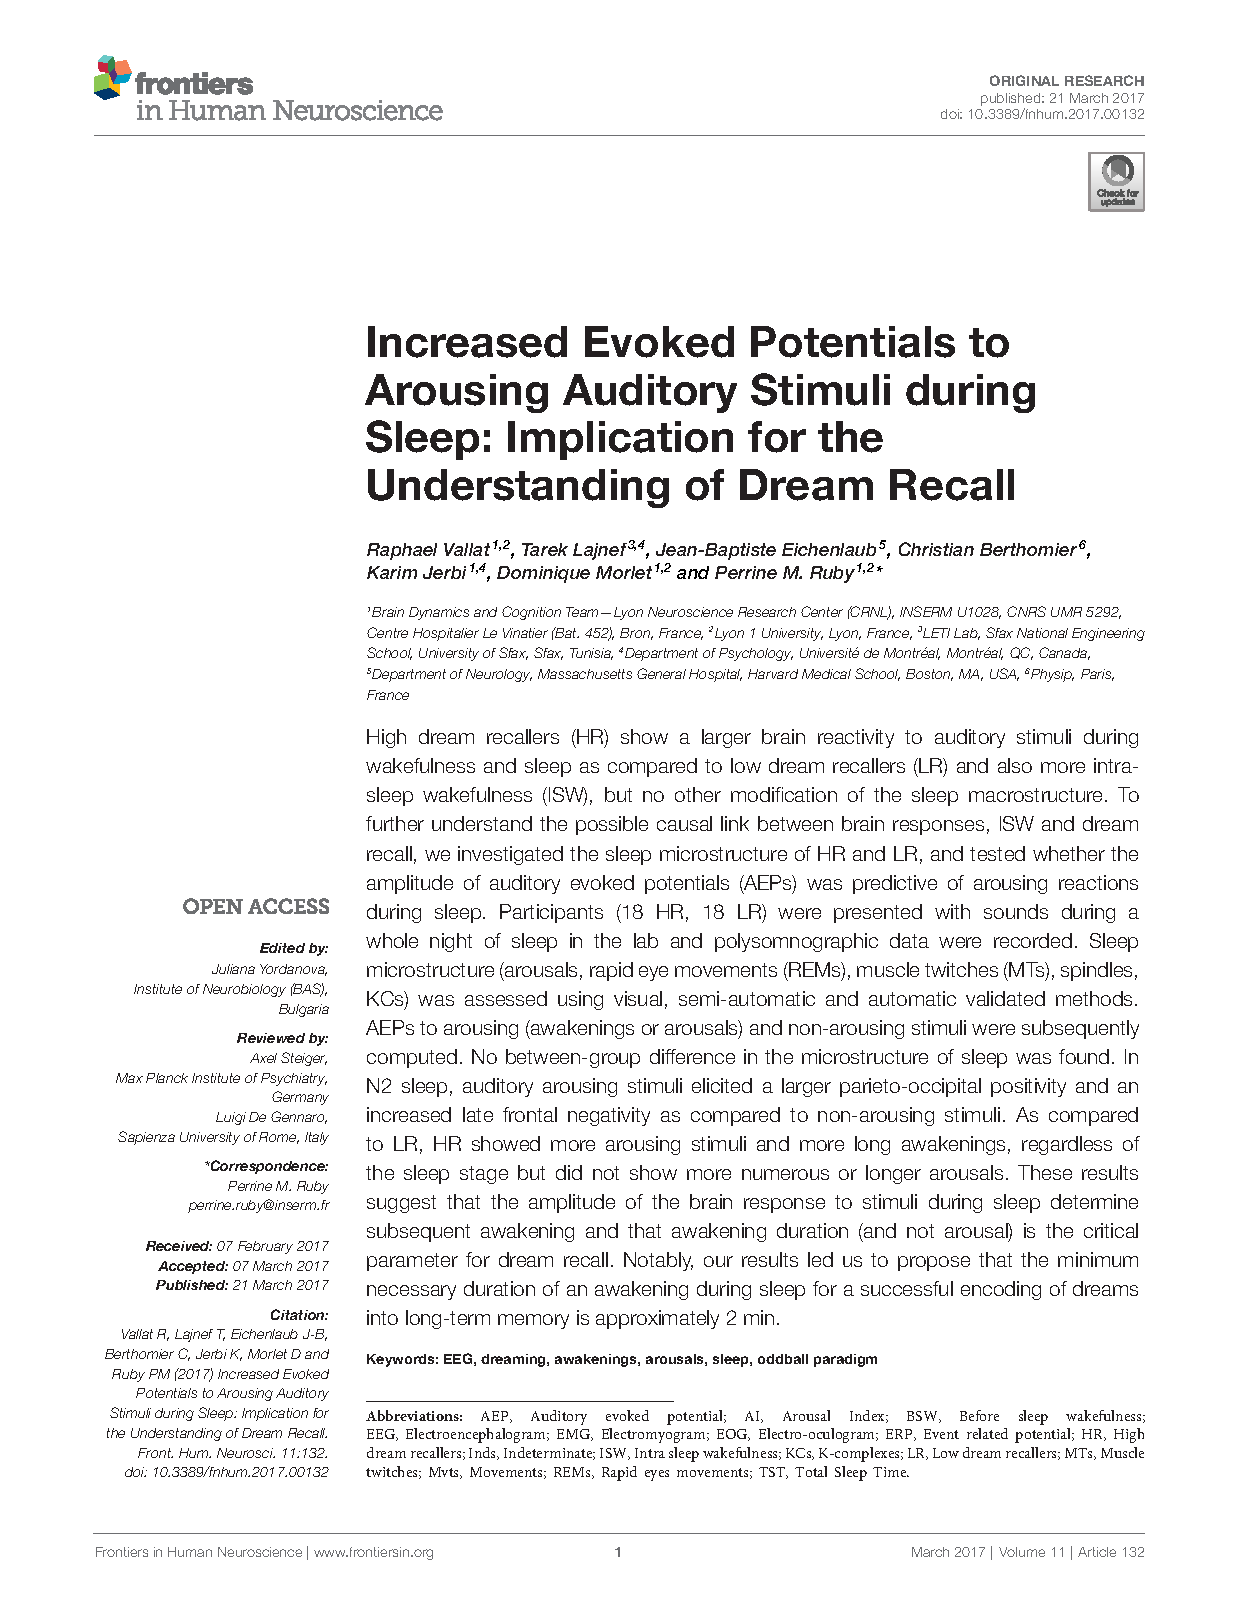
\includepdf[pages=-, pagecommand={\thispagestyle{plain}}]{Articles/Vallat_2017_FHN.pdf}

\cleardoublepage

\chapter{Study 2}
\label{res:inertia}

\section{Brain networks dynamics during sleep inertia}
\label{res:inertia:inertia}

\bigskip

\textbf{{\large Reduced default mode network connectivity and anti-correlation in the minutes following awakening from N2 and N3 sleep: an EEG-fMRI study}}

\hfill Under review at \emph{Neuroimage}

\bigskip

Raphael Vallat\textsuperscript{1} (PhD candidate), David Meunier\textsuperscript{1} (PhD), Alain Nicolas\textsuperscript{1,2} (M.D, PhD), Perrine Ruby\textsuperscript{1} (PhD)

\textsuperscript{1} Lyon Neuroscience Research Center, Brain Dynamics and Cognition team, INSERM UMRS 1028, CNRS UMR 5292, Université Claude Bernard Lyon 1, Université de Lyon, Lyon, France

\textsuperscript{2} Unité Michel Jouvet, Centre Hospitalier Le Vinatier, 95 boulevard Pinel, Lyon, France

\subsection*{Summary}
\label{res:inertia:inertia:summary}

The transition from sleep to wake is characterized by reduced vigilance, sleepiness and impaired performances, a state often referred to as sleep inertia. Even though the behavioral aspects of sleep inertia are well documented, its cerebral correlates remain poorly understood. Using combined EEG-fMRI in 55 participants, we examined the brain functional connectivity during sleep inertia before and after a 45 minutes mid-afternoon nap. Resting-state scans were acquired before the nap, 5 min and 25 min after awakening from N2 sleep (n=14) or N3 sleep (n=20). Results showed that sleep inertia is associated with an intrusion of sleep specific functional connectivity into wakefulness, which severity is dependent of the prior sleep duration and sleep depth. Awakening in N3 sleep induced the most robust changes and was characterized by a loss of brain functional segregation between task-negative and task-positive networks.

\paragraph{Keywords}
Sleep inertia, awakening, default mode network, combined EEG-fMRI, functional connectivity, dorsal attention network

% \subsection*{Abbreviations}
% \label{res:inertia:inertia:abbr}
% rCBF: regional cerebral blood flow, fMRI: functional magnetic resonance imaging, DMN: default mode network, DAN: dorsal attention network, FP: frontoparietal control network, SM: sensorimotor network, NREM: non rapid eye movement sleep, DST: descending subtraction task

\subsection*{Introduction}
\label{res:inertia:inertia:intro}

Sleep inertia is defined as a transient period occurring just after awakening from sleep, and characterized by reduced vigilance, sleepiness and impaired cognitive and physical performances \citep{tassi_sleep_2000, trotti_waking_2016}. As Trotti clearly pointed out in the title of her article \q{waking up is the hardest thing I do all day}, sleep inertia is also usually experienced as unpleasant. Although its duration is not consensual and varies depending on the outcome measure used, it is generally admitted that most of the behavioral effects of sleep inertia dissipate progressively in the first 30 minutes post awakening. Severity of sleep inertia has been positively associated to several factors such as prior sleep deprivation, awakening near the circadian trough of body temperature, awakening in slow-wave sleep (see \citet{tassi_sleep_2000} for a review) and some sleep disorders. Excessive sleep inertia, sometimes referred to as sleep drunkenness, is indeed a core feature of idiopathic hypersomnia and a component of delayed sleep phase disorder and NREM arousal parasomnias \citep{trotti_waking_2016}.

A better understanding of sleep inertia is needed for the development of new strategies to reduce its detrimental effects on cognitive and physical performances, in pathological or physiological context alike. Sleep inertia may indeed have critical consequences in emergency situations when individuals are required to make vital decisions or actions immediately upon awakening (e.g. medical staff, firemen, pilots, military). In the general population, sleep inertia represents the main limiting factor to the numerous beneficial effects of daytime napping \citep{faraut_napping:_2016}.

The behavioral aspects of sleep inertia are well documented, but only a limited amount of studies investigated its cerebral correlates until now. Using EEG, some studies have found a persistence of slow wave activity in the minutes following awakening, specifically in posterior areas, a phenomenon which has been suggested to represent the electrophysiological signature of sleep inertia \citep{ogilvie_falling_1992, ferrara_electroencephalographic_2006, marzano_recalling_2011, gorgoni_eeg_2015}. Using PET, \citet{balkin_process_2002} reported that the brain areas whose regional cerebral blood flow (rCBF) was increasing between 5 to 20 min post awakening (p-a) were primarily anterior heteromodal areas (e.g. lateral prefrontal cortices, and anterior insula). They also reported shifts in the relative levels of rCBF between pairs of brain regions (orbitofrontal cortex and ventromedial caudate nucleus, dorsolateral prefrontal cortex and mesencephalic reticular formation) between 5 and 20 min post awakening, leading them to propose that recovery from sleep inertia could hinge on a resumption of normal levels of both rCBF and functional connectivity between brain areas. The latter hypothesis has been tested in two recent resting-state functional magnetic resonance imaging (fMRI) studies which investigated the variations in brain connectivity between pre-sleep wakefulness, nocturnal sleep (without previous sleep deprivation) and post-sleep wakefulness \citep{wu_variations_2012, tsai_local_2014}. Using paired comparisons between pre- and post-sleep wakefulness, they found a decreased connectivity within the sensory-motor (SM) network at awakening but no alterations in the default mode network (DMN). This altered connectivity within the sensory-motor network is coherent with the poor motor performances observed at awakening but does not explain the impairments observed in other domains (e.g. cognitive tasks such as mental calculation, \citealp{tassi_sleep_2000, trotti_waking_2016}).

Some modifications of the DMN connectivity could be expected at awakening since several neuroimaging studies showed consistent alterations of the DMN connectivity during sleep, fatigue and/or falling asleep (see \citet{picchioni_sleep_2013} for a review). During N1 and N2 sleep, several teams found a decrease in the anti-correlation between the default mode network on one hand and task-positive networks on the other (i.e. dorsal attention and executive control networks). This decreased anti-correlation has also been observed during wake after total or partial sleep deprivation, in addition with robust alterations across the whole brain functional connectome \citep{samann_increased_2010, de_havas_sleep_2012, yeo_functional_2015, kaufmann_brain_2015, tushaus_resisting_2017}. Finally, during deep sleep (N3 or slow-wave sleep), several studies reported a strong disruption of DMN connectivity and anti-correlation \citep{horovitz_decoupling_2009, larson-prior_modulation_2011, samann_development_2011}, as well as an absence of frontoparietal connectivity \citep{spoormaker_frontoparietal_2012}). Altogether, these results argue in favor of a progressive loss of functional segregation of brain networks from sleep onset to deep sleep, which might explain why the behavioral impairments at awakening are the most acute when individuals are awakened in N3 sleep and lead to the hypothesis that awakening from N3 sleep should be associated with DMN functional connectivity disruption.

In order to improve our understanding of sleep inertia, we designed a study with several novelties compared to previous ones. First, we used a combined EEG-fMRI method to acquire resting state scans before sleep, 5 min after awakening and 25 min after awakening in 55 healthy young participants. This design enabled us to investigate the dynamic of functional connectivity in several brain networks during the first half hour following awakening. Second, participants were partially sleep deprived on the night before and awakened from a 45 min mid-afternoon nap, in the deepest possible sleep stage (N3 sleep). Both sleep deprivation and awakening in N3 sleep have been associated with increased sleep inertia \citep{tassi_sleep_2000}. In addition with being ecological (short nights compensated by a daytime nap being common in young adults \citep{faraut_napping:_2016}, this paradigm allowed us to study sleep inertia in its most intensified form. Finally, each resting-state scan was paired with a mental calculation task in order to measure the behavioral effects of sleep inertia.

Using such a design we aimed at characterizing the brain functional connectivity just after awakening from deep sleep (N3) and its modulation in the first half hour after awakening. A total of 55 participants were included, of which 20 were awakened in N3 sleep and 14 in N2 sleep, allowing us to describe and compare the functional connectivity during sleep inertia following awakening from these two distinct sleep stages.

We expected a decrease in performances 5 min p-a compared to pre-sleep and 25 min p-a. We hypothesized that (1) the functional connectivity 5 min after awakening would share some features with the one of the sleep stage that was ongoing before awakening, i.e. we notably expected to observe a decrease in DMN connectivity and anti-correlation after awakening from N2 or N3 sleep (2) a decreased connectivity within the SM network (3) a positive correlation between the severity of performance impairments and functional connectivity disruption at awakening on the one hand and sleep depth before awakening on the other hand.

\subsection*{Methods}
\label{res:inertia:inertia:methods}

\subsubsection*{Participants}
Fifty-five participants (28 males, mean age = 22.55, standard deviation = 2.41, range = 19–29) were included in the study. The subjects were informed of the study through an announcement sent to several mailing lists of Lyon University. Participants were selected if they reported having a regular sleep-wake schedule, no difficulty to fall asleep, being occasional or frequent nappers and having preferentially already done an MRI brain scan in the past few years. They had no history of neurological and psychiatric disorders, and had no sleep disturbances. They provided written informed consent according to the Declaration of Helsinki and received monetary compensation for their participation. The study was approved by the local ethics committee (CCPPRB, Centre Leon Berard, Lyon, France).

\subsubsection*{Experimental design}
The experimental design is presented in Fig 1 (see Fig \ref{fig:intro:problematics-fmri-paradigm}).

% \begin{figure}[htb]
% 	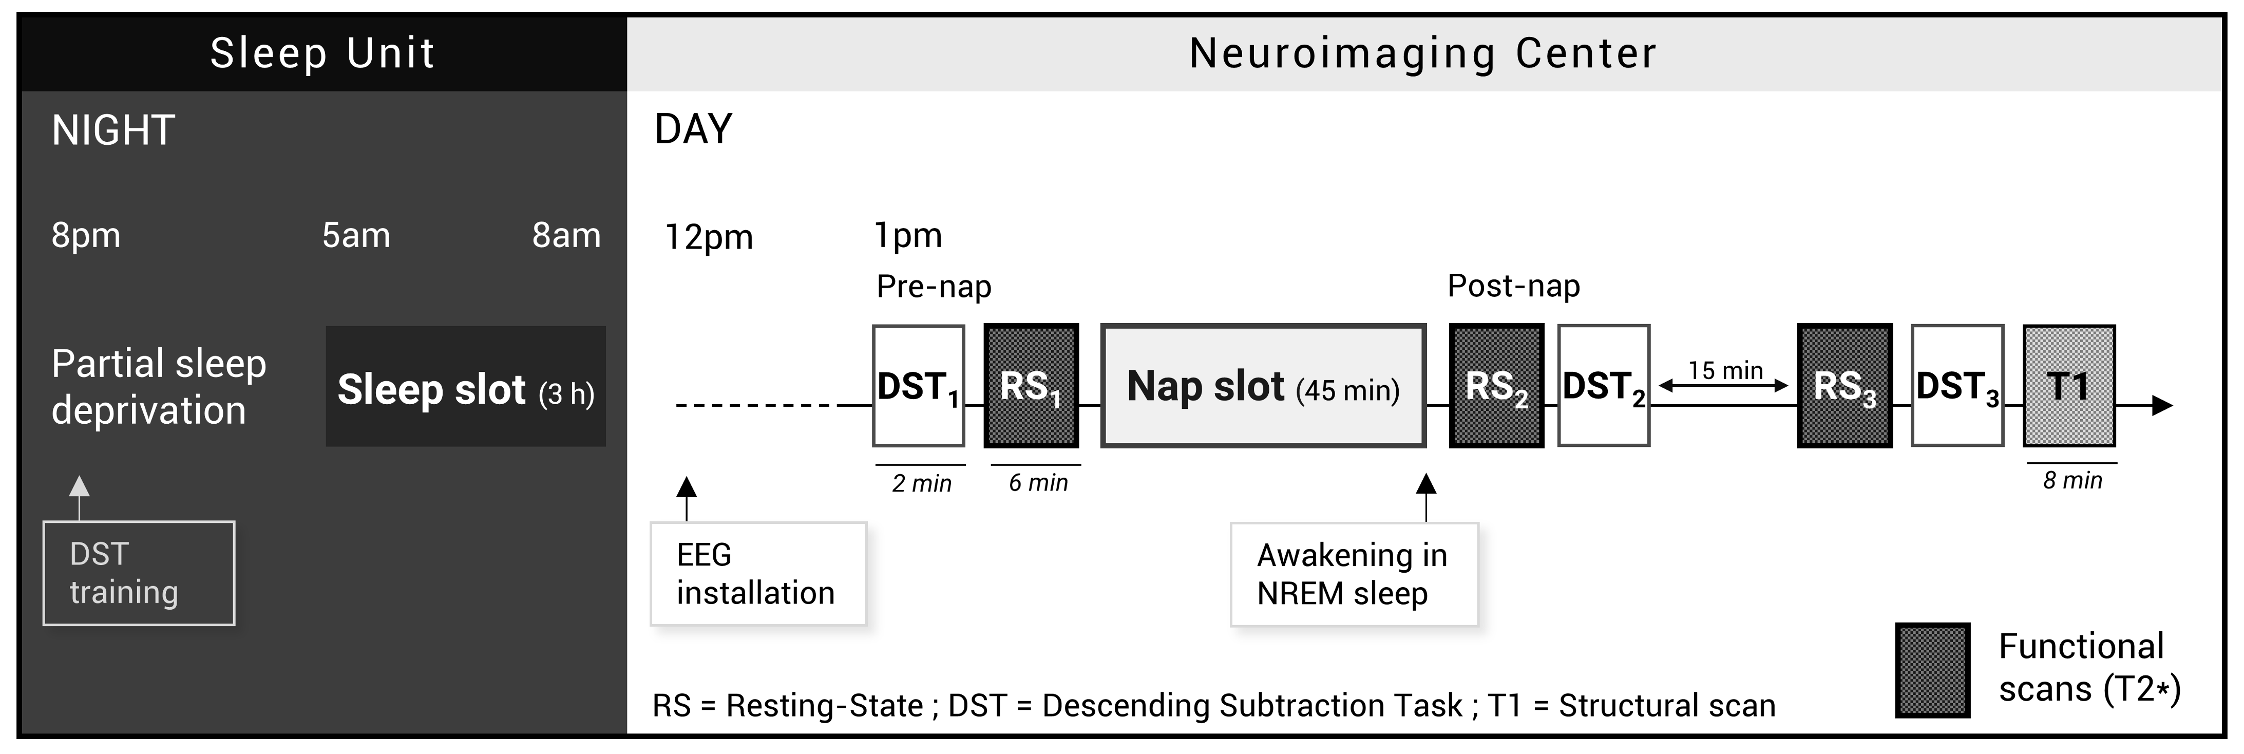
\includegraphics[width=\textwidth]{Fig/Results/Inertia/Inertia/Fig1_Protocol.png}
% 	\caption*{\textbf{Fig 1. Experimental design}}
% \end{figure}

\emph{Evening and night}. Participants arrived in the sleep unit of the hospital Le Vinatier (Lyon, France) at 8 pm on the evening prior to the experimental day. From 8 pm to 10 pm, they underwent several personality and cognitive tests (results will be presented elsewhere) administered by R.V. They were then instructed to stay awake until 5 am (the possible activities were reading, making puzzles and watching movies), at which point they were allowed to sleep for 3 hours until 8 am in a bed in the sleep unit. Energy drinks or physical activity were prohibited during the partial sleep deprivation, and nurses regularly checked that the subject did not fall asleep. The monitoring of body movements through wrist actigraphy (Actigraph, Pensacola, USA) during the whole night made it possible to check a posteriori that the subject did not fall asleep before 5 am. In the morning, participants were offered breakfast and a shower and then occupied themselves (reading or internet) under the experimenters’ supervision until the MRI session.

\emph{Day}. After lunch at 11.30 am, participants were conducted to the neuroimaging center (CERMEP). During the first half hour, experimenters installed on the participant’s head a MRI compatible EEG cap (EASYCAP®). Participants were then installed in the MRI scanner at about 1.20 pm (1.17 pm ± 13 min). They read a 5 min cartoon during the calibration of the eye-tracking camera, and then did the DST for 2 minutes. The first resting-state scan was then acquired, with the instructions to remain awake and look at a central fixation cross on the screen. At the end of the scan, participants were informed that they could sleep (at 1.39 pm ± 14 min in average) during the next 45 min. At the end of the nap slot, participants were awakened, if they were sleeping, by calling their first name and the 2nd resting state scan was acquired in the following minutes. At the end of the scan, the 2nd DST was performed. During the following 10 minutes, questions about sleep in the scanner and about the cartoon were asked to the subjects (results will be reported elsewhere). Then the 3rd resting state scan and DST were performed (about 25 min after awakening). Finally, an 8-min T1 anatomical scan was acquired. When they got out of the MRI, participants completed a questionnaire about their thoughts during the three resting state scans.

\subsubsection*{Behavioral tasks}
To evaluate the time course of the dissipation of sleep inertia we used the descending subtraction task (DST) that has been previously used to evidence performances decrement and normalization in the first 30 min post awakening \citep{dinges_assessing_1985, evans_recovery_1975, stampi_ultrashort_1990}. Subjects were presented with a three-digit number. They were instructed to subtract 9, saying the operation and the result aloud, and then continue by subtracting 8 from the remainder, then 7, and so on until they had to subtract 1. At this point they were to start the cycle of descending subtractions again. They had to do the task for two minutes and were instructed to be as fast and accurate as possible. As this task has a substantial practice effect over the first trials \citep{dinges_assessing_1985}, participants were trained the night before the fMRI session (they performed the task six times during the evening in the sleep unit).

The outcome measures from the DST are: 1) the total number of responses, which is an index of the speed of information processing, 2) the percentage of mistakes, which is a marker of accuracy, 3) the percentage of correct responses (relative to pre-nap performances), which is a marker of both speed and accuracy \citep{dinges_assessing_1985}. Since several studies reported that speed is generally more impaired than accuracy during sleep inertia \citep{trotti_waking_2016}, we expected a significant decrement of post-nap performances especially for the total number and percentage of responses.

\subsubsection*{EEG data collection}
Polysomnography data were recorded using a 15 channels MR-compatible cap designed for sleep studies i.e. with a layout designed according to American Academy of Sleep Medicine Guidelines 2007 (EasyCap, Brain Products GmbH, Gilching, Germany). It comprised 9 EEG electrodes placed according to the international standard 10/20 system (O1, O2, C3, C4, F3, F4, M1, M2, Cz, FCz was used as reference and AFz as ground), 2 EOG electrodes, 3 EMG electrodes, and an electrocardiogram electrode placed on the back of the participant. The sampling rate was 5000 Hz and an analog band-pass filter was set to 0.01 – 250 Hz. To score sleep online during the fMRI session, a real-time pulse-artefact correction was applied using the BrainVision Recorder (Version 1.2) and BrainVision RecView (Version 1.4) softwares (Brain Products).

To ensure that participants were not closing their eyes during the resting state scans, eye movements were monitored during the experiment using an EyeLink 1000 fMRI eye tracking system (SR Research Ontario, Canada). Eye position was calibrated at the beginning of the experiment and monitored throughout.

\subsubsection*{MRI data collection}
MRI scans were obtained from a MAGNETOM Prisma 3.0 T scanner (Siemens Healthcare, Erlangen, Germany) at the Primage neuroimaging platform (CERMEP). Structural MRI were acquired with a T1-weighted (0.9-mm isotropic resolution) MPRAGE sequence and functional MRI data with a T2*-weighted 2D gradient echo planar imaging sequence (EPI) with 180 volumes (TR/TE: 2000/ 25 ms; flip angle: 80°; voxel size: 2.68 × 2.68 × 3 mm; slices: 40, duration: 6 minutes). Functional and anatomical scans were performed using a 20-channel head coil. The coil was foam-padded to improve subject comfort and restrict head motion.

\subsubsection*{EEG analysis}
Artifacts related to gradient switching and cardiac pulse (cardio-ballistic artifact) were removed using standard routines available in BrainVision Analyzer version 2.0 software (Brain Products). Polysomnographic data were downsampled to 1000 Hz and band-pass filtered between 0.5 and 25 Hz. Offline sleep stage scoring was performed using EEG epochs of 30 seconds following standard AASM rules (Iber, 2007; Silber et al., 2007) visualized using SLEEP software \citep{combrisson_sleep:_2017}. S1 Fig shows the hypnogram during the nap slot for one subject who reached N3 sleep.

\subsubsection*{fMRI analysis}
Preprocessing and quality check were performed using standard routine in SPM12 software (Wellcome Department of Imaging Neuroscience). Preprocessing included functional realignment, slice-time correction, coregistration to structural scan, spatial normalization and spatial smoothing using a 6 mm full-width at half-maximum isotropic Gaussian kernel filter. Individual T1 images were segmented into gray matter, white matter and cerebrospinal fluid tissue maps. Functional and structural images were then normalized to MNI152 space (Montreal Neurological Institute). Functional images underwent artifact and motion regression in the Artifact Detection Toolbox (\fnurl{ART}{https://www.nitrc.org/projects/artifact_detect/}) using the following criteria to define outliers: global signal intensity changes greater than 9 standard deviations and movement exceeding 2 mm. SPM motions parameters and outliers were subsequently included as covariates in connectivity analyses.

Resting-state networks and their main regions of interests (ROIs) were defined from a brain parcellation atlas implemented in the \fnurl{CONN Toolbox}{http://www.nitrc.org/projects/conn} version 17f \citep{whitfield-gabrieli_conn:_2012}. This atlas was obtained using an independent component analysis (ICA) on 467 subjects from the Human Connectome Project. Subcortical ROIs (hippocampus, thalamus, and amygdala) were defined from the Harvard-Oxford maximum likelihood subcortical atlas. Spatial maps of the ROIs used in further connectivity analyses for each network of interest are displayed in S2 Fig.

Connectivity analysis were performed using the CONN toolbox version 17f. First, we performed a denoising step including a regression of the 6 motion correction parameters and their corresponding first-order temporal derivatives, as well as a component-based strategy (aCompCor, \citealp{behzadi_component_2007}) to identify and remove physiological confounds that are unlikely to be related to neural activity. The resulting BOLD time series were band-pass filtered (0.008 – 0.09 Hz) to further reduce noise and increase sensitivity \citep{weissenbacher_correlations_2009}. Then, intra- and inter-network connectivity were calculated for each subject by extracting the mean BOLD time series of each ROI of a given network and by correlating them with the average BOLD time series of every other ROI from this network or of the other networks included in the analysis. The mean network connectivity was then computed as the mean of all pair-wise Fischer-transformed correlation coefficient within a network and compared within subjects between conditions and between subjects. In addition with the previously described ROI-to-ROI analysis, we performed seed-to-voxel analysis on the posterior cingulate cortex (PCC), one core region of the DMN which demonstrates notable disruption during NREM sleep (\citealp{picchioni_sleep_2013}; center of mass in MNI coordinates: 1, -61, 38).

\subsubsection*{Statistics}
For the descending subtraction task, between-group comparisons were achieved using a mixed two-way repeated measures ANOVA with a group factor (two levels: N2 sleep and N3 sleep, see results section) and a time factor (within subject factor with three levels: Pre-sleep, 5 min p-a, 25 min p-a). Post hoc analyses (t-tests) were used in case of significance. ROI-to-ROI connectivity analysis were conducted using two-sided t-tests corrected for multiple comparisons using the false discovery rate (FDR, p<.05). Seed-based connectivity analysis were performed using a cluster-defining voxel-wise height threshold of p<.01 (uncorrected, two-sided) and a whole-brain family-wise error (FWE) corrected extent threshold of p<.05.

\subsection*{Results}
\label{res:inertia:inertia:results}

\subsubsection*{Sleep parameters}
Despise the sleep deprivation, 20 out of 55 participants did not reach or maintain NREM sleep during the 45-min nap slot in the scanner. This result was not a surprise given the discomfort and stress inherent to the MR environment \citep{duyn_eeg-fmri_2012}. One subject out of the 35 remaining was discarded because of a technical failure during data acquisition, leading thus to a total of 34 participants included in the final analysis. We further divided these participants as a function of the sleep stages they were in before awakening. Twenty participants were awakened in N3 sleep (N3 group) and 14 participants were awakened in N2 sleep (N2 group). This allowed us to compare the functional connectivity during sleep inertia after awakening from both N2 and N3 sleep. Between-group comparisons were performed both for the functional connectivity and the behavioral data. Means of the main sleep parameters in the two groups are presented in Table 1. Importantly, there was no group difference in the latency between the awakening and the first and second post-awakening resting-state scan, respectively. Note that as expected, the sleep deprivation did succeed to maximize sleep inertia at awakening. Indeed a few participants experienced very difficult awakenings marked by a short period of panic, claustrophobia and blast of hot air, often accompanied by strong neurovegetative responses (tachycardia, hyperventilation, sudation).

\begin{table}[htb]
    \caption*{\textbf{Table 1. Sleep parameters (Mean ± SD) of the subjects in the N3 (n=20) and N2 (n=14) groups.} TST = Total Sleep Time, SE = Sleep Efficiency, Wake (W), N1, N2 and N3 = Total duration of each sleep stage in minutes. LAS1 = latency (min) between the awakening and the start of the first post-awakening resting-state scan. LAS2 = latency (min) between the awakening and the start of the second post-awakening resting-state scan.}
    \begin{tabularx}{\textwidth}{XXXXXXXXX}
    \toprule
    Group  & TST        & SE (\%)       & W         & N1         & N2         & N3          & LAS1      & LAS2 			\\ \midrule
    N2     & 38.2 ± 7.1 & 87.4 ± 9.6    & 9.1 ± 4.0 & 14.2 ± 7.6 & 21.6 ± 6.2 & 2.9 ± 4.4   & 3.7 ± 1.9 & 23.8 ± 3.7 	\\
    N3     & 37.3 ± 5.0 & 87.5 ± 7.4    & 9.2 ± 4.2 & 9.0 ± 5.7  & 17.7 ± 4.9 & 11.0 ± 4.6  & 4.8 ± 3.9 & 24.4 ± 4.2 	\\
    T-test & .68        & .99           & .95       & .03        & .05        & <.001       & .34       & .63 			\\ \bottomrule
    \end{tabularx}%
\end{table}

\subsubsection*{Descending subtraction task}
Performance at the DST during the fMRI session are presented in Fig 2. As expected, we observed a significant main effect of time [F(2, 32)=4.0, p=.02] in the total number of responses. The total number of response was lower at 5 min post-awakening as compared to 25 min post-awakening (p=.008 ; Fig 2A). There was a tendency for a reduced total number of responses at 5 min compared to pre-sleep (p=.07). No group effect or interaction were found for the total number of responses. This decrease in calculation speed at 5 min post-awakening was not associated with a significant increase in the percentage of mistakes (Fig 2B). This result is consistent with the generally held view that speed is more impaired than accuracy during sleep inertia (Trotti, 2016). However, there was a significant interaction between time and group factors [F(2,32)=3.60, p=.03]. Post-hoc tests revealed that the N2 group had a higher percentage of mistakes at 5 min post-awakening compared to the N3 group (p<.001). Finally, regarding the percentage of correct responses, which is a marker of both speed and accuracy, we also found a significant main effect of time [F(2, 32)=3.13, p=.05]. The number of correct responses was lower at 5 min post-awakening than at 25 min post-awakening (p=.01), but not significantly different before the nap as compared to 5 min after awakening (p=.17; Fig 2C). As for the total number of responses, no group effect or interaction was found for the percentage of correct responses.

\begin{figure}[htbp]
	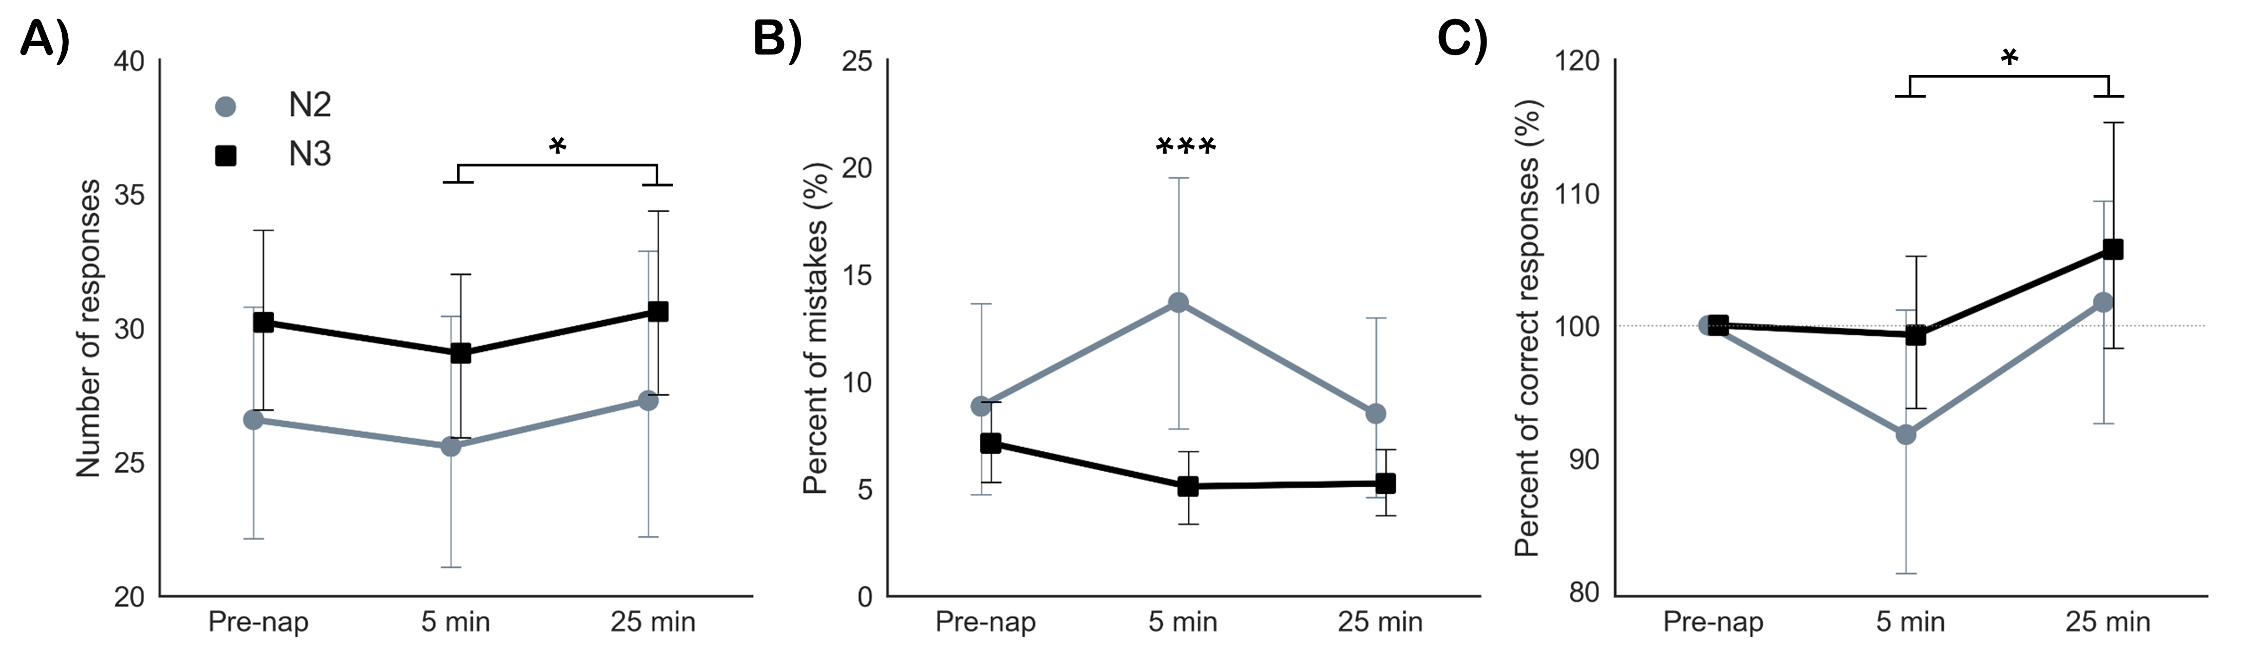
\includegraphics[width=\textwidth]{Fig/Results/Inertia/Inertia/Fig2_DST.png}
	\caption*{\textbf{Fig 2. Performances of the Descending Subtraction Task.} Blue gray lines, N2 group (n=14), black lines, N3 group (n=20). (A) Total number of responses (index of speed). (B) Percentage of mistakes (marker of accuracy). (C) Percentage of correct responses relative to pre-nap performances (marker of both speed and accuracy). Error bars represent 95\% confidence intervals. * p<.05, *** p<.001}
\end{figure}

\subsubsection*{Functional connectivity alterations following awakening from N3 sleep}
The brain functional connectivity at 5 min after awakening from N3 sleep showed important alterations. ROI-to-ROI analysis demonstrated a disrupted pattern of connectivity between several brain networks at 5 min p-a compared to pre-nap and 25 min p-a. Fig 3A illustrates the connectivity between several network, notably the DMN, DAN, fronto-parietal executive network (FP), sensori-motor (SM), salience and visual networks, in the pre-nap and 25 min p-a conditions as compared to the 5 min p-a condition. Fig 3B shows mean pairwise connectivity within and between networks. One of the most significant result was the large decrease of the anti-correlation (i.e. increased connectivity between networks that are normally anti-correlated) at 5 min p-a between the DMN and several other networks, namely the DAN, the SM, and the salience networks (Fig 3A and 3B, right). Interestingly, we observed alterations in the between-networks functional connectivity, whereas the mean within-network functional connectivity within each of these networks was not reduced at 5 min p-a compared to the two other conditions (Fig 3B, left). Seed-based analysis confirmed the disruption of the anti-correlation between the DMN (seed in the PCC) and SM network at 5 min p-a compared to pre-sleep and 25 min p-a (Fig 3C and S1 Table). In addition, there was a reduced connectivity at 5 min p-a compared to pre-sleep between the PCC and the inferior temporal gyrus, a region considered to be a part of the extended DMN and known for its role in memory and mental simulations \citep{christoff_mind-wandering_2016}.

\begin{figure}[!htbp]
	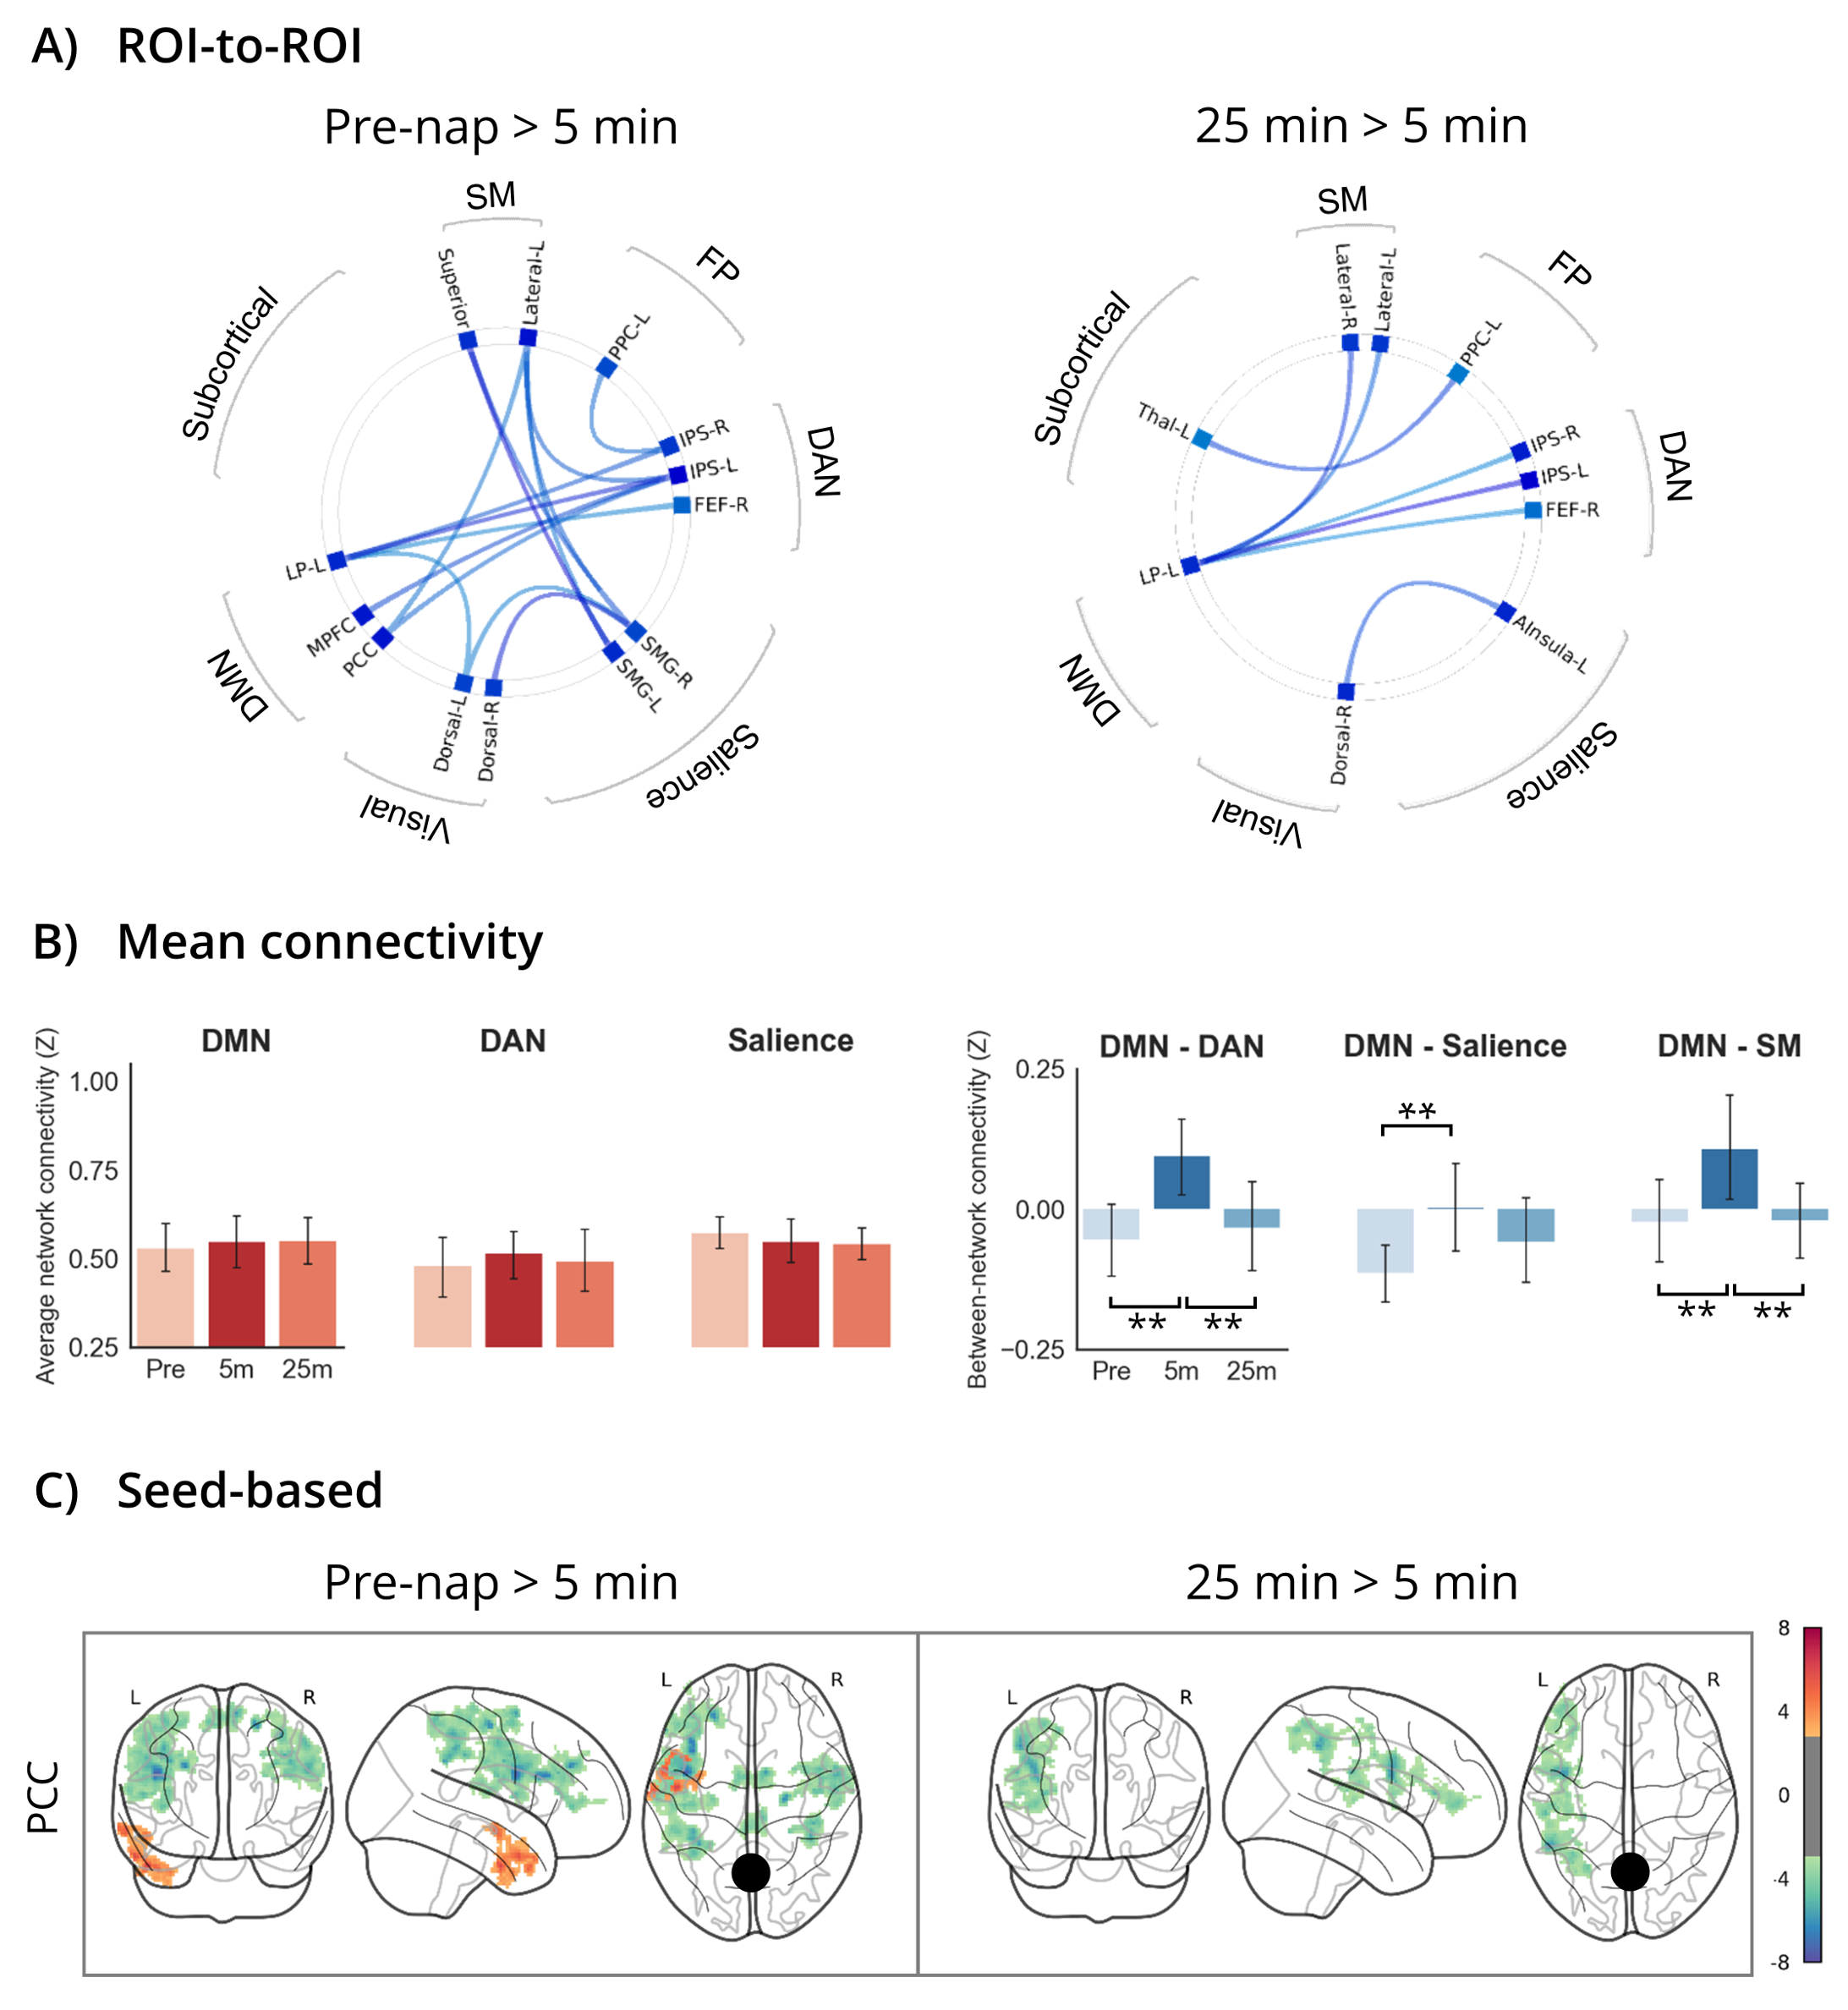
\includegraphics[width=\textwidth]{Fig/Results/Inertia/Inertia/Fig3_N3.png}
	\caption*{\textbf{Fig 3. Functional connectivity disruption after awakening from N3 sleep (n=20)}. (A) ROI-to-ROI results for the two contrasts (left, Pre-nap minus 5 min p-a; right, 25 min p-a minus 5 min p-a). Blue connections indicate regions with significantly increased pairwise connectivity (two-sided paired t-test, p<.05 FDR-corrected) at 5 min p-a compared to the pre-nap condition (left) and compared to the 25 min p-a condition (right). (B) Mean pairwise connectivity within (left, red bars) and between (right, blue bars) networks. Stars denote significant post-hoc comparisons (t-tests, ** p<.01). (C) Seed-based connectivity results for the two contrasts (left, Pre-nap minus 5 min p-a; right, 25 min p-a minus 5 min p-a). Seed region is the posterior cingulate cortex (PCC), one core region of the DMN which demonstrates notable disruption during NREM sleep (center of mass in MNI coordinates: 1, -61, 38). Statistical parametric maps are reported using an uncorrected two-sided cluster-defining voxel-wise height threshold of p<.01 and a whole-brain FWE-corrected extent threshold of p<.05. Yellow-red colors indicate increased connectivity at pre-nap and/or 25 min p-a compared to the 5 min p-a scan. Green-blue colors indicate increased connectivity at 5 min p-a compared to the two other scans.}
\end{figure}

\subsubsection*{Functional connectivity alterations following awakening from N3 sleep}
Awakening from N2 sleep was also associated with some alterations in the brain connectivity. As compared to pre-sleep, the functional connectivity at 5 min p-a was reduced between the SM and two regions of the FP network, the SM and the right hippocampus and between the ventral and dorsal part of the visual network. By contrast, the connectivity at 5 min p-a was increased between two regions of the DMN and the hippocampus and between the salience and SM networks (Fig 4A). As compared to 25 min p-a, the functional connectivity at 5 min p-a was reduced within the DAN, within the ventral and dorsal part of the visual network, and between the SM and FP networks. By contrast, connectivity was increased between the visual and salience networks (Fig 4A). The mean connectivity within and between networks was not significantly altered at 5 min p-a after an awakening in N2 sleep (Fig 4B). In accordance with these results, seed-based analysis showed an increased connectivity at 5 min-pa compared to pre-sleep between the PCC and several regions including the hippocampus and part of the SM network (Fig 4C and S2 Table). PCC connectivity was not significantly different at 25 min p-a compared to both pre-sleep and 5 min p-a.

\begin{figure}[!htbp]
	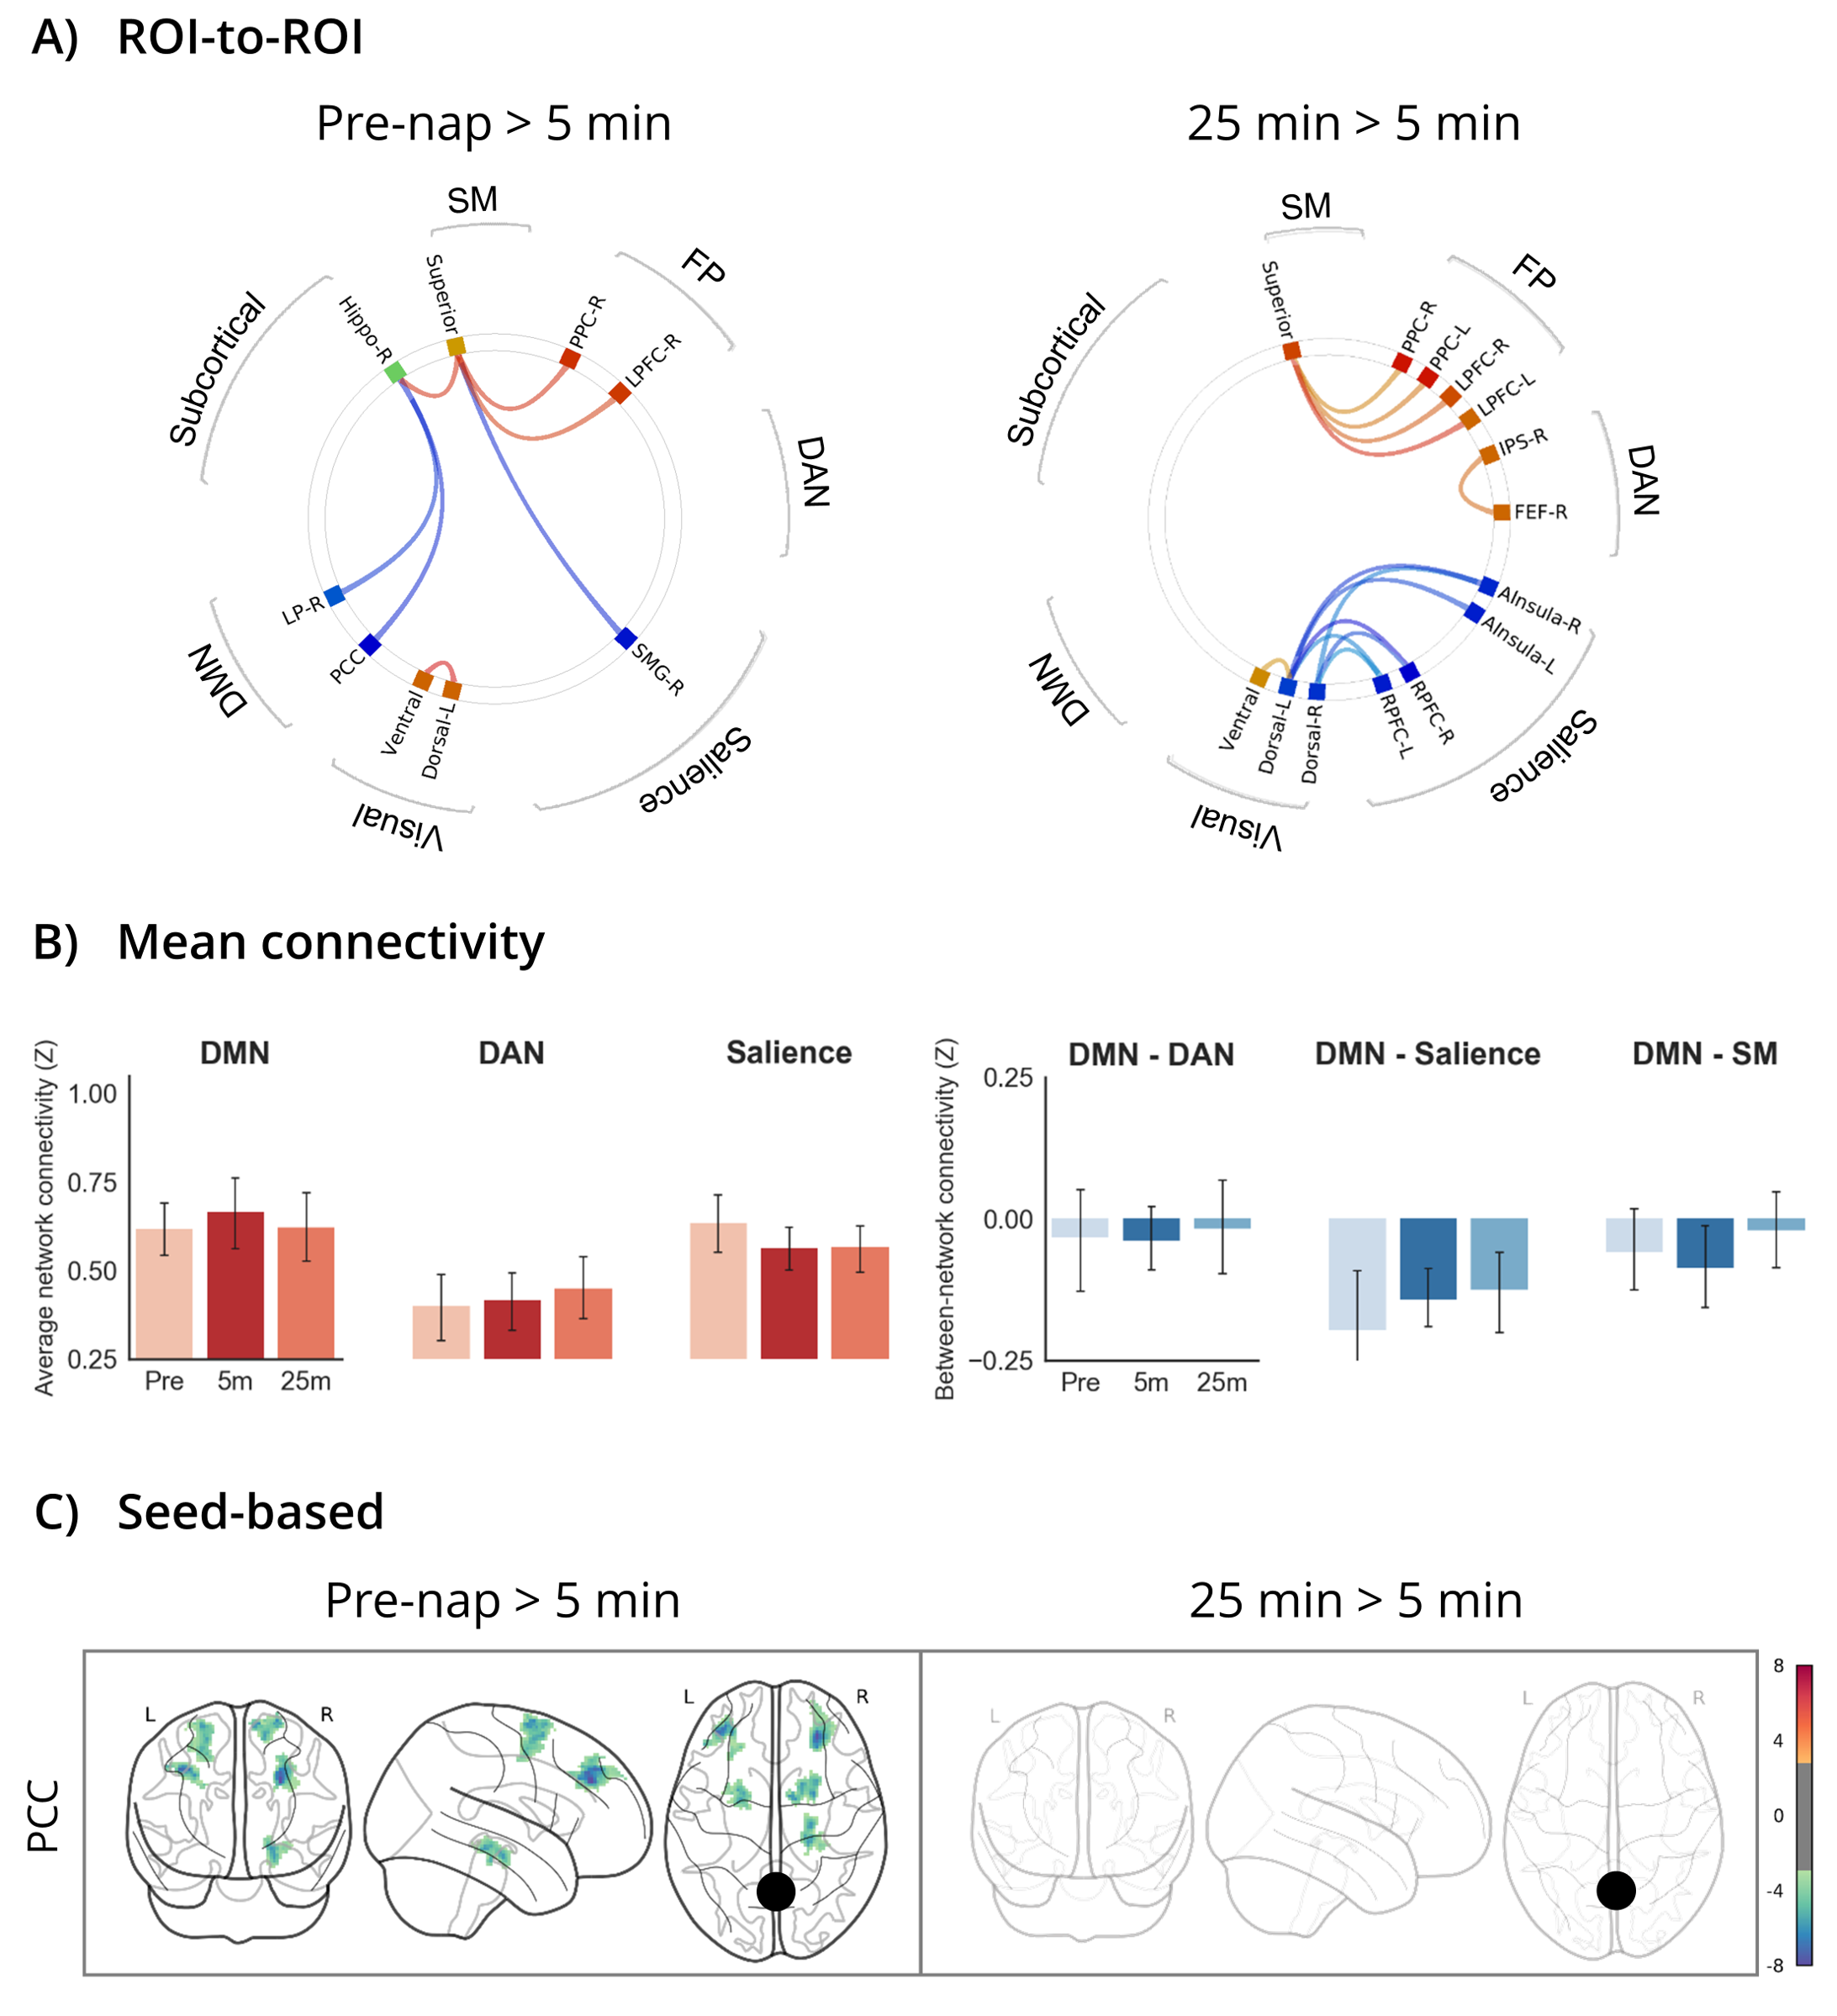
\includegraphics[width=\textwidth]{Fig/Results/Inertia/Inertia/Fig4_N2.png}
	\caption*{\textbf{Fig 4. Functional connectivity disruption after awakening from N2 sleep (n=14)}. (A) ROI-to-ROI results for the two contrasts (left, Pre-nap minus 5 min p-a; right, 25 min p-a minus 5 min p-a). Connections indicate regions with significantly increased (blue lines) or decreased (red lines) pairwise connectivity at 5 min p-a compared to the pre-nap and 25 min p-a scans, respectively (two-sided paired t-test, p<.05 FDR-corrected). (B) Mean pairwise connectivity within (left, red bars) and between (right, blue bars) networks. (C) Seed-based connectivity results for the two contrasts (left, Pre-nap minus 5 min p-a; right, 25 min p-a minus 5 min p-a). Seed region is the posterior cingulate cortex (PCC), one core region of the DMN which demonstrates notable disruption during NREM sleep (center of mass in MNI coordinates: 1, -61, 38). Statistical parametric maps are reported using an uncorrected two-sided cluster-defining voxel-wise height threshold of p<.01 and a whole-brain FWE-corrected extent threshold of p<.05. Yellow-red colors indicate increased connectivity at pre-nap and/or 25 min p-a compared to the 5 min p-a scan. Green-blue colors indicate increased connectivity at 5 min p-a compared to the two other scans.}
\end{figure}

\subsubsection*{Comparison of the functional connectivity alterations following N2 and N3 sleep awakenings}
To further investigate the relationship between functional connectivity alterations and the sleep stage before awakening, we compared the brain connectivity between the N2 and the N3 groups. First, we looked at ROI-to-ROI differences at each resting-state scan (Fig 5A). Interestingly, during the pre-nap scan, the connectivity between the FP network and two regions, the lateral parietal (part of the DMN) and hippocampus, was decreased in the N3 group. At 5 min p-a, participants awakened in N3 sleep had a significantly increased connectivity between the DMN and DAN and between the SM and three networks (DMN, FP, Visual). There was no group difference at 25 min p-a. Next, at 5 min p-a, there was a tendency for a reduced mean DMN connectivity (p=.07) and increased DAN connectivity (p=.08) in the N3 group (Fig 5B, left). Third, the anti-correlations between the DMN and the attentional network and the DMN and the sensori-motor network were significantly decreased in the N3 group (Fig 5B, right, Fig 5D and S3 Table). Finally, we found a significant negative correlation between the mean DMN connectivity at 5 min p-a and the duration of N2/N3 sleep during the nap (Spearman r = -.43, p = .01, Fig 5C). This latter results shows that functional alterations within the DMN are associated with the prior sleep duration.

\begin{figure}[!htbp]
	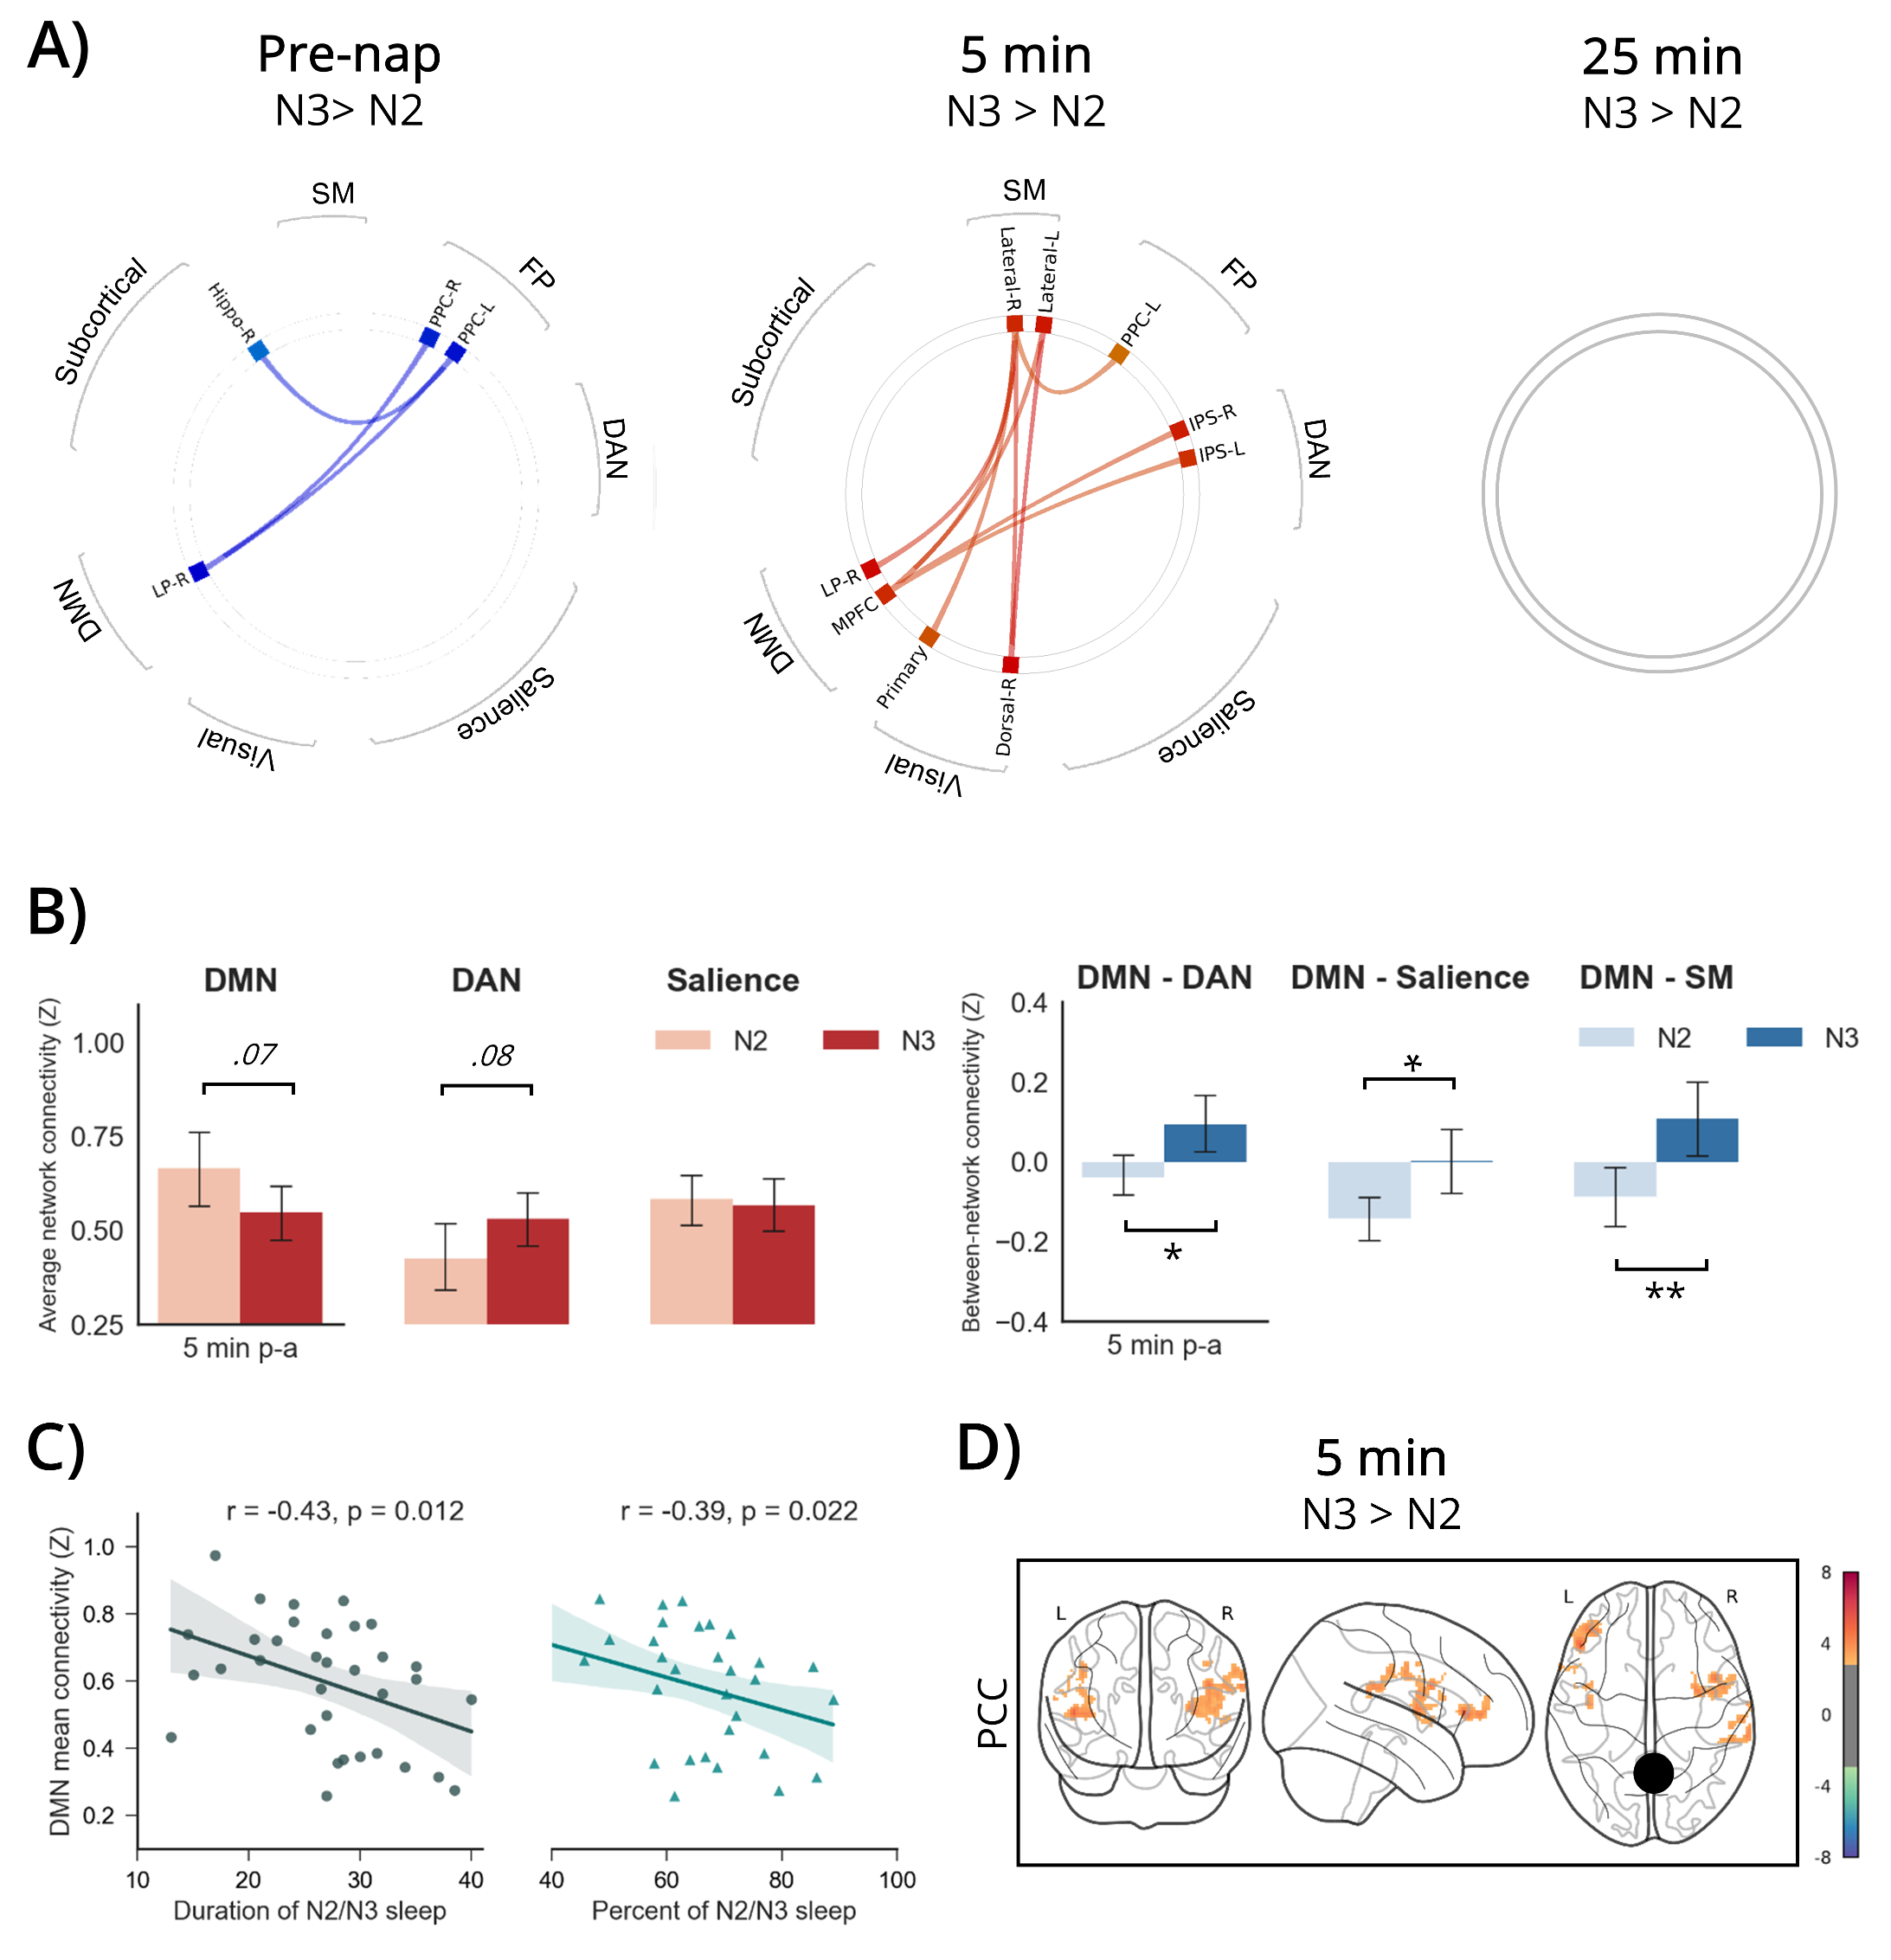
\includegraphics[width=\textwidth]{Fig/Results/Inertia/Inertia/Fig5_N2vsN3.png}
	\caption*{\textbf{Fig 5. Comparison of the functional connectivity after awakening from N3 sleep (n=20) and N2 sleep (n=14).} (A) ROI-to-ROI results at the pre-nap, 5 min and 25 min p-a scans for the contrast N3 minus N2. Blue connections indicate regions with significantly increased (red lines) or decreased (blue lines) connectivity (two-sided t-test, p<.05 FDR-corrected). No difference was found for the 25 min p-a scan. (B) Mean pairwise connectivity within (left, red bars) and between (right, blue bars) networks. Stars denote significant between-group comparisons (t-tests, * p<.05, ** p<.01). (C) Seed-based connectivity results at 5 min p-a for the contrast N3 minus N2. Seed region is the posterior cingulate cortex (PCC), one core region of the DMN which demonstrates notable disruption during NREM sleep (center of mass in MNI coordinates: 1, -61, 38). Statistical parametric maps are reported using an uncorrected two-sided cluster-defining voxel-wise height threshold of p<.01 and a whole-brain FWE-corrected extent threshold of p<.05. Yellow-red colors indicate increased connectivity at pre-nap and/or 25 min p-a compared to the 5 min p-a scan. Green-blue colors indicate increased connectivity at 5 min p-a compared to the two other scans.}
\end{figure}

\FloatBarrier

\subsection*{Discussion}
\label{res:inertia:inertia:discussion}

In a recent review on sleep inertia, \citet{trotti_waking_2016} proposed as first item on a 5-items research agenda that q{if as suggested by PET imaging, resumption of normal waking cognition on awakening requires reorganization of cognitive networks, can other functional neuro-imaging and/or neurophysiologic studies better delineate these necessary network changes?}. The present study aimed at addressing this issue using combined EEG-fMRI, by characterizing the changes in brain networks functional connectivity across the first half hour following awakening from NREM N2 and N3 sleep (resting state scans acquired at 3 time points : pre-sleep, 5 and 25 minutes post-awakening). By contrast with previous studies we also measured behavioral performance (DST) and maximized sleep inertia by partially sleep-depriving the subjects on the night before the experiment, and awakening them after a sustained period of N2 and/or N3 sleep when possible.

\subsubsection*{Performance impairments at awakening}
Using the DST we managed to evidence a decrement in performance after awakening even though the measure was made about 9 minutes after awakening (duration of the resting state scan = 6 min + the average delay between awakening and the scan onset = 3 ± 2 min). We indeed chose to favor the estimation of functional connectivity over the estimation of performance at awakening. For this reason behavioral effects were most probably underestimated in our study.

We found no significant decrement in performance at 5 min p-a compared to pre-sleep. This may be due to the delay between awakening and the first DST and/or to the fact that participants were tired before the nap due to their short night sleep. The total number of responses however was reduced, regardless of the awakening sleep stage and without any significant change in the number of mistakes, at 5 minutes p-a compared to 25 minutes p-a. This observation confirms that sleep inertia effects are conspicuous after a short daytime nap, comprising or not N3 sleep, and is consistent with the generally held view that speed is more impaired than accuracy at awakening \citep{tassi_sleep_2000, trotti_waking_2016}. The relatively smaller decrement in performances observed in the present study compared to previous studies that have used the DST immediately after awakening \citep{dinges_assessing_1985, evans_recovery_1975, stampi_ultrashort_1990} may be accounted for by the delay between the awakening and the task. Our results may therefore suggest that the behavioral aspects of sleep inertia evolve rapidly after awakening and/or are compensated by the beneficial effect of sleep on cognitive performance \citep{faraut_napping:_2016}.

Interestingly we found significantly more mistakes in the N2 group than in the N3 group at 5 min p-a. This finding comes against the idea that the deeper the sleep prior awakening, the worse the performance upon awakening. One explanation could be that the beneficial effect of deep sleep may exceed the detrimental effect of sleep inertia, especially after the above-mentioned 9 min delay between awakening and the first post-sleep DST. Second, this effect may be task-specific. Indeed, the functional connectivity disruptions observed at 5 min p-a from N2 and N3 sleep certainly impact different tasks differently. To our knowledge, no previous studies reported DST performance separately for N2 and N3 sleep. According to our results, the functional connectivity disruptions observed at 5 min p-a from N2 impacts more the performance at the DST than the functional connectivity disruptions observed at 5 min p-a from N3 sleep. The impact on performance may have been reversed if we had used a different task.

\subsubsection*{Functional connectivity alterations after awakening from N3 sleep}
Awakening from N3 sleep was associated with robust and global alterations in the brain connectivity. The most significant finding was the decreased anti-correlation between networks normally anti-correlated during resting wakefulness, such as the task-negative (DMN) on the one hand and the task-positive (DAN, salience) networks on the other hand. This disruption of anti-correlation between task-positive and task-negative networks has been observed in a large palette of states including general anesthesia \citep{boveroux_breakdown_2010}, sleep deprivation \citep{de_havas_sleep_2012, samann_increased_2010, wang_spontaneous_2016} and most importantly during NREM sleep \citep{larson-prior_modulation_2011, samann_development_2011}. This suggests that the functional connectivity during the first minutes following awakening from N3 sleep is marked by an intrusion of sleep specific connectivity into the wakefulness state. Another key finding was that as compared to 5 min p-a, the functional connectivity at 25 min p-a was partially restored between the DMN and DAN and between the thalamus and the frontoparietal network. This change in the dynamic of thalamo-cortical connectivity corroborates previous EEG studies that showed a progressive dissipation of slow wave activity during sleep inertia \citep{ogilvie_falling_1992, ferrara_electroencephalographic_2006, marzano_recalling_2011, gorgoni_eeg_2015}. Finally, using seed-based analyses, we were able to evidence a decreased connectivity between the PCC and the inferior / middle temporal gyrus at 5 min p-a compared to pre-sleep. The middle temporal gyrus has been recently described as part of a DMN subcomponent involved in memory, constructive mental simulations, and according to the author’s postulate, dreaming \citep{christoff_mind-wandering_2016}. It is noteworthy that we observed a reduced connectivity of this region after awakening from N3 sleep which is well known to lead to less dream reports than any other sleep stages \citep{nielsen_review_2000, ruby_experimental_2011}.

\subsubsection*{Functional connectivity alterations after awakening from N2 sleep}
Participants awakened in N2 sleep exhibited little alterations regarding the DMN connectivity and anti-correlations using ROI-to-ROI analysis. One notable exception is the increased connectivity between the DMN and hippocampus at 5 min p-a compared to pre-sleep, which has been reported to predicts subjective sleepiness and worsened working-memory performance under conditions of sleep loss (see \citealp{krause_sleep-deprived_2017}). This and the relative decrease of connectivity in the FP network observed in both ROI-to-ROI and seed-based analysis, could therefore be good candidates to explain the increased percent of mistakes in the N2 group at 5 min p-a compared to the N3 group. Apart from this, we have found at 5 min p-a compared to both pre-sleep and 25 min p-a a strong decrease in the connectivity between the SM and FP networks as well as an increased connectivity between the visual and salience networks. A suboptimal functional connection between the somato-motor network and the executive network may explain the decreased sensori-motor performances (e.g. grip strength, steadiness and coordination) after awakening from N2 sleep reported in several behavioral studies. Similarly the reduced functional connection between the visual and the salience network may be the reason for the deficits in visuo-perceptual tasks at awakening (see \citealp{tassi_sleep_2000}). Finally, at 5 min p-a compared to pre-sleep, seed-based analysis revealed a large increase in the connectivity between the PCC and the parahippocampal gyrus, a region involved in memory retrieval. Such a functional modification may participate in the well-known variability in dream recall between sleep stages \citep{nielsen_review_2000, ruby_experimental_2011}.

\subsubsection*{Link between functional alterations and prior sleep depth / duration}
Several conclusions may be drawn in the light of the above. Awakenings from N2 and N3 sleep were both associated with alterations in functional connectivity. Some of these alterations overlapped and some did not. Regarding the overlap, in both sleep stages we have found strong alterations in the SM network at 5 min p-a. This disruption of SM connectivity was previously reported in two previous studies \citep{wu_variations_2012, tsai_local_2014} and appears to be the physiological signature of the motor impairments and clumsiness classically reported during sleep inertia. Most importantly, there were also several discrepancies in the alterations following N2 or N3 sleep awakening. N3 sleep was characterized by a more robust loss of functional segregation between several networks. Notably, we found large reductions in the anti-correlation between the DMN and task-positive networks (FP, DAN, SM, Salience) as well as an increased connectivity between sensory networks (visual and FP). One key finding is the negative significant correlation between the average DMN mean connectivity and the duration (and percentage) of N2 and N3 sleep during the nap. This result and the previous ones suggest that alterations in the DMN functional connectivity upon awakening are directly linked to the prior sleep duration and depth at least in the first sleep cycle. From a phenomenological standpoint, the intense disruption of the DMN connectivity after awakening from N3 sleep may account for internally-oriented cognitive impairments such as feeling of disorientation, desire to return to sleep and rapid vanishing of short-term memory content (i.e. dreams) frequently observed after awakening from this sleep stage. By contrast, disrupted anti-correlations between the DMN and attentional networks, in addition with reduced FP connectivity, may explain the hypovigilance and reduced cognitive performances which have been consistently reported during sleep inertia. On a more practical level, our findings provide experimental evidences in favor of the general public health advice to take short naps (< 20-30 min) in order to avoid entering N3 sleep, which may suppress the cognitive advantage of taking a nap.

\subsubsection*{Limitations}
Due to the partial sleep deprivation, the functional connectivity during the pre-sleep scan was probably altered as compared to rested wakefulness after a full night of sleep \citep{samann_increased_2010, de_havas_sleep_2012, yeo_functional_2015, kaufmann_brain_2015, tushaus_resisting_2017}. It follows that our results most probably underestimate the functional connectivity disruption associated with sleep inertia. Finally, it is also possible that the MRI scan noise may have had a positive alerting effect on vigilance and therefore reduced the severity of sleep inertia. However, only one study has so far investigated the effect of a pink noise at 75 dB on sleep inertia. The authors reported inconclusive results on whether noise improved or worsened sleep inertia effects after a nap \citep{tassi_effects_1992}.

\subsubsection*{Conclusion}
The present combined EEG-fMRI study provides for the first time a measure of both brain functional connectivity and behavioral performance at 5 and 25 minutes post awakening from N2 and N3 NREM sleep. By splitting participants who were awakened in N2 and N3 sleep, and thanks to a large number of participants (n=55), we were able to provide an exhaustive overview of the functional connectivity alterations following awakening from these two sleep stages. Our results support the hypothesis of \citet{balkin_process_2002} and show that the functional connectivity is altered at awakening from both N2 and N3 sleep, but in a much severe way after an awakening from N3 sleep. Importantly, awakening from N3 sleep induced a severe disruption of the functional connectivity in the default mode network which was not the case for awakening from N2 sleep. In addition, awakenings from N3 sleep were associated with a robust loss of brain functional networks segregation, which severity was correlated with prior sleep duration. Our result provide, as whished by \citet{trotti_waking_2016} in her recent review, the q{which an how} functional brain networks are altered at awakening and show that sleep inertia is the result of an intrusion of sleep specific features in the functional connectivity of the awake brain.

\paragraph{Acknowledgments}
The authors would like to thank Basak Turker, Morgane Hamon, Franck Lamberton and Danielle Ibarrola for substantial help in data collection and analysis, as well as Jamila Lagha for her help in administrative work.

\paragraph{Author contribution}
R.V and P.R designed the study, acquired the data and wrote the paper. D.M helped in data analysis. A.N participated to the design and provided access to his sleep unit to conduct the sleep deprivation.

\newpage

\subsection*{Supplementary materials}
\label{res:inertia:inertia:supp}
\vspace*{1cm}

\begin{figure}[!htbp]
	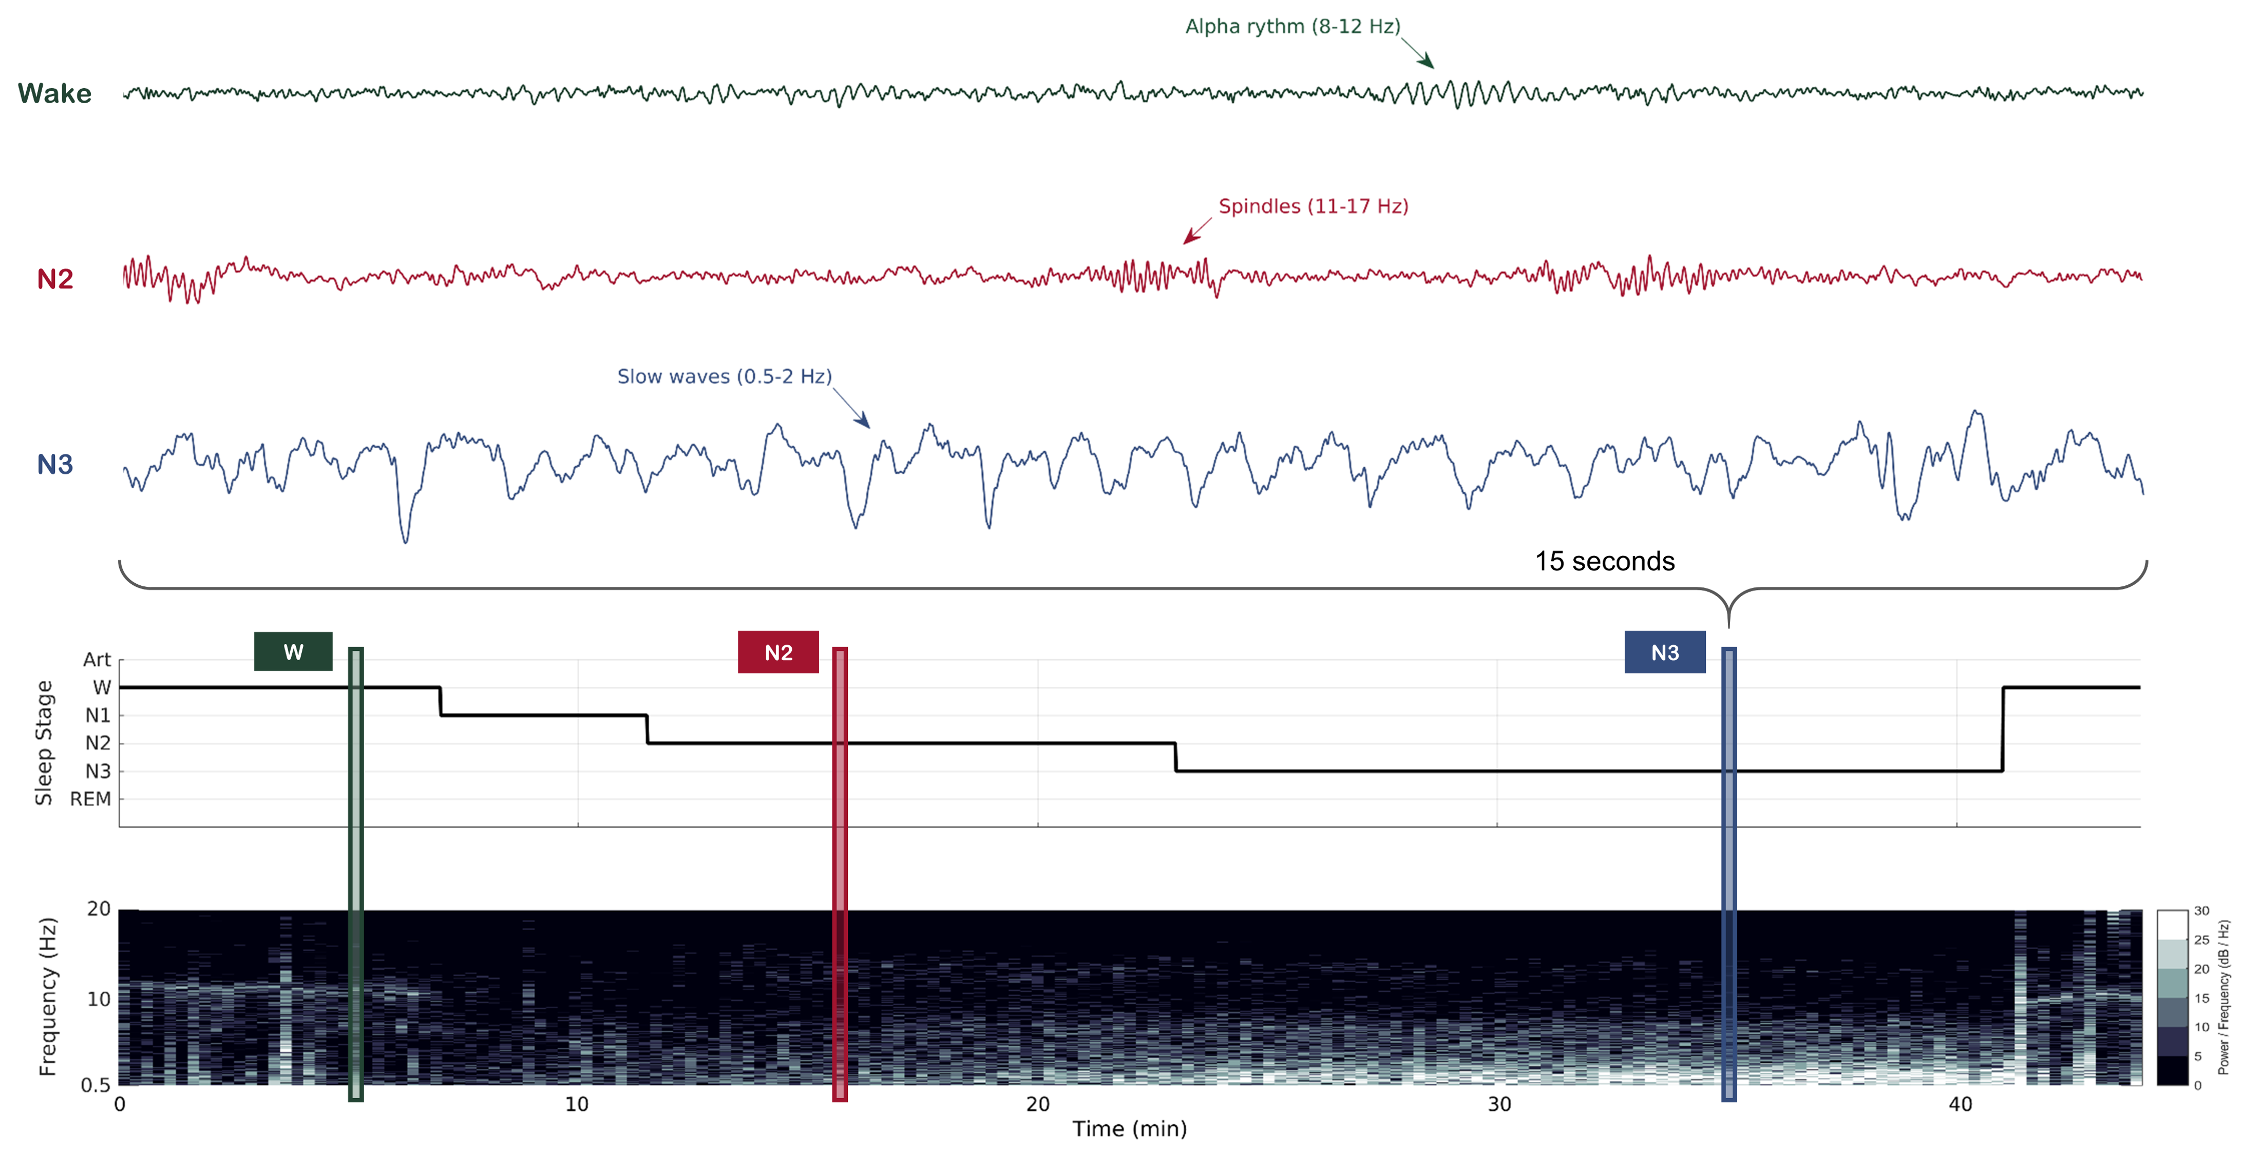
\includegraphics[width=\textwidth]{Fig/Results/Inertia/Inertia/S1_Scoring.png}
	\caption*{\textbf{S1 Fig. Hypnogram and EEG data (Cz) acquired during the nap slot in one subject.} Top. 15-seconds frames of wakefulness, N2 and N3 sleep. Middle. Hypnogram showing vigilance states as function of time during the nap slot. Bottom. Spectrogram showing the normalized power in the 0.5 – 20 Hz range for each 15-seconds frames (lighter colors indicate higher power).}
\end{figure}

\begin{figure}[!htbp]
	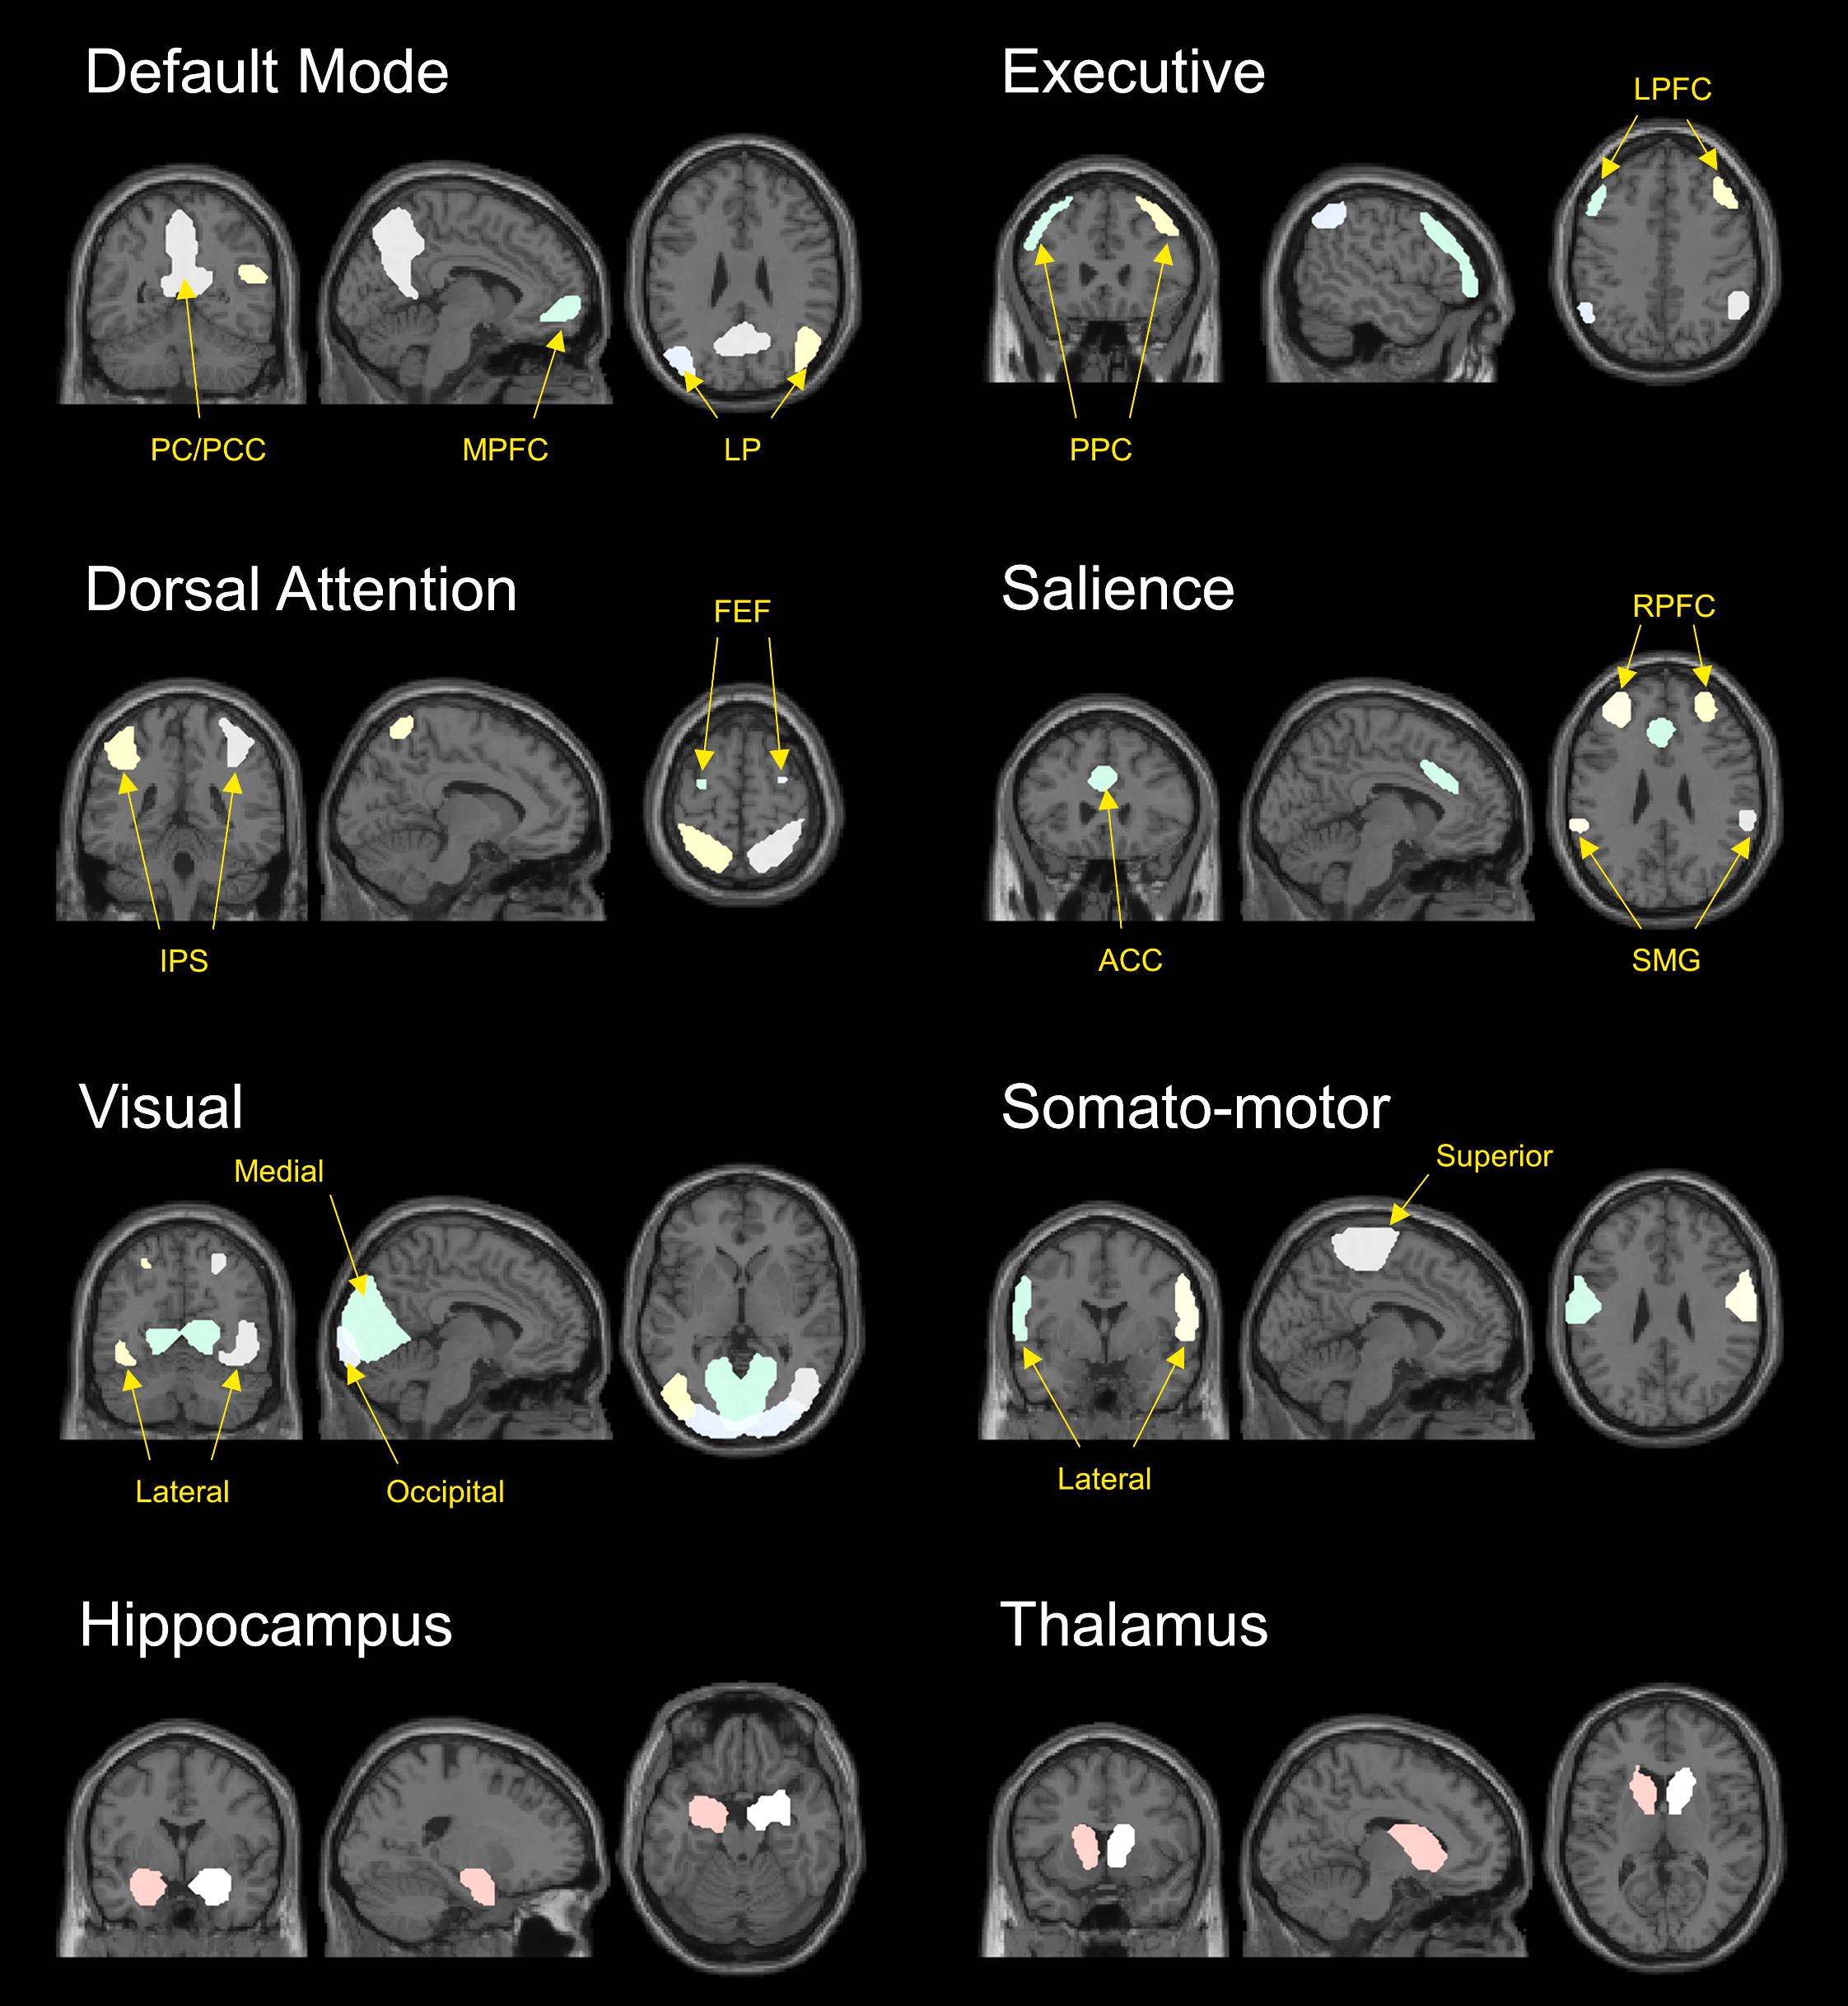
\includegraphics[width=\textwidth]{Fig/Results/Inertia/Inertia/S2_Networks.png}
	\caption*{\textbf{S2 Fig. Networks and regions included in the connectivity analysis.} Abbreviations: PCC/PC, Posterior Cingulate Cortex / Precuneous – MPFC, Medial Prefrontal Cortex – LP, Lateral Parietal – FEF, Frontal Eye Fields – IPS, Intraparietal Sulcus – PPC, Posterior Parietal Cortex – LPFC, Lateral Prefrontal Cortex – ACC, Anterior Cingulate Cortex – RPFC, Rostral Prefrontal Cortex – SMG, Supra-Marginal Gyrus. Note that the salience network also includes the anterior insula (not visible).}
\end{figure}

\FloatBarrier

\begin{table}[htb]
    \caption*{\textbf{S1 Table. Seed-based functional connectivity results for the N3 group (n=20)}. Seed region is the posterior cingulate cortex (PCC, center of mass in MNI coordinates = 1, -61, 38). Statistical analyses were performed using a cluster-defining voxel-wise height threshold of p<.01 (uncorrected, two-sided) and a whole-brain family-wise error (FWE) corrected extent threshold of p<.05 to show brain areas either positively or negatively correlated with the seed region. PG, precentral gyrus - SMG, supramarginal gyrus – ITG, inferior temporal gyrus – SPL, superior parietal lobule – SFG, superior frontal gyrus – N.S, not significant.}
    \resizebox{\textwidth}{!}{%
    \begin{tabularx}{\textwidth}{lXXllllX}
    \toprule
             &              &                    	& \multicolumn{3}{c}{MNI coordinates} 	&         	   &              \\
    Contrast                & Region       			& Brodmann area & X   & Y   & Z   		& T value 	   & Cluster size \\ \midrule
    Pre-sleep > 5 min       & PG L 					& BA44          & -42 & 4   & 26  		& -6.45        & 2980         \\
                            & PG R 					& BA6           & 22  & -14 & 58  		& -6.36        & 1462         \\
                            & SMG L              	& BA40          & -34 & -44 & 34  		& -5.05        & 922          \\
                            & ITG L              	& BA20          & -48 & -6  & -36 		& 6.89         & 742          \\
                            & SPL R              	& BA2           & 40  & -38 & 52  		& -5.10        & 390          \\
                            & PG R 					& BA4           & 8   & -26 & 60  		& -4.14        & 295          \\
                            & SFG R              	& BA6           & 10  & 4   & 66  		& -5.51        & 277          \\
    Pre-sleep > 25 min      & N.S 					& -             & -   & -   & -   		& -            & -            \\
    25 min > 5 min          & PG L 					& BA44          & -42 & 4   & 24  		& -6.68        & 1595         \\
                            & SMG L              	& BA40          & -52 & -46 & 44  		& -5.56        & 879          \\ \bottomrule
    \end{tabularx}%
    }
\end{table}

\begin{table}[htbp]
    \caption*{\textbf{S2 Table. Seed-based functional connectivity results for the N2 group (n=14).} Seed region is the posterior cingulate cortex (PCC, center of mass in MNI coordinates = 1, -61, 38). Statistical analyses were performed using a cluster-defining voxel-wise height threshold of p<.01 (uncorrected, two-sided) and a whole-brain family-wise error (FWE) corrected extent threshold of p<.05. DLPFC, dorsolateral prefrontal cortex – PHG, parahippocampal gyrus – SFG, superior frontal gyrus - N.S, not significant.}
    \begin{tabularx}{\textwidth}{lXXllllX}
    \toprule
    &                       &                       & \multicolumn{3}{c}{MNI coordinates}                &              &               \\
    Contrast                & Region          		& Brodmann area & X          & Y         & Z         & T value 		& Cluster size  \\ \midrule
    Pre-sleep > 5 min       & DLPFC R               & BA9/46        & 28         & 40        & 32        & -5.89        & 464           \\
                            & SFG L                 & BA6           & -22        & -2        & 68        & -6.10        & 351           \\
                            & SFG R                 & BA6           & 26         & 2         & 72        & -6.20        & 271           \\
                            & PHG. R    			& BA34          & 22         & -30       & -12       & -8.40        & 258           \\
                            & DLPFC R               & BA9/46        & -38        & 42        & 40        & -7.01        & 254           \\
    Pre-sleep > 25 min      & N.S    				& -             & -          & -         & -         & -            & -             \\
    25 min > 5 min          & N.S    				& -             & -          & -         & -         & -            & -             \\ \bottomrule
    \end{tabularx}%
\end{table}

\begin{table}[htbp]
    \caption*{\textbf{S3 Table. Seed-based functional connectivity results for the group comparison (N3 (n=20) minus N2 (n=14)).} Seed-based functional connectivity results for the group comparison (N3 (n=20) minus N2 (n=14)). Seed region is the posterior cingulate cortex (PCC, center of mass in MNI coordinates = 1, -61, 38). Statistical analyses were performed using a cluster-defining voxel-wise height threshold of p<.01 (uncorrected, two-sided) and a whole-brain family-wise error (FWE) corrected extent threshold of p<.05 to show brain areas either positively or negatively correlated with the seed region. PG, precentral gyrus - IFG, inferior frontal gyrus – SMG, supramarginal gyrus - N.S, not significant.}
    \begin{tabularx}{\textwidth}{lXXllllX}
    \toprule
    &         &                 & \multicolumn{3}{c}{MNI coordinates}                 &              &              \\
    Scan      & Region    		& Brodmann area & X          & Y          & Z         & T value 		& Cluster size \\ \midrule
    Pre-sleep & N.S 			& -             & -          & -          & -         & -            & -            \\
    5 min     & PG R 			& BA44          & 46         & 8          & 26        & 4.63         & 595          \\
              & IFG L           & BA45          & -48        & 32         & 6         & 5.08         & 314          \\
              & PG L 			& BA4           & -42        & -10        & 36        & 4.90         & 264          \\
              & SMG R           & BA40          & 68         & -32        & 26        & 4.46         & 253          \\
    25 min    & N.S & -         & -          & -          & -         & -            & -            \\ \toprule
    \end{tabularx}%
\end{table}
 % Article Sleep inertia
\cleardoublepage
\section{Sleep inertia in high and low dream recallers}
\label{res:inertia:drf}

\bigskip

\textbf{{\large Brain functional connectivity upon awakening from sleep predicts between-subject differences in dream recall frequency}}

\hfill \emph{In preparation}

\bigskip

Raphael Vallat\textsuperscript{1} (PhD candidate), Alain Nicolas\textsuperscript{1,2} (M.D, PhD), Perrine Ruby\textsuperscript{1} (PhD)

\textsuperscript{1} Lyon Neuroscience Research Center, Brain Dynamics and Cognition team, INSERM UMRS 1028, CNRS UMR 5292, Université Claude Bernard Lyon 1, Université de Lyon, Lyon, France

\textsuperscript{2} Unité Michel Jouvet, Centre Hospitalier Le Vinatier, 95 boulevard Pinel, Lyon, France

\subsection*{Summary}
\label{res:inertia:drf:summary}

Dreaming is a fascinating and universal experience that remains still poorly understood. Perhaps one of its most intriguing aspect relates to why some people recall up to several dreams per day while some hardly ever recall one. Previous results suggest that memory performance during wake could not explain such inter-individual differences in dream recall but that the brain transitional state during sleep inertia immediately following awakening could . To test this hypothesis we designed a combined EEG-fMRI study. We aimed at investigating the brain functional connectivity of high dream recallers (HR, n=27) and low dream recallers (LR, n=27) in the minutes following awakening from a 45 min mid-afternoon nap. Resting-state scans were acquired before the nap, 5 min and 25 min after awakening and were each paired with a mental calculation task. Between-group contrasts of the functional connectivity at 5 min post-awakening revealed a pattern of enhanced connectivity in HR within the default mode network and regions involved in memory retrieval (i.e. medial prefrontal cortex, precuneus, left medial temporal lobe, left dorsolateral prefrontal cortex). These findings are discussed regarding the idea of a neurophysiological trait difference between HR and LR .


\paragraph{Keywords}
Dream recall, sleep inertia, awakening, EEG-fMRI, functional connectivity, default mode network

\subsection*{Introduction}
\label{res:inertia:drf:intro}

Dreaming is a universal and fascinating experience which happens most probably every night when we plunge into sleep. However, several aspects of dreaming are still poorly understood, among which is the large inter-individuals difference in dream recall frequency (DRF). Previous results demonstrated that intra-sleep wakefulness is one explaining factor of DRF variability \citep{eichenlaub_brain_2014, vallat_increased_2017}. However this factor does not explain everything since controlled awakenings in the lab still result in drastically more frequent dream recall in high dream recallers (HR) than in low dream recallers (LR) whatever the sleep stage \citep{goodenough_comparison_1959, eichenlaub_resting_2014, eichenlaub_brain_2014}.

Sleep inertia, the transient period following awakening and associated with impaired performances \citep{tassi_sleep_2000, trotti_waking_2016}, could be the missing link. Awakenings would enable the encoding of the dream into long term memory when the transition between sleep and wakefulness spare the short term memory of the dream \citep{koulack_dream_1976}. The hypothesis is thus that, compared to HR, LR would show more cognitive impairments and functional connectivity disturbances caused by sleep inertia in the first minutes following awakening from sleep. This hypothesis is supported by previous results which have shown functional brain differences between HR and LR using EEG \citep{eichenlaub_brain_2014} and PET \citep{eichenlaub_resting_2014}. As compared to LR, HR notably showed an increased regional cerebral blood flow (rCBF) in the medial prefrontal cortex (MPFC) and temporo-parietal junction (TPJ).

The proper functioning of these regions, known to be involved in dream production and/or recall (i.e. lesions of one or both of these regions induce a cessation of dream reports; \citealp{solms_neuropsychology_1997, solms_dreaming_2000}) could thus explain the successful retrieval of dream content upon awakening. Specifically, we postulate that the strength of the functional connectivity in the network comprising these two regions, namely the default mode network (DMN), is required to recall dreams at awakening. The DMN is a set of functionally coupled brain areas \citep{raichle_default_2001, legrand_what_2009, sestieri_episodic_2011} that are highly activated during mental imagery and episodic memory retrieval, and whose functional connectivity is diminished during sleep \citep{horovitz_decoupling_2009, larson-prior_modulation_2011, samann_development_2011}. Several authors have postulated that the DMN might be the brain network underlying the dreaming experience \citep{domhoff_neural_2011, christoff_mind-wandering_2016}.

The present study aims therefore at testing the hypothesis of a differential brain functioning of HR and LR specifically during the period following awakening from sleep. This hypothesis has surprisingly never been experimentally tested before, despite several studies mentioning the brain and cognitive functioning immediately upon awakening as a potential explaining factor of DRF variability \citep{schredl_factors_2003, conduit_poor_2004}. The period following awakening from sleep is a distinct and transient state that is measurably different from wakefulness since it is characterized by impaired performance, hypovigilance and sleepiness. We therefore hypothesized that sleep inertia and its cerebral correlates may account for the inter-individual differences in DRF. In other words we expected more impaired cognitive performances and functional connectivity at awakening in LR than in HR.

Several studies are consistent with this hypothesis. First, sleep inertia is higher following sleep deprivation or awakening from N3 sleep, which are both factors associated with a lower rate of dream recall \citep{nielsen_review_2000, de_gennaro_recovery_2010}. Second, \citet{conduit_poor_2004} found that memory abilities after awakening from N2 sleep were lower than after awakening from REM sleep, and that these impairments were significantly correlated with reported dream recall frequency (i.e. better memory performances and better dream recall after awakening from REM sleep).

To test our hypotheses, we designed a combined EEG-fMRI study. We aimed at investigating the brain functional connectivity in the minutes following awakening from a 45 minutes mid-afternoon nap in HR vs LR. Resting-state scans were acquired before the nap, 5 min and 25 min after awakening to investigate the dynamics of brain functional reorganization during the first half hour following awakening, and each scan was associated with a mental calculation task to measure the cognitive impairments of sleep inertia. We predicted that HR would show (1) more dream recall following awakening from sleep (2) a higher functional connectivity within the DMN and between regions involved in memory retrieval (3) less cognitive performance impairments, suggesting a faster recovery of normal cognitive functioning upon awakening.

\subsection*{Methods}
\label{res:inertia:drf:methods}

\subsubsection*{Participants}
Behavioral and neurophysiological data were acquired from 55 healthy subjects (28 males, mean age = 22.55, standard deviation = 2.41, range = 19–29). The subjects were informed of the study through an announcement sent to the mailing list of Lyon University, which briefly described the study and included a link to a questionnaire concerning sleep and dream habits. Subjects were selected if they reported and subsequently confirmed during a phone interview: (1) having a high or low DRF (DRF superior to 5 dream recalls per week and inferior to 2 dream recalls per month respectively) (2) having a regular sleep-wake schedule, no difficulty to fall asleep, being occasional or frequent nappers and having preferentially already done an MRI brain scan in the past few years. Importantly, the subjects were unaware that DRF was the main criterion for inclusion in the study. Among the 55 participants, 28 of them were high dream recallers (HR; mean DRF = 6.6 ± 0.7 dream reports per week) and 27 were low dream recallers (LR; mean DRF = 0.2 ± 0.1 dream report per week). Apart from the DRF (p < .001), the two groups did not differ in age, habitual sleep duration or education level (see Table 1 of section \ref{res:dmn-crea:results}). They had no history of neurological and psychiatric disorders, and had no sleep disturbances. They provided written informed consent according to the Declaration of Helsinki and received monetary compensation for their participation. The study was approved by the local ethics committee (CCPPRB, Centre Leon Berard, Lyon, France).

\subsubsection*{Behavioral tests}
The night before the experiment, the subjects underwent a partial sleep deprivation (they were allowed to sleep between 5 am and 8 am; see Procedure). Between 9 pm and 11 pm, the subjects were presented with various tests to assess the potential between group differences at the cognitive and personality levels, the results of which will be detailed elsewhere.

In addition, participants trained on the descending subtraction task (DST), which was used to evaluate cognitive performances during the MRI session on the following day, in order to avoid a practice effect over the first trials \citep{dinges_assessing_1985}. The DST has been previously used to evidence performances decrement and normalization in the first 30 min post awakening \citep{evans_recovery_1975, dinges_assessing_1985, stampi_ultrashort_1990}. Subjects were presented with a three-digit number. They were instructed to subtract 9, saying the operation and the result aloud, and then continue by subtracting 8 from the remainder, then 7, and so on until they had to subtract 1. At this point they were to start the cycle of descending subtractions again. They had to do the task for two minutes and were instructed to be as fast and accurate as possible.

\subsubsection*{Procedure}
\emph{Evening and night}. To facilitate sleep in the MRI environment, participants underwent a 3 h partial sleep deprivation on the night before the experiment. Specifically, they arrived in the sleep unit of the hospital Le Vinatier (Lyon, France) at 8 pm. During two hours they performed the previously described personality and cognitive tests, administered by R.V. They were then instructed to stay awake until 5 am (the possible activities were reading, making puzzles and watching movies), at which point they were allowed to sleep for 3 hours until 8 am in a bed in the sleep unit. Energy drinks or physical activity were prohibited during the partial sleep deprivation, and nurses regularly checked that the subject did not fall asleep. The monitoring of body movements through wrist actigraphy (Actigraph, Pensacola, USA) during the whole night made it possible to check a posteriori that the subject did not fall asleep before 5 am. In the morning, participants were offered breakfast and a shower and then occupied themselves (reading or internet) under the experimenters’ supervision until the MRI session.

\emph{Day}. The MRI procedure is shown in Fig \ref{fig:intro:problematics-fmri-paradigm}. After lunch at 11.30 am, participants were conducted to the neuroimaging center (CERMEP). During the first half hour, experimenters installed on the participant’s head a MRI compatible EEG cap (EASYCAP®). Participants were then installed in the MRI scanner at about 1.20 pm (1.17 pm ± 13 min). They read a 5 min cartoon during the calibration of the eye-tracking camera, and then performed the descending subtraction task (DST) for 2 minutes. The first resting-state scan was then acquired, with the instructions to remain awake and look at a central fixation cross on the screen. At the end of the scan, participants were informed that they could sleep (at 1.39 pm ± 14 min in average) during the next 45 min. At the end of the nap slot, participants were awakened, if they were sleeping, by calling their first name and the 2nd resting state scan was acquired. At the end of the scan, the 2nd DST was performed. During the following 10 minutes, subjects were asked about their dream(s) and sleep in the scanner and about the cartoon. Then the 3rd resting state scan and DST were performed (about 25 min after awakening). Finally, an 8-min T1 anatomical scan was acquired.

\subsubsection*{Data collection}
\paragraph{EEG and eye movement recordings}
Polysomnography data was recorded using a 15 channels MR-compatible cap designed for sleep studies i.e. with a layout designed according to American Academy of Sleep Medicine Guidelines 2007 (EasyCap, Brain Products GmbH, Gilching, Germany). It comprised 9 EEG electrodes placed according to the international standard 10/20 system (O1, O2, C3, C4, F3, F4, M1, M2, Cz, FCz was used as reference and AFz as ground), 2 EOG electrodes, 3 EMG electrodes, and an electrocardiogram electrode placed on the back of the participant. The sampling rate was 5000 Hz and an analog band-pass filter was set to 0.01 – 250 Hz.  To score sleep online during the fMRI session, a real-time pulse-artefact correction was performed using the BrainVision Recorder (Version 1.2) and BrainVision RecView (Version 1.4) softwares (Brain Products).

To ensure that participants were not closing their eyes during the resting state scans, eye movements were monitored during the experiment using an EyeLink 1000 fMRI eye tracking system (SR Research Ontario, Canada). Eye position was calibrated at the beginning of the experiment and monitored throughout.

\paragraph{MRI acquisition}
MRI scans were obtained from a MAGNETOM Prisma 3.0 T scanner (Siemens Healthcare, Erlangen, Germany) at the Primage neuroimaging platform (CERMEP). Structural MRI were acquired with a T1-weighted (0.9-mm isotropic resolution) MPRAGE sequence and functional MRI data with a T2*-weighted 2D gradient echo planar imaging sequence (EPI) with 180 volumes (TR/TE: 2000/ 25 ms; flip angle: 80°; voxel size: 2.68 × 2.68 × 3 mm; slices: 40, duration: 6 minutes). Functional and anatomical scans were performed using a 20-channel head coil. The coil was foam-padded to improve subject comfort and restrict head motion.

\subsubsection*{Data analysis}
\paragraph{EEG}
Artifacts related to gradient switching and cardiac pulse (cardio-ballistic artifact) were removed using standard routines available in BrainVision Analyzer version 2.0 software (Brain Products). Polysomnographic data were downsampled to 1000 Hz and band-pass filtered between 0.5 and 25 Hz. Offline sleep stage scoring was performed using EEG epochs of 30 seconds following standard AASM rules \citep{iber_aasm_2007} visualized using SLEEP software \citep{combrisson_sleep:_2017}.

\paragraph{fMRI}
Preprocessing and quality check were performed using standard routine in SPM12 software (Wellcome Department of Imaging Neuroscience). Preprocessing included functional realignment, slice-time correction, coregistration to structural scan, spatial normalization and spatial smoothing using a 6 mm full-width at half-maximum isotropic Gaussian kernel filter. Individual T1 images were segmented into gray matter, white matter and cerebrospinal fluid tissue maps. Functional and structural images were then normalized to MNI152 space (Montreal Neurological Institute). Functional images underwent artifact and motion regression in the ART toolbox using the following criteria to define outliers: global signal intensity changes greater than 9 standard deviations and movement exceeding 2 mm. SPM motions parameters and outliers were subsequently included as covariates in connectivity analyses.

Connectivity analysis were performed using the CONN toolbox version 17f. First, we performed a denoising step including a regression of the 6 motion correction parameters and their corresponding first-order temporal derivatives, as well as a component-based strategy (aCompCor, \citealp{behzadi_component_2007}) to identify and remove physiological confounds that are unlikely to be related to neural activity. The resulting BOLD time series were band-pass filtered (0.008 – 0.09 Hz) to further reduce noise and increase sensitivity \citep{weissenbacher_correlations_2009}. We then performed seed-to-voxel analysis using a seed in the medial prefrontal cortex (MPFC; center of mass in MNI coordinates: 1, 55, -3), one core region of the DMN which is critically involved in dream recall \citep{solms_neuropsychology_1997, eichenlaub_brain_2014}.

\paragraph{Statistics}
For the DST, between-group comparisons were achieved using a mixed two-way repeated measures ANOVA with a group factor (two levels: HR and LR) and a time factor (within subject factor with three levels: Pre-sleep, 5 min p-a, 25 min p-a). Post hoc analyses (t-tests) were used in case of significance. Seed-based connectivity analysis were performed using a cluster-defining voxel-wise height threshold of p<.01 (uncorrected, two-sided) and a whole-brain family-wise error (FWE) corrected extent threshold of p<.05.

\subsection*{Results}
\label{res:inertia:drf:results}

\subsubsection*{Sleep parameters}
As expected and due to the inherent discomfort of the MRI environment, 11 out of 55 participants were not able to reach N2 sleep during the 45 min nap slot. One subject out of the 44 remaining was discarded because of a technical failure during data acquisition, leading thus to a total of 43 participants included in the final analysis (21 HR, 22 LR). Means of the main sleep parameters in the two groups are presented in Table 1. Importantly, there was no significant group difference for any of the sleep parameters considered or in the latency between the awakening and the two post-awakening resting-state scans.

\begin{table}[!htbp]
    \caption*{\textbf{Table 1. Mean sleep parameters of the HR (n=21) and LR (n=22) groups.} TST = Total Sleep Time, SE = Sleep Efficiency, Wake (W), N1, N2 and N3 = Total duration of each sleep stage in minutes. LAS1 = latency (min) between the awakening and the start of the first post-awakening resting-state scan. LAS2 = latency (min) between the awakening and the start of the second post-awakening resting-state scan. N.S = not significant.}
    \begin{tabularx}{\textwidth}{lXXXXXXXX}
    \toprule
    Group  & TST          & SE (\%)      & W            & N1           & N2           & N3           & LAS1         & LAS2         \\ \midrule
    HR     & 35.6         & 85.7         & 9.3          & 12.9         & 16.8         & 6.3          & 3.4          & 24.3         \\
    SD     & 8.4          & 11.9         & 5.0          & 7.9          & 5.6          & 6.4          & 1.0          & 4.2          \\
    LR     & 36.3         & 83.6         & 11.2         & 11.5         & 18.7         & 6.4          & 4.8          & 23.5         \\
    SD     & 6.3          & 11.7         & 5.2          & 6.9          & 7.3          & 6.0          & 4.0          & 3.6          \\
    T-test & \textit{N.S} & \textit{N.S} & \textit{N.S} & \textit{N.S} & \textit{N.S} & \textit{N.S} & \textit{N.S} & \textit{N.S} \\ \bottomrule
    \end{tabularx}%
\end{table}

\subsubsection*{Behavioral results}
\paragraph{DST}
DST performances are reported in S2 Fig. A two-way ANOVA revealed a significant effect of time in the number of responses (F(2, 41) = 7.44, p = .001) and percentage of correct responses (F(2, 41) = 5.03, p = .009) compared to pre-nap performances.  Specifically, the total number of responses was reduced at 5 min p-a compared to pre-nap and 25 min p-a (p = .003 and p < .001, respectively). There was no main effect of time in the percentage of mistakes, a finding in line with the generally held view that speed is more impaired than accuracy during sleep inertia \citep{trotti_waking_2016}. Most importantly, there was no main effect of group or interaction between group and time for any of the three outcome measures considered. Sleep inertia, as measured by the DST, did not differ between the two groups.

\paragraph{Dream recall}
After awakening from the partial sleep deprivation in the sleep unit, more HR reported dreams than did LR (64\% of HR and 19\% of LR reported a full or a white dream). This was also the case after awakening from the 45 min nap inside the MRI (76\% of HR versus 36\% of LR).

\subsubsection*{Functional connectivity}
The results of functional connectivity contrasts between HR and LR in the three resting-state scans are presented in Fig 1 and Table 2. First, and perhaps most importantly, we found that during the resting-state scan conducted 5 min after awakening from NREM sleep, HR demonstrated an increased functional connectivity between the MPFC and other core regions of the DMN, including the precuneus and temporal fusiform cortex, and between the MPFC and dorsolateral prefrontal cortex (DLPFC). Second, at 25 min post-awakening, seed-based analysis revealed an increased functional connectivity in HR between the MPFC and caudate nucleus. No between-group differences were found during the pre-sleep resting-state scan.

\begin{figure}[!htbp]
	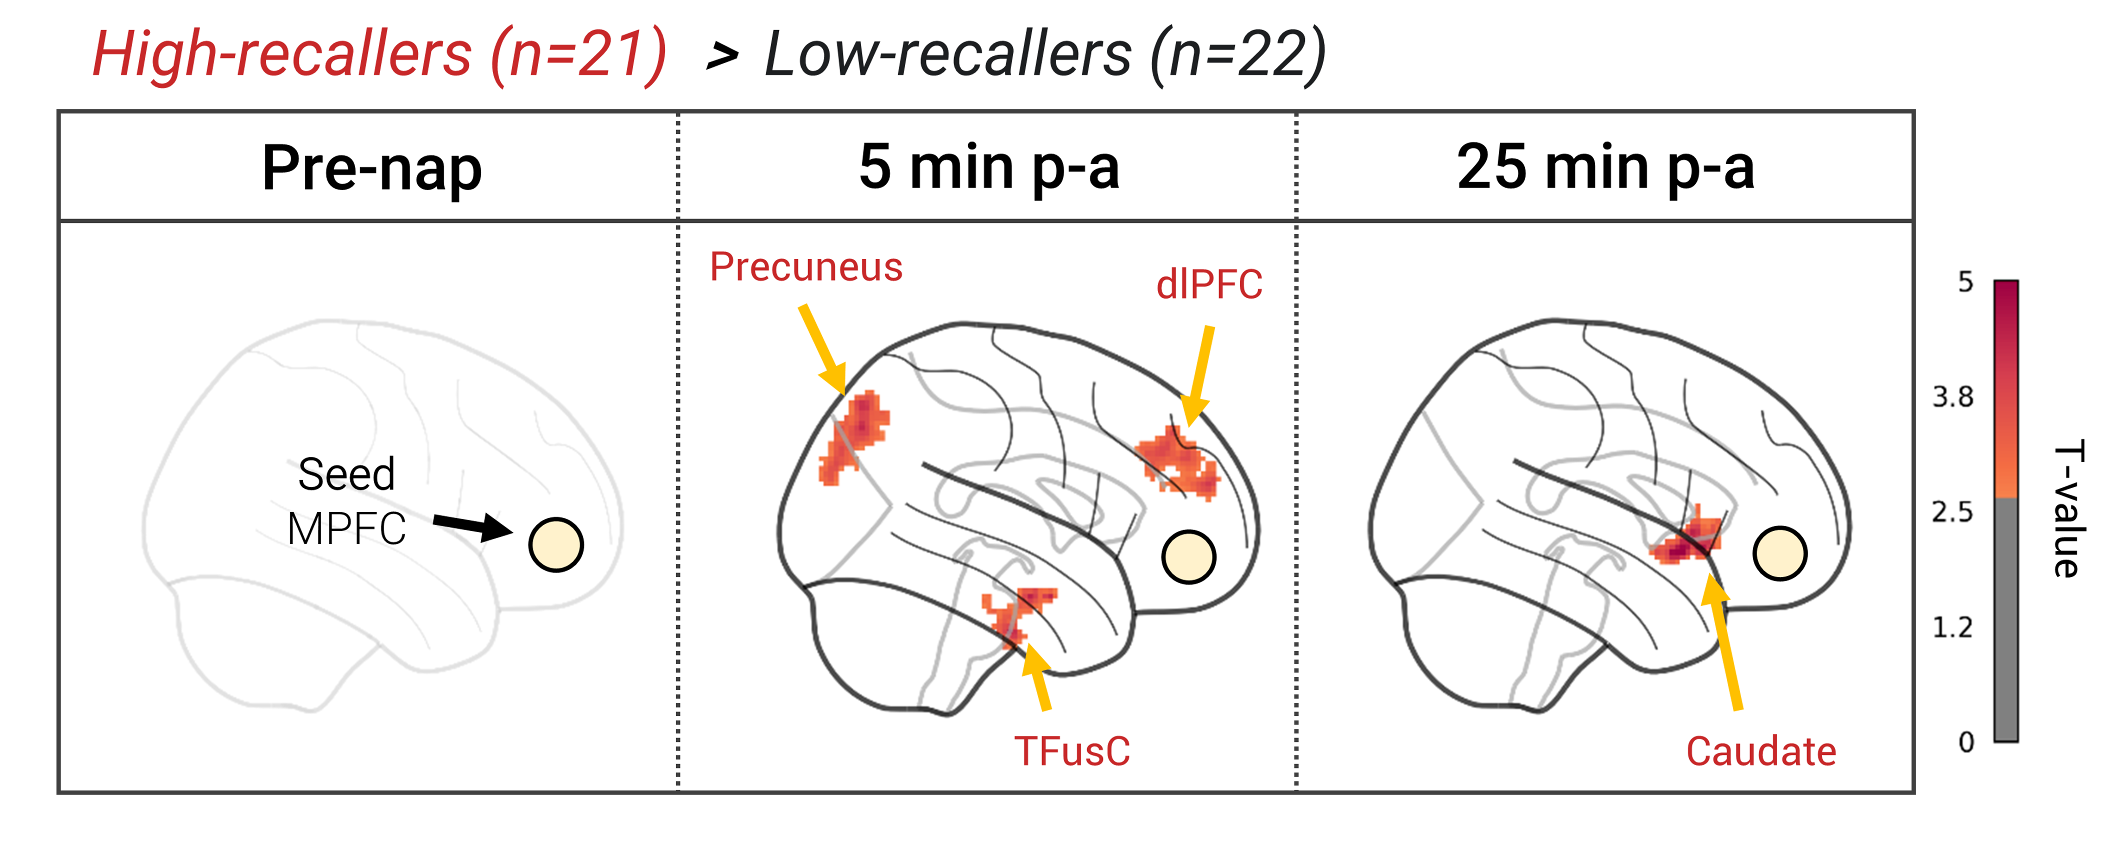
\includegraphics[width=\textwidth]{Fig/Results/Inertia/DRF/Fig1.png}
	\caption*{\textbf{Fig 1. Functional connectivity differences between High-recallers (HR) and Low-recallers (LR) during pre-sleep scan, 5 min post-awakening scan and 25 min post-awakening scan.} Seed-based connectivity results showing foci with higher activation in HR than in LR. Seed region (yellow circle) is the medial prefrontal cortex (MPFC, center of mass in MNI coordinates: 1, 55, -3), a region critically involved in dream recall. Statistical parametric maps are superimposed on a glass brain using an uncorrected two-sided cluster-defining voxel-wise height threshold of p<.01 and a whole-brain FWE-corrected extent threshold of p<.05. MPFC = medial prefrontal cortex, dlPFC = dorsolateral prefrontal cortex, TFusC = temporal fusiform cortex. Faded brain denotes an absence of significant differences between the two groups.}
\end{figure}

\begin{table}[!htbp]
    \caption*{\textbf{Table 2. Seed-based functional connectivity results for the group comparison (HR (n=21) minus LR (n=22))}. Seed region (black circle) is the medial prefrontal cortex (MPFC, center of mass in MNI coordinates = 1, 55, -3). Statistical analyses were performed using a cluster-defining voxel-wise height threshold of p<.01 (uncorrected, two-sided) and a whole-brain family-wise error (FWE) corrected extent threshold of p<.05.}
    \begin{tabularx}{\textwidth}{lXlllXX}
    \toprule
                &              & \multicolumn{3}{l}{MNI coordinates} &              &              \\
    Scan        & Brain region & X          & Y          & Z         & T value      & Cluster size \\ \midrule
    Pre-sleep   & \textit{N.S} & -          & -          & -         & -            & -            \\
    5 min p-a   & Precuneous L & -6         & -76        & 42        & 4.97         & 512          \\
                & DLPFC L      & -34        & 60         & 20        & 4.86         & 356          \\
                & TFC L        & -40        & -18        & -38       & 5.49         & 251          \\
    25 min p-a  & Caudate R    & 14         & 12         & -8        & 6.01         & 277          \\ \bottomrule
    \end{tabularx}
\end{table}

\subsection*{Discussion}
\label{res:inertia:drf:discussion}

This study is the first to compare the brain functional connectivity and cognitive performances of high and low dream recallers in the minutes following awakening from sleep, in an effort to understand the basis for these individual differences in dream recall. The main findings are the followings. First, as expected significantly more HR reported a dream upon awakening than LR. Second, compared to LR, the brain functional connectivity of HR at 5 min post-awakening was significantly increased in several regions that all have in common to be involved in memory processes. Third, the arithmetic performances of both HR and LR were significantly impaired at 5 min post-awakening compared to pre-nap and 25 min post awakening, but no between group differences was observed. The significance of these findings is discussed below.

Between-group contrasts of the functional connectivity at 5 min post-awakening revealed a pattern of enhanced connectivity in HR within the DMN (namely the precuneus, medial prefrontal cortex and left medial temporal lobe) and between the DMN and the left DLPFC. Remarkably, all these regions have been associated with memory processes. In a meta-analysis of the brain areas associated with episodic encoding and retrieval, \citet{spaniol_event-related_2009} reported that the largest clusters associated with retrieval success were located in the precuneus, the anterior prefrontal cortex, the left DLPFC and, to a lesser extent, the middle temporal gyrus. These are almost exactly the same regions found to be more functionally connected in HR than LR during the first minutes following awakening.

Based on these findings, one may conclude that HR were deliberately involved in memory retrieval during the resting-state scans, hence an increase functional connectivity in these specific regions. This hypothesis is however unlikely given that subjects were asked to remember the content of their dreams only during the interval between the 5 min and 25 min post-awakening scans. Moreover, only 5 subjects (4 HR) reported that they were actively trying to recall the content of their dreams during the 5 min post-awakening scan.  Another possible interpretation is that these results reflect neurophysiological trait differences rather than strategy/task differences between HR and LR. This interpretation is supported by previous results showing, in HR, increased brain responses to auditory stimuli during wakefulness and sleep \citep{eichenlaub_brain_2014}, and increased regional cerebral blood flow in the MPFC and TPJ, also during sleep and wakefulness \citep{eichenlaub_resting_2014}. Since it is generally admitted that sleep inertia interferes with memory retrieval on awakening rather than memory consolidation \citep{bonnet_memory_1983, dinges_are_1990, tassi_sleep_2000, conduit_poor_2004}, the findings of the present study support the hypothesis of a differential brain functional organization upon awakening between HR and LR.  Specifically, increased functional connectivity between regions involved in memory retrieval would facilitate dream recall in HR, while decreased connectivity in those same regions would prevent successful dream recall in LR. These results suggest that the difference in DRF between HR and LR is not the result of a differential production of dreams, but rather of a differential recall of dreams upon awakening .

\subsubsection{Limitations}
First, the present study reported the brain functional connectivity of HR and LR following awakening from sleep stages, namely N2 and N3 sleep. It would be interesting to extend these data to N1 sleep and REM sleep. This latter, which has traditionally been viewed as the neural substrate of dreaming, is however very difficult to observe in an fMRI setting, unless applying a severe and specific REM sleep deprivation in the night(s) before \citep{duyn_eeg-fmri_2012}, which is of course not ideal to study functional connectivity given the huge impact of severe sleep deprivation on the brain functional connectome \citep{de_havas_sleep_2012, yeo_functional_2015, krause_sleep-deprived_2017}. Given the higher rate of dream recall following REM sleep than any other sleep stages \citep{nielsen_review_2000, ruby_experimental_2011}, one would expect that the functional connectivity between regions involved in memory retrieval would be higher following awakening from REM sleep than NREM sleep. This would in turn explain the better cognitive and memory performances (i.e. lesser sleep inertia) following REM sleep than NREM sleep \citep{bonnet_memory_1983, koukkou_dreaming:_1983, conduit_poor_2004}.

On another note, we were not able to evidence between-group differences in cognitive performances, measured by the DST, at 5 min post-awakening. There are two possible reasons for this. First, the DST was not performed immediately after awakening but after the 6 min resting-state scans, because we choose to favor the estimation of functional connectivity rather than cognitive performances directly upon awakening. \citet{bonnet_memory_1983} reported that the impairment of cognitive and memory performance upon awakening decreases as a function of time awake. Therefore the delay between awakening and the DST could account for a relatively small decrease in performance compared to pre-nap performances and the absence of group main effect. Second, while the DST has been previously reported to be affected by sleep inertia \citep{dinges_assessing_1985}, it is possible that this arithmetic task do not capture well the brain functioning and dream recall differences between HR and LR, as would have for instance a task more-specifically designed to assess memory retrieval.

\subsubsection{Conclusion}
The present study showed that inter-individual differences in dream recall frequency are associated with a differential brain functional connectivity in the minutes following awakening. Specifically, a higher functional connectivity between regions involved in memory retrieval just after awakening could facilitate in HR the retrieval of pre-awakening experiences and thus promote dream recall. More broadly, these results contribute to the growing body of evidence that trait differences in dream recall are supported by trait neurophysiological correlates. Further work is needed to better delineate the interactions between neurophysiological factors, psychological factors and inter-individual differences in dream recall.

% \paragraph{Acknowledgments}
% The authors would like to thank Basak Turker, Morgane Hamon, Franck Lamberton and Danielle Ibarrola for substantial help in data collection and analysis, as well as Jamila Lagha for her help in administrative work.
%
% \paragraph{Author contribution}
% R.V and P.R designed the study, acquired the data and wrote the paper. A.N participated to the design and provided access to his sleep unit to conduct the sleep deprivation.

\FloatBarrier

\subsection*{Supplementary materials}

S1 Fig is a duplicate of Fig \ref{fig:intro:problematics-fmri-paradigm} of the present thesis.

S1 table is a duplicate of Table 1 Study 3 (section \ref{res:dmn-crea:results}).

\vspace*{1cm}

\begin{figure}[!htbp]
	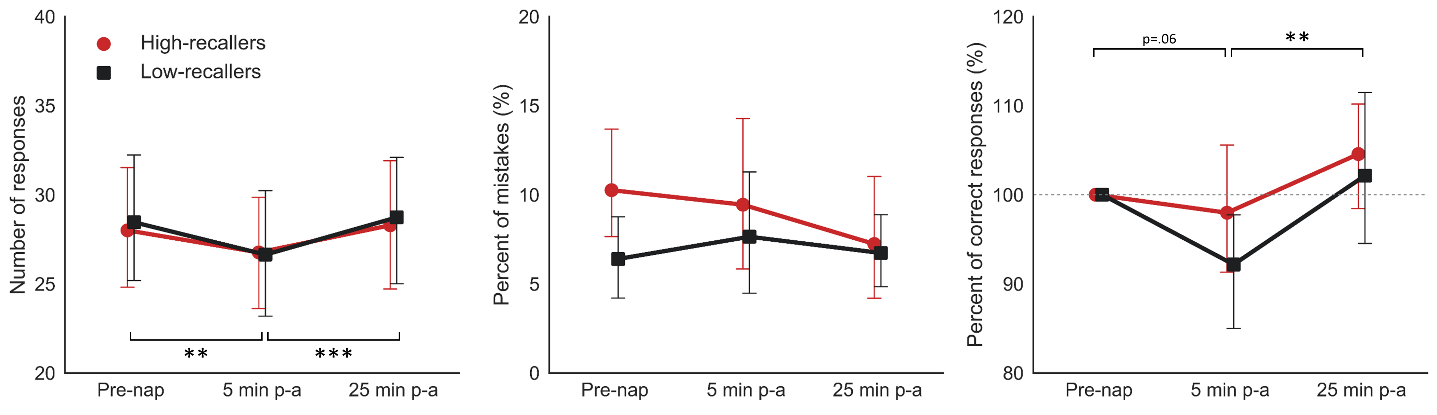
\includegraphics[width=\textwidth]{Fig/Results/Inertia/DRF/S2_Fig.png}
	\caption*{\textbf{S2 Fig. Performances of the Descending Subtraction Task.} Red lines, High-recallers (n=21), black lines, Low-recallers (n=22). (A) Total number of responses (index of speed). (B) Percentage of mistakes (marker of accuracy). (C) Percentage of correct responses relative to pre-nap performances (marker of both speed and accuracy). Error bars represent 95\% confidence intervals. * p<.05, *** p<.001}
\end{figure}
 % Article DRF & Sleep inertia

\cleardoublepage

\chapter{Study 3}
\label{res:dmn-crea}

\textbf{{\large High dream recall frequency is associated with increased creativity and functional connectivity in the default mode network}}

\hfill \emph{In preparation}

\bigskip

Raphael Vallat\textsuperscript{1} (PhD candidate), Alain Nicolas\textsuperscript{1,2} (M.D, PhD), Perrine Ruby\textsuperscript{1} (PhD)

\textsuperscript{1} Lyon Neuroscience Research Center, Brain Dynamics and Cognition team, INSERM UMRS 1028, CNRS UMR 5292, Université Claude Bernard Lyon 1, Université de Lyon, Lyon, France

\textsuperscript{2} Unité Michel Jouvet, Centre Hospitalier Le Vinatier, 95 boulevard Pinel, Lyon, France

\subsection*{Summary}
\label{res:dmn-crea:summary}
Several results suggest that the frequency of dream recall is positively correlated with personality traits such as creativity and openness to experience. These findings are coherent with neuroimaging result showing different neurophysiological profiles in high dream recallers (HR) and low dream recallers (LR).  As compared to LR, a higher regional cerebral blood flow within core regions of the default mode network has been observed in HR during sleep and wakefulness. These observations are consistent with the emerging view that dreaming and mind wandering pertain to the same family of spontaneous mental processes, subserved by the default mode network. To further test this hypothesis, we assessed in HR (n=28) and LR (n=27) the (1) functional connectivity in the default mode network during resting wakefulness using fMRI as well as (2) creative-thinking, personality traits and cognitive abilities. As expected, HR demonstrated a greater DMN connectivity than LR, higher scores of creativity, and no significant difference in cognitive or memory abilities. These results support the forebrain and the DMN hypotheses of dreaming and suggest that increased activity in the DMN promote creative-thinking during both wakefulness and sleep. 

\paragraph{Keywords}
Dream recall, creativity, resting state, functional connectivity, default mode network

\subsection*{Introduction}
\label{res:dmn-crea:intro}
Despite recent advances, the cerebral mechanisms favoring the production or memory of dreams are still poorly understood (see \citealp{ruby_experimental_2011}). While dreaming has long been equated with rapid eye movement (REM), it is now well established that dreaming can also occur in any sleep stages and is therefore not exclusive to a specific functional brain state. Since it is impossible to know for sure when one is actually dreaming while asleep, most empirical investigation of dreaming are therefore based on the study of dream report after awakening the dreamer \citep{schwartz_dreaming:_2005}.

As a consequence, neurophysiological studies on dreaming have either focused on comparing the brain activity in the minutes preceding an awakening associated with the presence or absence of dream recall \citep{esposito_reduced_2004, wittmann_nrem_2004, chellappa_cortical_2011, marzano_recalling_2011, scarpelli_state-_2015, siclari_neural_2017}, or on investigating the cognitive and brain functioning associated with high or low dream recall frequency (DRF; \citealp{eichenlaub_brain_2014, eichenlaub_resting_2014}).

With respect to the second line of research, recent works from our team highlighted several neurophysiological differences between high dream recallers (HR) and low dream recallers (LR), not only during sleep but also during wakefulness \citealp{eichenlaub_brain_2014, eichenlaub_resting_2014, vallat_increased_2017}. For instance, we compared using PET the spontaneous regional cerebral blood flow (rCBF) of HR and LR during sleep and wakefulness, and showed that HR have a higher spontaneous rCBF than LR in the temporo-parietal junction (TPJ) and in the medial prefrontal cortex (MPFC) during REM sleep, N3 sleep and wakefulness \citep{eichenlaub_resting_2014}. We argued that these two regions must play a key role in dream production or recall since lesions of these same areas have been found to be consistently correlated with global or partial cessation of dream reporting (without any concurrent sleep disturbance; see \citealp{solms_neuropsychology_1997}). It is noteworthy that the MPFC and TPJ are part of the default mode network (DMN), a set of functionally-coupled brain regions which are highly activated during internally oriented mental processes and memory retrieval \citep{gusnard_searching_2001, raichle_default_2001}. This network is centered on the MPFC, the posterior cingulate cortex (PCC) and the lateral parietal (LP) areas around the TPJ area.

The finding of a higher spontaneous rCBF within core regions of the DMN in HR compared to LR provides strong evidence supporting the hypothesis of a differential cognitive and brain functioning between high and low frequency dream recallers. This idea was first put forward by \citet{schonbar_differential_1965} who postulated that high dream recall is part of a general life style characterized, inter alia, by creativity, divergent thinking and introspection. Several subsequent works confirmed this hypothesis by showing a substantial correlation between DRF and creativity \citep{fitch_variations_1989, schredl_creativity_1995, schredl_factors_2003}, and DRF and personality traits such as openness to experience \citep{hartmann_boundaries_1989, schredl_dreaming_1996, schredl_dream_2003}. These observations fit remarkably well within the emerging view that dreaming and creative-thinking are both members of a broad family of spontaneous-thought phenomena, which also includes mind-wandering and daydreaming \citep{christoff_mind-wandering_2016}. Several works indicate that dreaming and creativity could be both underpinned by a strong recruitment of the DMN, and especially the prefrontal areas \citep{domhoff_neural_2011, ellamil_evaluative_2012, jung_structure_2013, beaty_creativity_2014, mok_interplay_2014, beaty_default_2015, christoff_mind-wandering_2016}.

The main conclusion to be drawn from these studies is that high dream recall seems to be on one hand related to the spontaneous activity of the DMN, and the other hand related to a general life style involving at least higher creativity. The purpose of the present study is to go a step further by characterizing the intrinsic DMN functional connectivity of HR and LR during resting-state wakefulness, as well as measures of personality, cognitive abilities and creativity. The results highlight a greater DMN connectivity in HR which was concomitant with higher scores of creativity. These results were not associated with further group differences in cognitive or memory abilities.

\subsection*{Methods}
\label{res:dmn-crea:methods}

\subsubsection*{Participants}
Behavioral and neurophysiological data were acquired from 55 healthy subjects (28 males, mean age = 22.55, standard deviation = 2.41, range = 19–29). The subjects were informed of the study through an announcement sent to the mailing list of Lyon University, which briefly described the study and included a link to a questionnaire concerning sleep and dream habits. Subjects were selected if they reported and subsequently confirmed during a phone interview: (1) having a high or low DRF (DRF superior to 5 dream recall per week and inferior to 2 dream recall per month respectively) (2) having a regular sleep-wake schedule, no difficulty to fall asleep, being occasional or frequent nappers and having preferentially already done an MRI brain scan in the past few years. Importantly, the subjects were unaware that DRF was the main criterion for inclusion in the study.

Among the 55 participants, 28 of them were high dream recallers (HR; mean DRF = 6.6 ± 0.6 dream reports per week) and 27 were low dream recallers (LR; mean DRF = 0.2 ± 0.1 dream report per week). Apart from the DRF (p<.0001), the two groups did not differ in age, habitual sleep duration or education level (Table 1). They had no history of neurological and psychiatric disorders, and had no sleep disturbances. The local ethics committee (Centre Leon Bérard, Lyon) approved this study, and subjects provided written, informed consent in conformity with the Declaration of Helsinki. The subjects were paid for their participation.

\subsubsection*{Procedure}
This study is related to a larger combined EEG-fMRI study investigating the differences between high and low dream recallers during the minutes following awakening from a short daytime nap. On this occasion, we acquired three six minutes resting-state scans, located before, 5 min after awakening and 25 min after awakening, respectively. The procedure is detailed as follows. After lunch at 11.30 am, participants were conducted to the neuroimaging center (CERMEP). During the first half hour, experimenters installed on the participant’s head a MRI compatible EEG cap (EASYCAP®). Participants were then installed in the MRI scanner at about 1.20 pm (1.17 pm ± 13 min). The first resting-state scan was then acquired, with the instructions to remain awake and look at a central fixation cross on the screen. At the end of the scan, participants were informed that they could sleep during the next 45 min. At the end of the nap slot, participants were awakened, if they were sleeping, by calling their first name and the 2nd resting state scan was acquired. During the following 10 minutes, subjects were asked about their dream(s) and sleep in the scanner. Then the 3rd resting state scan was performed about 25 min after awakening. Finally, an 8-min T1 anatomical scan was acquired. To facilitate sleep in the MRI environment, participants were allowed to sleep between 5 am and 8 am the night before the experiment. The partial sleep deprivation took place under the constant supervision of nurses in the sleep unit of Le Vinatier Hospital.

\subsubsection*{Data collection and analysis}
\paragraph{MRI acquisition}
MRI scans were obtained from a MAGNETOM Prisma 3.0 T scanner (Siemens Healthcare, Erlangen, Germany) at the Primage neuroimaging platform (CERMEP). Structural MRI were acquired with a T1-weighted (0.9-mm isotropic resolution) MPRAGE sequence and functional MRI data with a T2*-weighted 2D gradient echo planar imaging sequence (EPI) with 180 volumes (TR/TE: 2000/ 25 ms; flip angle: 80°; voxel size: 2.68 × 2.68 × 3 mm; slices: 40, duration: 6 minutes). Functional and anatomical scans were performed using a 20-channel head coil. The coil was foam-padded to improve subject comfort and restrict head motion.

\paragraph{Behavioral tests}
In addition with neurophysiological measures, participants were presented with various tests to assess the potential between group differences at the cognitive and personality levels. These tests were administered by author R.V during the evening prior to the partial sleep deprivation. A detail description follows.

\emph{BFI}. The Big Five Inventory (BFI) is a self-report inventory designed to measure the Big Five dimensions \citep{john_big_1999}, which have been typically labelled as O (Openness to experience), C (Conscientiousness), E (Extraversion), A (Agreeableness), N (Neuroticism). We used the validated French version (BFI-Fr; \citealp{plaisant_validation_2010}), which includes 45 items presenting a collection of statements concerning interpersonal relationships and personality. Each item is scored on a 5-point Likert-type response scale, ranging from 'strongly disagree' (1) to 'strongly agree' (5).

\emph{STAI}. The State-Trait Anxiety Inventory (STAI) is a self-report inventory consisting of 40 items pertaining to anxiety affect \citep{spielberger_manual_1970}. The STAI purports to measure one's conscious awareness at two extremes of anxiety affect, labeled state anxiety (A-state), and trait anxiety (A-trait), respectively. The A-Trait and A-State scales comprise 20 items each, scored on a 4-point Likert-type response scale. Scores range from 20 to 80, with higher scores suggesting greater levels of anxiety.

\emph{PQSI}. The Pittsburgh Sleep Quality Index (PQSI) is a self-rated questionnaire which assesses sleep quality and disturbances over a one-month time interval \citep{buysse_pittsburgh_1989}. It comprises 19 individual items concerning among others subjective sleep quality, sleep latency, sleep duration and daytime dysfunction. Higher scores at the PQSI indicate poorer sleep quality.

\emph{MEM-III}. The MEM-III is the validated French version of the Wechsler Memory Scale (WMS-third edition, WMS-III; \citealp{wechsler_mem-iii:_2001}).  We used a subtest to assess immediate and delayed memory. Participants were read the first story, after which they were instructed to say out loud everything they could remember of this story. The experimenter rated how many items (maximum 25) the participants were able to recall. Twenty five minutes later, the subjects were asked again to recall the stories (delayed memory). Importantly, the subjects were not aware that they would have to recall any of the images at any point after the test. For both immediate and delayed recall, scores were averaged over the two stories and therefore range from 0 to 50, with higher scores reflecting greater memory performances.

\emph{Digit span}. Individual memory abilities were also assessed using a digit span task, which measures the working memory’s number storage capacity. Participants were asked to repeat a heard sequence of numerical digits, the length of which increases at each trial. Digit span was assessed first forwards (maximum score 16) and then backwards (maximum score 14). The digit span index was obtained by averaging the two scores. Higher scores (maximum 30) indicate higher working memory abilities.

\emph{Guildford’s Alternative Uses Task}. The Guildford Uses Task \citep{guildford_alternate_1978} is a creativity test in which participants are asked to list as many possible uses for an everyday object. Participants were shown images of three objects (a pen, a mug, a chair) in a randomized order and subsequently asked to list, during 2 minutes, as many alternative or unusual uses for this object. The fluency index is the total number of responses averaged across the three items. Higher scores indicate higher creativity. Additionally, we computed for each subject and each item the number of rare uses (top 10\% rarest uses, i.e. uses found by 5 or less participants). The rare uses index is the total number of rare uses averaged across the three items. Higher scores indicate higher creativity.

\paragraph{fMRI analysis}
One subject (HR) was excluded from the MRI analysis because of a technical failure during MRI acquisition, leading to a total of 27 HR and 27 LR. As the failure only concerned MRI acquisition, the behavioral and cognitive measures of this participant were still included in the analysis. For the remaining subjects, preprocessing and quality check were performed using standard routine in SPM12 software (Wellcome Department of Imaging Neuroscience). Preprocessing included functional realignment, slice-time correction, coregistration to structural scan, spatial normalization and spatial smoothing using a 6 mm full-width at half-maximum isotropic Gaussian kernel filter. Individual T1 images were segmented into gray matter, white matter and cerebrospinal fluid tissue maps. Functional and structural images were then normalized to MNI152 space (Montreal Neurological Institute). Functional images underwent artifact and motion regression in the Artifact Detection Toolbox using the following criteria to define outliers: global signal intensity changes greater than 9 standard deviations and movement exceeding 2 mm. SPM motions parameters and outliers were subsequently included as covariates in connectivity analyses.

Connectivity analysis were performed on the concatenated resting-state scans (3 scans x 6 minutes = 18 minutes resting-state data) using the CONN toolbox version 17f \citep{whitfield-gabrieli_conn:_2012}. As the aim of this study was to compare the DMN connectivity during resting-state between HR and LR, we selected 4 main regions of interests (ROIs) corresponding to the core nodes of the DMN (see Fig 1A). These include the Posterior Cingulate Cortex (PCC; center of mass in MNI coordinates: 1, -61, 38), the Medial Prefrontal Cortex (MPFC; 1, 55, -3) and bilateral Lateral Parietal cortices (LP; left: -39, -77, 33, right: 47, -67, 29). These regions are implemented within the CONN Toolbox version 17f as part of a parcellation atlas of the main brain networks, obtained by applying an independent component analysis on 467 subjects from the Human Connectome Project.

The connectivity analysis included the following steps: first, we performed a denoising step including a regression of the 6 motion correction parameters and their corresponding first-order temporal derivatives, as well as a component-based strategy (aCompCor, \citealp{behzadi_component_2007}) to identify and remove physiological confounds that are unlikely to be related to neural activity. The resulting BOLD time series were band-pass filtered (0.008 – 0.09 Hz) to further reduce noise and increase sensitivity \citep{weissenbacher_correlations_2009}. Then, Pearson’s correlation coefficients were calculated for each pair-wise connection across the 4 nodes of the DMN, resulting in a single skew-symmetric connectivity matrix with 6 correlation coefficients for each subject. These values were normalized using a Fisher’s r-to-Z transformation and then compared between HR and LR (two-sided t-tests corrected for multiple comparisons using the false discovery rate (FDR, p<.05)). Finally, the mean DMN connectivity (average of all pair-wise correlations) was calculated and compared between groups.

\paragraph{Statistics}
As several studies reported a higher creativity in HR than in LR, between group comparisons of the fluency index and rare uses index were achieved using one-tailed T-test (p<.05). Similarly, as we expected HR to demonstrate a higher DMN functional connectivity than LR, between group statistical comparisons of the mean DMN functional connectivity was achieved using one-tailed T-test. All the other comparisons were achieved using two-sided T-tests.

\subsection*{Results}
\label{res:dmn-crea:results}


\setlength\LTleft{0pt}
\setlength\LTright{0pt}
\renewcommand{\arraystretch}{.9}
\begin{longtable}{@{\extracolsep{\fill}}lllllll@{}} % xlxllxx
    \caption*{\textbf{Table 1. Subject information.} DRF: habitual weekly dream recall frequency (the number of awakenings per week with a dream in mind). Gender: subject’s gender (F, female; M, male). Age: subject’s age (years). Sleep duration: habitual sleep duration during the week (hours). Education: number of years of education. Age, habitual sleep duration and education level were not significantly different between High-recallers and Low-recallers; however, the DRF was significantly larger in High-recallers than in Low-recallers (t-test, ***P<0.0001).} \\
    \toprule
	Group          	& N° & DRF            & Gender & Age  			& Sleep duration	& Education       \\ \midrule
	High recallers 	& 1  & 6              & M      & 19.3 			& 7             	& 0               \\
	               	& 2  & 7              & M      & 23.9 			& 8             	& 3               \\
	               	& 3  & 7              & M      & 22.6 			& 8             	& 4               \\
	               	& 4  & 7              & F      & 21.0 			& 9             	& 3               \\
	               	& 5  & 7              & F      & 24.1 			& 8.3           	& 5               \\
	               	& 6  & 7              & F      & 19.4 			& 7.5           	& 1               \\
	               	& 7  & 5              & F      & 23.7 			& 8.33          	& 4               \\
	               	& 8  & 7              & M      & 23.8 			& 8             	& 3               \\
	               	& 9  & 6              & M      & 27.2 			& 7.5           	& 8               \\
	               	& 10 & 7              & M      & 23.9 			& 8             	& 5               \\
	               	& 11 & 7              & F      & 18.9 			& 9             	& 1               \\
	               	& 12 & 7              & F      & 24.2 			& 8.5           	& 5               \\
	               	& 13 & 6              & M      & 23.0 			& 6             	& 5               \\
	               	& 14 & 6              & F      & 21.1 			& 8.5           	& 3               \\
	               	& 15 & 7              & F      & 20.6 			& 8.5           	& 3               \\
	               	& 16 & 6              & M      & 28.1 			& 7             	& 9               \\
	               	& 17 & 7              & F      & 19.6 			& 8             	& 1               \\
	               	& 18 & 7              & F      & 23.9 			& 7             	& 5               \\
	               	& 19 & 6              & M      & 22.7 			& 9             	& 4               \\
	               	& 20 & 6              & M      & 21.8 			& 9             	& 3               \\
	               	& 21 & 7              & F      & 20.8 			& 8             	& 4               \\
	               	& 22 & 7              & M      & 26.3 			& 7             	& 4               \\
	               	& 23 & 7              & F      & 19.1 			& 8             	& 1               \\
	               	& 24 & 7              & F      & 21.1 			& 7             	& 4               \\
	               	& 25 & 7              & F      & 22.7 			& 6             	& 4               \\
	               	& 26 & 7              & F      & 23.2 			& 9             	& 5               \\
	               	& 27 & 6              & M      & 22.3 			& 8             	& 10              \\
	               	& 28 & 6              & M      & 21.0 			& 7             	& 3               \\
	Low recallers  	& 1  & 0.5            & F      & 25.3 			& 8             	& 4               \\
	               	& 2  & 0.5            & M      & 23.3 			& 8             	& 4               \\
	               	& 3  & 0              & M      & 21.0 			& 6             	& 2               \\
	               	& 4  & 0              & M      & 23.7 			& 9             	& 5               \\
	               	& 5  & 0.3            & M      & 28.2 			& 7.5           	& 7               \\
	               	& 6  & 0.3            & F      & 21.2 			& 9             	& 3               \\
	               	& 7  & 0.25           & M      & 23.2 			& 6.5           	& 5               \\
	               	& 8  & 0              & F      & 25.0 			& 8             	& 6               \\
	               	& 9  & 0.25           & F      & 22.2 			& 8             	& 2               \\
	               	& 10 & 0.1            & F      & 19.2 			& 9.5           	& 1               \\
	               	& 11 & 0.1            & M      & 21.1 			& 8             	& 4               \\
	               	& 12 & 0.3            & F      & 21.6 			& 7             	& 4               \\
	               	& 13 & 0.25           & F      & 19.1 			& 8             	& 1               \\
	               	& 14 & 0.25           & F      & 18.9 			& 8.5           	& 2               \\
	               	& 15 & 0.25           & F      & 22.9 			& 6.5           	& 5               \\
	               	& 16 & 0.25           & M      & 25.0 			& 8             	& 5               \\
	               	& 17 & 0.25           & M      & 21.2 			& 8             	& 3               \\
	               	& 18 & 0.5            & M      & 23.8 			& 7             	& 6               \\
	               	& 19 & 0.1            & M      & 24.0 			& 7             	& 6               \\
	               	& 20 & 0.3            & M      & 29.1 			& 7             	& 4               \\
	               	& 21 & 0.25           & M      & 22.8 			& 8             	& 4               \\
	               	& 22 & 0.25           & F      & 23.3 			& 7             	& 5               \\
	               	& 23 & 0              & F      & 21.0 			& 6             	& 4               \\
	               	& 24 & 0.25           & F      & 21.1 			& 6             	& 3               \\
	               	& 25 & 0.25           & M      & 20.8 			& 8             	& 3               \\
	               	& 26 & 0              & M      & 21.0 			& 8             	& 4               \\
	               	& 27 & 0.25           & M      & 20.0 			& 8            		& 2               \\
	\textbf{Mean HR}&  	 & \textbf{6.6}   &        & \textbf{22.5} 	& \textbf{7.9} 		& \textbf{3.9}    \\
	STD HR         	&    & 0.6            &        & 2.4  			& 0.9          		& 2.3             \\
	\textbf{Mean LR}&    & \textbf{0.2}   &        & \textbf{22.6} 	& \textbf{7.6} 		& 3.9             \\
	STD LR         	&    & 0.1            &        & 2.5  			& 0.9          		& \textbf{1.6}    \\
	T-test         	&    & \textless.0001 &        & 0.89 			& 0.28         		& 0.89            \\ \bottomrule
\end{longtable}

% Revert table spacing to default
\renewcommand{\arraystretch}{1.2}

\subsubsection*{Behavioral tests}
Results of the cognitive and personality tests are reported in Table 2. First, we did not find any significant differences in the memory abilities of HR and LR, as measured by the MEM-III scale and digit span task. Second, there was no significant difference in the PQSI score. Third, there was no difference in the state and trait anxiety levels, as measured by the STAI self-report scale. Fourth, the Big Five personality dimensions were not significantly different between the two groups, however there was a tendency (p=.07) for a higher agreeableness score in HR than in LR, a dimension related to the tendency to be compassionate and cooperative rather than suspicious and antagonistic towards others.

Finally, we observed significant between group differences in creativity scores (Fig 2). HR were found to have a higher fluency index at the Guildford’s alternate uses task. The effect was significant for the pen object (HR = 8.4 ± 2.6, LR = 6.6 ± 2.1, T(53) = 2.86, p = .003) and after averaging for each subject the fluency index of the three objects (HR = 8.2 ± 2.4, LR = 7.2 ± 2.3, T(53) = 1.68, p = .049). Furthermore, they also reported a significantly greater number of rare uses. The effect was significant for the pen (HR = 3.1 ± 1.7, LR = 2.2 ± 1.8, T(53) = 1.88, p = .033), the mug (HR = 3.8 ± 2.5, LR = 2.8 ± 1.8, T(53) = 1.72, p = .045) and after averaging for each subject the rare uses index of the three objects (HR = 3.1 ± 1.6, LR = 2.3 ± 1.5, T(53) = 1.77, p = .042).

\begin{table}[htbp]
    \caption*{\textbf{Table 2. Behavioral results of the cognitive and personality traits (n=55, 28 HR, 27 LR)}. BFI = Big Five Inventory, STAI = State-trait Anxiety Inventory, PQSI = Pittsburgh Sleep Quality Index. All p-values derived from two-sided T-tests.}
    \begin{tabularx}{\textwidth}{lXXll}
    \toprule
	Test                     & High recallers & Low recallers & T     & P-value \\ \midrule
	BFI                      &                &               &       &         \\
	- Openness to experience & 3.8 ± 0.6      & 3.7 ± 0.5     & 0.52  & 0.61    \\
	- Conscientiousness      & 3.3 ± 0.7      & 3.6 ± 0.6     & -1.39 & 0.17    \\
	- Extraversion           & 3.4 ± 0.8      & 3.3 ± 0.7     & 0.54  & 0.59    \\
	- Agreeableness          & 4.0 ± 0.6      & 3.7 ± 0.6     & 1.87  & 0.07    \\
	- Neuroticism            & 2.9 ± 0.8      & 2.5 ± 0.9     & 1.34  & 0.19    \\
	STAI                     &                &               &       &         \\
	- State anxiety          & 33.5 ± 8.9     & 29.9 ± 8.6    & 1.55  & 0.13    \\
	- Trait anxiety          & 39.7 ± 10.6    & 36.9 ± 9.0    & 1.03  & 0.31    \\
	MEM-III                  &                &               &       &         \\
	- Immediate recall       & 29.4 ± 4.9     & 28.9 ± 7.2    & 0.30  & 0.76    \\
	- Delayed recall         & 31.8 ± 5.1     & 31.7 ± 6.9    & 0.05  & 0.96    \\
	PQSI                     & 4.8 ± 2.6      & 4.3 ± 1.9     & 0.78  & 0.44    \\
	Digit span               & 17.6 ± 3.0     & 18.4 ± 3.6    & -0.9  & 0.37    \\ \bottomrule
    \end{tabularx}%
\end{table}

\subsubsection*{Functional connectivity}
The mean DMN functional connectivity was higher in HR than in LR (HR = 0.64 ± 0.14, LR = 0.56 ± 0.16, T(52) = 1.81, p = .038; Fig 1B). The DMN connectivity matrices for each group with pairwise connectivity color coded by strength are presented in Fig 1C. Between group comparisons of the connectivity matrices indicated a greater connectivity between the MPFC and right LP (effect size = 0.16, T(52) = 2.70, p-FDR = .028, p-unc = .009).

\begin{figure}[!htbp]
	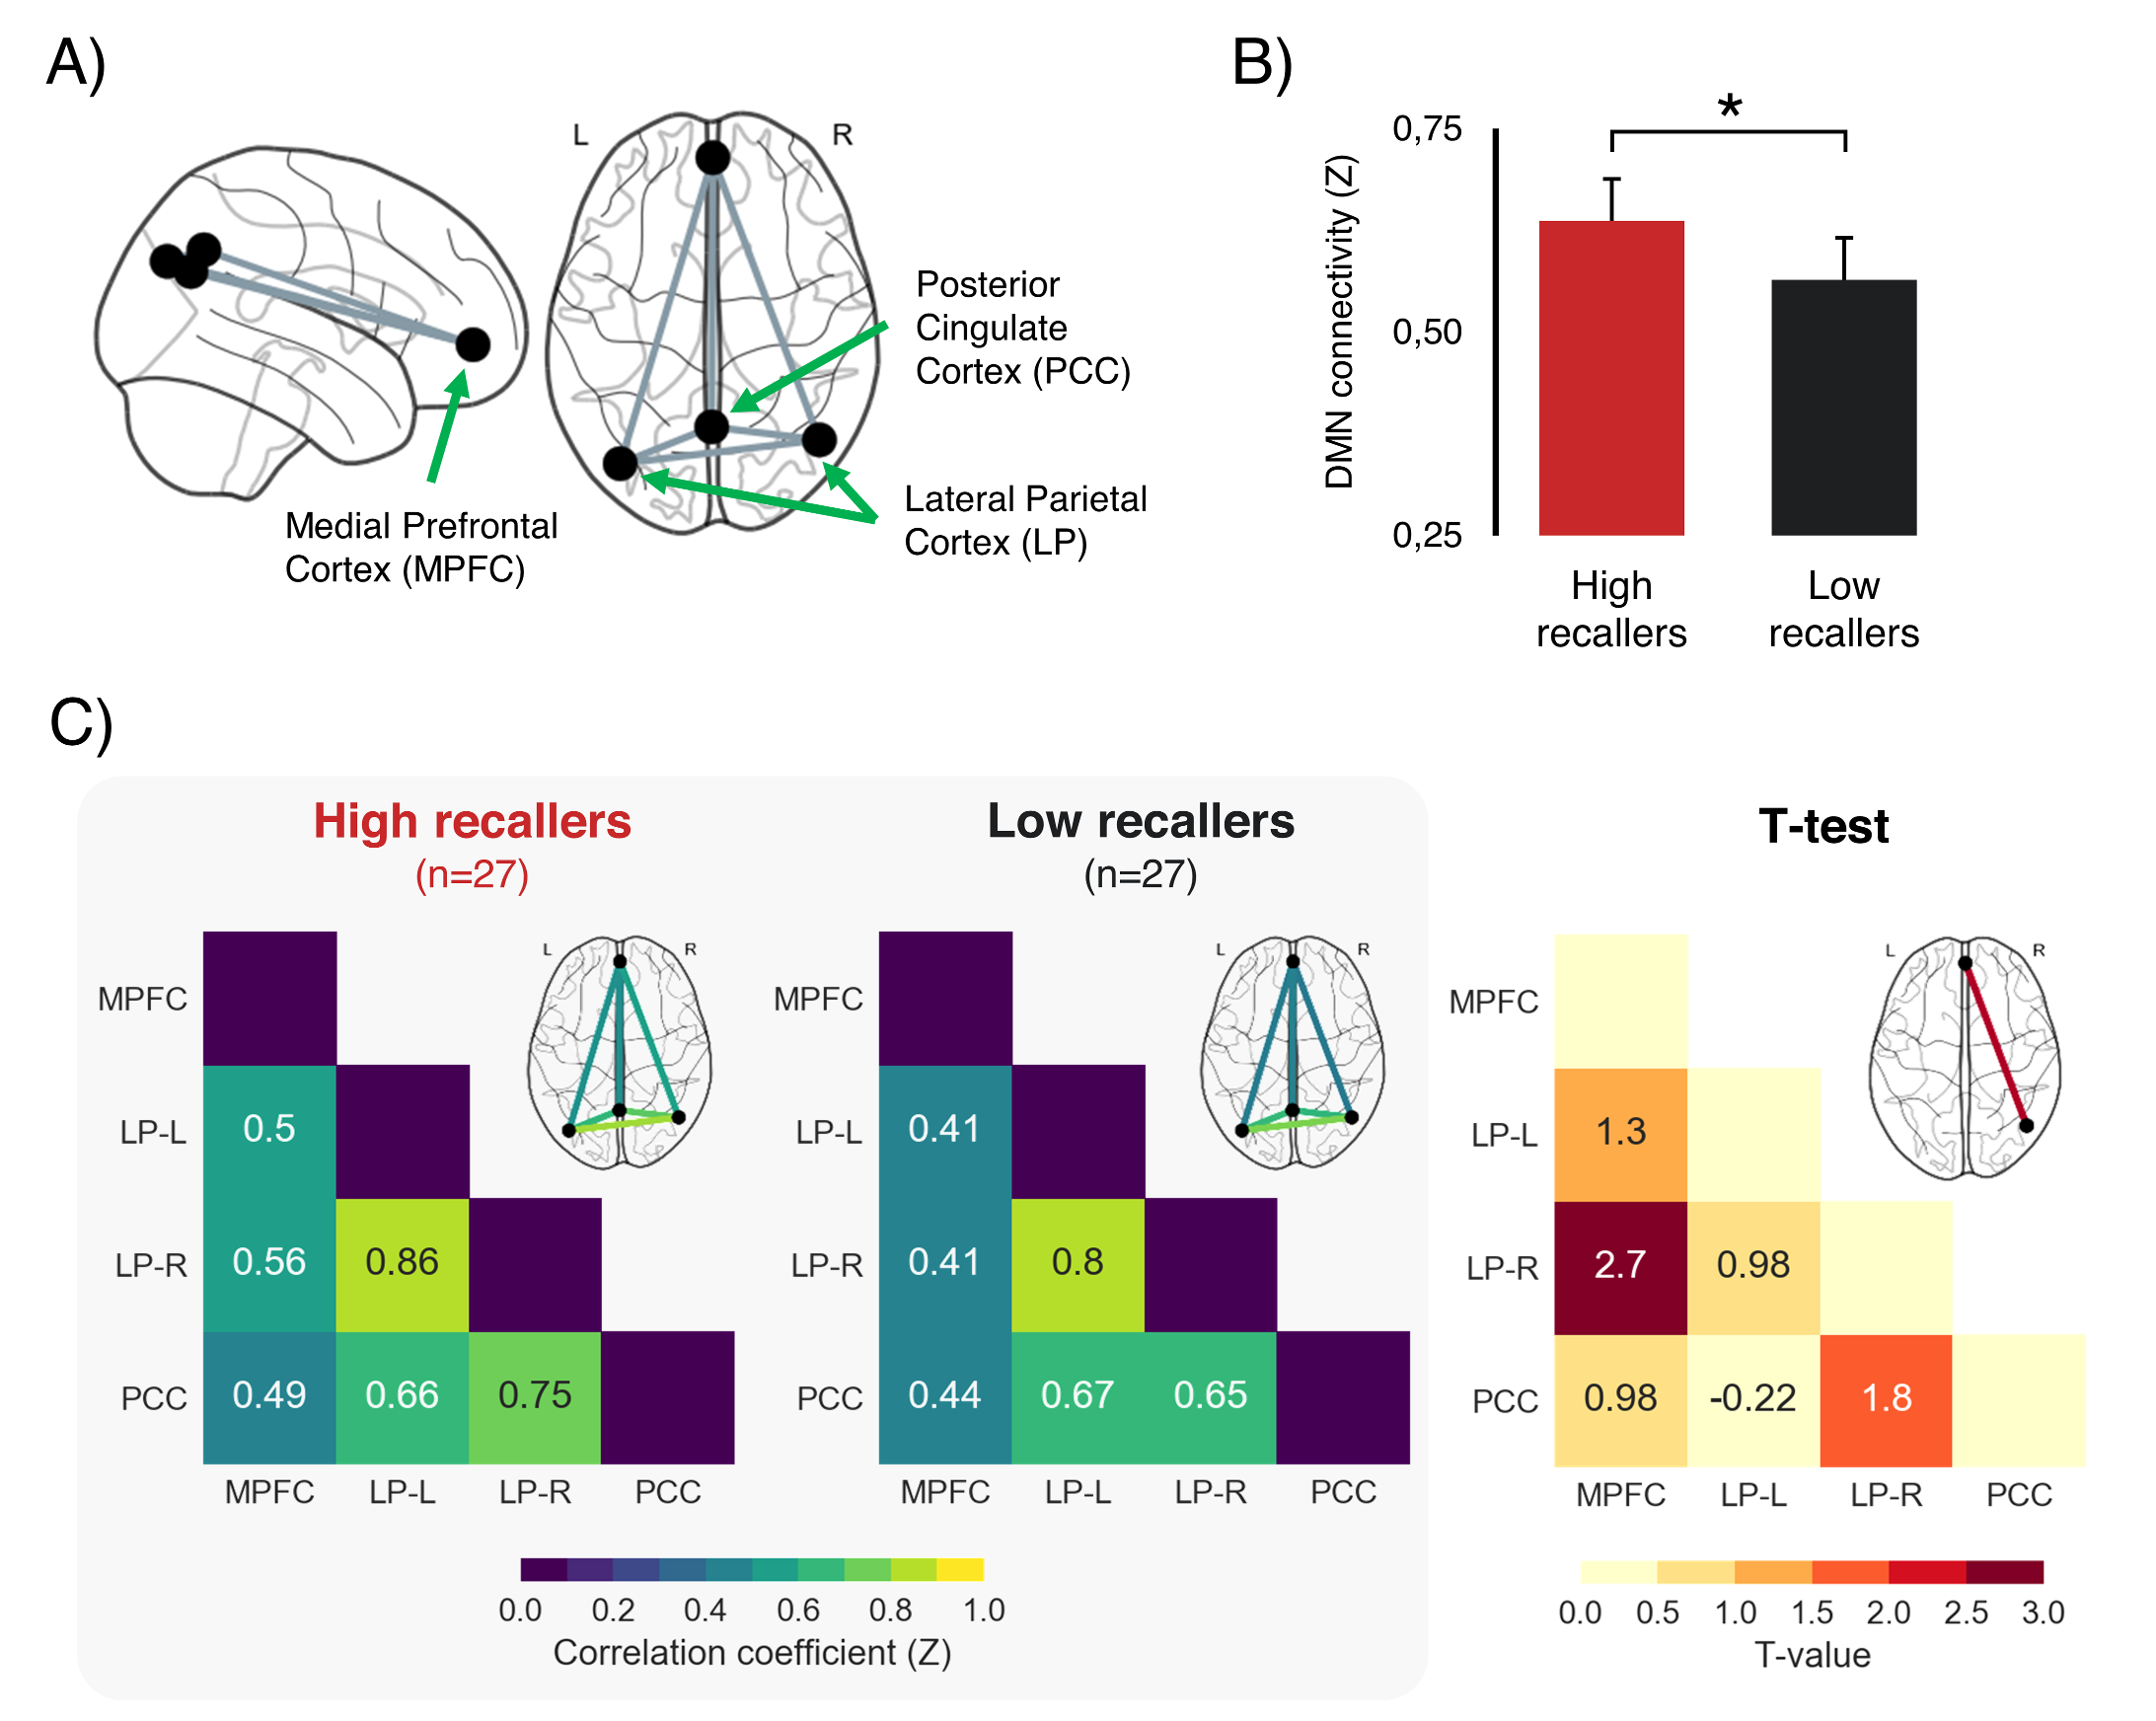
\includegraphics[width=\textwidth]{Fig/Results/Inertia/Creativity/Fig1.png}
	\caption*{\textbf{Fig 1. Increased default mode network connectivity in High dream recallers (HR) compared to Low dream recallers (LR).} (A) Schematic illustration of the four main nodes of the default mode network (DMN) included in further connectivity analysis. (B) Mean pairwise connectivity of the DMN for HR (red) and LR (black), obtained by averaging for each subject all the pairwise correlation values within the default network. The average DMN connectivity was significantly higher in HR than in LR. Error bars represent 95\% confidence intervals. (C) Left grey panel. Functional connectivity matrix representing the mean pairwise correlation coefficient between regions of the DMN in HR and LR. Right. Between-group statistical comparison (two-sided T-test corrected for multiple comparisons using the false discovery rate). The connectivity between the right lateral parietal and medial prefrontal cortex was significantly higher in HR than in LR.}
\end{figure}

\begin{figure}[!htbp]
	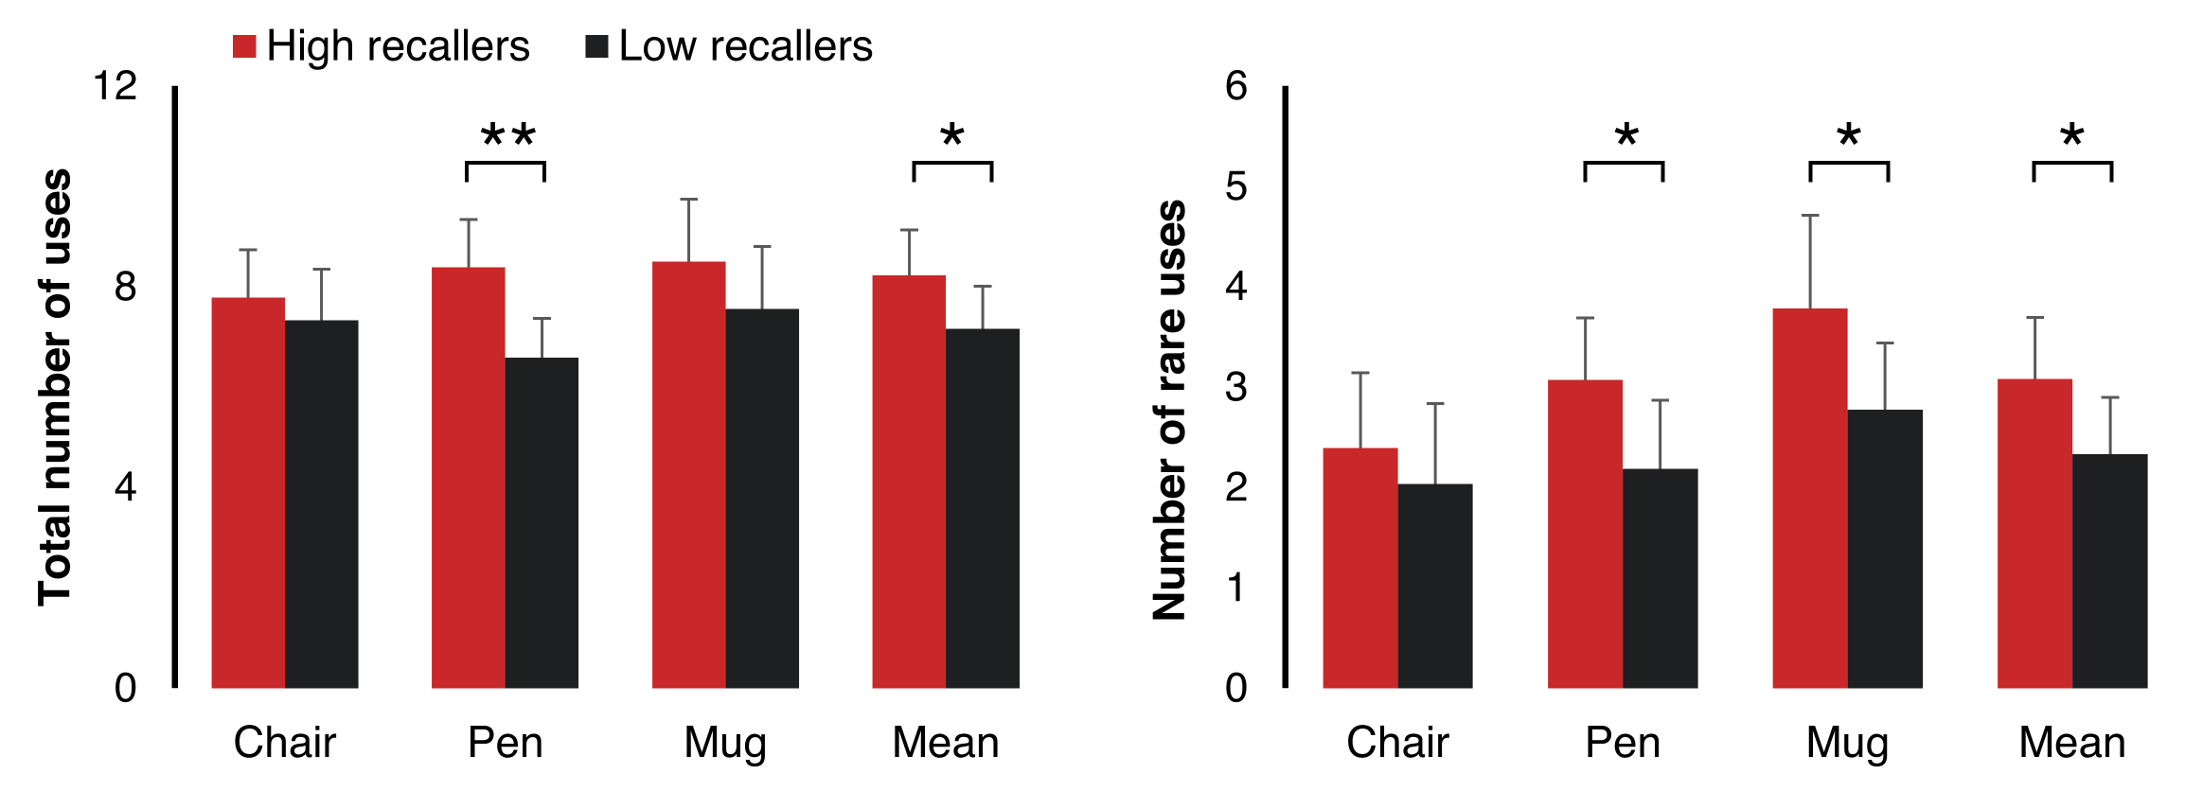
\includegraphics[width=\textwidth]{Fig/Results/Inertia/Creativity/Fig2.png}
	\caption*{\textbf{Fig 2. Higher creativity in High dream recallers (HR) than in Low dream recallers (LR).} \emph{Left}. Group means for the total number of uses found by HR (red) and LR (black) during the Guildford’s alternate uses task. HR reported significantly more uses than LR for the “pen” object and in average (“mean” column). \emph{Right}. Group means for the number of uses reported by 5 or less participants (i.e. top 10\% rarest uses). HR reported significantly more rare uses than LR for the “pen” and “mug” objects, as well as in average (“mean” column). Error bars represent 95\% confidence intervals. *p<.05.}
\end{figure}

% \FloatBarrier

\subsection*{Discussion}
\label{res:dmn-crea:discussion}

This study reports for the first time the brain functional connectivity correlates of DRF in healthy subjects. The results presented above indicate that HR have an increased brain functional connectivity within the DMN, notably between the MPFC and TPJ. In addition HR scored higher than LR on measures of creative-idea generation, without any further between group differences in cognitive or memory abilities.

With regards to functional connectivity, our results are remarkably consistent with a previous PET study from our team that showed, in an unrelated sample of 41 participants, a higher rCBF in HR compared to LR in these two same regions during both sleep and wakefulness \citep{eichenlaub_resting_2014}. Both these studies are in accordance with clinico-anatomical reports showing that lesions in the TPJ and the MPFC lead to a cessation of dream reporting \citep{solms_neuropsychology_1997}. Our results provide therefore strong evidence that the ability to recall dreams is linked to rCBF and functional connectivity in these two brain regions. Noteworthy, the finding of a higher functional connectivity in regions that were previously reported to demonstrate an higher rCBF is not surprising given the results of previous studies that reported a tight coupling between blood supply and brain functional connectivity \citep{liang_coupling_2013}.

Furthermore, our findings confirmed previous studies reporting a positive link between creativity and DRF \citep{fitch_variations_1989, schredl_creativity_1995, schredl_factors_2003}. This is of particular interest given that the generation of creative ideas is thought to be also supported by a preferential recruitment of regions of the DMN, and particularly of the MPFC \citep{dietrich_review_2010, ellamil_evaluative_2012, jung_structure_2013, beaty_creativity_2014, mok_interplay_2014, beaty_default_2015}. This large overlap of brain regions involved in dreaming and creativity was noticed by \citet{christoff_mind-wandering_2016} who postulated that creative thought and dreaming are best understood as members \q{of a family of spontaneous-thought processes}. This idea was put slightly differently by \citet{barrett_dreams_2017} who stated that \q{dreaming is essentially our brain thinking in another neurophysiologic state—and therefore it is likely to solve some problems on which our waking minds have become stuck}. Several studies have indeed reported that dream content \emph{per se} often contains solutions of unsolved problems (hence the famous saying \q{sleep on it};  \citealp{dement_relation_1957, barrett__1993}).

Taking this line of thought further, we argue here that high frequency dream recallers have a specific cognitive and functional profile, involving greater baseline activity in regions of the DMN, which might in turn promote in these individuals creativity and dreaming abilities. Further evidence that HR and LR have a differential neurophysiological profile is provided by recent works from our team showing that HR demonstrated a larger amplitude of brain responses to auditory novel stimuli than LR during both a night of polysomnographically recorded sleep and wakefulness, as well as an increased duration of intra-sleep wakefulness (~15 min more on average) and nocturnal awakenings, regardless of the previous sleep stage, and without any other differences in the micro- or macro-structure of sleep \citep{eichenlaub_brain_2014, vallat_increased_2017}.

Along with the consistent positive association between DRF and creativity, studies have often reported a substantial correlation between DRF and personality traits, such as openness to experience \citep{schredl_dream_2003}, thinner boundaries (i.e. propensity to being more open, trustworthy, vulnerable, and sensitive; \citealp{hartmann_boundaries_1989, schredl_dreaming_1996}), and anxiety \citep{schonbar_manifest_1959, tart_frequency_1962}. None of these variables were statistically different between HR and LR in the present study but it is noteworthy that HR scored higher for all of these variables and some of them were close to significance. Since the above-mentioned correlations have often been reported on larger samples, one can assume that the group differences on these variables would have been significant if our study involved a larger sample of participants. The general idea that differential DRF is linked to traits factors was first introduced by \citet{schonbar_differential_1965} in her so-called \q{life-style} hypothesis. While she did not explained the underlying mechanisms, she postulated that high dream recall is part of a general life style characterized by \q{creativity, rich fantasy, introversion, introspection, field independence and divergent thinking} \citep{schredl_dream_1999}. Our findings argue in favor of this model and provide evidence for a brain mechanism promoting in HR dreaming and creativity.

Future researches should investigate whether this brain mechanism could also explain intra-individual variability in DRF across time. For instance, it seems fruitful to test whether DRF enhancing methods (such as keeping a dream diary; \citealp{schredl_questionnaires_2002}) would result in increased creativity scores and DMN functional connectivity in post compared to pre-training measures within the same individuals (preferentially a group of LR).

% \paragraph{Acknowledgments}
% The authors would like to thank Basak Turker, Morgane Hamon, Franck Lamberton and Danielle Ibarrola for substantial help in data collection and analysis, as well as Jamila Lagha for her help in administrative work.
%
% \paragraph{Author contribution}
% R.V and P.R designed the survey, RV collected, analyzed the data and wrote the first draft. All authors were involved in the writing process.

\cleardoublepage

\chapter{Study 4. Sleep and dream habits in a sample of French students}
\label{res:survey}

\cleardoublepage

\textbf{{\large Sleep and dream habits in a sample of French students}}

\hfill Under review at \emph{Journal of Sleep Research}

\bigskip

Raphael Vallat\textsuperscript{1} (PhD candidate), Mickael Eskinazi\textsuperscript{1} (PhD), Alain Nicolas\textsuperscript{1,2} (M.D, PhD), Perrine Ruby\textsuperscript{1} (PhD)

\textsuperscript{1} Lyon Neuroscience Research Center, Brain Dynamics and Cognition team, INSERM UMRS 1028, CNRS UMR 5292, Université Claude Bernard Lyon 1, Université de Lyon, Lyon, France

\textsuperscript{2} Unité Michel Jouvet, Centre Hospitalier Le Vinatier, 95 boulevard Pinel, Lyon, France

\subsection*{Summary}
\label{res:survey:summary}

Several authors have drawn the attention to the risk of sleep difficulties during college years. However, sleep and dream habits have been scarcely documented in young adults. We collected such information in a sample of 1137 French college students (411 males). In average, the participants reported spending roughly 8 hours in bed during weekdays, 9 hours during the weekends, and 90.9\% reported no difficulty to fall asleep. The mean sleep agitation score reported was 3.3 ± 1.7 (1-to-10 scale). Less than 0.4\% of students reported to have sleep-walking episodes regularly but nearly 7\% reported regular sleep-talking episodes. About 10\% reported to often take a nap. In average, participants mentioned 3 dream reports per week, 14\% said they had frequent lucid dreams and 6\% reported frequent recurrent dreams. The clarity of dream memory was positively correlated with dream recall frequency. An academic field effect (humanities, science, medicine) has been found for sleep duration. By contrast, no DRF differences were observed between disciplines. We observed the well-known negative correlation between age and dream recall frequency despite a limited age range, as well as a gender effect for several sleep and dream parameters. As compared to men, women spent more time in bed and reported slightly more dreams. These results (1) suggest that the great majority of French college students do not suffer from sleep disturbances, (2) show a gender difference for several sleep parameters and (3) provide supplementary arguments in favor of a small but consistent gender effect regarding dream recall frequency.

\paragraph{Keywords}
Sleep habits, dream recall frequency, students, survey, epidemiology, gender differences

\subsection*{Introduction}
\label{res:survey:intro}

Recent years have witnessed a renewed interest in sleep and dreaming \citep{dijk_dreaming_2015}. However, epidemiological investigations in healthy subjects combining questions on both sleep and dream habits are relatively rare. Such surveys are yet necessary to establish and keep up to date sleep and dream norms in the general population. Of particular interest is the college population, which is more at risk of suffering from sleep difficulties than the general population \citep{buboltz_sleep_2001, curcio_sleep_2006, forquer_sleep_2008, lund_sleep_2010}. Yet, there are few, up-to-date, data available on sleep habits of college students. This is especially true for the European college population since most epidemiological studies have been carried out on Americans (e.g. \citealp{lund_sleep_2010}). By contrast, dream habits of college students have been more investigated, especially by Mickael Schredl who extensively reported the dream patterns of German students. Yet, most surveys on dream habits were conducted on psychology students \citep{schredl_factors_2003}, and are therefore not necessarily representative of the student population since there is a great majority of women in this academic field. This point is not negligible given that several studies suggest a gender effect in sleep and dream habits \citep{beck_insomnia_2013, schredl_gender_2008}. It is important to note however, that regarding DRF the effect was not always reproduced and the overall effect size is small.

The originality of our study is to provide recent (2016) sleep and dream habits from a large sample (n = 1137) of French college students (Lyon University) pertaining to various academic fields (i.e. humanities, sciences, medicine), and composed for one third by males (n = 411). The web questionnaire asked about habitual time of light extinction and awakening during the week and the week-end, ability to fall asleep, sleep agitation, nap frequency, sleepwalking, sleep-talking, dream recall frequency, clarity of dream content, frequency of lucid and recurrent dreams. In addition to the descriptive aim of the study, we expected to reproduce results reported in previous surveys such as the correlation between age and DRF \citep{schredl_dream_2008}, or between DRF and the clarity of the dream memory, and a gender effect on sleep and dream parameters.

\subsection*{Methods}
\label{res:survey:methods}

Data were collected in 2016 using an online questionnaire for the recruitment phase of an fMRI sleep study. The subjects were informed of the study through an announcement sent to several mailing lists of Lyon University. Among with basic sociodemographic variables (age, gender, height, weight, education, academic discipline), the online survey included the following questions:

\begin{my_list_num}
    \item What time do you usually go to bed and get up during weekdays?
    \item What time do you usually go to bed and get up during weekends?
    \item In general, you fall asleep: very easily, easily, quite easily, with difficulty or with great difficulty?
    \item On a scale of 1 to 10, how much agitated is your sleep? (1 = not at all agitated, 10 = very agitated)
    \item How often do you experience sleepwalking episode? (never, rarely, sometimes, often)
    \item How often do you talk during your sleep? (never, rarely, sometimes, often)
    \item How often do you take daytime nap? (never, rarely, sometimes, often)
    \item How many days per week do you usually wake up with a dream in mind?
    \item How many days per month do you usually wake up with a dream in mind?
    \item How often do you have lucid dream(s) (i.e. dreams in which you are aware that you are dreaming)? (never, rarely, sometimes, often)
    \item How often do you have recurrent dream(s) (i.e. dream experienced repeatedly)? (never, rarely, sometimes, often)
    \item In general, how clear is the memory of your dream content? (very vague, vague, clear, very clear)
\end{my_list_num}

We collected 1262 completed questionnaires (459 M, age range = 18 - 61 yr., mean age ± SD = 22.75 ± 3.94 yr.). In order to be representative of a student population, participants older than 30 years were removed, leading to a final sample size of 1137 (411M - 726 F, mean age ± SD  = 22.23 ± 2.36 yr., height = 170.2 ± 11.4 cm, weight = 64.1 ± 11.6 kg, education = 3.3 ± 1.8 years after high school). A binomial logistic regression was performed to investigate the gender differences in sleep and dream habits. In order to be entered in the model, the frequency of sleepwalking and sleep-talking episodes, and the frequency of lucid and recurrent dreams were recoded as follows: Never → 0, Rarely → 1, Sometimes → 2, Often → 3. The dream clarity scale was recoded using: Very vague → 0, Vague → 1, Clear → 2, Very clear → 3.  The level of ease or difficulty to fall asleep was recoded using: very easily → 0, easily → 1, quite easily → 2, with difficulty → 3, with great difficulty → 4. Finally, we compared the sleep and dream habits of students as a function of the academic discipline. We partitioned the sample in three broad categories, namely sciences (i.e. hard sciences and technology, n = 432 students), humanities (i.e. social sciences, literature, psychology, educational science, law school, n = 417 students) and medicine (i.e. medical and dental studies, n = 190). The 98 remaining students of the sample were not included in the analysis because they were issued from heterogeneous academic and/or professional environment.

\subsection*{Results}
\label{res:survey:results}

\subsubsection*{Sleep habits}
The average time in bed was 7.90 ± 0.96 hours (range = 3.5 - 12 hours) during weekdays and 9.10 ± 1.13 hours (range = 4 - 13 hours, paired t-test = <.001) during weekends. Sleep schedules during weekdays and weekends are reported in Fig 1. The peak bedtime was between 11 and 11.59 pm (43.4\%) during weekdays and between 0 and 0.59 am during weekends (33.57\%). The peak waking time was between 7 and 7.59 am during weekdays (42.33\%) and between 10 and 10.59 am during weekends (29.96\%).

\begin{figure}[htb]
	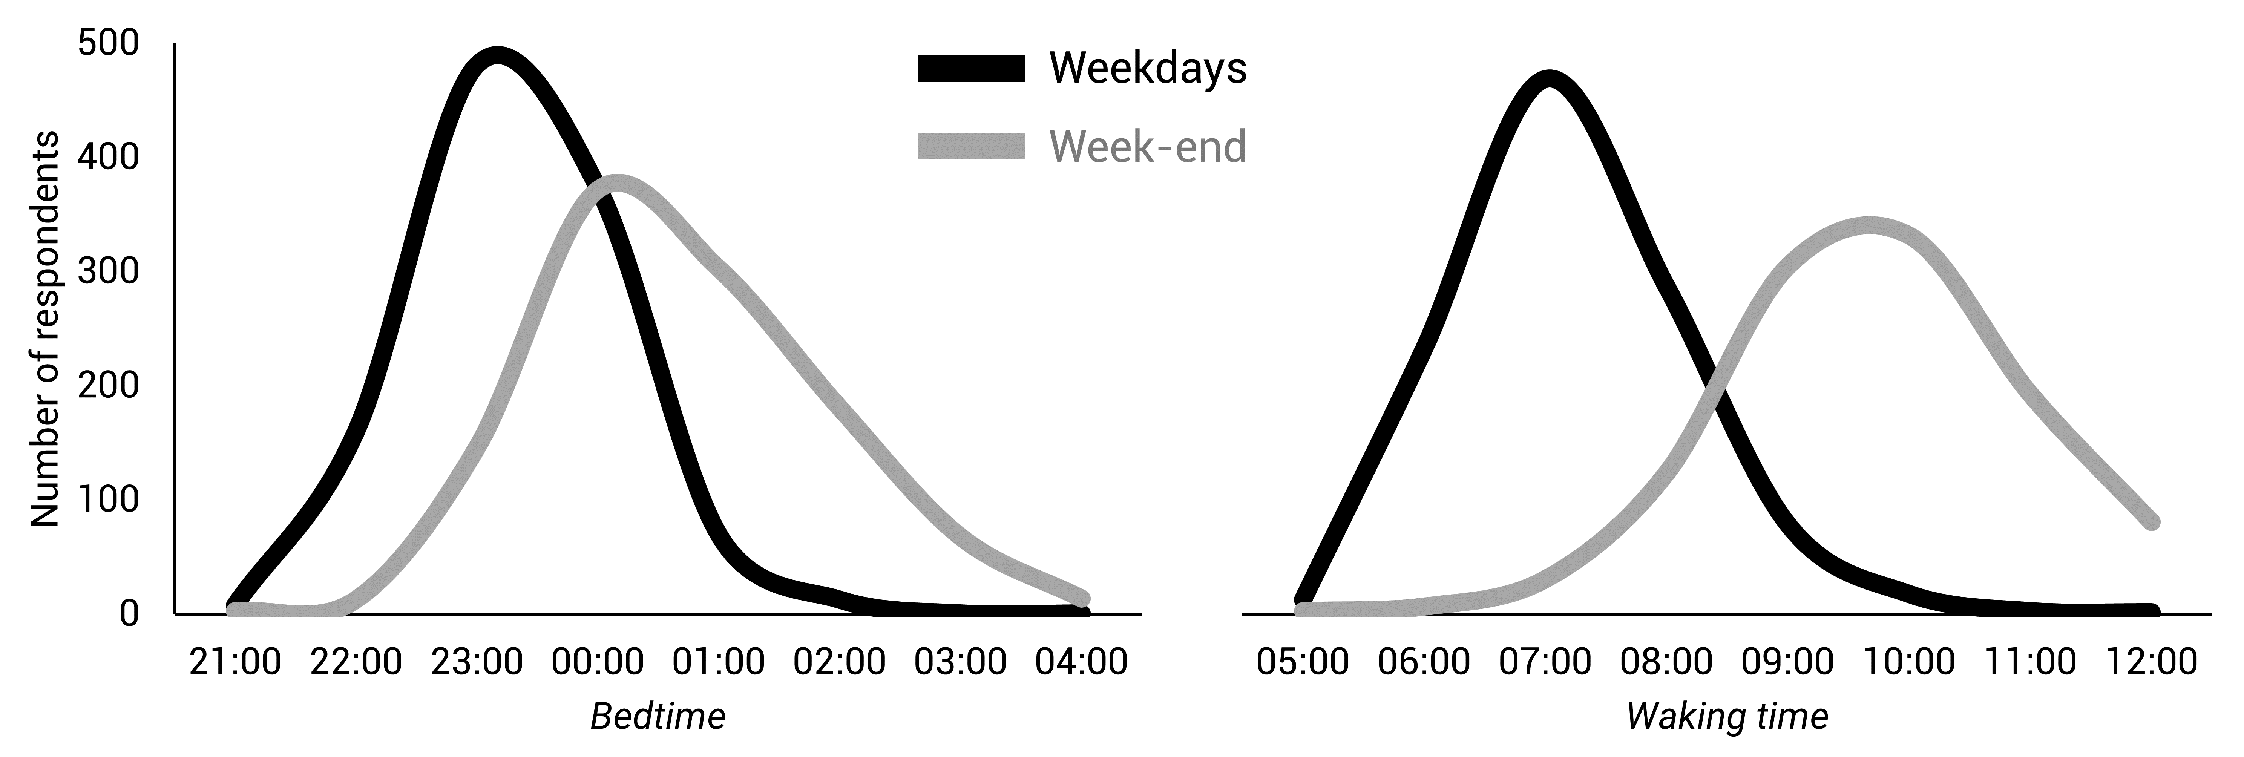
\includegraphics[width=\textwidth]{Fig/Results/Survey/Fig1.png}
	\caption*{\textbf{Fig 1.} Bedtime (left) and waking time (right) distribution during weekdays (black lines) and weekends (grey lines).}
\end{figure}

Only 4 respondents (0.35\%) reported having great difficulty falling asleep. Conversely, 429 students (37.7\%) reported falling asleep easily and 184 (16.18\%) reported falling asleep very easily. The mean sleep agitation score reported was low (3.3 ± 1.7). Regarding sleepwalking, only 4 students (0.35\%) reported having regular episodes, while 986 (86.72\%) of them reported never having episodes. The percentage of students reporting regular episodes of sleep-talking was higher (75 students, 6.6\%), and only 315 respondents (27.7\%) declared never having sleep-talking episodes. Finally, a total of 113 participants (9.94\%) reported that they often took nap, while 196 respondents (17.24\%) reported that they never took nap. Frequencies of nap, sleepwalking, sleep-talking, recurrent dreams and lucid dreams are reported in Fig 2.

\begin{figure}[htbp]
	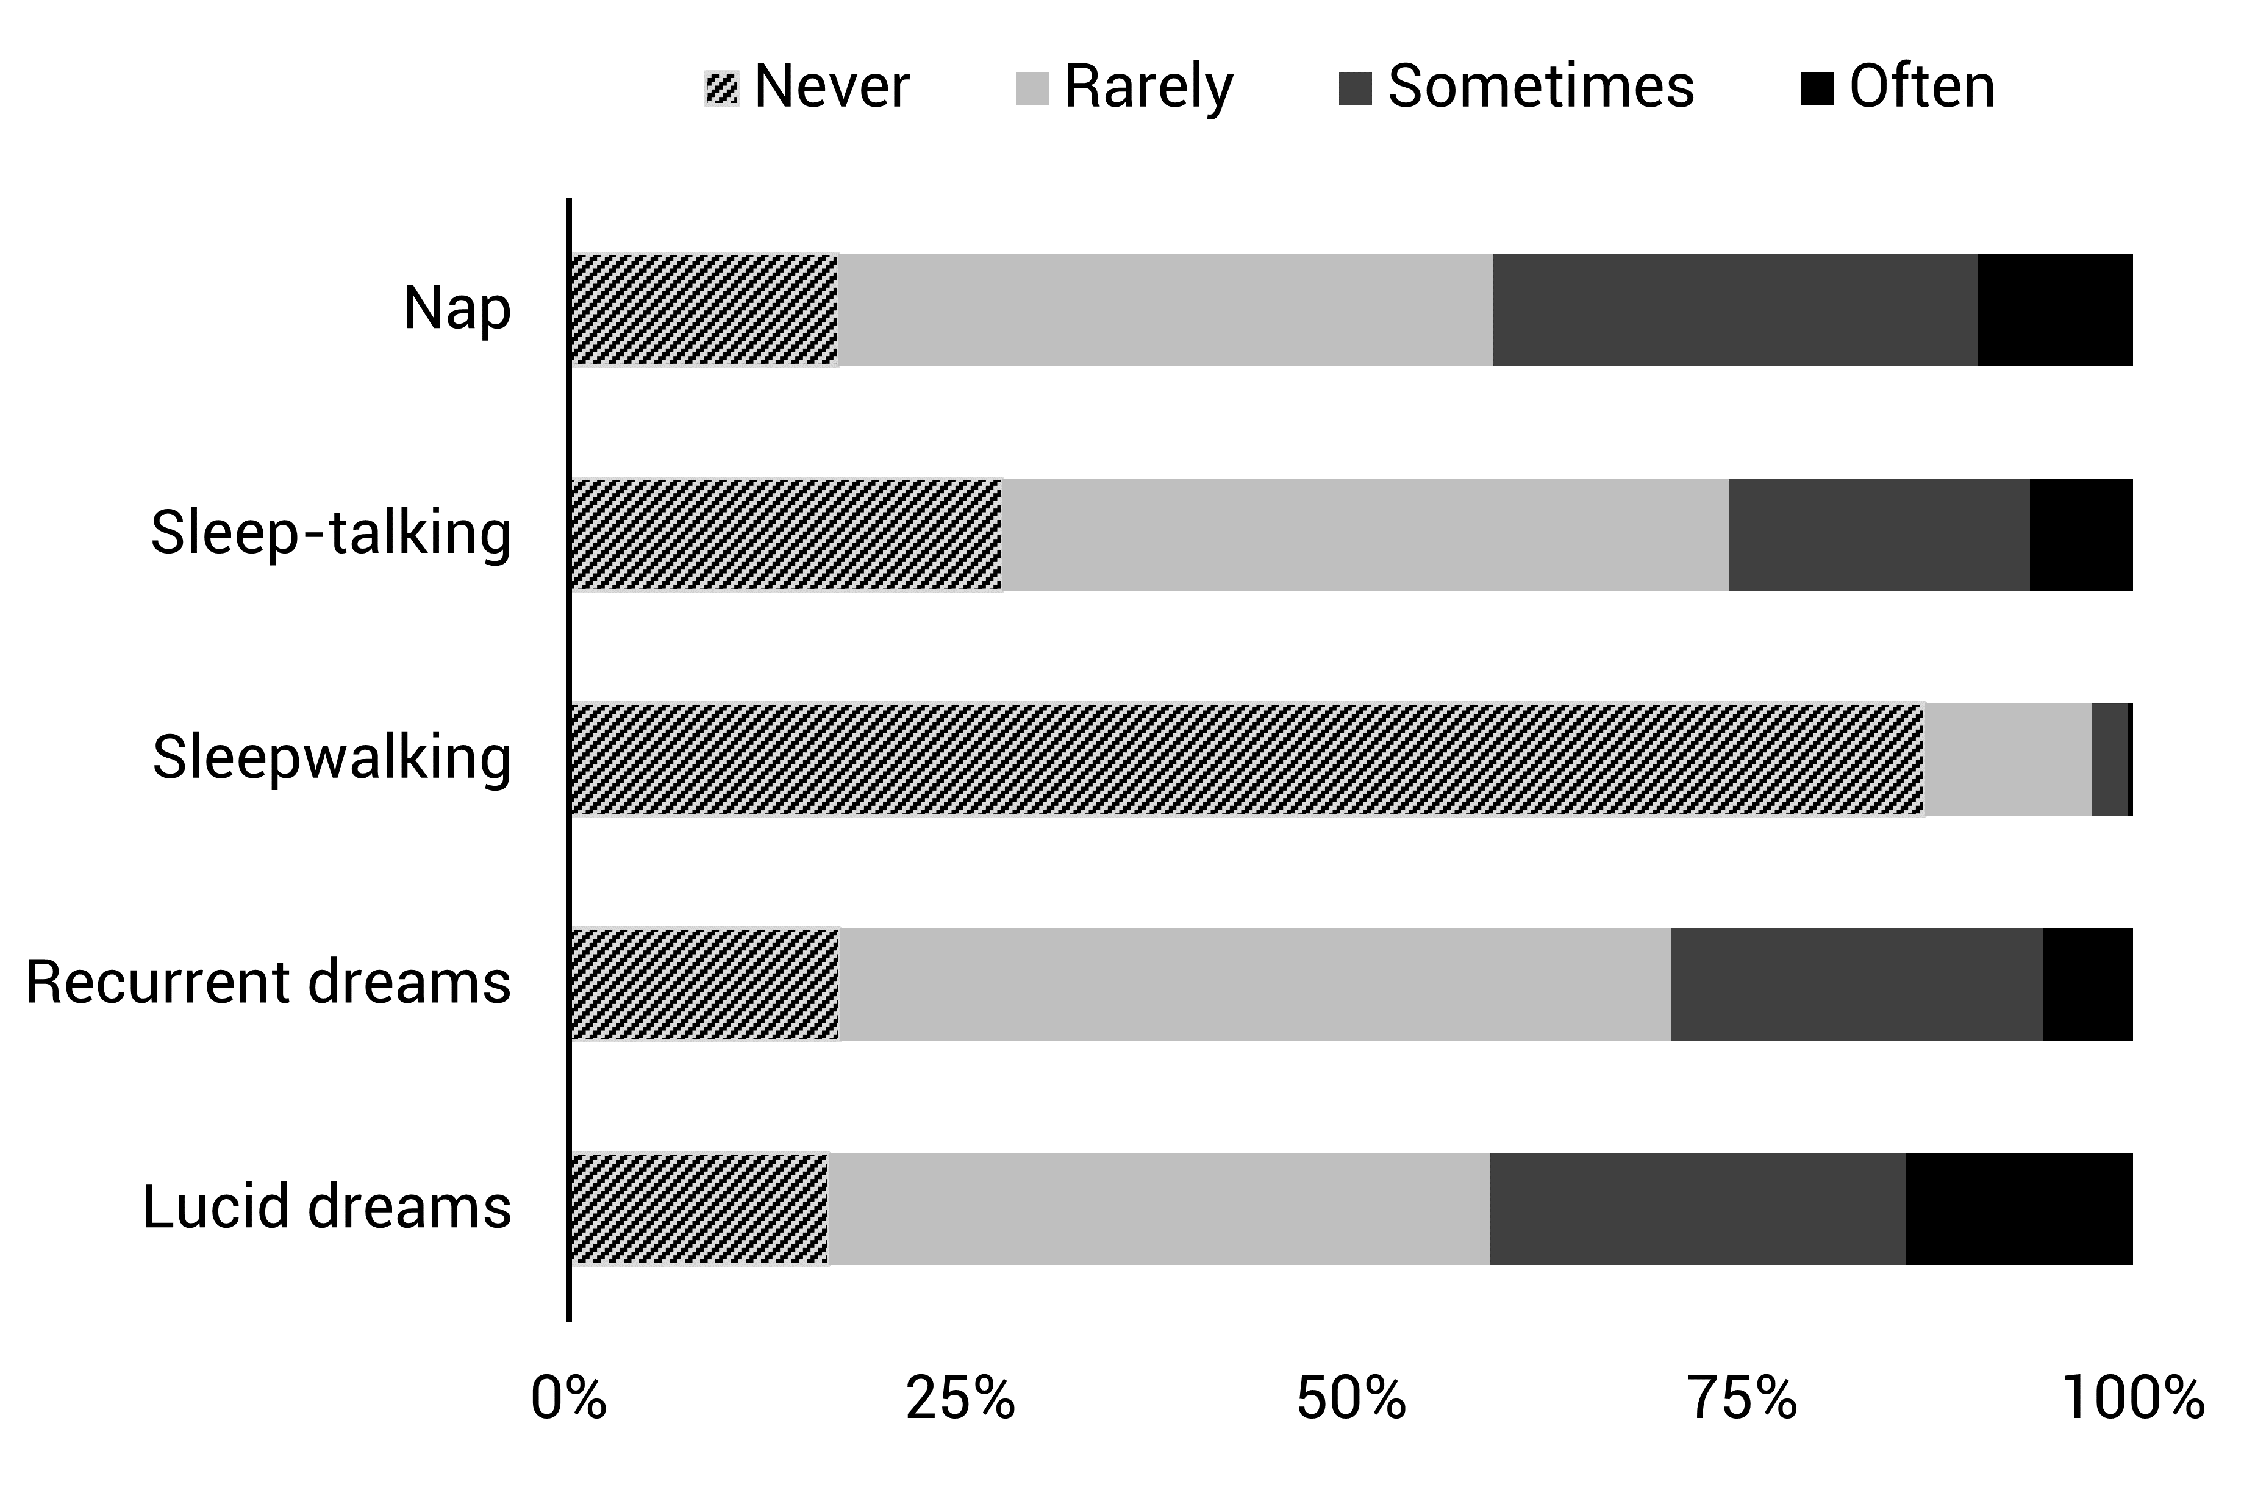
\includegraphics[width=\textwidth]{Fig/Results/Survey/Fig2.png}
	\caption*{\textbf{Fig 2.} Frequencies of nap, sleep-talking, sleepwalking, recurrent dreams and lucid dreams in the sample.}
\end{figure}

\subsubsection*{Dream recall frequency}
The mean dream recall frequency (DRF) was 3.12 ± 1.78 days per week (i.e. the participants recalled a dream in average 3 mornings per week) and 12.84 ± 7.51 days per month. Fifty-eight participants (5.10\%) reported not recalling any dream per week and 9 participants (0.79\%) reported not recalling any dream per month. On the opposite, 34 participants (2.99\%) reported recalling a dream 7 mornings per week and 29 participants (2.55\%) reported recalling a dream every morning of the month.

Despite the narrow age range of our sample (18 to 30 years old), we were able to evidence the negative correlation between DRF (weekly estimation) and age (Fig 3A) evidenced in previous studies with a larger range (e.g. \citealp{schredl_dream_2008}). Weekly DRF was positively correlated with the frequency of lucid dreams (Fig 3C), as could be expected from previous results \citep{stepansky_austrian_1998, schredl_lucid_2004, schredl_frequency_2011}. Weekly DRF was also positively correlated with the clarity of dreams (Fig 3D) and the level of agitation during sleep (Pearson r = 0.08, p = 0.008). We observed neither an effect of the academic field on DRF, nor a significant correlation between DRF and the education level (Fig 3B). These findings are consistent with two studies that reported no association between DRF and the education level and DRF and the socioeconomic status \citep{schredl_dream_2007, schredl_dream_2008}.

\begin{figure}[htbp]
	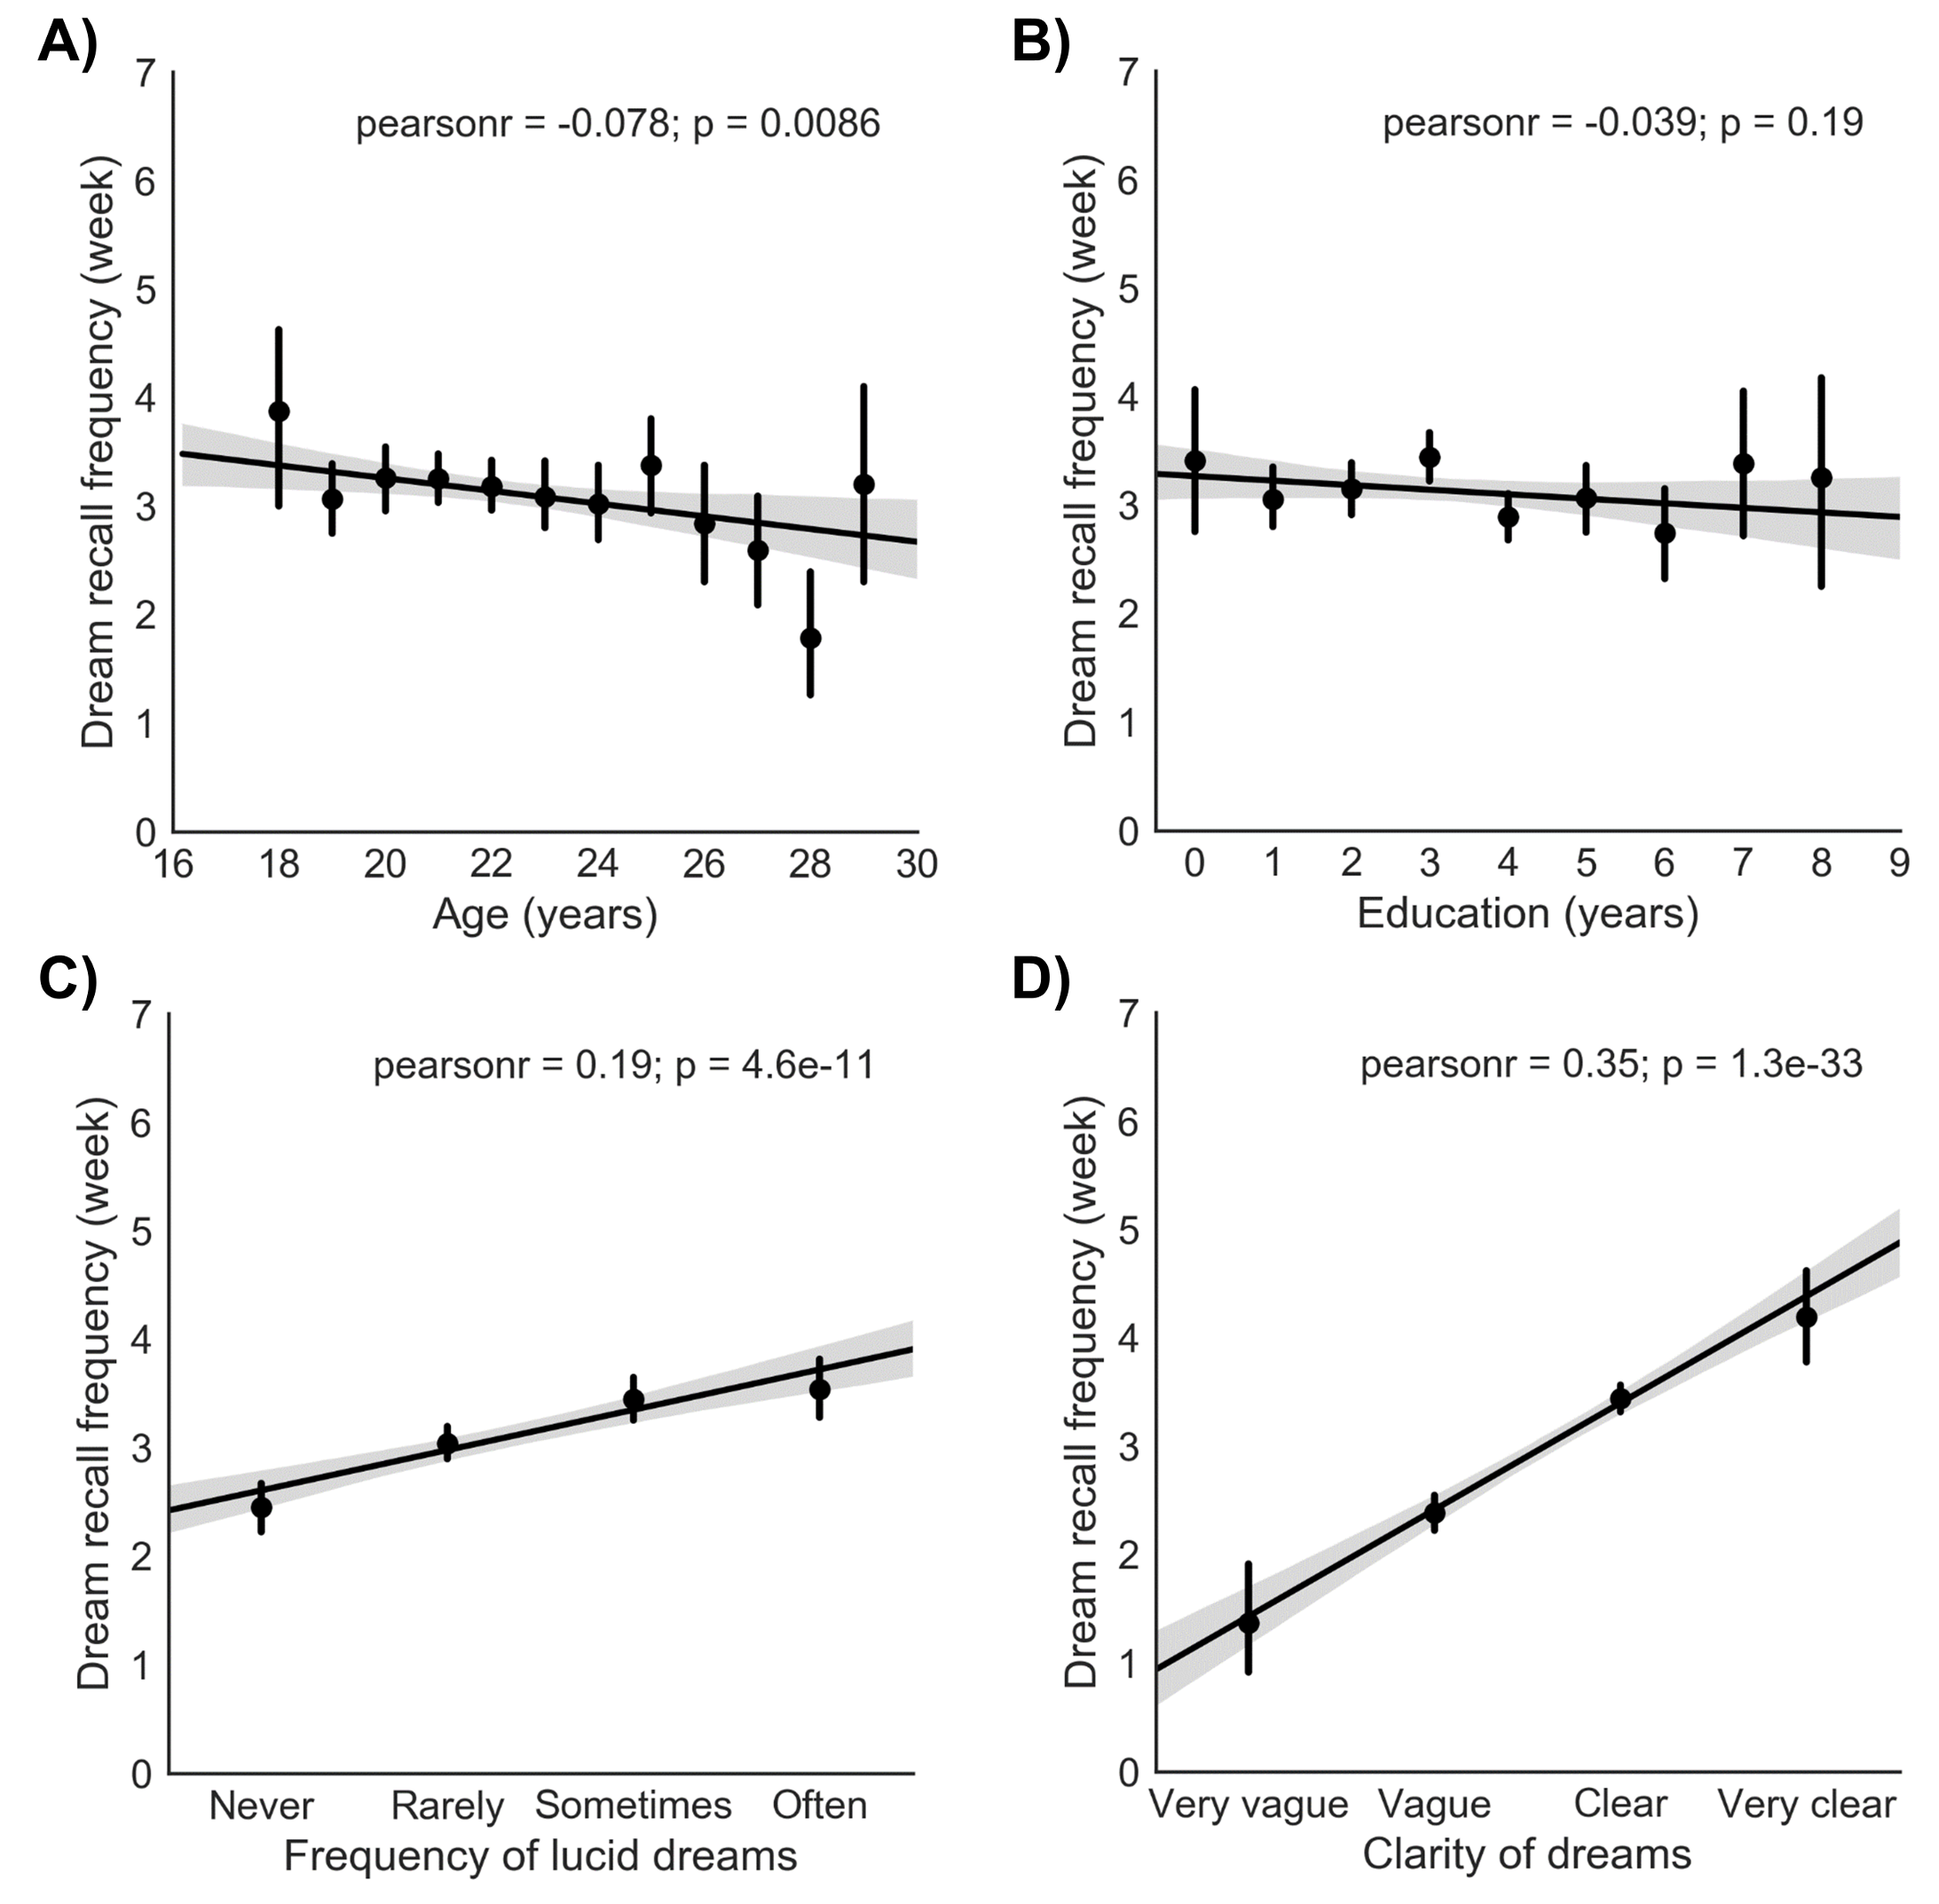
\includegraphics[width=\textwidth]{Fig/Results/Survey/Fig3.png}
	\caption*{\textbf{Fig 3.} Correlations between dream recall frequency (number of mornings per week with a dream in mind) and (A) age (B) education level (C) frequency of lucid dreams (D) clarity of dream memory. Error bars represent 95\% confidence intervals.}
\end{figure}

\paragraph{Clarity of dreams}
Thirty-five participants (3.08\%) reported that the usual clarity of their dreams was very vague. By contrast, 75 participants (6.60\%) reported that their dreams were usually very clear. The great majority of respondents (n=705, 62.0\%) reported that their dreams were usually clear.

\paragraph{Frequency of lucid dreams}
A lucid dream is a dream during which the dreamer is aware of dreaming. In our sample, 165 participants (14.51\%) reported that they often had lucid dreams, while 189 participants (16.62\%) reported that they never had a lucid dream (Fig 2). From these figures, it could be inferred that approximatively 83\% of the participants have already experienced a lucid dream at least once. This number is remarkably consistent with those from other studies focusing on student population (e.g. 82\% in \citealp{schredl_lucid_2004}). However, it should be noted that the definition of lucid dreaming given in the questionnaire did not include the ability to control the dream characters and narratives, but simply to be aware of dreaming during the dream. It is generally admitted that control over the dream represents the full extent of lucid dreaming and is more difficult to attain than the mere awareness of dreaming \citep{purcell_dream_1986, laberge_exploring_1991}. Consequently, the proportion of participants having already experienced a lucid dream would probably be lower if the definition of lucid dreaming involved the ability to exert some degree of control over the dream.

\paragraph{Frequency of recurrent dreams}
A recurrent dream is a dream which is experienced repeatedly. In our sample, 65 participants (5.72\%) reported that they often had recurrent dreams, while 197 participants (17.33\%) reported that they never had a recurrent dream (Fig 2), meaning that roughly a little more than 80\% of the participants had already experienced recurrent dreams at some point in their lives. Again, this figure is consistent with several studies that reported a prevalence of 60\% to 75\% of recurrent dreams in college students and young adults \citep{zadra_recurrent_1996}.

\subsubsection*{Gender differences}
Table 1 depicts the summary of the binomial logistic regression for gender differences. In our sample, as compared to men, women spend more time in bed (during both weekdays and weekends), take naps more often, are more susceptible to have episodes of sleepwalking, and have a higher weekly-estimated DRF. Women tend also to have a more agitated sleep and to report more difficulties to fall asleep. Finally, the frequency of lucid dreams tends to be higher in men, while the frequency of recurrent dreams tends to be higher in women.

\begin{table}[!htbp]
    \caption*{\textbf{Table 1. Binomial logistic regression for gender differences in sleep and dream habits (n=1137).} SE = standardized estimate, DRF = dream recall frequency. Frequencies of nap, sleepwalking, sleep-talking, recurrent dreams and lucid dreams are expressed using a recoded scale ranging from 0 (Never) to 3 (Often). Sleep agitation is scored on a 1-to-10 scale where 1 means no agitation at all during sleep and 10 means a very agitated sleep. Difficulty falling asleep is expressed using a recoded scale ranging from 0 (very easy to fall asleep) to 4 (very difficult to fall asleep). For sleep agitation and difficulty to fall asleep, higher scores indicate more disturbances.}
    \begin{tabularx}{\textwidth}{lllXXX}
    \toprule
    Variable                       & Men                       & Women         & SE    & X²    & p        \\ \midrule
    \emph{Sleep}                   &                           &               &       &       &          \\
    Time in bed (weekdays)         & 7.70 ± 1.0                & 8.02 ± 0.9    & 0.31  & 28.92 & .001     \\
    Time in bed (weekends)         & 8.93 ± 1.2                & 9.19 ± 1.1    & 0.13  & 5.14  & .023     \\
    Difficulty falling asleep      & 1.35 ± 0.9                & 1.42 ± 0.9    & 0.14  & 3.61  & .057     \\
    Sleep agitation                & 3.13 ± 1.6                & 3.39 ± 1.8    & 0.07  & 2.87  & .090     \\
    Frequency of nap               & 1.24 ± 0.9                & 1.39 ± 0.8    & 0.23  & 9.31  & .002     \\
    Frequency of sleepwalking      & 0.12 ± 0.4                & 0.19 ± 0.5    & 0.33  & 4.02  & .045     \\
    Frequency of sleep-talking     & 1.04 ± 0.9                & 1.05 ± 0.8    & -0.11 & 0.61  & 0.43     \\
    \emph{Dream}                   &                           &               &       &       &          \\
    DRF (weekly)                   & 2.83 ± 1.7                & 3.29 ± 1.8    & 0.10  & 15.50 & .001     \\
    DRF (monthly)                  & 11.60 ± 7.3               & 13.54 ± 7.5   & 0.01  & 0.18  & .663     \\
    Dream clarity                  & 1.69 ± 0.6                & 1.74 ± 0.6    & -0.04 & 0.16  & .689     \\
    Frequency of recurrent dreams  & 1.09 ± 0.8                & 1.23 ± 0.8    & 0.14  & 2.77  & .096     \\
    Frequency of lucid dreams      & 1.40 ± 0.9                & 1.38 ± 0.9    & -0.16 & 3.83  & .050     \\ \bottomrule
    \end{tabularx}%
\end{table}

\subsubsection*{Academic fields differences}
Table 2 depicts the results of the ANOVA testing an academic disciplines effect on sleep and dream variables (Science, n=432; Humanities, n=417; Medicine, n=190). First, the time in bed during weekdays was significantly different between the three groups. Post-hoc tests (two-sided T-tests) showed that humanities students reported a longer time in bed duration than students in sciences (T = 6.31, p < .001) or medicine (T = 2.81, p = .005). Second, medicine student reported less recurrent dreams than humanities (T = 2.49, p = .013) or sciences students (T = 2.27, p =.023).

However, there results should be taken cautiously considering that the average age of the students was slightly lower in the Science group (i.e. science students were significantly younger than humanities, T = 3.91, p < .001; and medicine students, T = 2.65, p = .008) and that a sex ratio difference has been observed between the three academic fields. Specifically, the proportion of females was higher in humanities than in science (Z = 15.02, p < .001) or medicine (Z = 6.29, p < .001), and was also higher in medicine than in science (Z = 7.23, p < .001). Since we have previously seen that women reported a higher time in bed duration and tended to have a higher frequency of recurrent dreams, the finding that humanities student spend more time in bed could be as least partly explained by a higher proportion of women in this academic discipline. Apart from the frequency of recurrent dreams, no difference was found regarding the other dream variables.

% Table column width
\newcolumntype{b}{>{\hsize=0.3\textwidth}X}

\begin{table}[!htbp]
    \caption*{\textbf{Table 2. Sleep and dream habits differences between academic disciplines (Science, Humanities and Medicine)}. Differences between disciplines were assessed using one-way ANOVAs. Sex ratio difference between disciplines was assessed using a chi-squared test. DRF = dream recall frequency. Frequencies of nap, sleepwalking, sleep-talking, recurrent dreams and lucid dreams are expressed using a recoded scale ranging from 0 (Never) to 3 (Often). Sleep agitation is scored on a 1-to-10 scale where 1 means no agitation at all during sleep and 10 means a very agitated sleep. Difficulty to fall asleep is expressed using a recoded scale ranging from 0 (very easy to fall asleep) to 4 (very difficult to fall asleep). For sleep agitation and difficulty to fall asleep, higher scores indicate more sleep disturbances.}
    \begin{tabularx}{\textwidth}{bXXXll}
    \toprule
    Variable                       & Humanities & Science    & Medicine   & X²/F   & p    \\ \midrule
    Sex ratio (F/M)                & 3.8        & 1.1        & 1.7        & 67.5   & .001 \\
    Age                            & 22.4 ± 2.4 & 21.8 ± 2.0 & 22.3 ± 2.4 & 8.0    & .001 \\
    \emph{Sleep}                   &            &            &            &        &      \\
    Time in bed (weekdays)         & 8.1 ± 1.0  & 7.7 ± 0.9  & 7.9 ± 0.8  & 21.1   & .001 \\
    Time in bed (weekends)         & 9.1 ± 1.2  & 9.1 ± 1.2  & 9.1 ± 1.0  & 0.1    & .921 \\
    Ease/Difficulty to fall asleep & 1.4 ± 0.9  & 1.4 ± 0.8  & 1.3 ± 0.9  & 1.7    & .191 \\
    Sleep agitation                & 3.3 ± 1.8  & 3.3 ± 1.7  & 3.1 ± 1.7  & 0.7    & .522 \\
    Frequency of nap               & 1.3 ± 0.9  & 1.3 ± 0.9  & 1.4 ± 0.9  & 1.0    & .379 \\
    Frequency of sleepwalking      & 0.2 ± 0.5  & 0.2 ± 0.5  & 0.2 ± 0.4  & 0.2    & .808 \\
    Frequency of sleep-talking     & 1.0 ± 0.9  & 1.1 ± 0.9  & 1.0 ± 0.9  & 0.9    & .409 \\
    \emph{Dream}                   &            &            &            &        &      \\
    DRF (weekly)                   & 3.2 ± 1.8  & 3.1 ± 1.8  & 3.1 ± 1.8  & 0.3    & .733 \\
    DRF (monthly)                  & 12.9 ± 7.6 & 12.9 ± 7.6 & 12.6 ± 7.2 & 0.2    & .851 \\
    Dream clarity                  & 1.7 ± 0.6  & 1.8 ± 0.7  & 1.7 ± 0.6  & 0.9    & .424 \\
    Frequency of recurrent dreams  & 1.2 ± 0.8  & 1.2 ± 0.8  & 1.0 ± 0.7  & 3.4    & .035 \\
    Frequency of lucid dreams      & 1.4 ± 0.9  & 1.4 ± 0.9  & 1.4 ± 1.0  & 0.2    & .825 \\ \bottomrule
    \end{tabularx}
\end{table}

\FloatBarrier

\subsection*{Discussion}
\label{res:survey:discussion}

Regarding sleep habits and patterns, our findings suggest that French college students have little or unfrequent sleep disturbances. For instance, the average time in bed during weekdays is almost one hour more in our study (7 h 54 min) than the one reported in a representative sample of Taiwanese students (6 h 59; \citealp{tsai_sleep_2004}), and is equivalent to two studies based on American students habits (8 h 2 min in \citealp{buboltz_sleep_2001}; 7 h 45 min in \citealp{lund_sleep_2010}). Note however that only the time in bed could be extracted from the participants’ answers (time spent in bed, both awake and sleeping). It follows that the sleep duration may be overestimated in our survey, even if probably not that much since the large majority of students (90.9\%) reported no difficulty to fall asleep. Consistent with several studies, we have found that the average time in bed was longer of more than one hour during weekends as compared to weekdays, suggesting that, to some extent, students suffer from sleep deprivation during the weekdays. Nevertheless, it is important to note that the average time in bed during both weekdays and weekends fall in the range that is considered as normal (i.e. 7-9 hours/night; \citealp{hirshkowitz_normal_2004}).

Women self-reported a longer time in bed, during weekdays (19 min more than men on average) and weekends (16 min more than men on average) as could be expected from a previous survey which assessed the French general population sleep habits \citep{beck_insomnia_2013}. \citet{reyner_gender-and_1995} reported results close to ours experimentally recording sleep with home-recorded logs in 400 British adults, i.e. an 18-min longer total sleep time in women. It is however interesting to note that in their sample, this effect was not significant in the \q{young} group (20-34 years) but appeared only in the older groups. In the same study, they also observed that women had a poorer subjective sleep quality and an increased intra-sleep wakefulness. A possible explanation for an increased time in bed in women could thus be that they spend more time in bed to compensate for increased intrasleep awakenings. In coherence with this hypothesis, in our sample women reported more difficulties to fall asleep, more agitation during sleep and a higher frequency of daytime naps.

Regarding dream recall, in average students reported having a dream 3 mornings per week, which is higher than what was observed in a representative sample of the German adult population \citep{schredl_dream_2008}, but similar to the figures reported in several studies with German student samples composed of a great majority of women (3.5 dream recalls per week in \citealp{schredl_reliability_2005}, N = 196 (138 women), age = 24.8 ± 5.9; 2.75 in \citealp{schredl_factors_2003},  N = 444 (376 women), age = 23.5 ± 5.70). The fact that the averaged DRF is not that much different in our sample with a more balanced sex ratio is probably due to the fact that the effect size of gender difference in DRF, when this effect is found, is generally small. Regarding the DRF discrepancy between student and the general adult population it is probably at least partly explained by the well-known negative correlation between DRF and age, which we were able to replicate in this study despite a narrow age range (18 to 30 years old). We also found a significant correlation between the clarity of the dream memory and DRF. This result is consistent with previous ones (e.g. \citealp{schredl_relationship_2000}) showing a significant correlation between dream report length and DRF and suggest that the more often you recall dreams the clearer they are.

Regarding gender difference, our results add to the numerous studies reporting a higher DRF in women than in men. This difference was reported to be lower during childhood, an observation that led \citep{schredl_gender_2008} to explain adults gender difference in DRF by a gender-specific dream socialization process. Their hypothesis is that girls are encouraged more often than boys to talk about their dreams, which could explain the gender effect since the interest in dream is known to increase DRF \citep{schredl_factors_2003}. However, there is currently a lack of longitudinal studies to support this hypothesis. Another explanation could relate to gender differences in sleep patterns. Indeed, we have mentioned previously that women tend to have increased intra-sleep wakefulness and poorer sleep quality. According to the arousal-retrieval model of dream recall \citep{koulack_dream_1976}, the occurrence of a period of wakefulness immediately following dreaming is necessary to encode the dream content into long term memory. This model implies that nocturnal awakenings are positively associated with DRF, an idea that has been experimentally supported using retrospective evaluation \citep{schredl_factors_2003} and polysomnographic measures in high and low dream recallers \citep{eichenlaub_brain_2014, vallat_increased_2017}. Therefore, according to this model an increased intra-sleep wakefulness in women can explain an increase in dream recall frequency. It is nonetheless interesting to stress that when found, the gender difference in dream recall between men and women is small \citep{schredl_gender_2008}. It is the case in our study (the DRF was 0.45 points higher in women when estimated in number of mornings per week). Importantly, in our sample when participants estimated their DRF in number of days per month, no significant gender difference was found anymore. One possible explanation is that the weekly measure may have encouraged the participants to round the figures which could have led to artificially increase the discrepancy between men and women. This explanation seems however unlikely since whatever the measure and the group, the average women DRF is always above the one of men (S1 Fig). It seems thus more likely that the better memory availability of recent events induces a more precise DRF assessment at the week scale than at the month scale, which could explain the absence of significant gender effect in DRF for the measure assessed at the month scale. On another note, the higher frequency of recurrent dreams in women than in men has previously been reported (see \citealp{zadra_recurrent_1996}) but is not yet clearly understood. Similarly, the finding that men have a higher frequency of lucid dreams than women should be taken cautiously as the effect size is small, and other studies reported either the opposite effect \citep{schredl_frequency_2011} or no gender difference \citep{schredl_lucid_2004, stepansky_austrian_1998}.

Noteworthy, we also observed sleep differences between academic fields. The longer time in bed in Humanities students may be explained by the fact that a great majority are women known to sleep longer than men (e.g. \citealp{beck_insomnia_2013}). It could also be explained by a lower number of courses per week and/or a different morning schedule of classes in Humanities and/or by a less involving, challenging and stressful system of evaluation. Indeed, in the Medicine and the Science academic field, students often have competitive examination, whereas in humanities students more often have a level-checking evaluation. An average personality trait difference between academic fields could also at least partly explain the sleep duration differences between groups \citep{hartmann_boundaries_1989}. Further studies will be needed to confirm this academic field effect and to better understand why Humanities students sleep longer than the ones in Science and Medicine.

\subsubsection*{Limitations and conclusions}

Limitations arise from the fact that the survey was designed for the recruitment phase of an fMRI sleep study. For this reason the survey only included a limited number of questions regarding sleep and dreams but had also the advantage to ask unusual ones (recurrent dreams, lucid dreams, agitation during sleep, sleep talking). In addition, the announcement for the fMRI sleep study explicitly mentioned that the participants would be asked to sleep in an MRI scanner. As a consequence participants with subjectively disturbed or difficult or light or short sleep may have spontaneously censored themselves from answering the survey. We indeed cannot exclude that our sample is biased towards students with no or little sleep disturbances. Further investigations are needed to get a comprehensive overview of sleep and dream patterns in college students. It would be interesting for example to study the prevalence of nightmares or bad dreams in student population. Further studies are also needed to deepen our understanding of the gender differences found in both sleep and dream habits.

\paragraph{Author contribution}
R.V and P.R designed the survey, RV collected, analyzed the data and wrote the first draft. All authors were involved in the writing process.

\subsection*{Supplementary materials}
\label{res:survey:supp}
\vspace*{1cm}

\begin{figure}[htb]
	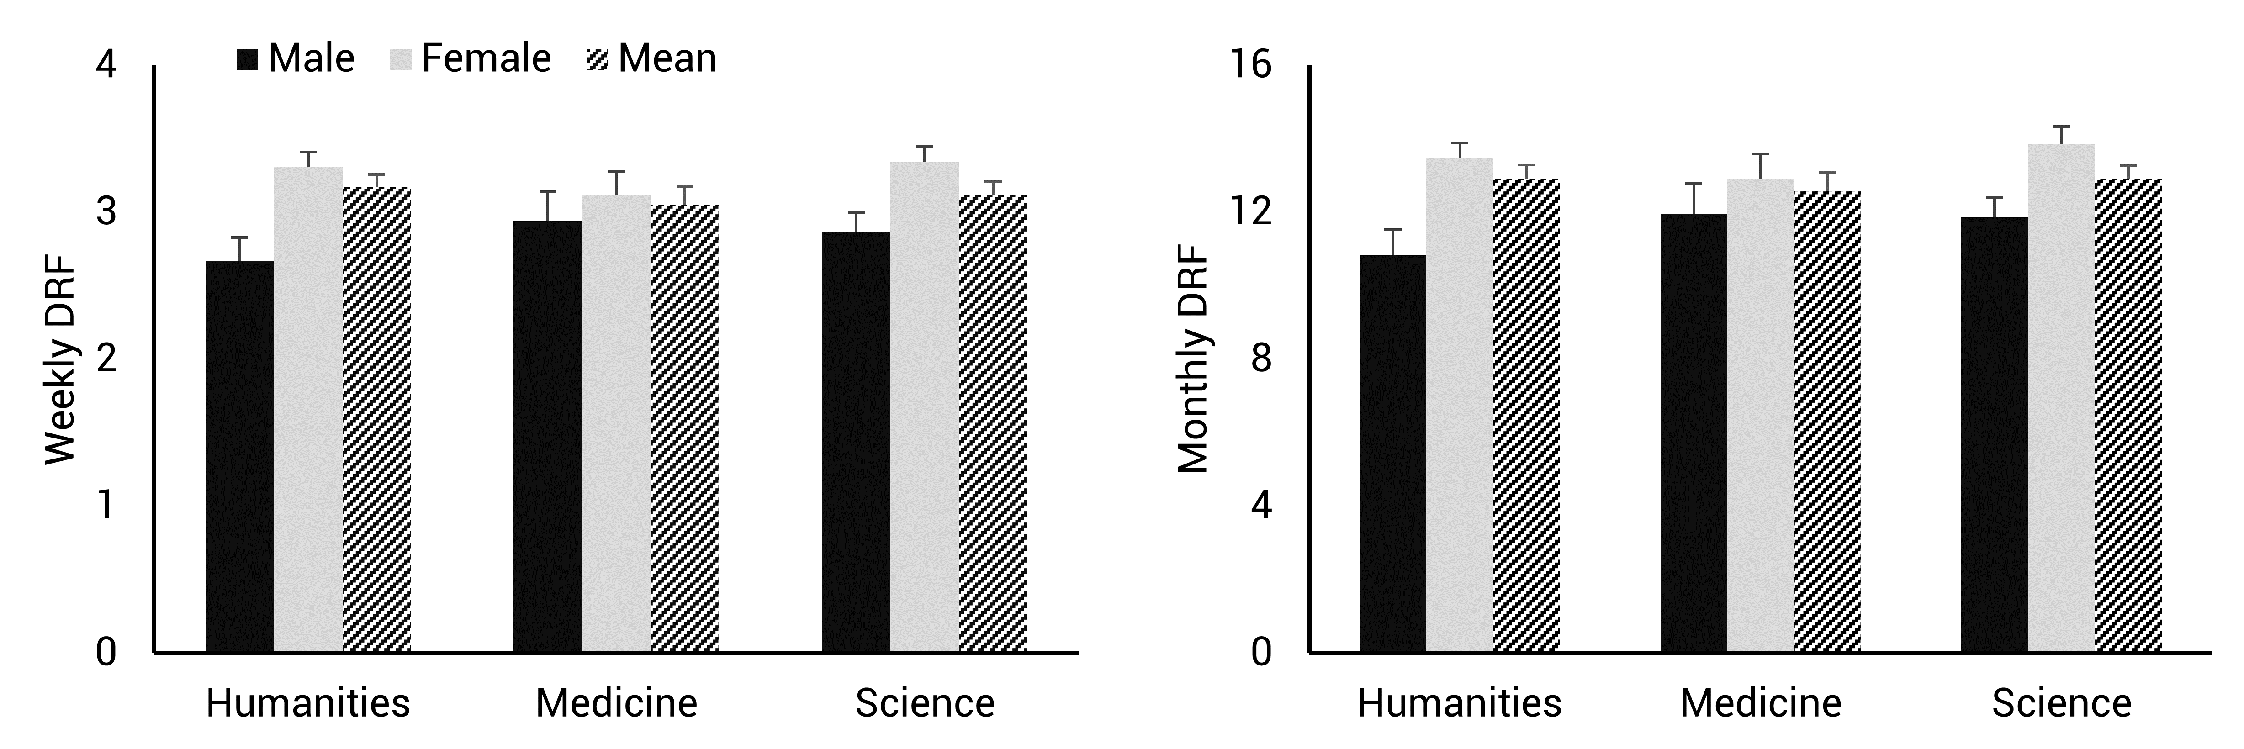
\includegraphics[width=\textwidth]{Fig/Results/Survey/S1_Fig.png}
	\caption*{\textbf{S1 Fig. Dream recall frequency as a function of gender and academic disciplines.} Left: weekly DRF (number of mornings per week with a dream in mind), Right: monthly DRF (number of mornings per month with a dream in mind). Error bars represent standard error.}
\end{figure}

\cleardoublepage

\chapter{Study 5. The relationship between waking life and dream content}
\label{res:wle}

\cleardoublepage

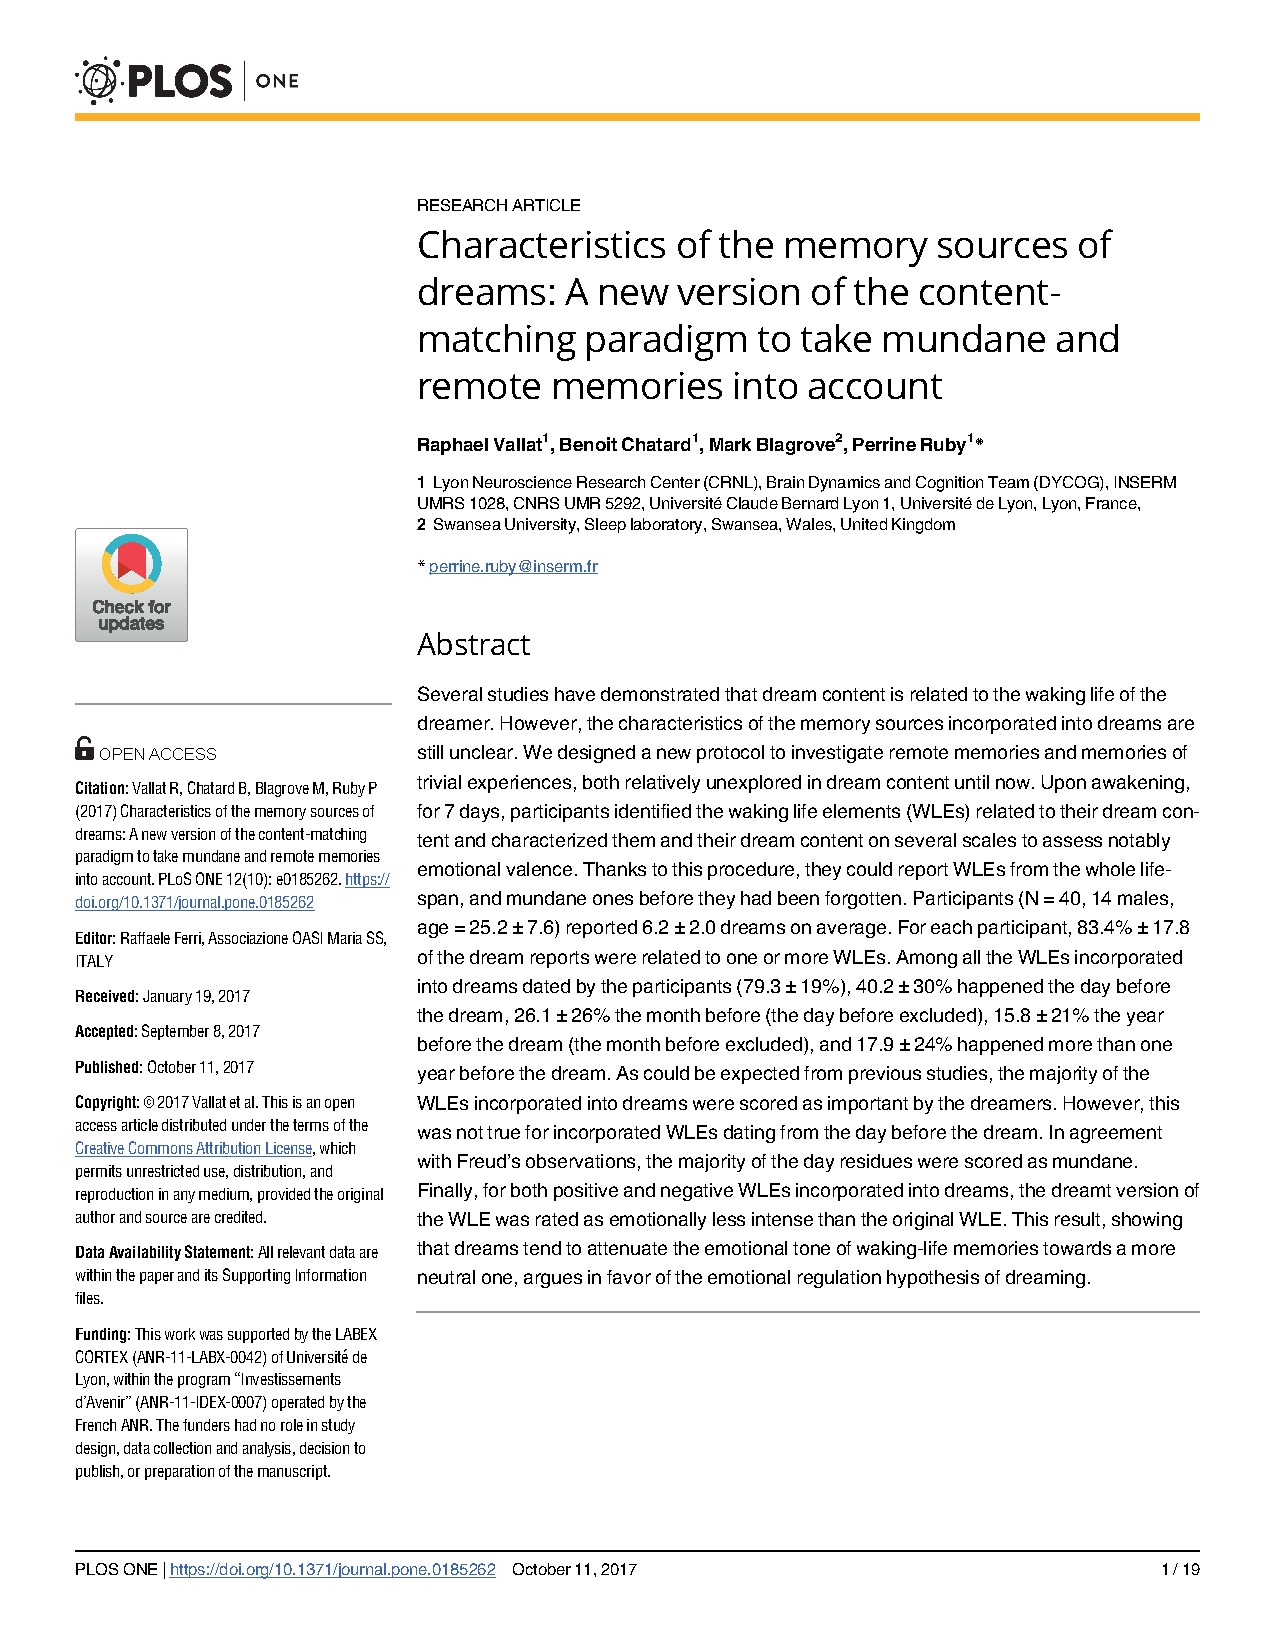
\includepdf[pages=-, pagecommand={\thispagestyle{plain}}]{Articles/Vallat_2017_PlosOne.pdf}

\cleardoublepage

\subsection*{Supplementary materials}
\label{res:wle:supp}
\vspace*{1cm}

\begin{figure}[htbp]
	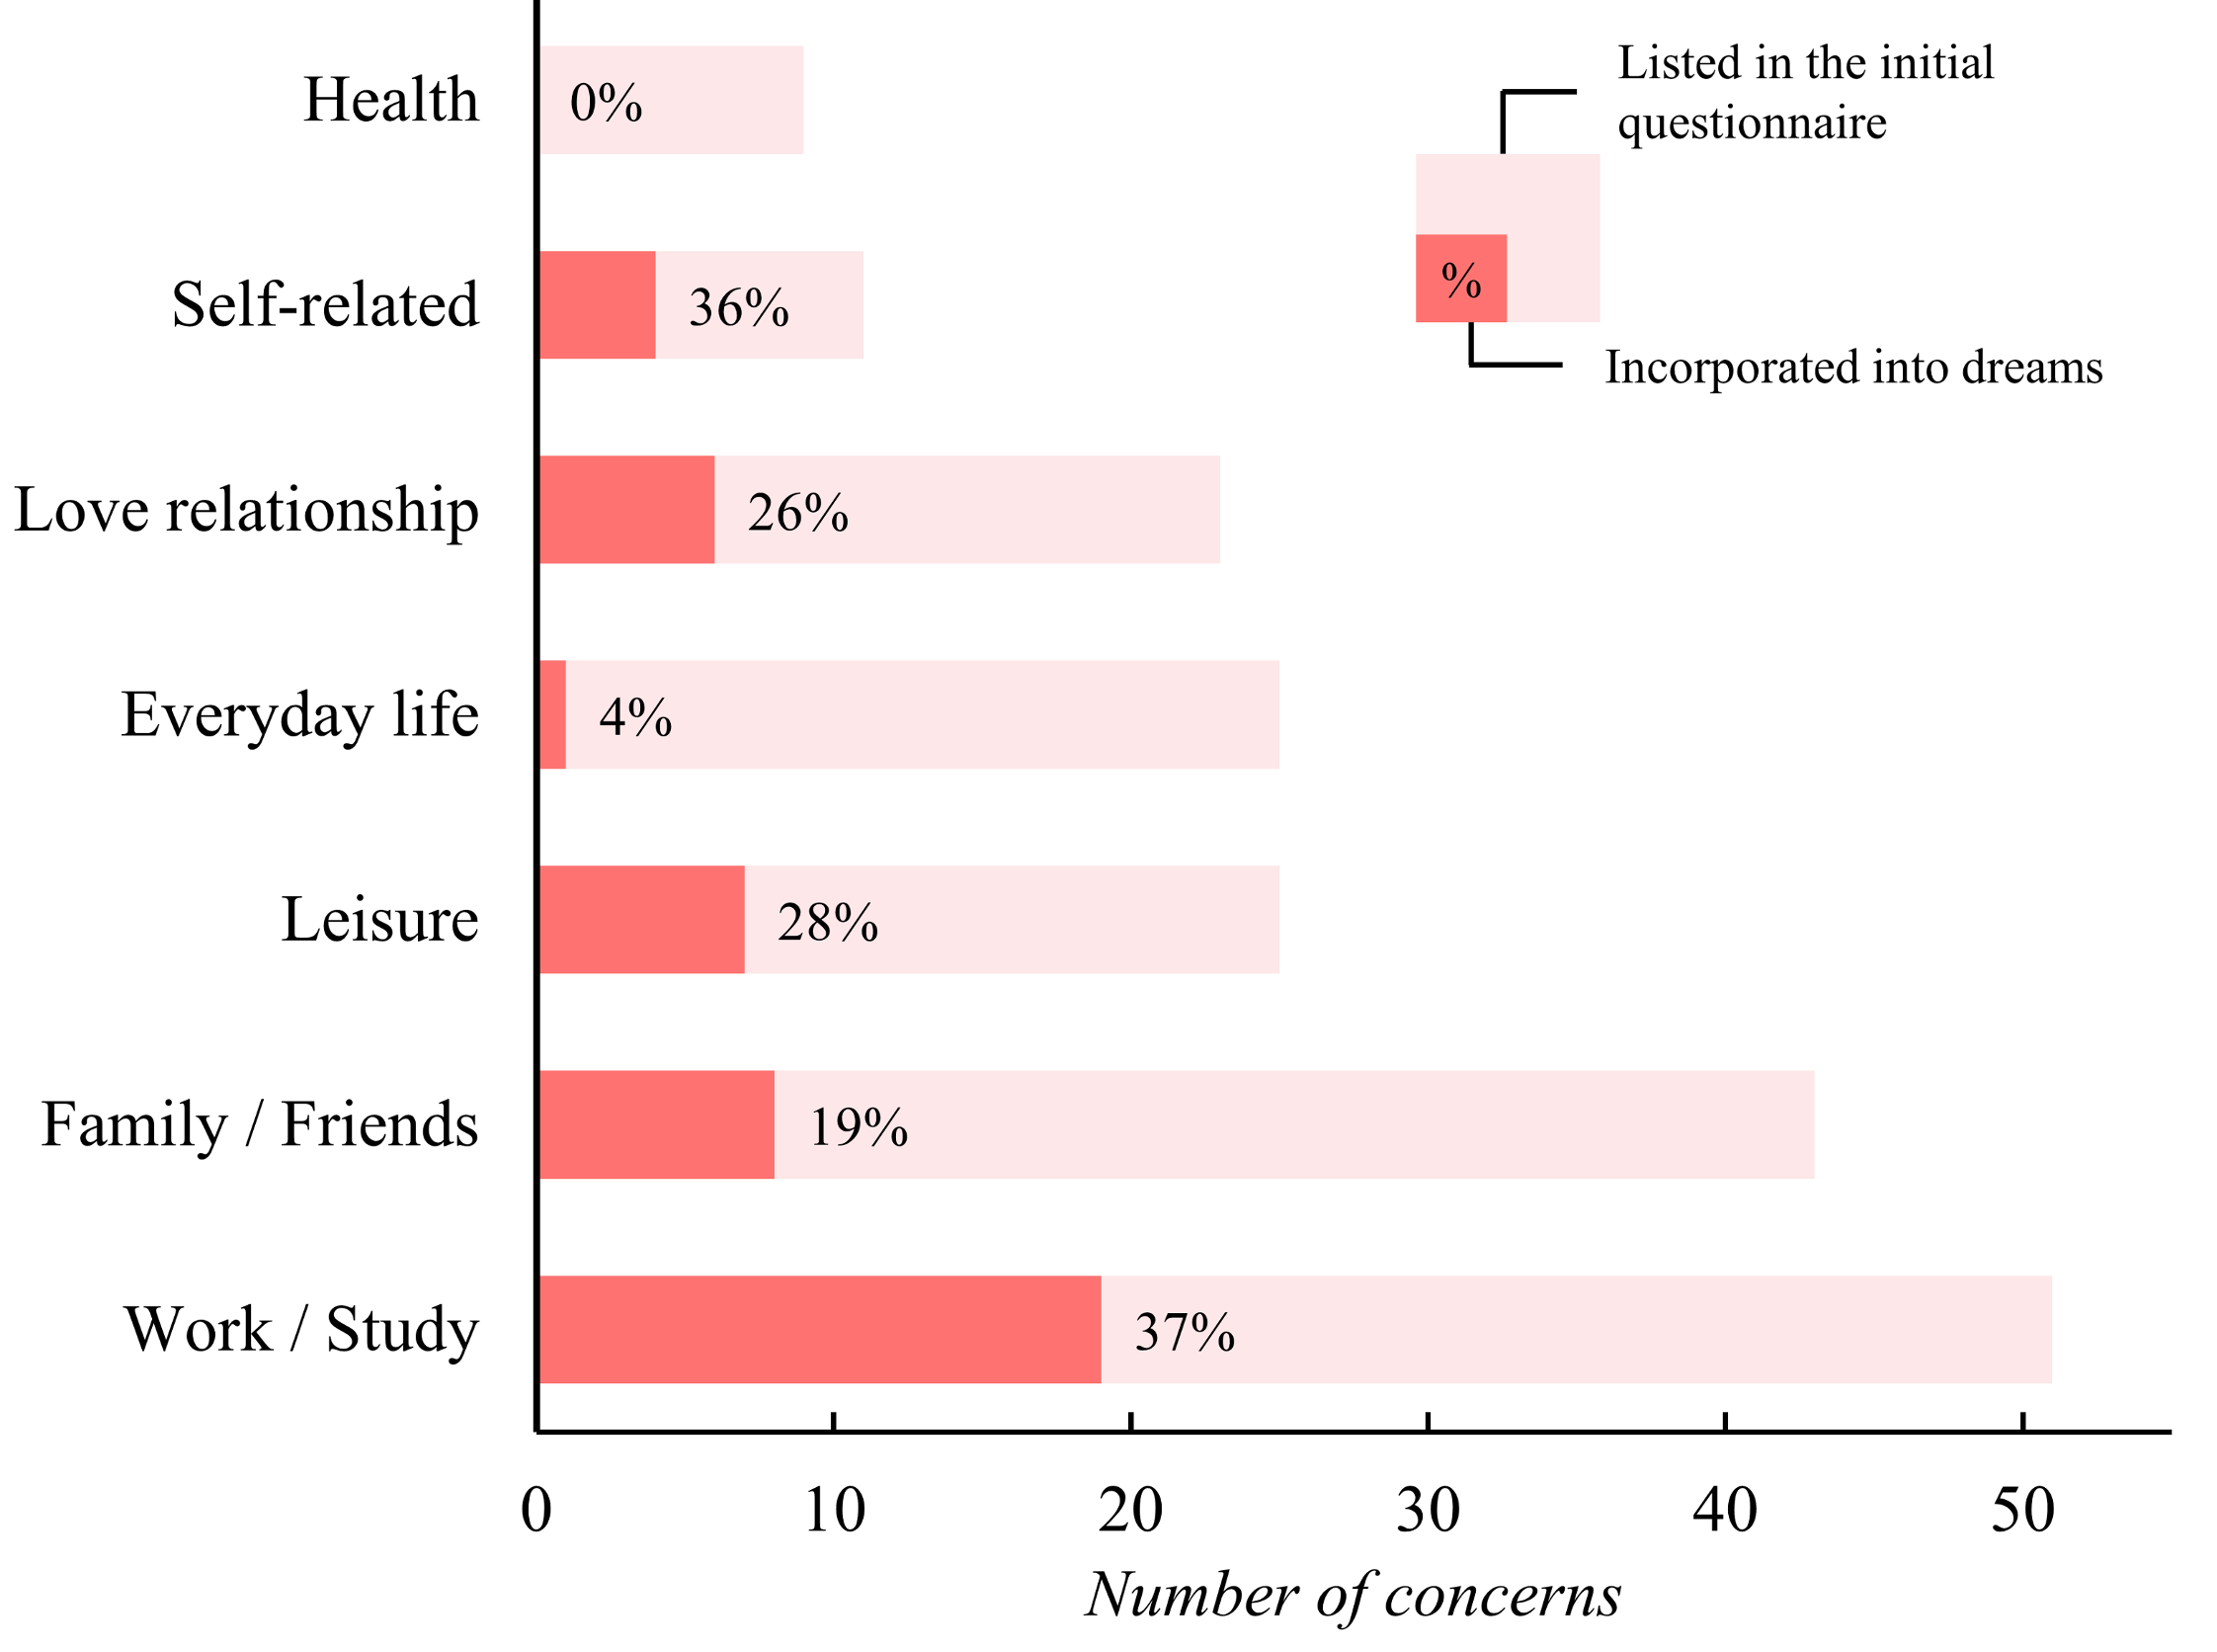
\includegraphics[width=0.72\textwidth]{Fig/Results/WLE/S1_Fig.png}
	\caption*{\textbf{S1 Fig. Concerns reported in the initial questionnaire.} Concerns were distributed in 7 thematic categories. The number of concerns per categories are represented in pink. Red bars illustrate the percentage of concerns from one category that were incorporated into dreams during the 7-days experiment.}
\end{figure}

\vspace*{3cm}

\begin{figure}[htbp]
	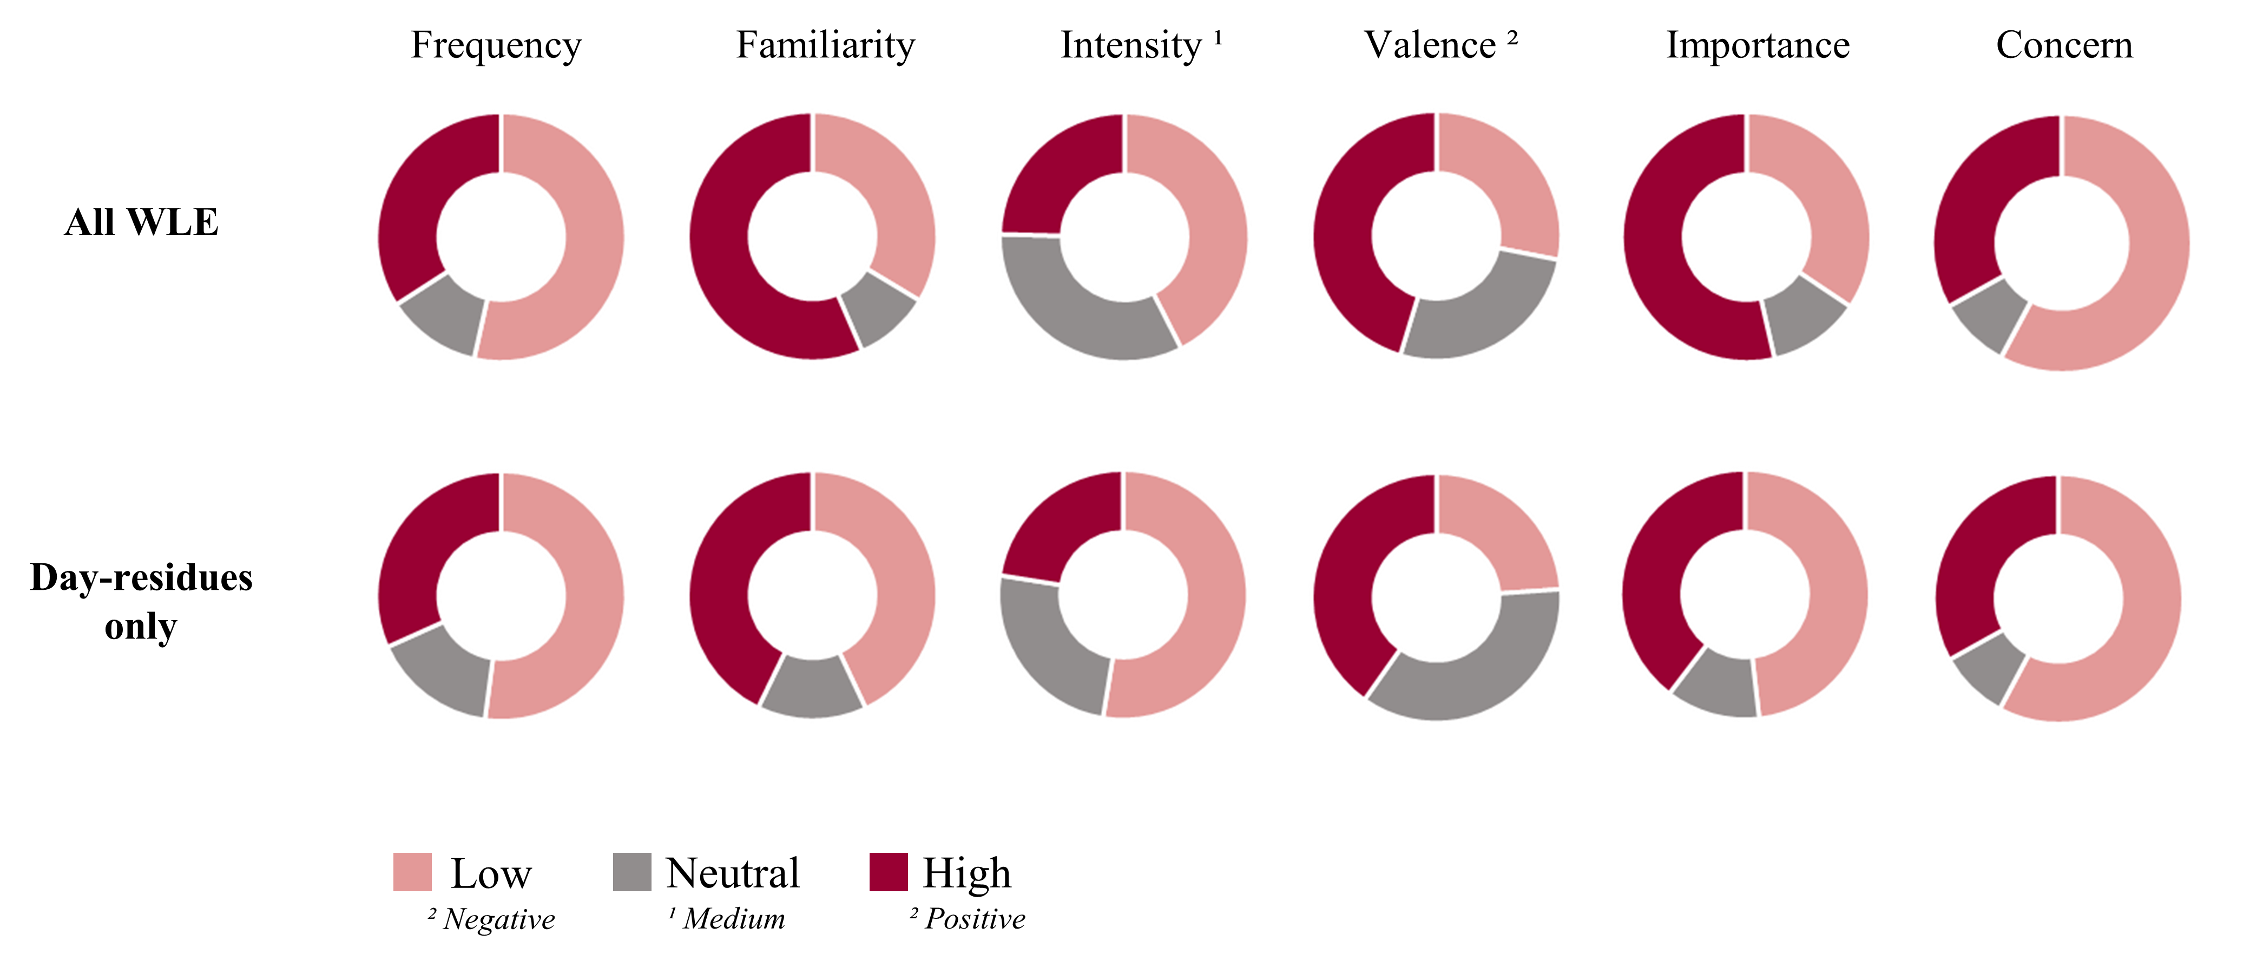
\includegraphics[width=\textwidth]{Fig/Results/WLE/S2_Fig.png}
	\caption*{\textbf{S2 Fig. Distribution of the scores for all the WLEs incorporated into dreams and day-residues only} (see S2 Table for the figures).}
\end{figure}

\FloatBarrier

\clearpage

\textbf{S1 Table. Examples of waking life elements incorporated into dreams.} \\
\noindent\rule{\textwidth}{0.4pt}
\textbf{Old, important and emotionally negative WLE} \\
S1 | Valence = 2 ; Importance = 7 ; Dream valence = 5 \\
Dream report: \q{I am with an ex-girlfriend in my dream, we get along together very well} \\
WLE description: \q{We broke up several years ago in a difficult situation and none of us had given sign of life since.} \smallskip

S29 | Valence = 2 ; Importance = 10 ; Dream valence = 1 \\
Dream report: \q{I descend into another world to pick up my aunt and realize that it is not possible - I feel a deep anguish and I am cold} \\
WLE description: \q{My aunt passed away 3 months ago and I miss her terribly. I know she will not come back, but some days I still hope it will happen.} \smallskip

S35 | Valence = 2 ; Importance = 10 ; Dream valence = 3 \\
Dream report: \q{In my dream I saw my ex-girlfriend and her new partner. Suddenly, I felt really angry and started to push them down the stairs. They fell down and I shout at them.} \\
WLE Description: \q{Three years ago I bumped into them in the streets and was particularly unkind to them.} \smallskip

\textbf{Old, important and emotionally positive WLE} \\
S6 | Valence = 10 ; Importance = 10 ; Dream Valence = 10 \\
Dream report: \q{I was comforting two twins sisters that just got fired from the religious association I was working in several years ago.} \\
WLE description: \q{It reminded me of the responsibility I used to have there.} \smallskip

S19 | Valence = 10 ; Importance = 10 ; Dream Valence = 10 \\
Dream report: \q{I am working at my shop with my employee and my friend F* with whom I get along very well} \\
WLE description: \q{F* is an old school friend. At the time we were always together and for me he was almost part of the family} \smallskip

\textbf{Mundane and feebly emotional day-residues} \\
S3 | Valence = 5 ; Importance = 1 ; Dream valence = 6 \\
Dream report: \q{I was in an unknown house with two friends and a talking Koala.} \\
WLE description: \q{It reminded me of the talking raccoon in the movie Guardian of the Galaxy that I watched the day before.} \smallskip

S15 | Valence = 5 ; Importance = 1 ; Dream valence = 5 \\
Dream report: \q{I am in the supermarket looking for a dishwasher.} \\
WLE description: \q{Yesterday I saw on the internet a picture of the proper way to load dishes in a dishwasher.} \smallskip

S25 | Valence = 5 ; Importance = 1 ; Dream valence = 5 \\
Dream report: \q{In my dream I was creating magical creatures in order to destroy something}. \\
WLE description: \q{The creatures reminded me of the ones in the video game I played for several hours the day before.} \smallskip

S38 | Valence = 5 ; Importance = 1 ; Dream valence = 5 \\
Dream report: \q{I was in a house with a small swimming-pool.} \\
WLE description: \q{The swimming-pool was very similar to the one I saw yesterday in a park. The shape, depth and color were the same.} \smallskip

\textbf{Important and emotionally intense day-residues} \\
S40 | Valence = 1 ; Importance = 10 ; Dream Valence = 1 \\
Dream report: \q{I was at work, struggling to fix several mistakes made by my boss. At the end of the day, I took the blame and got fired.} \\
WLE description: \q{Yesterday there was a problem in my company after a client requested a sudden change.} \smallskip

S33 | Valence = 2 ; Importance = 8 ; Dream Valence = 4 \\
Dream report: \q{My father offers me a sewing machine. I realize that I already have this model.} \\
WLE Description: \q{My father is a recurring concern and we talked yesterday about his health. Also, yesterday I thought that I should sew this week-end.} \smallskip

S29 | Valence = 10 ; Importance = 10 ; Dream Valence = 10 \\
Dream report: \q{I was talking to several persons at the university and each time I tried to say only positive things in order to make them happy.} \\
WLE description: \q{Yesterday I thought that I should really stop being always negative and doubtful. In my dream it felt as if I put into practice this.} \smallskip

S19 | Valence = 10 ; Importance = 10 ; Dream Valence = 10 \\
Dream report: \q{In my dream there was this cartoon character that I really like.} \\
WLE description: \q{Yesterday I watched a really good new cartoon movie.} \\
\noindent\rule{\textwidth}{0.4pt}

\begin{table}[htb]
    \caption*{\textbf{S2 Table. Distribution of the score given to WLEs incorporated into dreams, for all WLEs (bold) and day-residues only.} For emotional valence, Low = negative and High = positive. Emotional intensity is rated on a 1-to-4 scale (see Methods). Neutral = medium emotional intensity.}
    \resizebox{\textwidth}{!}{%
    \begin{tabularx}{\textwidth}{Xlll}
    \toprule
    Characteristics                   & Low (\%)                    & Neutral (\%)          & High (\%)             \\ \midrule
    Frequency (Rare – Daily)          & \textbf{53.5 ± 22.3}        & \textbf{12.4 ± 11.4}  & \textbf{34.2 ± 24.2}  \\
                                      & 52.1 ± 33                   & 16.2 ± 25             & 31.7 ± 35             \\
    Familiarity (New – Familiar)      & \textbf{33.6 ± 21.7}        & \textbf{9.9 ± 14.5}   & \textbf{56.5 ± 23}    \\
                                      & 43 ± 37                     & 14.2 ± 25             & 42.9 ± 37             \\
    Emotional valence (Neg. – Pos.)   & \textbf{28.1 ± 20.9}        & \textbf{26.6 ± 25.3}  & \textbf{45.3 ± 26.2}  \\
                                      & 23.9 ± 28                   & 35.9 ± 34             & 40.2 ± 37             \\
    Importance                        & \textbf{34.4 ± 23.6}        & \textbf{12 ± 12.7}    & \textbf{53.5 ± 22.9}  \\
                                      & 48.2 ± 37                   & 12.2 ± 25             & 39.6 ± 38             \\
    Current concern                   & \textbf{56.6 ± 25.1}        & \textbf{9 ± 13.8}     & \textbf{34.4 ± 21.6}  \\
                                      & 57.8 ± 37                   & 9.1 ± 21              & 33.1 ± 33             \\
    Emotional intensity               & \textbf{42.5 ± 25.4}        & \textbf{32.9 ± 24.4}  & \textbf{24.6 ± 23.4}  \\
                                      & 52.6 ± 38                   & 24.9 ± 32             & 22.5 ± 33             \\ \bottomrule
    \end{tabularx}%
    }
\end{table}

\begin{table}[htb]
    \caption*{\textbf{S3 Table. Characteristics of the WLEs incorporated into dreams that happened 6 to 9 days before the dreams (n=36)}. Except for emotional intensity, Neutral (\%) refers to the percentage of WLEs with a score of 5. For emotional valence, Low = negative and High = positive. Emotional intensity is rated on a 1-to-4 scale (see Methods). Neutral = medium emotional intensity.}
    \resizebox{\textwidth}{!}{%
    \begin{tabularx}{\textwidth}{Xllll}
    \toprule
    Characteristics                 & Mean Score      & Low (\%)  & Neutral (\%) & High (\%) \\ \midrule
    Frequency (Rare – Daily)        & 4.1 ± 2.9       & 49.3 ± 48 & 18.6 ± 37    & 32.1 ± 42 \\
    Familiarity (New – Familiar)    & 5.2 ± 3.0       & 38.1 ± 43 & 25.2 ± 42    & 36.7 ± 42 \\
    Emotional valence (Neg. – Pos.) & 5.4 ± 2.1       & 24.6 ± 36 & 22.5 ± 39    & 52.9 ± 46 \\
    Importance                      & 5.7 ± 3.0       & 21.9 ± 34 & 19.5 ± 31    & 58.6 ± 39 \\
    Current concern                 & 5.1 ± 3.4       & 39.3 ± 40 & 8.6 ± 27     & 52.1 ± 40 \\
    Emotional intensity             & 1.4 ± 1.3       & 56.1 ± 46 & 31.8 ± 41    & 12.1 ± 29 \\ \bottomrule
    \end{tabularx}%
    }
\end{table}

% Table column width
\newcolumntype{b}{>{\hsize=0.35\textwidth}X}

\begin{table}[htb]
    \caption*{\textbf{S4 Table. Distribution (\%) of mundane WLEs incorporated into dreams according to their temporal remoteness.} Each time category mutually excludes the previous ones (e.g. month before excludes day before the dream).}
    \resizebox{\textwidth}{!}{%
    \begin{tabularx}{\textwidth}{bXXXX}
    \toprule
                                                        & Day before & Month before & More than a month & Not dated \\ \midrule
    Importance < 5, n=196                               & 43.4       & 19.9         & 20.4              & 16.3      \\
    Importance = 1, n=96                                & 52.1       & 17.7         & 17.7              & 12.5      \\
    Importance = 1 and emotional intensity = Low, n=70  & 60         & 20           & 8                 & 12        \\ \bottomrule
    \end{tabularx}%
    }
\end{table}

\subsubsection*{Supplementary results: distribution of the scores }
For each characteristic, the percentage of WLEs with a rating inferior, equal and superior to 5 was computed. A visual inspection of S2 Table shows that if we compare the distribution of the scores for all the WLEs incorporated into dreams and day-residues only, the distributions differ for familiarity, importance, and emotional valence and intensity. As compared to all WLEs incorporated into dreams, for day-residues only we observed a greater percentage of WLEs scored as feebly familiar, emotionally neutral, feebly important and feebly emotionally intense (S2 Fig).

\subsubsection*{Supplementary discussion}
\paragraph{The concern-related dimension of WLEs incorporated into the dreams}

According to the dreamers’ scoring, the WLEs incorporated into dreams are not predominantly concern-related (Table 2). This result is coherent with the experimenters’ assessment of the incorporation of current concerns into dreams taking the initial questionnaire into account. We found that in average 23\% of the dream reports of each subjects incorporated a current concern. Reciprocally, on average for each subject only 25\% of the concerns listed in the initial questionnaire were incorporated into a dream report during the 7 days of the experiment. Previous studies reported a larger percentage of dreams in relation with the dreamers’ current concerns. For example, \citet{schwartz_sleep_2002}, who used an automatic analysis of words on 1770 dreams of the first author found that 35\% of the dreams were considered related to current concerns. The great heterogeneity between studies may come from different definitions of the term \emph{concerns} and from different methods (if close friends and family were considered as concerns, the \% of dreams related to concerns would be much higher in our study). Our results show that when listed a priori (i.e. before dreams content analysis), current concerns are not as represented in dreams as would be expected from the dominant hypothesis saying that \q{much of it tends to revolve around a relative handful of personal concerns} \citep{domhoff_studying_2008}.

\paragraph{The characters and places incorporated into the dreams}

At least one external character was reported for nearly all remembered dreams. The mean number of characters per dream was slightly above with the norm (2.6 in \citealp{hall_content_1966}). This results is most likely due to several methodology differences: in Hall \& Van de Castle system, rating was done a posteriori by an external judge, who would consider groups of characters not individually named (e.g. a couple, a group of 3 children) as one character. In our study, the number of characters was assessed by the dreamer and considering each characters of the dreams as one individual. Regarding familiar existing persons (Fig 2) our results even if a little higher, are also coherent with the norm (familiar characters, 45\% in males and 58\% in females in \citealp{hall_content_1966}). However, in our data close family and friends appeared to be more represented than in the normative study (family, 9\% in males, 14\% in females; relatives, 2\% in males, 4\% in females in \citealp{hall_content_1966})

Regarding places, in our study participants reported nearly twice as much places (2.3 ± 1.5) as in the norm (average n° of settings per dream, 1.3 in \citealp{hall_content_1966}) and nearly half of these places were unknown (Fig 2) which is far more than the norm (unfamiliar, 14\% \citealp{hall_content_1966}). Finally, we observed a little less familiar places (familiar, 33\% \citealp{hall_content_1966}) and a little less mixed places (questionable, 40\% \citealp{hall_content_1966}). It is important to keep in mind that in our study the dreamers rated their own dreams while in \citet{hall_content_1966} an external rating was used. The two methods may yield divergent results \citep{sikka_i_2014}.

\cleardoublepage

\chapter{Study 6}
\label{res:software}

\cleardoublepage

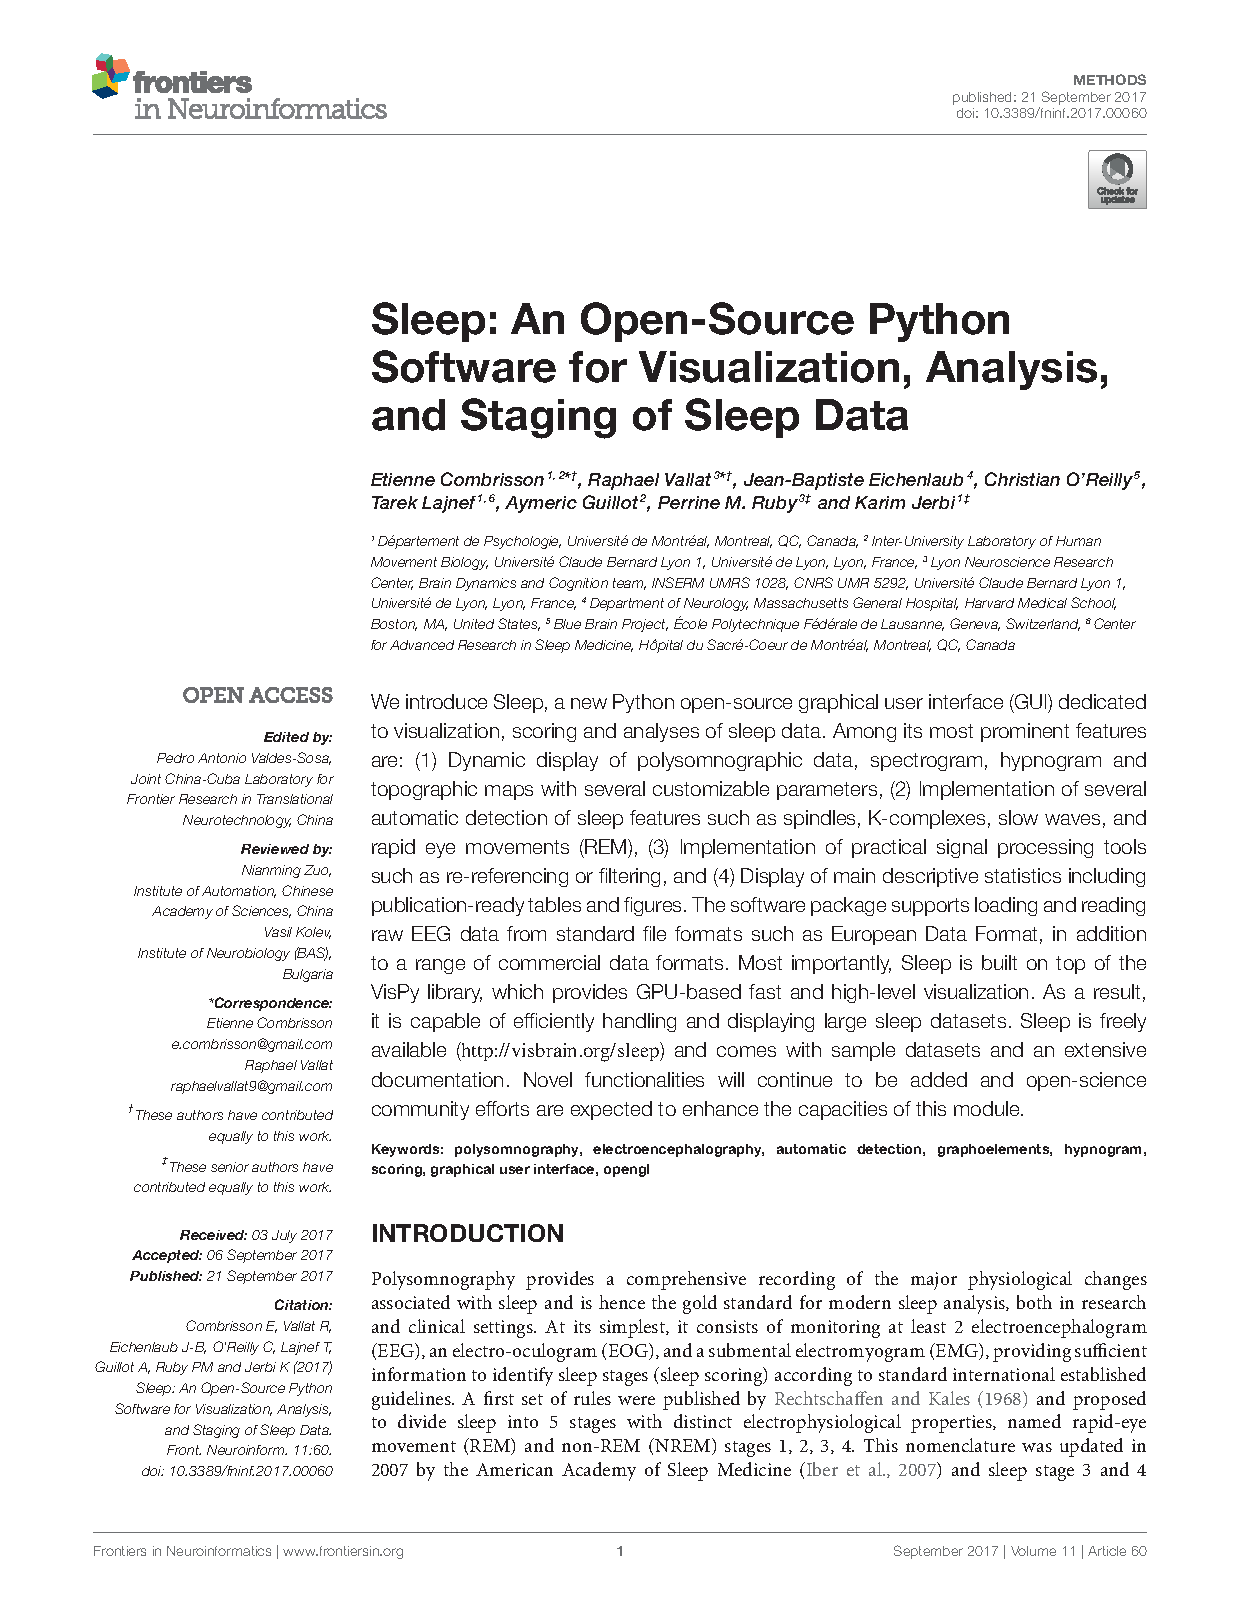
\includepdf[pages=-, pagecommand={\thispagestyle{plain}}]{Articles/Combrisson_2017_FIN.pdf}


\cleardoublepage
\part{GENERAL DISCUSSION}
\cleardoublepage
\chapter{Neurophysiological and behavioral factors associated with a high DRF}
\label{disc:drf}

\section{Summary of the results}
\label{disc:drf:summary}

One of the major objectives of the present thesis was to investigate the neurophysiological and behavioral correlates of inter-individual variability in dream recall frequency (DRF). Based on previous findings, we hypothesized that DRF is associated with a specific psychological and physiological functioning during both sleep and wakefulness. To test this hypothesis, we conducted several experiments to compare the brain activity, sleep parameters, cognitive abilities and personality traits of high and low dream recallers (HR and LR, respectively). The main findings of our experiments are summarized in Fig \ref{fig:disc:drf:summary}.

\begin{figure}[!htb]
	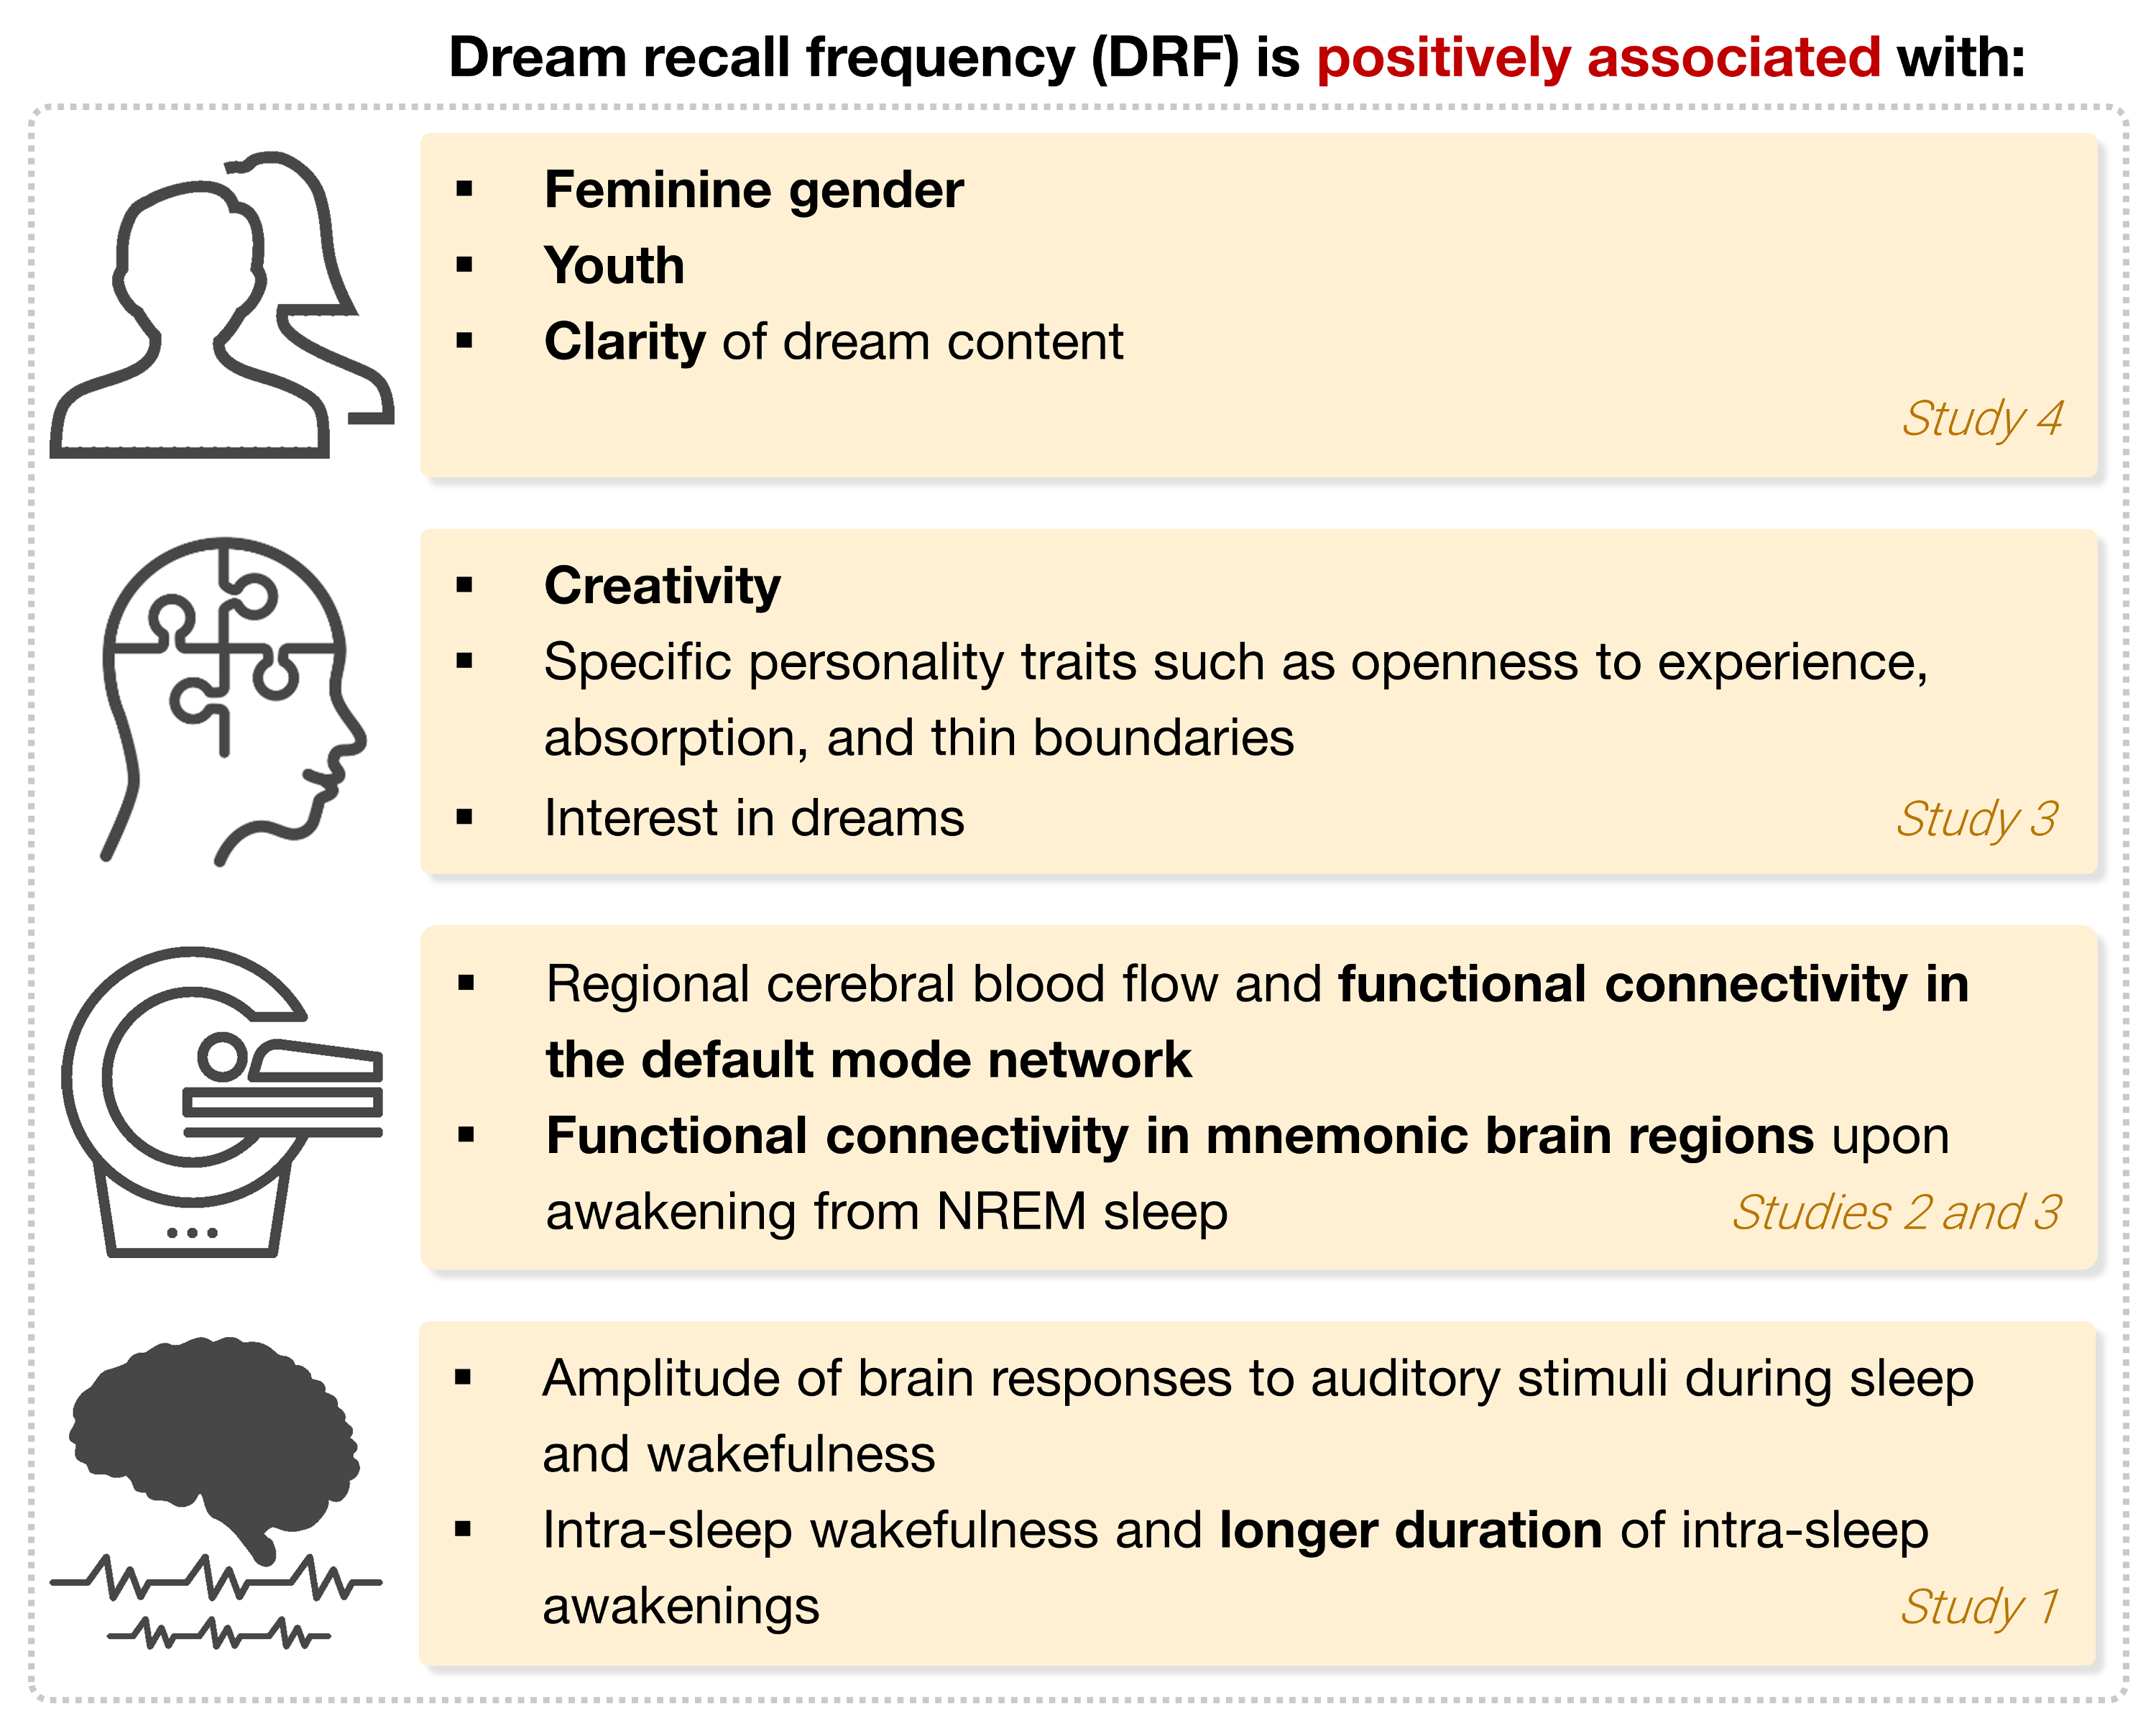
\includegraphics[width=\textwidth]{Fig/Discussion/HR_recap.png}
	\caption[Summary of the results on DRF]{\textbf{Summary of the differences observed between high and low dream recallers}. The findings of the present thesis are written in bold. By opposition, DRF was not associated with memory abilities or the density of certain sleep microstructural events such as rapid eye movements, muscle twitches, spindles and K-complexes.}
	\label{fig:disc:drf:summary}
\end{figure}

\subsection{DRF is positively associated with increased brain reactivity and longer intra-sleep awakening}
\label{disc:drf:summary:arousals}

In Study 1, we performed an in-depth investigation of the sleep macro and micro-structure of HR and LR by re-analyzing the polysomnographic recordings of \citet{eichenlaub_brain_2014}. First, we did not find any significant between-group differences in any of the sleep microstructural features considered (e.g. arousals, spindles, K-complexes, REMs). Our interpretation of these findings is that, most probably, sleep microstructural features are not crucial factors to explain DRF variability.
By contrast, we observed that full awakenings (i.e > 15 seconds) were longer in all sleep stages in HR as compared to LR (roughly 2 vs 1 min respectively). Noteworthy, the number of awakenings was not different between the two groups.

These observations led us to propose that among sleep parameters, the duration of intra-sleep wakefulness seems to be the most critical predictor of inter-individual differences in DRF. This result provides a strong evidence in favor of the arousal-retrieval model (see section \ref{sec:dream-recall:theories:arousal}, \citealp{koulack_dream_1976}), which states that a short period of wakefulness has to occur immediately after dreaming in order to transfer the dream content from short to long term memory. Our findings constitute an important contribution to this model by demonstrating, using objective measurements, a link between intra-sleep awakening and DRF. These results also extended this model by showing that the duration of awakenings is more critical to dream recall than the number of awakenings. We proposed that awakenings must be of sufficient duration to allow successful encoding of dreams into memory. Based on our results and previous ones \citep{campbell_perception_1981}, we suggested that 2 minutes might be the threshold duration for a successful encoding.

On this point, it should be noted that the author of the present thesis contributed to an ongoing study aiming at investigating, by means of human intra-cortical EEG, the temporal dynamic of reactivation of brain regions involved in memory processing during arousals (ranging from 3 sec to 2 minutes). Preliminary results showed that the spectral composition of hippocampal EEG signal during these arousals was intermediate between that of sleep and wakefulness activities in NREM and REM sleep, and that this activation was modulated by the awakening duration (Eskinazi et al., \emph{in preparation}, see \hyperref{sec:publications}{Publications} list). Furthermore, we observed that hippocampus activity during these arousals was different during NREM and REM sleep, a finding particularly relevant considering the well-known dichotomy between these two sleep stages with regards to dream recall and, more broadly, memorization processes \citep{nielsen_review_2000, conduit_poor_2004}.

The visual scoring of arousals allowed us to address another issue, which is related to the finding of differential brain reactivity to auditory stimuli in high and low dream recallers (see section \ref{sec:dream-recall:param:neuro}). \citet{eichenlaub_brain_2014} has suggested that there might be a causal link between the larger brain responses to auditory stimuli and greater intra-sleep wakefulness during sleep in HR as compared to LR. In other words, the amplitude of brain responses to auditory stimuli could be predictive of subsequent awakening or arousal reactions, an observation that has been previously reported for nociceptive stimuli \citet{bastuji_laser_2008}. To test this hypothesis, we computed the auditory evoked potentials to arousing stimuli (i.e. inducing either an arousal or awakening within the next 15 sec) or non-arousing stimuli (i.e. stimuli that do not induce a disruption of the PSG signal within the next 15 sec). This comparison was not possible without the tedious and time-consuming visual scoring of arousals, given that arousals are far more frequent than awakenings in a normal night of sleep, and are therefore needed to compute reliable and statistically valid evoked potentials. Consistent with our hypothesis, we have shown that brain responses to auditory stimuli, in N2 sleep, were larger when followed by a subsequent arousing reaction. Importantly, this increase in the amplitude of the brain responses seemed to be truly related to the stimulus since the amplitude was larger when arousing reactions were within 5 seconds after the stimulus compared to when they were between 5 and 15 seconds. Although it was not possible to compare the brain responses to arousing stimuli between HR and LR (because of too few subjects in each group having a sufficient number of arousing stimuli), behavioral results showed that HR elicited a significantly greater proportion of arousing reaction than LR, thus confirming the idea of a greater brain reactivity to external stimuli in HR \citep{eichenlaub_brain_2014}.

In sum, our findings argue for the existence of a causal link between intra-sleep awakening and the brain reactivity to stimuli during sleep. As compared to LR, a greater brain reactivity during sleep in HR could promote intra-sleep awakening which could in turn promote dream recall. Our hypothesis is that if these awakenings are of sufficient duration to allow for the reactivation of the memory encoding abilities of the brain (and notably the hippocampus), then the dream content can be successfully encoded into long-term memory and therefore successfully recalled in the morning. That said, it should be taken into account, however, that DRF variability is unlikely to be explained fully through this one mechanism, since studies have shown that even when awakened at specific moment during the night and under controlled laboratory condition, LR still report significantly less dreams than HR (\citealp{goodenough_comparison_1959}, also replicated in Study 2 of this thesis). Consequently, it is reasonable to assume that some other factors mediate the forgetting and recalling of dreams. A factor that has been proposed but surprisingly never experimentally tested until now is the brain and cognitive functioning during the transition from sleep to wakefulness (i.e. sleep inertia).

\subsection{DRF is positively associated with brain functional connectivity upon awakening}
\label{disc:drf:summary:inertia}

In Study 2, we tested the hypothesis of a differential sleep inertia between HR and LR. To this aim, we designed an EEG-fMRI sleep study to compare specifically the brain functional connectivity and cognitive performances of these two groups following awakening from a daytime nap. To our knowledge, this was the first study to experimentally test the relationship between sleep inertia and DRF. Our predictions were that HR would show less cognitive impairments and brain functional alterations than LR at awakening, therefore allowing them to better encode dream content upon awakening from sleep.

While we were not able to evidence significant behavioral between-group differences at awakening (discussed in section \ref{res:inertia:drf:discussion}), our results showed on a differential brain functional organization associated with DRF in the minutes following awakening from sleep. We found that at 5 min-post-awakening, HR exhibited a greater functional connectivity within the default mode network and regions involved in memory retrieval, such as the medial prefrontal cortex (MPFC), the precuneus, the left medial temporal lobe (MTL) and the left dorsolateral prefrontal cortex (DLPFC). Remarkably, these are almost exactly the same regions found to be involved in episodic memory encoding and retrieval (reviewed in \citealp{spaniol_event-related_2009}). Our interpretation of these results is that the higher functional connectivity in mnemonic brain regions observed in HR could facilitate in these participants the retrieval of dream content, by preventing the loss of the short-term dream memory during the sleep-wake transition. Inversely, LR could fail to recall their dreams because of greater functional connectivity alterations during the first minutes following awakening. More broadly, our results argue in favor of a differential functional awakening process between HR and LR that could explain inter-group differences in dream recall.

On another topic, it is important to note that this study was also the first to investigate simultaneously the brain and cognitive alterations of sleep inertia in healthy subjects (\hyperref{res:inertia:inertia}{part 1 of Study 2}). Using measures of arithmetic performances at pre-sleep, 5 min and 25 min post-awakening, we replicated the finding of reduced cognitive performances just after awakening as compared to before sleep or 25 min after awakening. Furthermore, we provided a brain mechanism for these cognitive impairments, by showing a global loss of brain functional \emph{segregation} following awakening from N2 and N3 sleep. Consistent with the well-known link between the severity of sleep inertia and the prior sleep stage \citep{tassi_sleep_2000}, we found that awakening from N3 sleep was associated with the most severe and robust changes in the brain functional connectivity. Among the perspectives for future studies, it would be interesting to extend these data to N1 sleep and REM sleep, which are known to induce less sleep inertia than N2 or N3 sleep. However, REM sleep is very difficult to observe in an MRI setting, unless applying a severe and specific REM sleep deprivation in the night(s) before \citep{duyn_eeg-fmri_2012}, which is of course not ideal to study functional connectivity given the huge impact of severe sleep deprivation on the brain functional connectome \citep{de_havas_sleep_2012, yeo_functional_2015, krause_sleep-deprived_2017}.

\subsection{DRF is positively associated with creative-thinking abilities and default mode network connectivity}
\label{disc:drf:summary:dmn}

There is a rising consensus that dreaming, or at least dream recall, could be subserved by regions of the default mode network (DMN). In Study 3, we re-analyzed the fMRI data of Study 2 to specifically investigate the relationship between DRF and the DMN. Our results show that, during rest and compared to LR, HR exhibit a higher functional connectivity within the DMN (1) in average and (2) specifically between the MPFC and TPJ. These results are remarkably consistent with previous ones showing a higher rCBF in HR between these two same regions during sleep and wakefulness \citep{eichenlaub_resting_2014}, and a cessation of dream reporting following focal lesions in these brain areas \citep{solms_neuropsychology_1997}. Based on all these observations, one can reasonably argue that the TPJ and the MPFC are two critical regions when it comes to the ability to recall dreams. The question remains yet pending whether these regions are only involved in dream recall during wakefulness, or also in the production of dreams during sleep. It would be premature to answer that question given that we still have no other means than awakening the participants to assess whether he or she was dreaming.

The second goal of this study was to compare the cognitive abilities (e.g. memory, creativity) and personality traits of HR and LR. We found that HR scored higher than LR on measures of creative-idea generation, without any further between group differences in memory or cognitive abilities. Regarding personality traits, we found that HR tended to score higher on several big five dimensions such as neuroticism, agreeableness and openness-to-experience. These differences were however not significant. This could be due, in part, to the number of participants (n=55), which despite being great for a typical neuroimaging study (especially involving simultaneous EEG-fMRI recordings), is rather low for behaviorally assessing subtle differences in personality traits (e.g. n=981 in \citealp{hartmann_boundaries_1989}). The finding of a higher creativity in HR than in LR, which has already been reported in several studies \citep{fitch_variations_1989, schredl_creativity_1995, schredl_factors_2003}, is particularly interesting given that creative-thinking has also been associated with the recruitment of the DMN \citep{ellamil_evaluative_2012, jung_structure_2013, beaty_creativity_2014, mok_interplay_2014, beaty_default_2015, christoff_mind-wandering_2016}. As such, these findings are consistent with the emerging view that creative-thinking and dreaming share some phenomenological and neurophysiological properties \citep{christoff_mind-wandering_2016}.

Altogether, these results argue in favor of Schonbar's claim \citeyearpar{schonbar_differential_1965} that high or low DRF can be explained by the \q{life-style} of individuals (among which are creative-thinking abilities and personality traits). Our findings go one step further by suggesting that this life-style is related to a specific brain functioning, characterized notably by an increased functional connectivity in the DMN. As we will discuss in section \ref{disc:drf:model}, the question remains to whether there is a causal link between all these variables, and notably whether personality traits, life-style and DRF variations can significantly influence and modify the brain functional properties (and reciprocally).

\subsection{DRF is associated with age, gender, and clarity of dream content}
\label{disc:drf:summary:survey}

We took advantage of the recruitment questionnaire of the EEG-fMRI study on sleep inertia to perform an epidemiological survey of the sleep and dream habits of a large sample of French college students from Lyon University. The survey included several questions regarding DRF. Remarkably, we were able to evidence a negative correlation between DRF and age, even on the tight age range of our sample (i.e. from 18 to 30 years old), as well as a positive correlation between DRF and the clarity of dreams. Furthermore, we were able to replicate the finding of a higher DRF in women than in men \citep{schredl_gender_2008}. Many factors could explain, at least partly, this gender difference in DRF. For instance, \citet{schredl_gender_2008} proposed that it was the result of a gender-specific dream socialization process during childhood. According to them, girls are encouraged more often than boys to talk about their dreams during their childhood, and might therefore develop a stronger interest in dreams, a factor consistently reported to be positively associated with DRF \citep{schredl_factors_2003}. Another possible explanation could be the higher proportion of intra-sleep wakefulness reported in women as compared to men \citep{reyner_gender-and_1995}, which could give them more opportunities to encode dreams into memory according to the arousal retrieval-model \citep{koulack_dream_1976}. Finally, drawing from Schonbar's life-style hypothesis \citeyearpar{schonbar_differential_1965}, one can argue that the higher DRF in women could be the result of differential personality and cognitive traits between men and women. This observation is supported by studies showing higher levels of neuroticism, extraversion, agreeableness, and conscientiousness in women compared to men, as well as a tendency for higher creativity (reviewed in \citealp{schmitt_why_2009, baer_gender_2008}).

Remarkably, age, gender and clarity can all be related to a specific functioning of the default mode network (DMN). For instance, women tend to exhibit a higher functional connectivity in the DMN \citep{bluhm_default_2008}. Similarly, in comparison with younger subjects, older people were consistently found to exhibit a global lower functional connectivity within the DMN \citep{damoiseaux_reduced_2008, koch_effects_2010}, a finding well in line with the observation of reduced mind-wandering abilities in older people \citep{jackson_mind-wandering_2012}. Finally, there is a rising consensus that DMN may be involved in visual imagery process \citep{andrews-hanna_functional-anatomic_2010}, thus suggesting that a high DMN activity could be causally linked to an increased clarity of the dream content. By extension, this could mean that DMN activity is directly related to the salience of dream content. We will discuss further these interactions between DMN functioning and other factors related to DRF in the next section, in which we propose an integrative model of dream recall based on all these findings.

\section{An integrative model of dream recall}
\label{disc:drf:model}

How can we combine the above findings on DRF variability to the previously existing knowledge on dream recall?
The results of the present thesis led us to propose a comprehensive and integrative model of dream recall, depicted in Fig \ref{fig:disc:drf:model}.

The main assumption of this model is that successful dream recall requires the encoding, during the sleep-wake transition, of the dream short-term memory into a more stable long-term memory. As proposed by \citet{koulack_dream_1976} and since then confirmed in numerous studies, this process is not possible during sleep but only during wakefulness. Consistent with this, we reported earlier that DRF is positively associated with intra-sleep wakefulness, and notably with the duration of awakenings. This observation led us to propose that intra-sleep awakenings must be of sufficient duration to allow the reactivation of the memory encoding abilities of the brain. Apart from the duration, other factors come into play to either facilitate or prevent the encoding of dreams during the period following awakening from sleep.

First, state-factors such as sleep inertia, and the magnitude of the functional difference between the pre- and post-awakening brain state \citep{koukkou_dreaming:_1983} are negatively associated with successful encoding of dream content. Both these factors are related to the physiological context, which include notably the prior sleep stage and sleep duration, the level of sleep deprivation and the time of the night (i.e. circadian factor). Second, as proposed by \citet{cohen_dream_1973}, the dream memory trace remains so long as there is no distraction or interferences in the encoding process. According to our model, the level of interferences could be directly related to traits factors, such as the interest in dreams. For instance, individuals highly interested in their dreams will probably make a voluntarily effort to \emph{grasp} the dream memory, and at the same time avoid interferences in the encoding process. This relationship could explain why DRF is known to be significantly enhanced by keeping a dream diary \citep{schredl_questionnaires_2002}. This could also suggest differential attentional processes between HR and LR. This hypothesis was recently tested in an EEG study in which the author of the present thesis contributed (Ruby et al., \emph{in preparation}, see \hyperref{sec:publications}{Publications} list). Consistent with this hypothesis, preliminary findings showed an increase of both top-down and bottom-up attentional processes in HR and LR, thus reinforcing the idea of a differential brain functioning between the two groups.

Another factor that, according to our model, plays a crucial role is the salience of the dream content. This idea first proposed by \citet{cohen_test_1974} and received further support from experimental studies since then \citep{cipolli_bizarreness_1993, schredl_emotions_1998}. Put it simply, this hypothesis states that the more salient a dream is (e.g. vivid, bizarre, emotionally intense), the more likely it will be recalled. This is well in line with the previously mentioned correlation between DRF and clarity of dream content. Furthermore, our model incorporates Schonbar's life-style hypothesis \citeyearpar{schonbar_differential_1965} to postulate that all these processes (e.g. salience, interference, sleep inertia) are influenced by the life-style, personality traits and cognitive abilities (e.g. creativity) of the dreamer.

One of the key finding of the present thesis is that these differential cognitive and personality profiles between high and low dream recallers are also associated with a specific brain functional organization, characterized notably by a higher DMN activity in high dream recallers. According to our model, this specific neurophysiological profile could promote in HR some cognitive abilities such as creativity, which would in turn increase the salience of dream content and promote intra-sleep awakenings. These two factors, associated in HR with reduced brain functional alterations and interferences upon awakening, could facilitate the encoding of dreams and result in an increased dream recall frequency. Lastly, some studies indicate that (1) women score higher on certain personality traits and exhibit a higher DMN functional connectivity (2) aging is negatively associated with cognitive functioning and DMN activity. For these reasons, we believe that age and sex influence, at the lower level, all the following factors related to the process of dream recall.

\begin{figure}[!htbp]
	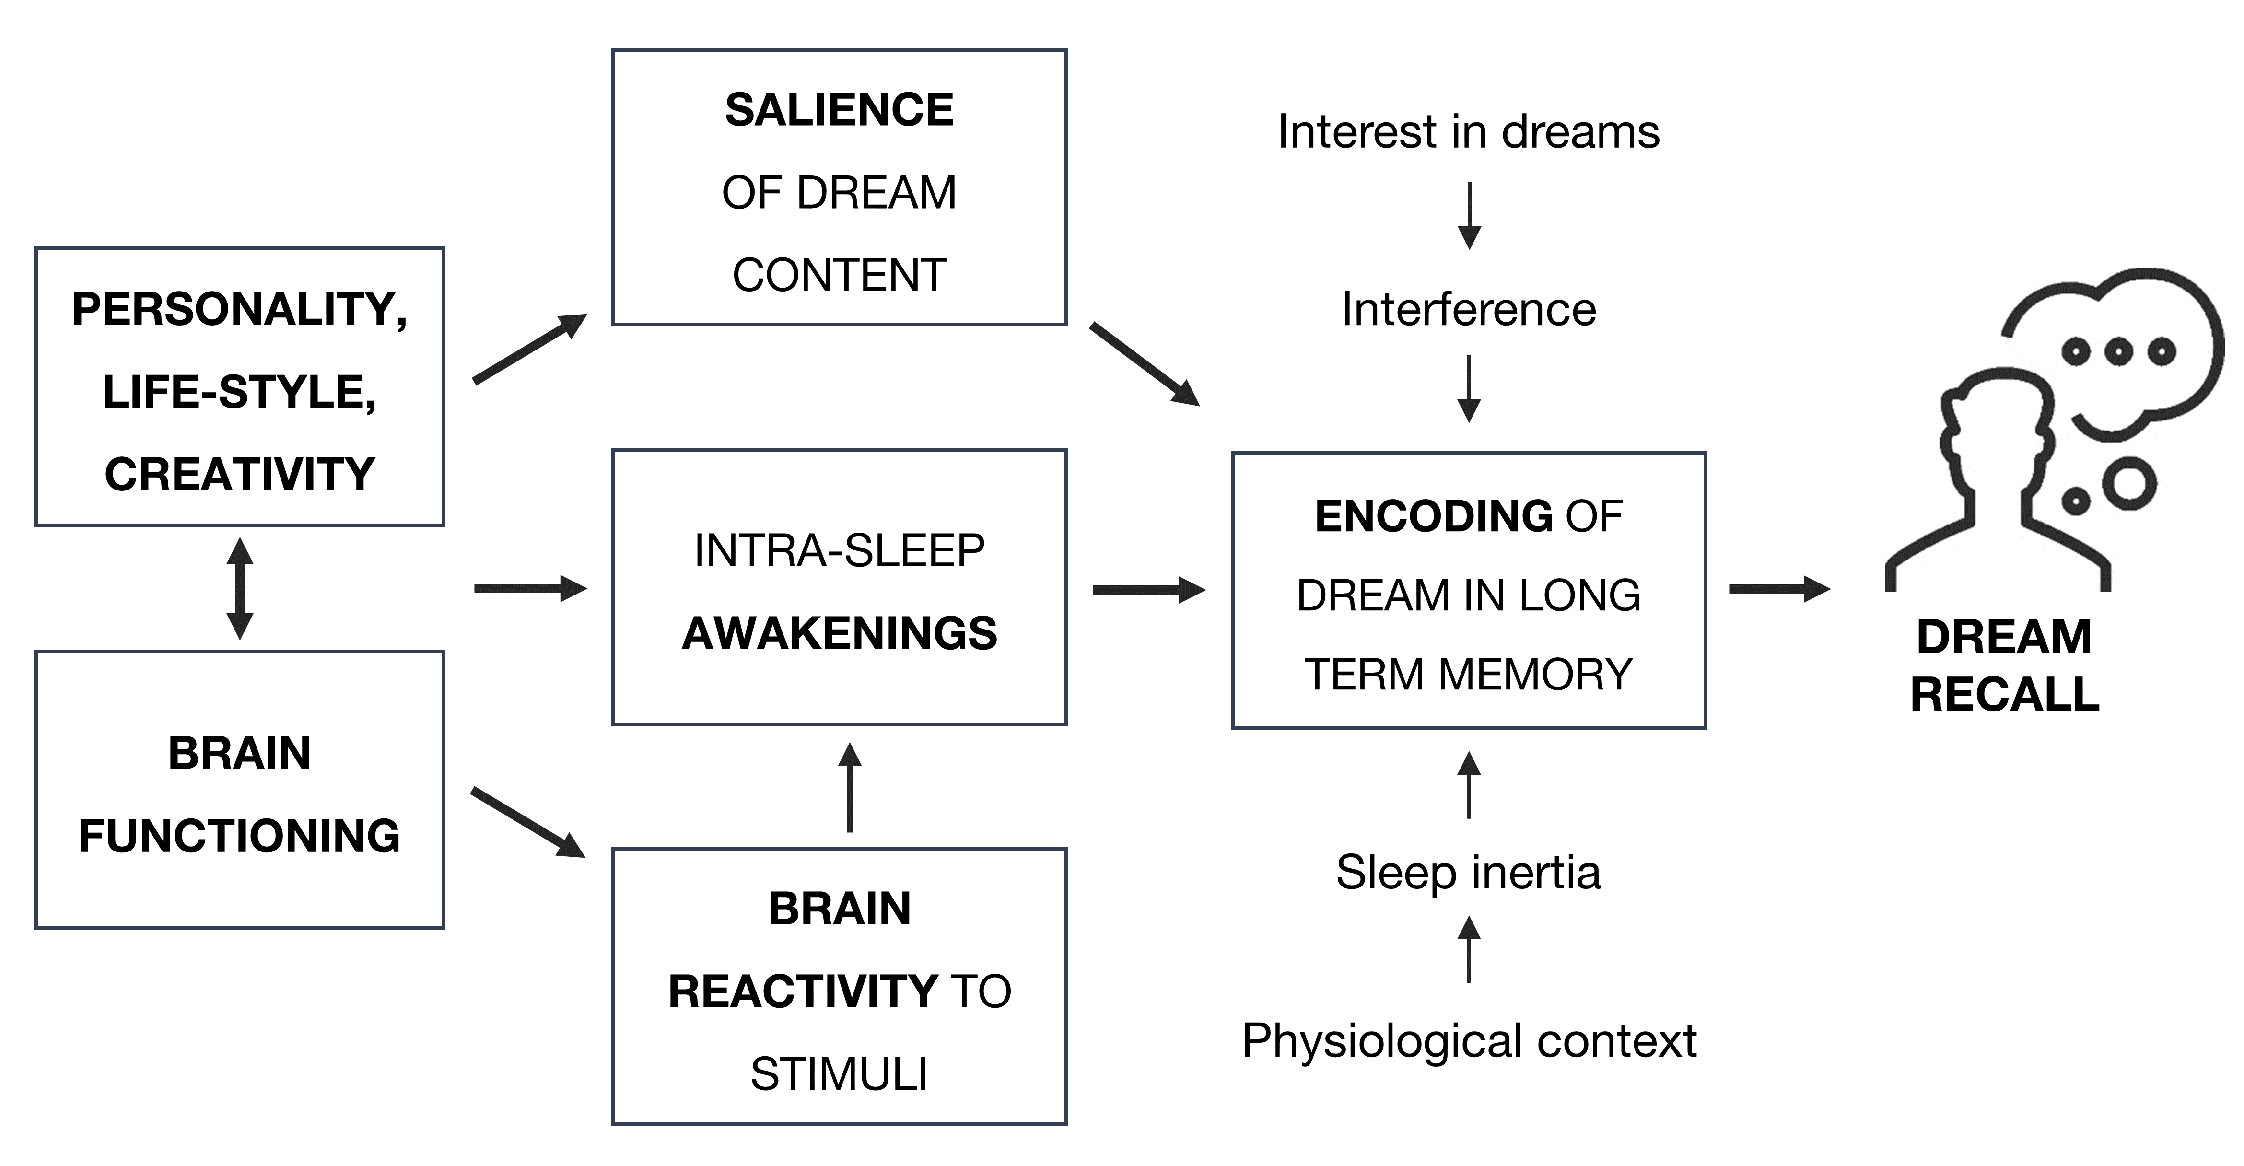
\includegraphics[width=\textwidth]{Fig/Discussion/schema_dream_recall.png}
	\caption[An integrative model of dream recall]{An integrative model of dream recall.}
	\label{fig:disc:drf:model}
\end{figure}

\section{Conclusions and perspectives}
\label{disc:drf:perspectives}

In summary, the different studies of the present thesis significantly improved our knowledge of the factors and their interactions contributing to the process of dream recall. Based on the latests experimental findings, we proposed an integrative model of dream recall which can serve as a basis for future work. Among possible future axes of research, it seems promising to test whether DMN activity could also predict intra-individual variability in DRF across time. To this aim, one could use DRF enhancing methods (such as keeping a dream diary; \citealp{schredl_questionnaires_2002}) to test whether an increased DRF would result in increased creativity scores and DMN functional connectivity in post compared to pre-training measures within the same individuals (preferentially an initial group of low dream recallers).

%%%%%%%%%%%%%%%%%%%%%%%%%%%%%%%%%%%%%%%%%%%%%%%%%%%%%%%%%%%%%%%%%%%%%%%%%%%%%%%
\cleardoublepage
\chapter{The relationship between waking life and dream content}
\label{disc:wle}

\section{Such stuff as dreams are made on}
\label{disc:drf:summary:residue}

\myepigraph{We are such stuff,\\ As dreams are made on; and our little life, \\ Is rounded with a sleep}{William Shakespeare}{The Tempest. 1611}

Through an extensive investigation of the relationship between waking-life and dream content, Study 5 significantly improved our knowledge of the \emph{stuff that dreams are made on}. We asked participants to record and describe, over a period of one week, the obvious connections that they could make between their waking-life and dream content. By specifically investigating the characteristics of waking-life experiences (WLE) incorporated into dreams, we enhanced our understanding of the filter that dreaming applies to waking life.

We observed that the \q{dream mixture}, as Freud called it, is composed of several types of WLE which are all incorporated in significant proportions, i.e. recent and old, emotionally loaded and emotionless, positive and negative, important and insignificant, concerns and non-concern issues, to name but a few. Remarkably, we also found a significant interaction between the temporal remoteness of WLE and their emotional intensity. Older memories were scored by the subjects as the most emotionally intense and important, by opposition with memories of the day before (i.e. day-residues) that were mainly self-rated as non-important and emotionally neutral. However, it should be noted that this effect could be partly explained by the generally low-frequency of emotionally intense WLE. Indeed, none of the participants experienced a highly emotional experience during the 7 days of the experiment. Taken together, the observations of this study led us to support \citet{payne_sleep_2004}'s claim that dream content reflects certain memory processes taking place during sleep. Notably, the selective consolidation and/or forgetting of new memories during sleep (i.e. \q{memory triage}, \citealp{stickgold_sleep-dependent_2013}) could be function of the adaptive relevance and the emotional intensity of these memories \citep{schwartz_are_2003, malinowski_memory_2014, saletin_role_2011}.

\section{A role of dreaming in emotional regulation}
\label{disc:drf:summary:regulation}

The questionnaires that the participants had to fill in each morning after awakening included questions regarding the emotional tone of the waking-life memories, not only as they were experienced originally, but also as they were experienced within the dream content. Remarkably, we found that the dreamed version of the WLE was emotionally down-regulated compared to its waking-life counterpart form. Both emotionally positive and negative WLE were rated as less emotionally intense within dreams as compared to their original occurrence in waking-life.

These results suggest the existence of a down-regulation of emotional waking memories during dreaming (i.e. attenuation of the emotional intensity of waking memories toward a more neutral tone), and provide as such one of the very few experimental evidences supporting the emotional regulation theory of dreaming \citep{cartwright_role_1998, cartwright_role_1998-1, perogamvros_roles_2012}, which claims that dreaming may actively moderate mood overnight in healthy individuals (see section \ref{sec:dream-func:modern:emotion}). Taking up the idea of dreams as an open-window on the cognitive processes occurring during sleep, this down-regulation of emotional waking memories observed in dream content could be the result of an overnight modulation of affective neural system and reprocessing of emotional experiences \citep{walker_overnight_2009, goldstein_role_2014}. Noteworthy, well in line with our observations, a recent ERP study suggested a dissociation between the informational and emotional components of memories during REM sleep, which might, according to the author, result in a strengthening of the informational core of the memories combined with a reduction of the affective tone \citep{groch_role_2013}. Furthermore, in addition with being involved in mood regulation, this recombination of memories during sleep may also lead to creative insights and new ideas \citep{maquet_psychology:_2004, payne_sleep_2004, edwards_dreaming_2013, barrett_dreams_2017}. All the more reason, then, to believe that Hamlet was right to say \q{to sleep, perchance to dream} (Shakespeare, Hamlet, 1603).

\section{Perspectives}
\label{disc:drf:summary:perspectives}

Several open questions remain following this work. For instance, several studies demonstrated that time of night affects wake–dream continuity \citep{roffwarg_effects_1978, malinowski_effect_2014}, with notably a preferential incorporation of memories from the recent past in the beginning of the night, and a preferential incorporation of memories from the distant past in the end of the night. This suggests the thought-provoking idea that consolidation and regulation processes of waking memories follows a sequential pattern throughout the night. Accordingly, novel and salient waking memories from the recent past could be prioritized and processes earlier in the night than old memories. It would be thus interesting to test, using our protocol, whether we could find differences between the characteristics of the WLE observed from spontaneous awakening (i.e. at the end of the night) and those of the WLE observed earlier in the night (for example, by asking participants to put an alarm clock 2 or 3 hours after going to bed).

Another, perhaps more theoretical issue, relates to whether the dream does really incorporate both day-residues and old memories, or rather that these old memories are somehow linked to day-residues. This latter idea was proposed by \citet{freud_interpretation_1900} who noticed that \q{references to earlier episodes in life may also be incorporated [into dreams], but these episodes were always linked somehow to the dream-day and were therefore, day-residues. For example, they could have been recalled during the dream-day or perhaps reflect the same concern as the day-residue} \citep{marquardt_empirical_1996}. This problem has also been raised by \citet{grenier_temporal_2005} who proposed that \q{it would be interesting to examine the profile of references [i.e. WLE] that were identified as having been recently thought of or talked about, and to trace the life period to which they refer in terms of the last time seen or experienced in reality}. The issue remains, however, as to whether the participants would be able to remember all their daily thoughts, words and deeds.

Finally, it should be added that the author of the present thesis contributed to a study which aimed at investigating the putative role of dreaming in memory consolidation (see section \ref{sec:dream-func:modern:memory}). To this aim, we tested whether recalling a dream related to a recent experience is associated with improved post-sleep memory performance (Plailly et al., \emph{in preparation}, see \hyperref{sec:publications}{Publications} list), using an ecological non-explicit visuo-olfactory learning task \citep{saive_novel_2013}. Participants were presented with a visuo-olfactory environment (odors presented at precise locations of a landscape image) during 7 minutes for 3 consecutive days. They were also asked to record their dreams during the 3 nights following the learning (subjects were selected as high dream recallers). Memory for the multi-sensory episodes was tested on the fourth day of the experiment. Both between-subjects and intra-subjects comparisons revealed no significant effect of dream content on odor recognition and episodic retrieval. In other words, we found no significant effect of the incorporation of the learning phase into dream reports on memory performance. Our results therefore do not argue for the hypothesis of a link between the incorporation of a task into dream report and the subsequent memory of this task. As pointed out by \citet{schredl_is_2017}, \q{the research in this area is, however, just at its beginning}, and further studies are needed to either replicate or refute these findings.

%%%%%%%%%%%%%%%%%%%%%%%%%%%%%%%%%%%%%%%%%%%%%%%%%%%%%%%%%%%%%%%%%%%%%%%%%%%%%%%
\cleardoublepage
\chapter{Methodological development}
\label{disc:methods}

\section{A state-of-the-art open-source software}
\label{disc:methods:software}

SLEEP is a free, cross-platform and open-source graphical user interface dedicated to sleep reading, scoring and analysis. Initially designed for a personal use, it soon extended into a fully developed and comprehensive software thanks to a close collaboration with a fellow PhD student, Etienne Combrisson. SLEEP has many advantages over other existing solutions. First, and perhaps most importantly, it is free and open-source. Second, it leverages the graphics processing unit to deliver cutting edge graphical performances. Third, it natively supports several commercial and public data file formats, thus making it accessible to the greatest possible number of people. Fourth, it implements several signal processing tools, as well as several automatic detections of sleep microstructural features. Fifth, it comes with an extensive documentation, a chat room and a peer-reviewed publication. In view of all these functionalities, one can reasonably conclude that SLEEP represents a state-of-the-art software in sleep research which should consequently benefit many. Furthermore, as the development of the software is still ongoing, novel functionalities will continue to be added. Some of these future perspectives are detailed in the section below.

\section{Future directions}
\label{disc:methods:future}

SLEEP includes so far 5 algorithms for detecting some of the most prominent features of each sleep stage, namely spindles, K-complexes, slow waves, rapid eye movements and muscle twitches. Two of these detections (spindles and K-complexes) were compared against a visual scoring reference and showed overall good performances. Yet, there are still opportunities for further enhancements and the detection algorithms were improved since the initial, published, version. An example of the updated spindles detection pipeline can be found in Fig \ref{fig:disc:methods:future:spindles}.

\begin{figure}[htb]
	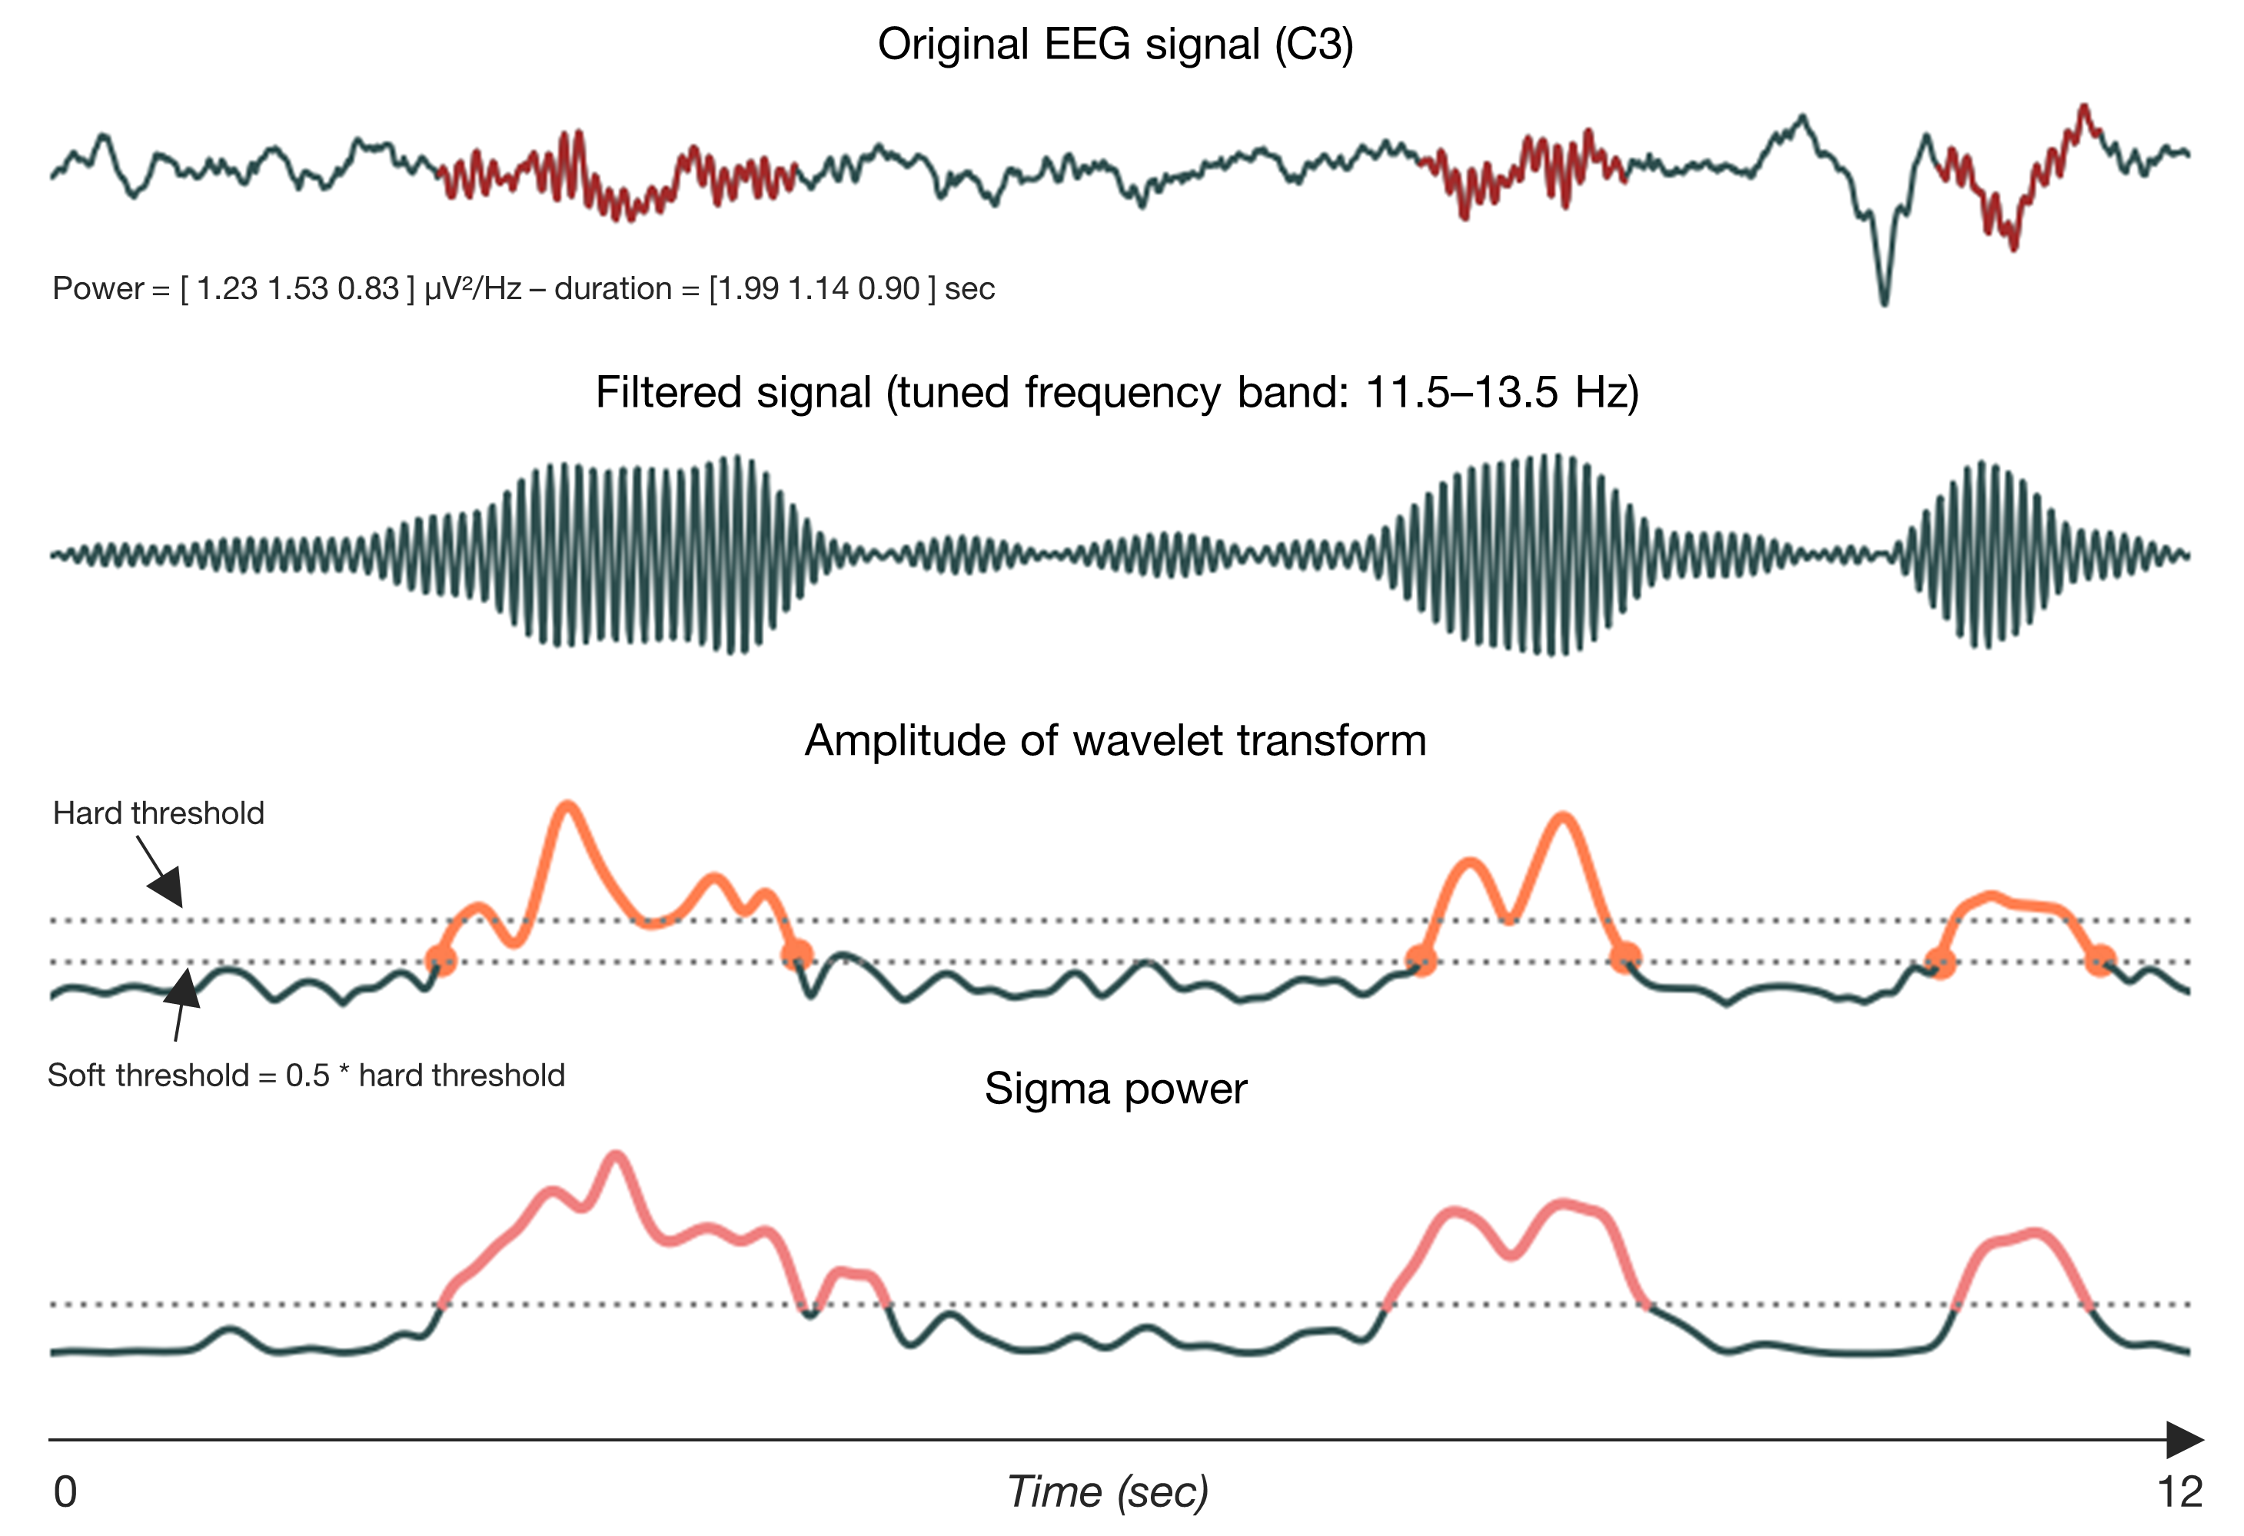
\includegraphics[width=\textwidth]{Fig/Discussion/spindles.png}
	\caption[Improved spindles detection algorithm]{\textbf{Improved spindles detection algorithm.} Compared to the initial algorithm (presented in chapter \ref{res:software}), the new spindles detection has several improvements. First, we implemented a data-driven tuning of the spindle frequency band by finding the peak spectral power within the sigma range. This step, described by \citet{berthomier_automatic_2007}, allows to accommodate for inter-individual variability of EEG signals, and is particularly useful when analyzing patients who tend to exhibit higher variability. Second, we now use both a hard and a soft threshold on the amplitude of the wavelet transform to determine more precisely the beginning and the end of each spindle. Finally, to allow users to better understand how the detection algorithm works, we implemented a function to plot the current figure for each desired time window.}
	\label{fig:disc:methods:future:spindles}
\end{figure}

Furthermore, perhaps one of the most challenging issue in sleep research is the scoring of sleep stages. Currently, the gold standard remains visual scoring by an expert, which is time-consuming and subject to high inter-rater variability. There is therefore a crucial need for reliable and time-efficient algorithms capable of detecting sleep stages in healthy and patients alike. With this in mind, we are currently working on two distinct automatic sleep scoring methods, based respectively on spectral feature extraction / microstructural detection (Fig \ref{fig:disc:methods:future:autoscore}), and on machine-learning algorithms. Preliminary results based on the former method show a 81\% agreement with a manually scored standard reference, a figure comprised within the range of human inter-scorer agreements (generally between 80 and 90\%, see \citealp{silber_visual_2007}). A similar agreement was obtained using the second, machine-learning based automatic sleep scoring method. Future developments will be needed to get the most out of these two methods and ultimately provide a state-of-the-art algorithm.

\begin{figure}[htb]
	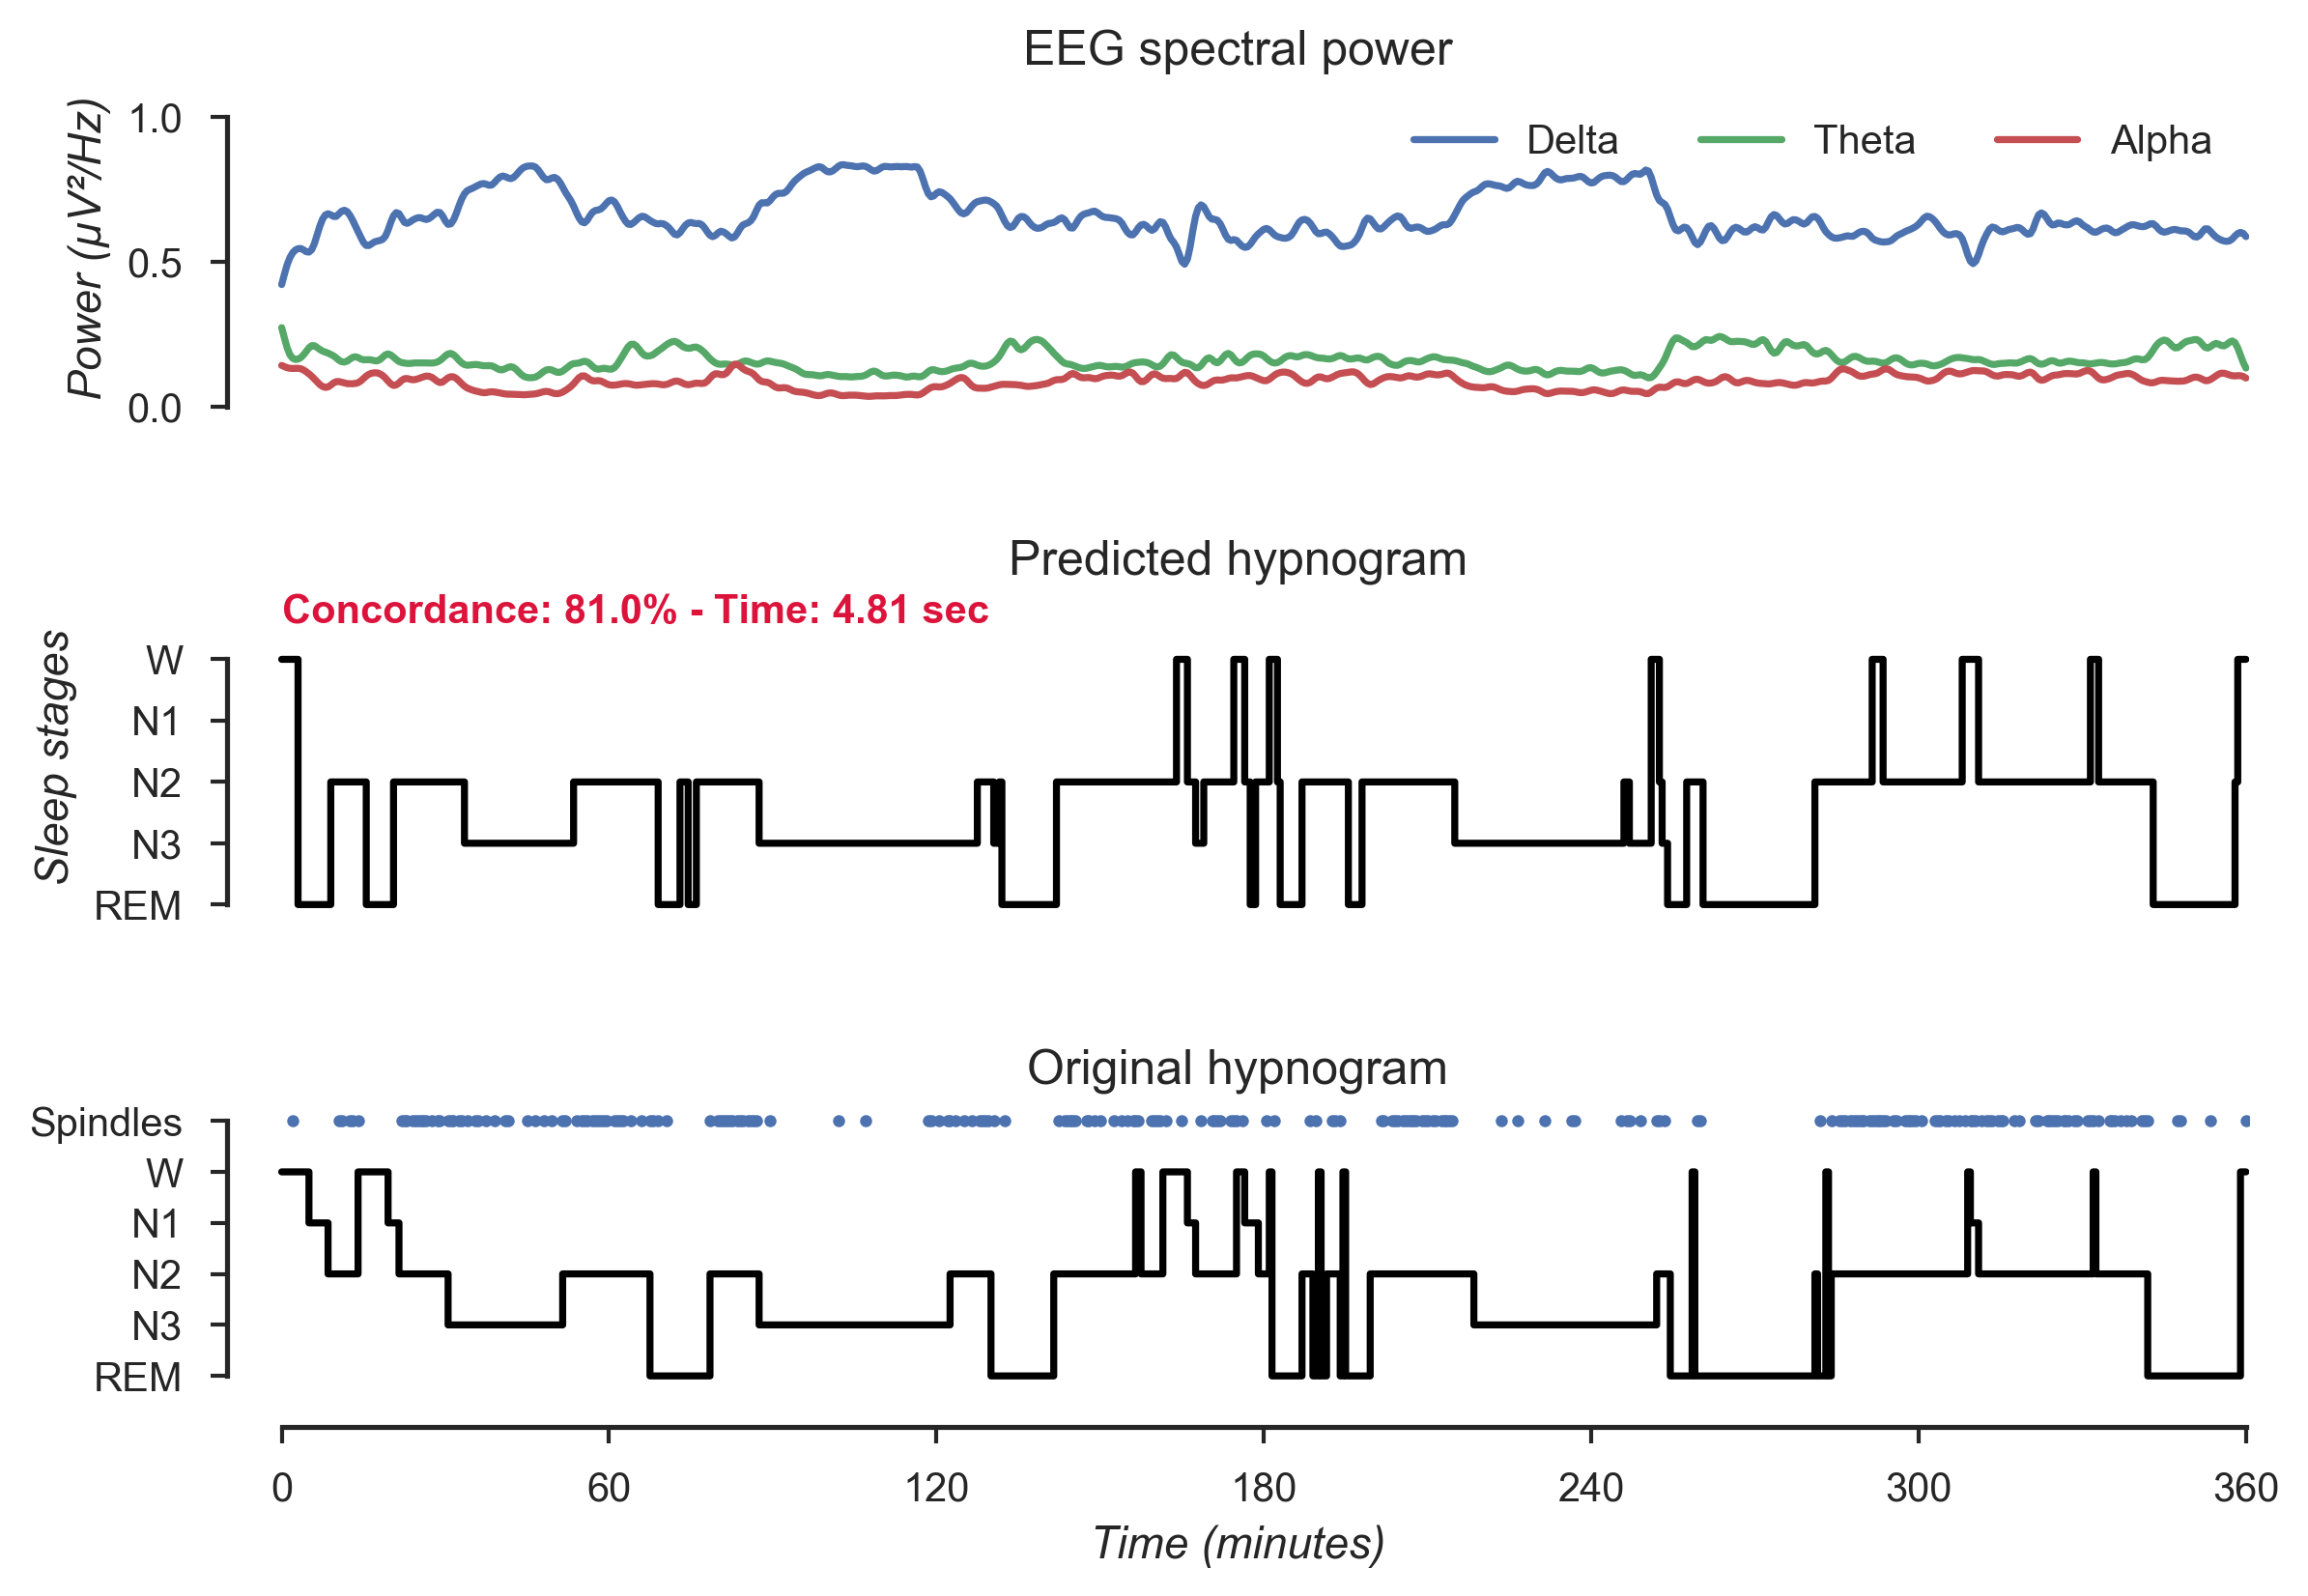
\includegraphics[width=\textwidth]{Fig/Discussion/autoscore.png}
	\caption[Preliminary results of the automatic sleep scoring algorithm]{\textbf{Preliminary results of the automatic sleep scoring algorithm.} The algorithm is based on a combination of spectral features extraction (Top) and automatic detection of microstructural features (e.g. spindles, blue dots). Preliminary tests on a single EEG channel (C3) of one healthy individual yielded 81\% agreement between the predicted and the manually scored full night hypnogram (with a running time inferior to 5 seconds).}
	\label{fig:disc:methods:future:autoscore}
\end{figure}

% Because this software represents one of the very few open-source, free and exhaustive solution for sleep reading, scoring and analysis, it will probably reach in the near future a large public of sleep researchers, students and engineers, and hopefully lead to many great collaborations. These collaborations will be facilitated by the wide range of natively supported file formats, which allows sleep laboratories across the world to visualize and analyze their sleep data using a single, common software. In conclusion, we believe that the development of SLEEP represents a major step forward in sleep research, and more broadly in the emerging philosophy of open science.

Finally, it is also important to consider that SLEEP is part of a larger package, in which the author of the present thesis is a main contributor, entitled \href{http://visbrain.org/}{Visbrain}. Visbrain is a high-performance open source visualization suite dedicated to neuroscientific data at large. It currently includes 6 visualization modules, among which the three most prominent are SLEEP, BRAIN and SIGNAL. The BRAIN module is dedicated to EEG, magneto-encephalographic (MEG) and intra-cranial recordings, and allows notably the visualization of connectivity, sources and regions of interests on a 3D brain template. The SIGNAL module is dedicated to the visualization of uni- or multi-dimensional time-series arrays, and offers as such a convenient way to inspect datasets, locate artifacts and quickly analyze time-frequency properties of time-series. We are currently working on connecting the SIGNAL and the SLEEP module, notably through the visualization of automatically detected microstructural sleep events (e.g. spindles) inside the SIGNAL module. This will provide the users an interface to identify, at a glance, the false-positive events, and allow them to further investigate the time-frequency properties of each or all events.

%%%%%%%%%%%%%%%%%%%%%%%%%%%%%%%%%%%%%%%%%%%%%%%%%%%%%%%%%%%%%%%%%%%%%%%%%%%%%%%
\cleardoublepage
\chapter{General conclusion}
\label{disc:conclusion}

Throughout this work, we have addressed several unresolved issue related to the nature, the physiological correlates, and the function of dreaming. A large part of the present thesis was devoted to comparing cognitive and neurophysiological variables in high and low dream recallers, in an effort to understand \q{what cause sleepers sometimes dream, and sometimes do not} (Aristotle, On Sleep and Sleeplessness, 350 B.C., see section \ref{sec:dream-recall}). Our results revealed that the ability to recall dream is positively associated with (1) a longer duration of intra-sleep awakenings during sleep, (2) the strength of functional connectivity in specific areas of the brain during sleep, wakefulness, and notably the period following awakening and (3) creative-thinking abilities. Based on all these findings, we proposed a new model of the dream recall process integrating the contribution of all these factors as well as their interactions. A second aspect of our work was to better understand the relationship between waking life and dream content, through an exhaustive analysis of the characteristics of waking-life memories incorporated into dreams. Our findings, in addition with providing insights on the \emph{stuff that dreams are made on}, remarkably suggest the existence of a down-regulation of emotional waking memories during dreaming. Finally, we have been committed to developing a free and comprehensive software dedicated to sleep analysis, which will hopefully represent an important step forward in sleep research by providing students, researchers and engineers a common and portable platform for their analyses. Therefore, and although much works remain to be done, the present thesis opened up a new chapter in the understanding of this fascinating phenomenon that is dreaming. The theoretical and methodological contributions of the present work could serve as a basis for future research, in the hope that someday, we will be able to fully apprehend dreaming, in all its richness and diversity.


\cleardoublepage

% --------------------------
% Back matter
% --------------------------
% \part{REFERENCES} \cleardoublepage
% {
% \setstretch{1.1}
% \renewcommand{\bibfont}{\normalfont\small}
% \setlength{\biblabelsep}{0.2pt}
% \setlength{\bibitemsep}{0.5\baselineskip plus 0.5\baselineskip}
% \printbibliography[nottype=online, heading=none]
% }
%
% \cleardoublepage
% \pagestyle{empty}
\hfill
\vfill
\section*{Colophon}

This thesis was typeset with \LaTeXe.
It uses the \textit{Clean Thesis} style developed by Ricardo Langner (\url{http://cleanthesis.der-ric.de/}).


% **************************************************
% End of Document CONTENT
% **************************************************
\cleardoublepage
\end{document}
